% ============================================================
%  يُترجَم بـ XeLaTeX  (في Overleaf: Menu → Compiler → XeLaTeX)
%  الخط: Amiri (متوفر في Overleaf، أو حمّله من github.com/aliftype/amiri)
% ============================================================
\documentclass[12pt,a4paper]{article}
\usepackage[a4paper,margin=1.7cm,top=2.3cm,bottom=2.9cm,headheight=15pt,footskip=1.5cm]{geometry}
\usepackage{amsmath,amssymb}
\usepackage{icomma}
\usepackage[english,bidi=default,layout=lists]{babel}
\babelprovide[import,main]{arabic}
\babelfont{rm}[Scale=1.08]{Amiri}
\babelfont{sf}[Scale=1.08]{Amiri}
\usepackage[most]{tcolorbox}
\usepackage{tikz}
\usetikzlibrary{arrows.meta,calc,shadings}
\usepackage{array}
\usepackage{colortbl}
\usepackage{fancyhdr}
\usepackage{titlesec}
\usepackage{enumitem}
\usepackage{collcell}
\usepackage{needspace}
\usepackage{etoolbox}
\newcolumntype{C}{>{\collectcell\ar}c<{\endcollectcell}}
\pretocmd{\section}{\Needspace{15\baselineskip}}{}{}
\pretocmd{\subsection}{\Needspace{11\baselineskip}}{}{}

\definecolor{cDef}{HTML}{1F4E9C}
\definecolor{cThm}{HTML}{B3261E}
\definecolor{cRem}{HTML}{2E7D32}
\definecolor{cEx}{HTML}{C76B00}
\definecolor{cMeth}{HTML}{6A1B9A}
\definecolor{cSol}{HTML}{00695C}
\definecolor{cSec}{HTML}{1F3A68}

\titleformat{\section}{\Large\bfseries\color{cSec}}{\thesection.}{0.6em}{}[{\color{cSec!60}\titlerule[1pt]}]
\titleformat{\subsection}{\large\bfseries\color{cThm!85!black}}{\thesubsection.}{0.5em}{}
\titlespacing*{\section}{0pt}{14pt}{8pt}
\titlespacing*{\subsection}{0pt}{10pt}{5pt}
\setlength{\parindent}{0pt}
\setlength{\parskip}{4pt}
\setlist{itemsep=2pt,topsep=3pt}

\newtcolorbox{arbox}[3][]{enhanced,
  colback=#2!5,colframe=#2!80!black,arc=2mm,boxrule=0.8pt,
  left=6pt,right=6pt,top=8pt,bottom=5pt,
  fonttitle=\bfseries,coltitle=white,
  title={\foreignlanguage{arabic}{#3}},
  attach boxed title to top right={xshift=-5mm,yshift=-3mm},
  boxed title style={colback=#2!80!black,arc=1.5mm,boxrule=0pt},
  before upper={\selectlanguage{arabic}},
  before skip=8pt,after skip=8pt,breakable,#1}
\newenvironment{BOX}[2]{\begin{otherlanguage}{english}\begin{arbox}{#1}{#2}}{\end{arbox}\end{otherlanguage}}
\newenvironment{tarif}[1][تعريف]{\begin{BOX}{cDef}{#1}}{\end{BOX}}
\newenvironment{khassia}[1][خاصية]{\begin{BOX}{cThm}{#1}}{\end{BOX}}
\newenvironment{molahada}[1][ملاحظة]{\begin{BOX}{cRem}{#1}}{\end{BOX}}
\newenvironment{mithal}[1][مثال]{\begin{BOX}{cEx}{#1}}{\end{BOX}}
\newenvironment{tariqa}[1][طريقة]{\begin{BOX}{cMeth}{#1}}{\end{BOX}}

\newcounter{exo}
\newenvironment{tamrin}[1]{\stepcounter{exo}\begin{BOX}{cSec}{التمرين \theexo: #1}}{\end{BOX}}
\newenvironment{hal}{\Needspace{12\baselineskip}\begin{otherlanguage}{english}\begin{arbox}[breakable]{cSol}{حل التمرين \theexo}}{\end{arbox}\end{otherlanguage}}

\newenvironment{LTR}{\begin{otherlanguage}{english}}{\end{otherlanguage}}
\newcommand{\ar}[1]{\foreignlanguage{arabic}{#1}}

\renewcommand{\dots}{\mathinner{\ldotp\ldotp\ldotp}}
\renewcommand{\ldots}{\mathinner{\ldotp\ldotp\ldotp}}
\renewcommand{\cdots}{\mathinner{\cdotp\cdotp\cdotp}}
\newcommand{\N}{\mathbb{N}}
\newcommand{\Z}{\mathbb{Z}}
\newcommand{\D}{\mathbb{D}}
\newcommand{\Q}{\mathbb{Q}}
\newcommand{\R}{\mathbb{R}}
\newcommand{\pgcd}{\operatorname{PGCD}}
\newcommand{\ppcm}{\operatorname{PPCM}}

% \NLseg{a}{b}{[}{]} ; \NLright{a}{[} ; \NLleft{b}{]}  (interval on a number line)
\newcommand{\NLseg}[4]{\begin{LTR}\begin{tikzpicture}[baseline=-0.6ex]
 \draw[-{Stealth[length=2mm]},gray!70](0,0)--(3.4,0);
 \draw[line width=2pt,cThm!80!black](0.7,0)--(2.7,0);
 \node[cThm!80!black,font=\LARGE] at (0.7,0){$#3$};
 \node[cThm!80!black,font=\LARGE] at (2.7,0){$#4$};
 \node[below=3pt,font=\footnotesize] at (0.7,0){$#1$};
 \node[below=3pt,font=\footnotesize] at (2.7,0){$#2$};
\end{tikzpicture}\end{LTR}}
\newcommand{\NLright}[2]{\begin{LTR}\begin{tikzpicture}[baseline=-0.6ex]
 \draw[-{Stealth[length=2mm]},gray!70](0,0)--(3.4,0);
 \draw[line width=2pt,cThm!80!black](1.3,0)--(3.3,0);
 \node[cThm!80!black,font=\LARGE] at (1.3,0){$#2$};
 \node[below=3pt,font=\footnotesize] at (1.3,0){$#1$};
\end{tikzpicture}\end{LTR}}
\newcommand{\NLleft}[2]{\begin{LTR}\begin{tikzpicture}[baseline=-0.6ex]
 \draw[-{Stealth[length=2mm]},gray!70](0,0)--(3.4,0);
 \draw[line width=2pt,cThm!80!black](0.05,0)--(2.1,0);
 \node[cThm!80!black,font=\LARGE] at (2.1,0){$#2$};
 \node[below=3pt,font=\footnotesize] at (2.1,0){$#1$};
\end{tikzpicture}\end{LTR}}

% ---------- social-media icons (pure TikZ) ----------
\definecolor{cFB}{HTML}{1877F2}
\definecolor{cTG}{HTML}{229ED9}
\definecolor{cIG1}{HTML}{FEDA75}
\definecolor{cIG2}{HTML}{D62976}
\definecolor{cIG3}{HTML}{4F5BD5}
\newcommand{\fbicon}{\begin{LTR}\begin{tikzpicture}[baseline=-0.75ex,x=1em,y=1em]
 \fill[cFB] (0,0) circle (0.55);
 \node[white,inner sep=0,font=\usefont{TU}{lmss}{bx}{n}\small] at (0.04,-0.02) {f};
\end{tikzpicture}\end{LTR}}
\newcommand{\igicon}{\begin{LTR}
\begin{tikzpicture}[baseline=-0.75ex,x=1em,y=1em]
 \shade[lower left=cIG1,lower right=cIG2,upper left=cIG2,upper right=cIG3,rounded corners=0.28em] (-0.55,-0.55) rectangle (0.55,0.55);
 \draw[white,line width=0.09em,rounded corners=0.18em] (-0.36,-0.36) rectangle (0.36,0.36);
 \draw[white,line width=0.09em] (0,0) circle (0.17);
 \fill[white] (0.22,0.22) circle (0.05);
\end{tikzpicture}\end{LTR}}
\newcommand{\tgicon}{\begin{LTR}
\begin{tikzpicture}[baseline=-0.75ex,x=1em,y=1em]
 \fill[cTG] (0,0) circle (0.55);
 \fill[white] (-0.33,0.0) -- (0.32,0.27) -- (0.2,-0.3) -- (0.0,-0.15) -- (-0.08,-0.28) -- (-0.08,-0.08) -- cycle;
 \fill[cTG!70!black] (-0.08,-0.08) -- (0.25,0.2) -- (0.0,-0.15) -- (-0.08,-0.28) -- cycle;
\end{tikzpicture}\end{LTR}}
% page number: black box, white two-digit number, at the right of the social row
\newcommand{\PageBox}{\begin{LTR}\tikz[baseline=(p.base)]\node[fill=black,text=white,inner sep=2.5pt,minimum width=1.6em,minimum height=1.3em,font=\usefont{TU}{lmss}{bx}{n}\small](p){\ifnum\value{page}<10 0\fi\arabic{page}};\end{LTR}}
% visual left-to-right order: Telegram | Instagram | Facebook | page box
\newcommand{\SocialRow}{\begin{otherlanguage}{english}%
 \ar{\textbf{الأستاذ سوايسية هشام للرياضيات}}\ \tgicon\hfill
 \textbf{prof\_hicham\_math}\ \igicon\hfill
 \ar{\textbf{الأستاذ سوايسية هشام للرياضيات}}\ \fbicon\hspace{2.2em}\PageBox\end{otherlanguage}}

\pagestyle{fancy}
\fancyhf{}
\renewcommand{\headrulewidth}{0.6pt}
\renewcommand{\footrulewidth}{0.4pt}
% \SetHeader{right head: document title}{left head: level -- stream}
\newcommand{\SetHeader}[2]{%
 \fancyhead[C]{\parbox{\textwidth}{\ar{#1\hfill #2}}}%
 \fancyfoot[C]{\parbox{\textwidth}{\small\SocialRow}}}
\usepackage{tkz-tab}
\usepackage{multicol}
% variation / sign table (LTR)
\newenvironment{TAB}{\par\begin{center}\begin{LTR}\begin{tikzpicture}[scale=0.95,every node/.style={font=\small}]}{\end{tikzpicture}\end{LTR}\end{center}}
% grid + axes, clipped: \begin{GR}{xmin}{xmax}{ymin}{ymax}{unit cm}
\newenvironment{GR}[5]{\par\begin{center}\begin{LTR}\begin{tikzpicture}[x=#5cm,y=#5cm,font=\footnotesize]
 \draw[gray!25,very thin] (#1,#3) grid (#2,#4);
 \draw[-{Stealth[length=2mm]}] (#1,0)--(#2+0.3,0) node[below left]{$x$};
 \draw[-{Stealth[length=2mm]}] (0,#3)--(0,#4+0.3) node[below left]{$y$};
 \node[below left] at (0,0){$O$};
 \begin{scope}\clip (#1,#3) rectangle (#2,#4);}
{\end{scope}\end{tikzpicture}\end{LTR}\end{center}}
\newcommand{\Ticks}[2]{\foreach \t in {#1} \node[below,font=\scriptsize] at (\t,0){$\t$}; \foreach \t in {#2} \node[left,font=\scriptsize] at (0,\t){$\t$};}
\newcommand{\bx}[1]{\ensuremath{\colorbox{cDef!12}{$\displaystyle #1$}}}
\newcommand{\TwoCol}[4]{\par\begin{LTR}\noindent\begin{minipage}[t]{#1\textwidth}\selectlanguage{arabic}#2\end{minipage}\hfill\begin{minipage}[t]{#3\textwidth}\selectlanguage{arabic}#4\end{minipage}\end{LTR}\par}
\newcommand{\RL}[4]{\TwoCol{#3}{#4}{#1}{#2}}  % \RL{w1}{right content}{w2}{left content}
\newcommand{\ok}{$\textcolor{cRem}{\checkmark}$}
\newcommand{\limn}{\displaystyle\lim_{n\to+\infty}}
% sub-questions, each on its own line
\newenvironment{sq}{\begin{itemize}[leftmargin=2.4em,itemsep=3pt]}{\end{itemize}}
\newcommand{\qa}{\item[(أ)]}\newcommand{\qb}{\item[(ب)]}\newcommand{\qc}{\item[(جـ)]}\newcommand{\qd}{\item[(د)]}\newcommand{\qe}{\item[(هـ)]}
\newcommand{\pa}{\par\smallskip\textbf{(أ)} }\newcommand{\pb}{\par\smallskip\textbf{(ب)} }\newcommand{\pc}{\par\smallskip\textbf{(جـ)} }\newcommand{\pd}{\par\smallskip\textbf{(د)} }\newcommand{\pe}{\par\smallskip\textbf{(هـ)} }
\newcommand{\QQ}[1]{\par\smallskip\textbf{#1.} }
\newenvironment{tmr}{\stepcounter{exo}\begin{BOX}{cSec}{تمرين محلول \theexo}}{\end{BOX}}
\newcommand{\ABC}[3]{\\[2pt]\begin{tabular}{p{0.28\textwidth}p{0.28\textwidth}p{0.28\textwidth}}(جـ) \ #3 & (ب) \ #2 & (أ) \ #1\end{tabular}}
\pretocmd{\section}{\Needspace{24\baselineskip}}{}{}
\newtcbox{\bxtbox}{on line,colback=cDef!12,colframe=cDef!12,boxrule=0pt,arc=1pt,boxsep=0pt,left=2pt,right=2pt,top=1pt,bottom=1pt}
\newcommand{\bxt}[1]{\foreignlanguage{english}{\bxtbox{\ar{#1}}}}
\SetHeader{\small\bfseries\color{cSec}تمارين البكالوريا: الأعداد المركبة والتحويلات النقطية}{\small\color{cSec}السنة الثالثة ثانوي -- الشعب العلمية}
\begin{document}
\begin{LTR}
\begin{tcolorbox}[enhanced,colback=cSec,colframe=cSec,arc=3mm,halign=center,boxrule=0pt,top=12pt,bottom=12pt,before upper={\selectlanguage{arabic}}]
{\color{white}\fontsize{24}{30}\selectfont\bfseries تمارين البكالوريا في الأعداد المركبة والتحويلات النقطية}\\[8pt]
{\color{white}\large مع الحلول المفصلة -- حتى دورة 2026}\\[5pt]
{\color{white}\large علوم تجريبية -- تقني رياضي -- رياضيات}
\end{tcolorbox}
\end{LTR}
\section{تمارين البكالوريا -- شعبة علوم تجريبية}
% ===================== التمرين 1 =====================
\Needspace{12\baselineskip}
\begin{tamrin}{بكالوريا 2026 -- الموضوع الأول -- علوم تجريبية}
\textbf{I)} حل في المجموعة $\mathbb{C}$ المعادلة ذات المجهول $z$ التالية: $(iz+4)(z^2-4z+16)=0$.

\textbf{II)} المستوي المركب منسوب إلى المعلم المتعامد والمتجانس $(O;\vec u,\vec v)$، و$A$، $B$، $C$ و$D$ نقط من المستوي لاحقاتها على الترتيب $z_A=4$، $z_B=iz_A$، $z_C=2-2i\sqrt3$ و$z_D=-iz_C$.
\QQ{1}
\begin{sq}
\qa أكتب كلا من $z_B$، $z_C$ و$z_D$ على الشكل المثلثي.
\qb علم النقط $A$، $B$، $C$ و$D$ ثم تحقق أنها تنتمي إلى نفس الدائرة التي يطلب تعيين مركزها ونصف قطرها.
\end{sq}
\QQ{2}
\begin{sq}
\qa أبرز أن: $z_D-z_B=\sqrt3\,(z_C-z_A)$ ثم استنتج أن المستقيمين $(BD)$ و$(AC)$ متوازيان.
\qb بين أن: $|z_B-z_A|=|z_D-z_C|$.
\qc استنتج طبيعة الرباعي $ABDC$ ثم عين لاحقة النقطة $G$ مركز ثقله.
\end{sq}
\QQ{3} تحقق أن: $z_D-z_A=i\,(z_B-z_C)$ ثم عين الأعداد الطبيعية $n$ حتى يكون $\left(\dfrac{z_D-z_A}{z_B-z_C}\right)^{n}$ عددا حقيقيا.
\end{tamrin}

\begin{hal}
\textbf{I) حل المعادلة.} الجداء معدوم يعني أحد عامليه معدوم:
\begin{itemize}
\item $iz+4=0$ يعني $iz=-4$ أي $z=\dfrac{-4}{i}=\dfrac{-4\times(-i)}{i\times(-i)}=4i$.
\item $z^2-4z+16=0$: المميز $\Delta=(-4)^2-4\times1\times16=16-64=-48=\left(4i\sqrt3\right)^2$، و$\Delta<0$ إذن للمعادلة حلان مركبان مترافقان:
$z_1=\dfrac{4-4i\sqrt3}{2}=2-2i\sqrt3$ و$z_2=\overline{z_1}=2+2i\sqrt3$.
\end{itemize}
إذن \bx{S=\left\{4i\,;\,2-2i\sqrt3\,;\,2+2i\sqrt3\right\}}.

\textbf{II)} لدينا $z_B=iz_A=4i$ و$z_D=-i\left(2-2i\sqrt3\right)=-2i+2i^2\sqrt3=-2\sqrt3-2i$.

\QQ{1}
\pa $z_B=4i$: طويلته $4$ وعمدة له $\dfrac{\pi}{2}$ إذن \bx{z_B=4\left(\cos\tfrac{\pi}{2}+i\sin\tfrac{\pi}{2}\right)}.

$|z_C|=\sqrt{2^2+\left(2\sqrt3\right)^2}=\sqrt{16}=4$، و$\cos\theta=\dfrac{2}{4}=\dfrac12$، $\sin\theta=\dfrac{-2\sqrt3}{4}=-\dfrac{\sqrt3}{2}$ إذن $\theta=-\dfrac{\pi}{3}$:
\bx{z_C=4\left(\cos\left(-\tfrac{\pi}{3}\right)+i\sin\left(-\tfrac{\pi}{3}\right)\right)}.

$z_D=-iz_C$ و$-i=\cos\left(-\tfrac{\pi}{2}\right)+i\sin\left(-\tfrac{\pi}{2}\right)$، إذن $|z_D|=1\times4=4$ و$\arg z_D=-\dfrac{\pi}{2}-\dfrac{\pi}{3}=-\dfrac{5\pi}{6}$:
\bx{z_D=4\left(\cos\left(-\tfrac{5\pi}{6}\right)+i\sin\left(-\tfrac{5\pi}{6}\right)\right)}.

\pb لدينا $|z_A|=|z_B|=|z_C|=|z_D|=4$ أي $OA=OB=OC=OD=4$، إذن النقط الأربع تنتمي إلى
\bxt{الدائرة التي مركزها $O$ ونصف قطرها $4$}.

\begin{center}\begin{LTR}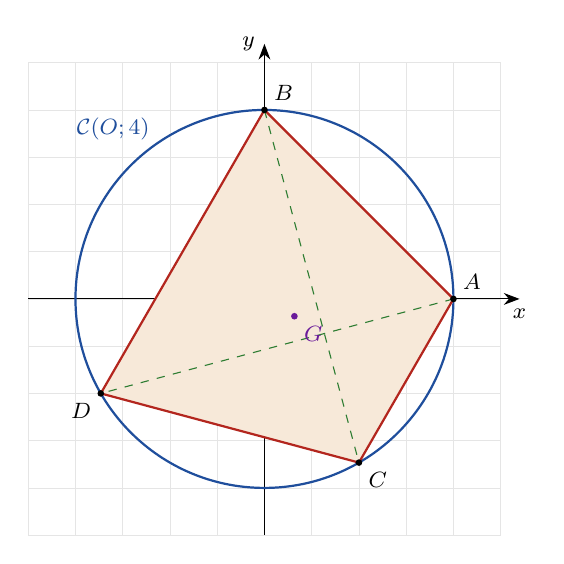
\begin{tikzpicture}[scale=0.6,font=\footnotesize]
\draw[gray!20,very thin](-5,-5) grid (5,5);
\draw[-{Stealth[length=2mm]}](-5,0)--(5.4,0) node[below]{$x$};
\draw[-{Stealth[length=2mm]}](0,-5)--(0,5.4) node[left]{$y$};
\draw[-{Stealth[length=2mm]},thick](0,0)--(1,0) node[below]{$\vec u$};
\draw[-{Stealth[length=2mm]},thick](0,0)--(0,1) node[left]{$\vec v$};
\node[below left] at (0,0){$O$};
\draw[cDef,thick](0,0) circle (4);
\fill[cEx!15](4,0)--(0,4)--(-3.464,-2)--(2,-3.464)--cycle;
\draw[cThm,thick](4,0)--(0,4)--(-3.464,-2)--(2,-3.464)--cycle;
\draw[cRem,dashed](4,0)--(-3.464,-2) (0,4)--(2,-3.464);
\fill (4,0) circle (2pt) node[above right]{$A$};
\fill (0,4) circle (2pt) node[above right]{$B$};
\fill (2,-3.464) circle (2pt) node[below right]{$C$};
\fill (-3.464,-2) circle (2pt) node[below left]{$D$};
\fill[cMeth] (0.634,-0.366) circle (2pt) node[below right]{$G$};
\node[cDef] at (-3.2,3.6){$\mathcal{C}(O;4)$};
\end{tikzpicture}\end{LTR}\end{center}

\QQ{2}
\pa $z_D-z_B=-2\sqrt3-2i-4i=-2\sqrt3-6i$.\\
$\sqrt3\,(z_C-z_A)=\sqrt3\left(2-2i\sqrt3-4\right)=\sqrt3\left(-2-2i\sqrt3\right)=-2\sqrt3-6i$.\\
إذن \bx{z_D-z_B=\sqrt3\,(z_C-z_A)}، ومعناه $\overrightarrow{BD}=\sqrt3\,\overrightarrow{AC}$: الشعاعان مرتبطان خطيا، إذن \bx{(BD)\parallel(AC)}.

\pb $|z_B-z_A|=|-4+4i|=\sqrt{16+16}=4\sqrt2$.\\
$z_D-z_C=-2\sqrt3-2i-2+2i\sqrt3=\left(-2-2\sqrt3\right)+i\left(2\sqrt3-2\right)$، ومنه
$|z_D-z_C|^2=\left(2+2\sqrt3\right)^2+\left(2\sqrt3-2\right)^2=(16+8\sqrt3)+(16-8\sqrt3)=32$، أي $|z_D-z_C|=4\sqrt2$.
إذن \bx{|z_B-z_A|=|z_D-z_C|=4\sqrt2} أي $AB=CD$.

\pc في الرباعي $ABDC$ (الأضلاع $[AB]$، $[BD]$، $[DC]$، $[CA]$): الضلعان $[BD]$ و$[AC]$ متوازيان وغير متقايسين ($BD=\sqrt3\,AC$)، إذن هو شبه منحرف قاعدتاه $[BD]$ و$[AC]$، وساقاه $[AB]$ و$[DC]$ متقايستان. إذن
\bxt{$ABDC$ شبه منحرف متساوي الساقين} (وهو محاط بالدائرة السابقة).

$G$ مركز ثقل الرباعي هو مرجح النقط الأربع المرفقة بنفس المعامل:
\[z_G=\frac{z_A+z_B+z_C+z_D}{4}=\frac{4+4i+2-2i\sqrt3-2\sqrt3-2i}{4}=\frac{\left(6-2\sqrt3\right)+i\left(2-2\sqrt3\right)}{4}\]
\bx{z_G=\frac{3-\sqrt3}{2}+i\,\frac{1-\sqrt3}{2}}.

\QQ{3} $z_D-z_A=-2\sqrt3-2i-4=\left(-4-2\sqrt3\right)-2i$.\\
$z_B-z_C=4i-2+2i\sqrt3=-2+i\left(4+2\sqrt3\right)$، ومنه $i(z_B-z_C)=-2i+i^2\left(4+2\sqrt3\right)=\left(-4-2\sqrt3\right)-2i$.\\
إذن \bx{z_D-z_A=i\,(z_B-z_C)} ومنه $\dfrac{z_D-z_A}{z_B-z_C}=i=e^{i\frac{\pi}{2}}$.

$\left(\dfrac{z_D-z_A}{z_B-z_C}\right)^n=i^n=e^{i\frac{n\pi}{2}}$ يكون حقيقيا إذا وفقط إذا كان $\dfrac{n\pi}{2}=k\pi$ ($k\in\mathbb{Z}$) أي $n=2k$.
إذن \bxt{$n$ عدد طبيعي زوجي: $n=2k$ مع $k\in\mathbb{N}$}.

\textbf{تفسير:} $AD=BC$ و$(AD)\perp(BC)$: قطرا شبه المنحرف متقايسان ومتعامدان.
\end{hal}

% ===================== التمرين 2 =====================
\Needspace{12\baselineskip}
\begin{tamrin}{بكالوريا 2026 -- الموضوع الثاني -- علوم تجريبية}
\QQ{1} نعتبر في المجموعة $\mathbb{C}$ المعادلة ذات المجهول $z$ الآتية: $z^2+\alpha z+4=0 \ \ldots\ (E)$ حيث $\alpha$ عدد حقيقي.
\begin{sq}
\qa أحسب $\left(-1+i\sqrt3\right)^2$ ثم استنتج الجذرين التربيعيين للعدد $-2-2i\sqrt3$.
\qb عين $\alpha$ حتى يكون العدد المركب $-1+i\sqrt3$ حلا للمعادلة $(E)$ ثم استنتج حلها الآخر.
\end{sq}
\QQ{2} نعتبر الأعداد المركبة $z_1$، $z_2$ و$z_3$ حيث: $z_1=-1+i\sqrt3$، $z_2=-1-i\sqrt3$ و$z_3=\sqrt2\,(1-i)$.
\begin{sq}
\qa أكتب كلا من $z_1$، $z_2$ و$z_3$ على الشكل المثلثي.
\qb استنتج الشكل المثلثي للعدد المركب $L$ حيث: $L=\dfrac{z_1\times z_3}{z_2}$.
\qc أكتب $L$ على الشكل الجبري ثم استنتج القيمة المضبوطة لكل من $\cos\dfrac{13\pi}{12}$ و$\sin\dfrac{13\pi}{12}$.
\end{sq}
\end{tamrin}

\begin{hal}
\QQ{1}
\pa $\left(-1+i\sqrt3\right)^2=1-2i\sqrt3+\left(i\sqrt3\right)^2=1-2i\sqrt3-3$ إذن \bx{\left(-1+i\sqrt3\right)^2=-2-2i\sqrt3}.

إذن الجذران التربيعيان للعدد $-2-2i\sqrt3$ هما \bx{-1+i\sqrt3} و\bx{1-i\sqrt3}.

\pb $-1+i\sqrt3$ حل للمعادلة $(E)$ يعني $\left(-1+i\sqrt3\right)^2+\alpha\left(-1+i\sqrt3\right)+4=0$، أي
\[-2-2i\sqrt3-\alpha+i\alpha\sqrt3+4=0\iff(2-\alpha)+i\sqrt3\,(\alpha-2)=0 .\]
عدد مركب معدوم يعني جزؤه الحقيقي وجزؤه التخيلي معدومان: $2-\alpha=0$ و$\alpha-2=0$، إذن \bx{\alpha=2}.

تصبح $(E)$: $z^2+2z+4=0$. جداء الحلين $z'z''=\dfrac{c}{a}=4$، ومنه الحل الآخر
$z''=\dfrac{4}{-1+i\sqrt3}=\dfrac{4\left(-1-i\sqrt3\right)}{1+3}$ أي \bx{z''=-1-i\sqrt3}
(وهو مرافق الحل الأول لأن معاملات $(E)$ حقيقية).

\QQ{2}
\pa $|z_1|=\sqrt{1+3}=2$، $\cos\theta_1=-\dfrac12$ و$\sin\theta_1=\dfrac{\sqrt3}{2}$ إذن $\theta_1=\dfrac{2\pi}{3}$:
\bx{z_1=2\left(\cos\tfrac{2\pi}{3}+i\sin\tfrac{2\pi}{3}\right)}.

$z_2=\overline{z_1}$ إذن $|z_2|=2$ و$\arg z_2=-\dfrac{2\pi}{3}$:
\bx{z_2=2\left(\cos\left(-\tfrac{2\pi}{3}\right)+i\sin\left(-\tfrac{2\pi}{3}\right)\right)}.

$|z_3|=\sqrt2\times\sqrt{1+1}=2$، $\cos\theta_3=\dfrac{\sqrt2}{2}$ و$\sin\theta_3=-\dfrac{\sqrt2}{2}$ إذن $\theta_3=-\dfrac{\pi}{4}$:
\bx{z_3=2\left(\cos\left(-\tfrac{\pi}{4}\right)+i\sin\left(-\tfrac{\pi}{4}\right)\right)}.

\pb $|L|=\dfrac{|z_1|\times|z_3|}{|z_2|}=\dfrac{2\times2}{2}=2$، و
$\arg L=\arg z_1+\arg z_3-\arg z_2=\dfrac{2\pi}{3}-\dfrac{\pi}{4}+\dfrac{2\pi}{3}=\dfrac{16\pi-3\pi}{12}=\dfrac{13\pi}{12}$.
إذن \bx{L=2\left(\cos\tfrac{13\pi}{12}+i\sin\tfrac{13\pi}{12}\right)}.

\pc $z_1z_3=\sqrt2\left(-1+i\sqrt3\right)(1-i)=\sqrt2\left(-1+i+i\sqrt3+\sqrt3\right)=\sqrt2\left[\left(\sqrt3-1\right)+i\left(\sqrt3+1\right)\right]$.

نضرب في مرافق المقام $\overline{z_2}=-1+i\sqrt3$ ($|z_2|^2=4$):
\begin{align*}
L&=\frac{\sqrt2}{4}\left[\left(\sqrt3-1\right)+i\left(\sqrt3+1\right)\right]\left(-1+i\sqrt3\right)
=\frac{\sqrt2}{4}\left[\left(-2-2\sqrt3\right)+i\left(2-2\sqrt3\right)\right]
\end{align*}
\bx{L=-\frac{\sqrt2+\sqrt6}{2}+i\,\frac{\sqrt2-\sqrt6}{2}}.

بالمطابقة مع الشكل المثلثي $L=2\cos\tfrac{13\pi}{12}+2i\sin\tfrac{13\pi}{12}$:
\[\cos\frac{13\pi}{12}=-\frac{\sqrt6+\sqrt2}{4}\qquad\text{,}\qquad \sin\frac{13\pi}{12}=\frac{\sqrt2-\sqrt6}{4}.\]
أي \bx{\cos\tfrac{13\pi}{12}=-\tfrac{\sqrt6+\sqrt2}{4}} و\bx{\sin\tfrac{13\pi}{12}=\tfrac{\sqrt2-\sqrt6}{4}}.
\end{hal}

% ===================== التمرين 3 =====================
\Needspace{12\baselineskip}
\begin{tamrin}{بكالوريا 2025 -- الموضوع الأول -- علوم تجريبية}
\QQ{1} حل في مجموعة الأعداد المركبة $\mathbb{C}$ المعادلة ذات المجهول $z$ التالية: $(iz+2)\left(z^2+2\sqrt3\,z+4\right)=0$.
\QQ{2} المستوي المركب منسوب إلى المعلم المتعامد والمتجانس $(O;\vec u,\vec v)$. $A$، $B$ و$C$ نقط من المستوي لاحقاتها على الترتيب: $z_A=2i$، $z_B=-\sqrt3+i$ و$z_C=\overline{z_B}$.
\begin{sq}
\qa أكتب كلا من $z_A$، $z_B$ و$z_C$ على الشكل المثلثي.
\qb استنتج أن النقط $A$، $B$ و$C$ تنتمي إلى نفس الدائرة التي يطلب تعيين مركزها ونصف قطرها.
\qc حدد طبيعة المثلث $ABC$ ثم عين لاحقة مركز ثقله.
\end{sq}
\QQ{3} $z$ عدد مركب حيث $z=(\cos\theta+i\sin\theta)\,z_A$ و$\theta$ عدد حقيقي مع $0<\theta<\dfrac{\pi}{2}$.

عين قيمة $\theta$ بحيث يكون $\dfrac{5\pi}{6}$ عمدة للعدد $z$.
\end{tamrin}

\begin{hal}
\QQ{1}
\begin{itemize}
\item $iz+2=0$ يعني $z=\dfrac{-2}{i}=2i$.
\item $z^2+2\sqrt3\,z+4=0$: $\Delta=12-16=-4=(2i)^2$، إذن $z=\dfrac{-2\sqrt3-2i}{2}=-\sqrt3-i$ أو $z=-\sqrt3+i$.
\end{itemize}
\bx{S=\left\{2i\,;\,-\sqrt3+i\,;\,-\sqrt3-i\right\}}.

\QQ{2}
\pa $z_A=2i$: \bx{z_A=2\left(\cos\tfrac{\pi}{2}+i\sin\tfrac{\pi}{2}\right)}.

$|z_B|=\sqrt{3+1}=2$، $\cos\theta=-\dfrac{\sqrt3}{2}$، $\sin\theta=\dfrac12$ إذن $\theta=\dfrac{5\pi}{6}$:
\bx{z_B=2\left(\cos\tfrac{5\pi}{6}+i\sin\tfrac{5\pi}{6}\right)}.

$z_C=\overline{z_B}=-\sqrt3-i$: \bx{z_C=2\left(\cos\left(-\tfrac{5\pi}{6}\right)+i\sin\left(-\tfrac{5\pi}{6}\right)\right)}.

\pb $|z_A|=|z_B|=|z_C|=2$ أي $OA=OB=OC=2$، إذن $A$، $B$ و$C$ تنتمي إلى
\bxt{الدائرة التي مركزها $O$ ونصف قطرها $2$}.

\pc نحسب $\dfrac{z_A-z_B}{z_C-z_B}=\dfrac{\sqrt3+i}{-2i}=\dfrac{\left(\sqrt3+i\right)i}{2}=-\dfrac12+i\dfrac{\sqrt3}{2}=e^{i\frac{2\pi}{3}}$.

إذن $\left|\dfrac{z_A-z_B}{z_C-z_B}\right|=1$ أي $BA=BC$، و$\left(\overrightarrow{BC},\overrightarrow{BA}\right)=\dfrac{2\pi}{3}$.
(تحقق: $AB=|-\sqrt3-i|=2$، $BC=|-2i|=2$، $AC=|-\sqrt3-3i|=2\sqrt3$.)

إذن \bxt{المثلث $ABC$ متساوي الساقين رأسه $B$ وزاويته الرئيسية $\frac{2\pi}{3}$}.

مركز الثقل: $z_G=\dfrac{z_A+z_B+z_C}{3}=\dfrac{2i-\sqrt3+i-\sqrt3-i}{3}$ أي \bx{z_G=-\frac{2\sqrt3}{3}+\frac23\,i}.

\begin{center}\begin{LTR}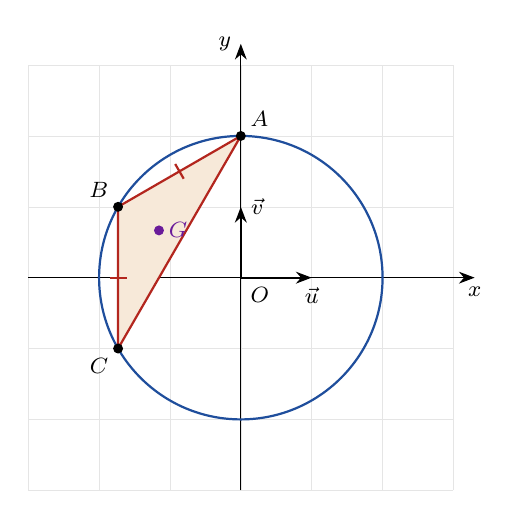
\begin{tikzpicture}[scale=0.9,font=\footnotesize]
\draw[gray!20,very thin](-3,-3) grid (3,3);
\draw[-{Stealth[length=2mm]}](-3,0)--(3.3,0) node[below]{$x$};
\draw[-{Stealth[length=2mm]}](0,-3)--(0,3.3) node[left]{$y$};
\draw[-{Stealth[length=2mm]},thick](0,0)--(1,0) node[below]{$\vec u$};
\draw[-{Stealth[length=2mm]},thick](0,0)--(0,1) node[right]{$\vec v$};
\node[below right] at (0,0){$O$};
\draw[cDef,thick](0,0) circle (2);
\fill[cEx!15](0,2)--(-1.732,1)--(-1.732,-1)--cycle;
\draw[cThm,thick](0,2)--(-1.732,1)--(-1.732,-1)--cycle;
\draw[cThm,thick]($(0,2)!0.5!(-1.732,1)$)++(-60:0.12)--++(120:0.24);
\draw[cThm,thick]($(-1.732,1)!0.5!(-1.732,-1)$)++(0:0.12)--++(180:0.24);
\fill (0,2) circle (2pt) node[above right]{$A$};
\fill (-1.732,1) circle (2pt) node[above left]{$B$};
\fill (-1.732,-1) circle (2pt) node[below left]{$C$};
\fill[cMeth] (-1.155,0.667) circle (2pt) node[right]{$G$};
\end{tikzpicture}\end{LTR}\end{center}

\QQ{3} $z=(\cos\theta+i\sin\theta)\times2\left(\cos\tfrac{\pi}{2}+i\sin\tfrac{\pi}{2}\right)=2\left(\cos\left(\theta+\tfrac{\pi}{2}\right)+i\sin\left(\theta+\tfrac{\pi}{2}\right)\right)$،
إذن $\arg z=\theta+\dfrac{\pi}{2}+2k\pi$.

$\dfrac{5\pi}{6}$ عمدة للعدد $z$ يعني $\theta+\dfrac{\pi}{2}=\dfrac{5\pi}{6}+2k\pi$ أي $\theta=\dfrac{\pi}{3}+2k\pi$، ومع $0<\theta<\dfrac{\pi}{2}$ نجد $k=0$:
\bx{\theta=\frac{\pi}{3}}.
\end{hal}

% ===================== التمرين 4 =====================
\Needspace{12\baselineskip}
\begin{tamrin}{بكالوريا 2025 -- الموضوع الثاني -- علوم تجريبية}
\QQ{1} أنشر $(1+i)^2$ ثم حل في مجموعة الأعداد المركبة $\mathbb{C}$ المعادلة ذات المجهول $z$ التالية: $z^2=8i$.
\QQ{2} المستوي المركب منسوب إلى المعلم المتعامد والمتجانس $(O;\vec u,\vec v)$. $A$، $B$ و$C$ نقط من المستوي لاحقاتها على الترتيب: $z_A=2+2i$، $z_B=-z_A$ و$z_C=\overline{z_B}$.
\begin{sq}
\qa أكتب كلا من $z_A$، $z_B$ و$z_C$ على الشكل المثلثي.
\qb استنتج أن النقط $A$، $B$ و$C$ تنتمي إلى نفس الدائرة التي يطلب تعيين مركزها ونصف قطرها.
\end{sq}
\QQ{3} تحقق أن: $z_A-z_C=i\,(z_B-z_C)$ ثم حدد طبيعة المثلث $ABC$.
\QQ{4} عين $z_D$ و$z_E$ لاحقتي النقطتين $D$ و$E$ على الترتيب حتى تكون النقطة $C$ مركز المربع $ABDE$.
\end{tamrin}

\begin{hal}
\QQ{1} $(1+i)^2=1+2i+i^2$ إذن \bx{(1+i)^2=2i}.

ومنه $8i=4\times2i=4(1+i)^2=\left(2(1+i)\right)^2=(2+2i)^2$. المعادلة $z^2=(2+2i)^2$ تكافئ $(z-2-2i)(z+2+2i)=0$:
\bx{S=\{2+2i\,;\,-2-2i\}}.

\QQ{2} $z_A=2+2i$، $z_B=-2-2i$، $z_C=\overline{z_B}=-2+2i$.

\pa $|z_A|=\sqrt{4+4}=2\sqrt2$ و$\arg z_A=\dfrac{\pi}{4}$ (لأن $\cos\theta=\sin\theta=\frac{\sqrt2}{2}$):
\bx{z_A=2\sqrt2\left(\cos\tfrac{\pi}{4}+i\sin\tfrac{\pi}{4}\right)}.

$z_B=-z_A$ إذن $|z_B|=2\sqrt2$ و$\arg z_B=\dfrac{\pi}{4}+\pi\equiv-\dfrac{3\pi}{4}$:
\bx{z_B=2\sqrt2\left(\cos\left(-\tfrac{3\pi}{4}\right)+i\sin\left(-\tfrac{3\pi}{4}\right)\right)}.

$z_C=\overline{z_B}$ إذن \bx{z_C=2\sqrt2\left(\cos\tfrac{3\pi}{4}+i\sin\tfrac{3\pi}{4}\right)}.

\pb $OA=OB=OC=2\sqrt2$، إذن النقط تنتمي إلى \bxt{الدائرة التي مركزها $O$ ونصف قطرها $2\sqrt2$}.
(بما أن $z_B=-z_A$ فإن $O$ منتصف $[AB]$: القطعة $[AB]$ قطر لهذه الدائرة.)

\QQ{3} $z_A-z_C=2+2i+2-2i=4$ و$i(z_B-z_C)=i(-2-2i+2-2i)=i(-4i)=4$، إذن \bx{z_A-z_C=i\,(z_B-z_C)}.

ومنه $\dfrac{z_A-z_C}{z_B-z_C}=i=e^{i\frac{\pi}{2}}$: إذن $CA=CB$ و$\left(\overrightarrow{CB},\overrightarrow{CA}\right)=\dfrac{\pi}{2}$،
أي \bxt{المثلث $ABC$ قائم في $C$ ومتساوي الساقين}.

\QQ{4} $C$ مركز المربع $ABDE$ يعني أن $C$ منتصف قطريه $[AD]$ و$[BE]$:
\begin{itemize}
\item $z_C=\dfrac{z_A+z_D}{2}$ ومنه $z_D=2z_C-z_A=-4+4i-2-2i$ أي \bx{z_D=-6+2i}.
\item $z_C=\dfrac{z_B+z_E}{2}$ ومنه $z_E=2z_C-z_B=-4+4i+2+2i$ أي \bx{z_E=-2+6i}.
\end{itemize}
تبرير أنه مربع: القطران متناصفان (متوازي أضلاع)، و$CA=CB$ مع $(CA)\perp(CB)$ أي القطران متقايسان ومتعامدان.

\begin{center}\begin{LTR}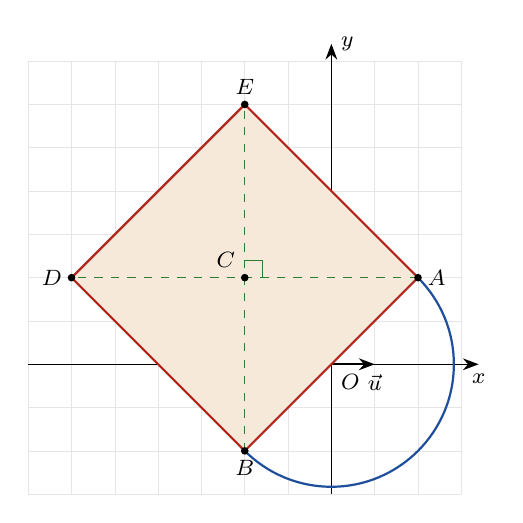
\begin{tikzpicture}[scale=0.55,font=\footnotesize]
\draw[gray!20,very thin](-7,-3) grid (3,7);
\draw[-{Stealth[length=2mm]}](-7,0)--(3.4,0) node[below]{$x$};
\draw[-{Stealth[length=2mm]}](0,-3)--(0,7.4) node[right]{$y$};
\draw[-{Stealth[length=2mm]},thick](0,0)--(1,0) node[below]{$\vec u$};
\draw[-{Stealth[length=2mm]},thick](0,0)--(0,1) node[right]{$\vec v$};
\node[below right] at (0,0){$O$};
\draw[cDef,thick](0,0) circle (2.828);
\fill[cEx!15](2,2)--(-2,-2)--(-6,2)--(-2,6)--cycle;
\draw[cThm,thick](2,2)--(-2,-2)--(-6,2)--(-2,6)--cycle;
\draw[cRem,dashed](2,2)--(-6,2) (-2,-2)--(-2,6);
\draw[cRem] (-2,2)++(0,0.4)--++(0.4,0)--++(0,-0.4);
\fill (2,2) circle (2.5pt) node[right]{$A$};
\fill (-2,-2) circle (2.5pt) node[below]{$B$};
\fill (-2,2) circle (2.5pt) node[above left]{$C$};
\fill (-6,2) circle (2.5pt) node[left]{$D$};
\fill (-2,6) circle (2.5pt) node[above]{$E$};
\end{tikzpicture}\end{LTR}\end{center}
\end{hal}

% ===================== التمرين 5 =====================
\Needspace{12\baselineskip}
\begin{tamrin}{بكالوريا 2024 -- الموضوع الأول -- علوم تجريبية}
\textbf{I)} حل في مجموعة الأعداد المركبة $\mathbb{C}$ المعادلة ذات المجهول $z$ الآتية:
\[\left(z-1+2\sqrt3\right)\left[z^2-2\left(1-\sqrt3\right)z+5-2\sqrt3\right]=0 .\]
\textbf{II)} في المستوي المنسوب إلى المعلم المتعامد والمتجانس $(O;\vec i,\vec j)$، نعتبر النقط $A$، $B$ و$C$ التي لاحقاتها على الترتيب $z_A$، $z_B$ و$z_C$ حيث: $z_A=1-\sqrt3+i$، $z_B=1-2\sqrt3$ و$z_C=\overline{z_A}$.
\QQ{1} أكتب كلا من $z_A-1$، $z_C-1$ و$z_B$ على الشكل المثلثي.
\QQ{2} جد لاحقة النقطة $D$ مرجح الجملة المثقلة $\{(A;1),(B;-1),(C;1)\}$.
\QQ{3} بين أن الرباعي $ABCD$ معين.
\end{tamrin}

\begin{hal}
\textbf{I)}
\begin{itemize}
\item $z-1+2\sqrt3=0$ يعني $z=1-2\sqrt3$.
\item $z^2-2\left(1-\sqrt3\right)z+5-2\sqrt3=0$: نستعمل المميز المختصر ($b'=-(1-\sqrt3)$):
$\Delta'=\left(1-\sqrt3\right)^2-\left(5-2\sqrt3\right)=1-2\sqrt3+3-5+2\sqrt3=-1=i^2$،
إذن $z=\left(1-\sqrt3\right)-i$ أو $z=\left(1-\sqrt3\right)+i$.
\end{itemize}
\bx{S=\left\{1-2\sqrt3\,;\,1-\sqrt3+i\,;\,1-\sqrt3-i\right\}}.

\textbf{II)}
\QQ{1} $z_A-1=-\sqrt3+i$: $|z_A-1|=2$، $\cos\theta=-\frac{\sqrt3}{2}$، $\sin\theta=\frac12$، إذن $\theta=\frac{5\pi}{6}$:
\bx{z_A-1=2\left(\cos\tfrac{5\pi}{6}+i\sin\tfrac{5\pi}{6}\right)}.

$z_C-1=\overline{z_A}-1=\overline{z_A-1}=-\sqrt3-i$:
\bx{z_C-1=2\left(\cos\left(-\tfrac{5\pi}{6}\right)+i\sin\left(-\tfrac{5\pi}{6}\right)\right)}.

$z_B=1-2\sqrt3$ عدد حقيقي سالب ($2\sqrt3\approx3{,}46>1$)، طويلته $2\sqrt3-1$ وعمدته $\pi$:
\bx{z_B=\left(2\sqrt3-1\right)\left(\cos\pi+i\sin\pi\right)}.

\QQ{2} مجموع المعاملات $1-1+1=1\neq0$ إذن المرجح موجود و
\[z_D=\frac{1\cdot z_A-1\cdot z_B+1\cdot z_C}{1}=\left(1-\sqrt3+i\right)-\left(1-2\sqrt3\right)+\left(1-\sqrt3-i\right)\]
\bx{z_D=1}.

\QQ{3} $z_D=z_A-z_B+z_C$ تعني $z_C-z_D=z_B-z_A$ أي $\overrightarrow{DC}=\overrightarrow{AB}$: إذن $ABCD$ متوازي أضلاع.

من جهة أخرى: $DA=|z_A-1|=2$ و$DC=|z_C-1|=2$، فضلعان متتاليان متقايسان (ويمكن التحقق: $AB=|z_B-z_A|=|-\sqrt3-i|=2$).

إذن \bxt{$ABCD$ معين طول ضلعه $2$}. (قطراه: $[AC]$ محمول على المستقيم $x=1-\sqrt3$ و$[BD]$ على محور الفواصل، فهما متعامدان.)

\begin{center}\begin{LTR}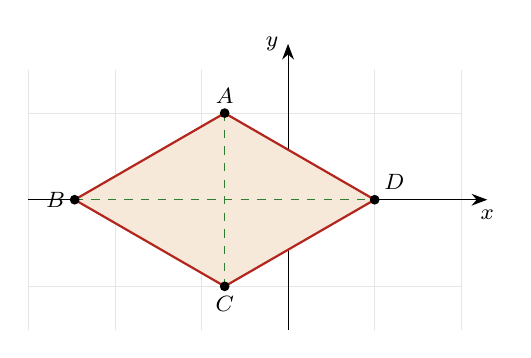
\begin{tikzpicture}[scale=1.1,font=\footnotesize]
\draw[gray!20,very thin](-3,-1.5) grid (2,1.5);
\draw[-{Stealth[length=2mm]}](-3,0)--(2.3,0) node[below]{$x$};
\draw[-{Stealth[length=2mm]}](0,-1.5)--(0,1.8) node[left]{$y$};
\node[below right] at (0,0){$O$};
\fill[cEx!15](-0.732,1)--(-2.464,0)--(-0.732,-1)--(1,0)--cycle;
\draw[cThm,thick](-0.732,1)--(-2.464,0)--(-0.732,-1)--(1,0)--cycle;
\draw[cRem,dashed](-0.732,1)--(-0.732,-1) (-2.464,0)--(1,0);
\fill (-0.732,1) circle (1.6pt) node[above]{$A$};
\fill (-2.464,0) circle (1.6pt) node[left]{$B$};
\fill (-0.732,-1) circle (1.6pt) node[below]{$C$};
\fill (1,0) circle (1.6pt) node[above right]{$D$};
\end{tikzpicture}\end{LTR}\end{center}
\end{hal}
% ===================== التمرين 6 =====================
\Needspace{12\baselineskip}
\begin{tamrin}{بكالوريا 2024 -- الموضوع الثاني -- علوم تجريبية}
عين الاقتراح الصحيح الوحيد من بين الاقتراحات الثلاثة مع التبرير في كل حالة مما يلي:
\QQ{1} $z$ عدد مركب مرافقه $\overline{z}$. مرافق العدد المركب $z+i$ هو:
\ABC{$\overline{z}-i$}{$\overline{z}+i$}{$z-i$}
\QQ{2} العدد المركب $\left(\dfrac{1+i}{1-i}\right)^{2024}$ يساوي:
\ABC{$1$}{$i$}{$-1$}
\QQ{3} $z$ عدد مركب حيث $z=2\left(1+i\sqrt3\right)$.
من أجل كل عدد طبيعي غير معدوم $n$، نضع: $S_n=\ln|z|+\ln|z|^2+\ldots+\ln|z|^n$، لدينا:
\begin{sq}
\qa $S_n=(n+1)^2\ln2$ \qquad\qquad (ب) $S_n=n(n+1)\ln2$
\qc $S_n=2\left(\dfrac{1-(2\ln2)^n}{1-2\ln2}\right)\ln2$
\end{sq}
\QQ{4} $z$ عدد مركب حيث: $z=\sin\dfrac{\pi}{8}+i\cos\dfrac{\pi}{8}$. الشكل المثلثي للعدد المركب $z$ هو:
\ABC{$z=-\cos\dfrac{\pi}{8}+i\sin\dfrac{\pi}{8}$}{$z=\cos\dfrac{\pi}{8}+i\sin\dfrac{\pi}{8}$}{$z=\cos\dfrac{3\pi}{8}+i\sin\dfrac{3\pi}{8}$}
\end{tamrin}

\begin{hal}
\QQ{1} مرافق مجموع هو مجموع المرافقين: $\overline{z+i}=\overline{z}+\overline{i}=\overline{z}-i$.
الاقتراح الصحيح: \bxt{(أ) $\overline{z}-i$}.

\QQ{2} $\dfrac{1+i}{1-i}=\dfrac{(1+i)^2}{(1-i)(1+i)}=\dfrac{2i}{2}=i$، ومنه $\left(\dfrac{1+i}{1-i}\right)^{2024}=i^{2024}=\left(i^4\right)^{506}=1$ (لأن $2024=4\times506$).
الاقتراح الصحيح: \bxt{(أ) $1$}.

\QQ{3} $|z|=2\sqrt{1+3}=4$. لدينا $\ln|z|^k=k\ln4=2k\ln2$، إذن
\[S_n=2\ln2\,(1+2+\ldots+n)=2\ln2\times\frac{n(n+1)}{2}=n(n+1)\ln2 .\]
الاقتراح الصحيح: \bxt{(ب) $S_n=n(n+1)\ln2$}.

\QQ{4} نستعمل $\sin x=\cos\left(\frac{\pi}{2}-x\right)$ و$\cos x=\sin\left(\frac{\pi}{2}-x\right)$:
\[z=\cos\left(\frac{\pi}{2}-\frac{\pi}{8}\right)+i\sin\left(\frac{\pi}{2}-\frac{\pi}{8}\right)=\cos\frac{3\pi}{8}+i\sin\frac{3\pi}{8}.\]
الاقتراح الصحيح: \bxt{(جـ) $z=\cos\frac{3\pi}{8}+i\sin\frac{3\pi}{8}$}.
(الاقتراح (أ) ليس شكلا مثلثيا، والاقتراح (ب) يعطي $\cos\frac{\pi}{8}\neq\sin\frac{\pi}{8}$.)
\end{hal}

% ===================== التمرين 7 =====================
\Needspace{12\baselineskip}
\begin{tamrin}{بكالوريا 2023 -- الموضوع الثاني -- علوم تجريبية}
عين الاقتراح الصحيح الوحيد من بين الاقتراحات الثلاثة في كل حالة من الحالات التالية مع التبرير:
\QQ{1} حلا المعادلة $8z^2-4z+1=0$ ذات المجهول $z$ في $\mathbb{C}$ هما:
\ABC{$-\frac14+\frac14i$ و$\frac14-\frac14i$}{$-\frac14+\frac14i$ و$-\frac14-\frac14i$}{$\frac14-\frac14i$ و$\frac14+\frac14i$}
\QQ{2} الشكل الجبري للعدد المركب $\dfrac{1+\sqrt3+i}{1-i}$ هو:
\ABC{$\dfrac{\sqrt3}{2}+i\left(\dfrac{2+\sqrt3}{2}\right)$}{$\dfrac{\sqrt3}{2}-i\left(\dfrac{2+\sqrt3}{2}\right)$}{$\dfrac{\sqrt3}{2}+i\left(\dfrac{-2+\sqrt3}{2}\right)$}
\QQ{3} الجذران التربيعيان للعدد المركب $-8+6i$ هما:
\ABC{$1+3i$ و$-1-3i$}{$1+3i$ و$1-3i$}{$3+i$ و$-3-i$}
\QQ{4} الشكل المثلثي للعدد المركب $\dfrac{1+i}{\sqrt3-i}$ هو:
\ABC{$\sqrt2\left(\cos\frac{\pi}{12}+i\sin\frac{\pi}{12}\right)$}{$\frac{\sqrt2}{2}\left(\cos\frac{5\pi}{12}+i\sin\frac{5\pi}{12}\right)$}{$\frac{\sqrt2}{2}\left(\cos\frac{7\pi}{12}+i\sin\frac{7\pi}{12}\right)$}
\end{tamrin}

\begin{hal}
\QQ{1} $\Delta=(-4)^2-4\times8\times1=16-32=-16=(4i)^2$، إذن
$z_1=\dfrac{4-4i}{16}=\dfrac14-\dfrac14i$ و$z_2=\dfrac{4+4i}{16}=\dfrac14+\dfrac14i$.
الاقتراح الصحيح: \bxt{(جـ)}.

\QQ{2} نضرب البسط والمقام في مرافق المقام $1+i$:
\[\frac{\left(1+\sqrt3+i\right)(1+i)}{(1-i)(1+i)}=\frac{1+\sqrt3+i\left(1+\sqrt3\right)+i-1}{2}=\frac{\sqrt3+i\left(2+\sqrt3\right)}{2}.\]
الاقتراح الصحيح: \bxt{(أ) $\frac{\sqrt3}{2}+i\left(\frac{2+\sqrt3}{2}\right)$}.

\QQ{3} $(1+3i)^2=1+6i+9i^2=-8+6i$، إذن الجذران التربيعيان هما $1+3i$ و$-(1+3i)=-1-3i$.
الاقتراح الصحيح: \bxt{(أ)}.
(تحقق: $(1-3i)^2=-8-6i$ و$(3+i)^2=8+6i$.)

\QQ{4} $1+i=\sqrt2\left(\cos\frac{\pi}{4}+i\sin\frac{\pi}{4}\right)$ و$\sqrt3-i=2\left(\cos\left(-\frac{\pi}{6}\right)+i\sin\left(-\frac{\pi}{6}\right)\right)$، إذن
\[\left|\frac{1+i}{\sqrt3-i}\right|=\frac{\sqrt2}{2},\qquad \arg\frac{1+i}{\sqrt3-i}=\frac{\pi}{4}+\frac{\pi}{6}=\frac{5\pi}{12}.\]
الاقتراح الصحيح: \bxt{(ب) $\frac{\sqrt2}{2}\left(\cos\frac{5\pi}{12}+i\sin\frac{5\pi}{12}\right)$}.
\end{hal}

% ===================== التمرين 8 =====================
\Needspace{12\baselineskip}
\begin{tamrin}{بكالوريا 2019 -- الموضوع الأول -- علوم تجريبية}
\textbf{I)} حل في المجموعة $\mathbb{C}$ المعادلة: $(z-i)\left(z^2-4z+5\right)=0$.

\textbf{II)} نعتبر في المستوي المنسوب إلى المعلم المتعامد والمتجانس $(O;\vec u,\vec v)$ النقط $A$، $B$ و$C$ التي لاحقاتها: $i$، $2-i$ و$2+i$ على الترتيب.
\QQ{1} أكتب العدد المركب $\dfrac{z_C-z_A}{z_C-z_B}$ على الشكل الأسي، ثم استنتج طبيعة المثلث $ABC$.
\QQ{2} من أجل كل عدد مركب $z$ يختلف عن $2+i$ نضع: $f(z)=\dfrac{iz-1-2i}{2z-4-2i}$.
\begin{sq}
\qa عين المجموعة $(E)$ للنقط $M$ من المستوي ذات اللاحقة $z$ والتي تحقق $|f(z)|=\dfrac12$.
\qb بين أن العدد $\left[f(i)\right]^{1440}$ حقيقي موجب.
\end{sq}
\QQ{3} نعتبر الدوران $r$ الذي مركزه النقطة $C$ وزاويته $\dfrac{\pi}{2}$.
\begin{sq}
\qa عين لاحقة النقطة $D$ صورة النقطة $B$ بالدوران $r$، وبين أن النقط $A$، $D$ و$C$ في استقامية.
\qb استنتج أن النقطة $D$ هي صورة النقطة $A$ بتحويل نقطي بسيط يطلب تعيين عناصره المميزة.
\end{sq}
\end{tamrin}

\begin{hal}
\textbf{I)} $z-i=0$ يعني $z=i$. و$z^2-4z+5=0$: $\Delta=16-20=-4=(2i)^2$ ومنه $z=\dfrac{4\pm2i}{2}=2\pm i$.
\bx{S=\{i\,;\,2-i\,;\,2+i\}}.

\textbf{II)}
\QQ{1} $\dfrac{z_C-z_A}{z_C-z_B}=\dfrac{2+i-i}{2+i-2+i}=\dfrac{2}{2i}=\dfrac1i=-i$، إذن \bx{\frac{z_C-z_A}{z_C-z_B}=e^{-i\frac{\pi}{2}}}.

ومنه $\dfrac{CA}{CB}=1$ أي $CA=CB$، و$\left(\overrightarrow{CB},\overrightarrow{CA}\right)=-\dfrac{\pi}{2}$ أي $(CA)\perp(CB)$:
\bxt{المثلث $ABC$ قائم ومتساوي الساقين في $C$}.

\QQ{2}
\pa نلاحظ أن $iz-1-2i=i\left(z-\dfrac{1+2i}{i}\right)=i\left(z-(2-i)\right)=i(z-z_B)$ و$2z-4-2i=2(z-z_C)$، إذن من أجل $z\neq z_C$:
\[f(z)=\frac{i\,(z-z_B)}{2\,(z-z_C)}\quad\Longrightarrow\quad|f(z)|=\frac{|i|\,|z-z_B|}{2\,|z-z_C|}=\frac{MB}{2\,MC}.\]
$|f(z)|=\dfrac12$ يعني $\dfrac{MB}{2MC}=\dfrac12$ أي $MB=MC$: $M$ متساوية البعد عن $B$ و$C$.
إذن \bxt{$(E)$ هي محور القطعة $[BC]$}. بما أن $B(2;-1)$ و$C(2;1)$ فمنتصف $[BC]$ هو $(2;0)$ و$(BC)$ شاقولي، إذن $(E)$ هو المستقيم \bx{y=0} أي \bxt{محور الفواصل}.

\pb $f(i)=\dfrac{i^2-1-2i}{2i-4-2i}=\dfrac{-2-2i}{-4}=\dfrac{1+i}{2}=\dfrac{\sqrt2}{2}e^{i\frac{\pi}{4}}$، ومنه
\[\left[f(i)\right]^{1440}=\left(\frac{\sqrt2}{2}\right)^{1440}e^{i\frac{1440\pi}{4}}=\left(\frac12\right)^{720}e^{i\,360\pi}=\left(\frac12\right)^{720}.\]
لأن $360\pi=180\times2\pi$. إذن \bx{\left[f(i)\right]^{1440}=\frac{1}{2^{720}}>0}: عدد حقيقي موجب.

\QQ{3} العبارة المركبة للدوران $r$: $z'-z_C=e^{i\frac{\pi}{2}}(z-z_C)$ أي $z'=iz+3-i$ (لأن $z_C-iz_C=2+i-2i+1=3-i$).
\pa $z_D=i(z_B-z_C)+z_C=i(-2i)+2+i=2+2+i$ أي \bx{z_D=4+i}.

$\dfrac{z_D-z_A}{z_C-z_A}=\dfrac{4}{2}=2\in\mathbb{R}$، إذن $\overrightarrow{AD}=2\overrightarrow{AC}$: النقط $A$، $C$ و$D$ في استقامية (كلها على المستقيم $y=1$).

\pb من $\overrightarrow{AD}=2\overrightarrow{AC}$ نستنتج أن $C$ منتصف $[AD]$ (تحقق: $\frac{z_A+z_D}{2}=\frac{4+2i}{2}=2+i=z_C$).
إذن \bxt{$D$ صورة $A$ بالتناظر المركزي الذي مركزه $C$}، عبارته $z'=-z+2z_C=-z+4+2i$ (وهو الدوران الذي مركزه $C$ وزاويته $\pi$).
(ملاحظة: بما أن $z_D-z_A=4$ فإن $D$ هي أيضا صورة $A$ بالانسحاب الذي شعاعه $\vec w$ ذو اللاحقة $4$.)

\begin{center}\begin{LTR}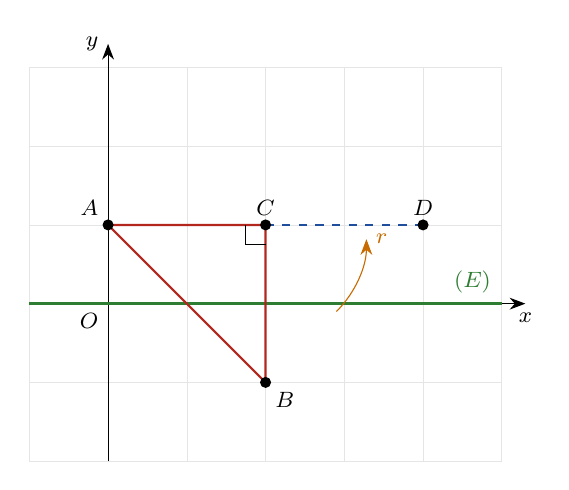
\begin{tikzpicture}[scale=1,font=\footnotesize]
\draw[gray!20,very thin](-1,-2) grid (5,3);
\draw[-{Stealth[length=2mm]}](-1,0)--(5.3,0) node[below]{$x$};
\draw[-{Stealth[length=2mm]}](0,-2)--(0,3.3) node[left]{$y$};
\node[below left] at (0,0){$O$};
\draw[cRem,very thick](-1,0)--(5,0) node[above left]{$(E)$};
\draw[cThm,thick](0,1)--(2,-1)--(2,1)--cycle;
\draw[cDef,thick,dashed](2,1)--(4,1);
\draw (2,1)++(-0.25,0)--++(0,-0.25)--++(0.25,0);
\draw[-{Stealth[length=2mm]},cEx](2.9,-0.1) arc (-45:0:1.3) node[right]{$r$};
\fill (0,1) circle (2pt) node[above left]{$A$};
\fill (2,-1) circle (2pt) node[below right]{$B$};
\fill (2,1) circle (2pt) node[above]{$C$};
\fill (4,1) circle (2pt) node[above]{$D$};
\end{tikzpicture}\end{LTR}\end{center}
\end{hal}

% ===================== التمرين 9 =====================
\Needspace{12\baselineskip}
\begin{tamrin}{بكالوريا 2019 -- الموضوع الثاني -- علوم تجريبية}
المستوي منسوب إلى المعلم المتعامد والمتجانس $(O;\vec u,\vec v)$.
نعتبر النقط $A$، $B$ و$C$ التي لاحقاتها $z_A$، $z_B$ و$z_C$ على الترتيب حيث: $z_A=\sqrt2+i\sqrt6$، $z_B=\overline{z_A}$ و$z_C=-2z_A$.
\QQ{1}
\begin{sq}
\qa أكتب العدد المركب $z_A$ على الشكل الأسي.
\qb أحسب العدد $\left(\dfrac{z_A}{2\sqrt2}\right)^{2019}+\left(\dfrac{z_B}{2\sqrt2}\right)^{2019}$.
\end{sq}
\QQ{2}
\begin{sq}
\qa $T$ الانسحاب الذي يحول $A$ إلى $C$. عين $z_D$ لاحقة النقطة $D$ صورة النقطة $B$ بالانسحاب $T$.
\qb استنتج طبيعة الرباعي $ABDC$.
\end{sq}
\QQ{3} أكتب العدد المركب $z_C-z_A$ على الشكل الأسي.
\QQ{4} جد قيم العدد الطبيعي $n$ التي يكون من أجلها العدد المركب $\left(\dfrac{-6\sqrt2}{z_C-z_A}\right)^n$ عددا حقيقيا.
\QQ{5} لتكن $M$ نقطة كيفية من المستوي لاحقتها $z$ تختلف عن $A$ وتختلف عن $C$.
عين $(E)$ مجموعة النقط $M$ التي يكون من أجلها $\dfrac{z_A-z}{z_C-z}$ عددا حقيقيا موجبا تماما.
\end{tamrin}

\begin{hal}
\QQ{1}
\pa $|z_A|=\sqrt{2+6}=2\sqrt2$، $\cos\theta=\dfrac{\sqrt2}{2\sqrt2}=\dfrac12$ و$\sin\theta=\dfrac{\sqrt6}{2\sqrt2}=\dfrac{\sqrt3}{2}$ إذن $\theta=\dfrac{\pi}{3}$:
\bx{z_A=2\sqrt2\,e^{i\frac{\pi}{3}}}.

\pb $\dfrac{z_A}{2\sqrt2}=e^{i\frac{\pi}{3}}$ و$\dfrac{z_B}{2\sqrt2}=\overline{\left(\dfrac{z_A}{2\sqrt2}\right)}=e^{-i\frac{\pi}{3}}$، ومنه (دستور موافر):
\[e^{i\frac{2019\pi}{3}}+e^{-i\frac{2019\pi}{3}}=2\cos\frac{2019\pi}{3}=2\cos(673\pi)=2\cos(\pi+336\times2\pi)=2\cos\pi .\]
إذن \bx{\left(\frac{z_A}{2\sqrt2}\right)^{2019}+\left(\frac{z_B}{2\sqrt2}\right)^{2019}=-2}.

\QQ{2}
\pa شعاع الانسحاب $T$ هو $\overrightarrow{AC}$ ولاحقته $z_C-z_A=-3z_A=-3\sqrt2-3i\sqrt6$.
$T(B)=D$ يعني $z_D=z_B+z_C-z_A=\sqrt2-i\sqrt6-3\sqrt2-3i\sqrt6$ أي \bx{z_D=-2\sqrt2-4i\sqrt6}.

\pb $\overrightarrow{BD}=\overrightarrow{AC}$ إذن $ABDC$ متوازي أضلاع.
ليس معينا لأن $AB=|z_B-z_A|=|-2i\sqrt6|=2\sqrt6$ و$AC=|-3z_A|=6\sqrt2$ (ضلعان متتاليان غير متقايسين)، وليس مستطيلا لأن $\dfrac{z_C-z_A}{z_B-z_A}=\dfrac{3}{2}-\dfrac{\sqrt3}{2}i$ ليس تخيليا صرفا.
إذن \bxt{$ABDC$ متوازي أضلاع}.

\QQ{3} $z_C-z_A=-3z_A=3\times2\sqrt2\,e^{i\pi}e^{i\frac{\pi}{3}}=6\sqrt2\,e^{i\frac{4\pi}{3}}$، أي \bx{z_C-z_A=6\sqrt2\,e^{-i\frac{2\pi}{3}}}.

\QQ{4} $\dfrac{-6\sqrt2}{z_C-z_A}=\dfrac{6\sqrt2\,e^{i\pi}}{6\sqrt2\,e^{-i\frac{2\pi}{3}}}=e^{i\frac{5\pi}{3}}=e^{-i\frac{\pi}{3}}$، ومنه $\left(\dfrac{-6\sqrt2}{z_C-z_A}\right)^n=e^{-i\frac{n\pi}{3}}$.

يكون حقيقيا إذا وفقط إذا كان $\sin\left(-\dfrac{n\pi}{3}\right)=0$ أي $\dfrac{n\pi}{3}=k\pi$ أي $n=3k$:
\bxt{$n=3k$ مع $k\in\mathbb{N}$}.

\QQ{5} $\dfrac{z_A-z}{z_C-z}$ هو نسبة لاحقتي الشعاعين $\overrightarrow{MA}$ و$\overrightarrow{MC}$. يكون حقيقيا موجبا تماما إذا وفقط إذا كان
$\arg\left(\dfrac{z_A-z}{z_C-z}\right)=0+2k\pi$ أي $\left(\overrightarrow{MC},\overrightarrow{MA}\right)=0+2k\pi$:
الشعاعان $\overrightarrow{MA}$ و$\overrightarrow{MC}$ مرتبطان خطيا ولهما نفس الاتجاه، أي $M\in(AC)$ و$M\notin[AC]$.

إذن \bxt{$(E)$ هي المستقيم $(AC)$ محروما من القطعة $[AC]$}.
(بما أن $z_C=-2z_A$ فإن $(AC)$ يشمل $O$، معادلته $y=\sqrt3\,x$.)

\begin{center}\begin{LTR}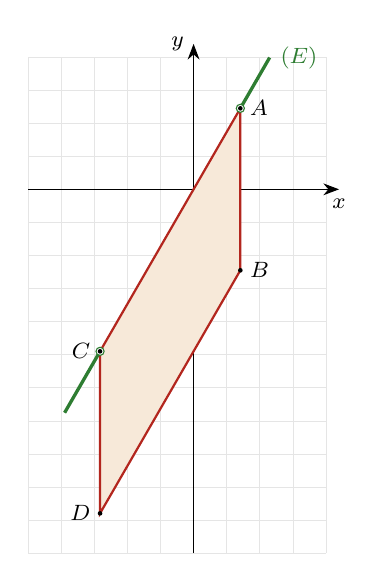
\begin{tikzpicture}[scale=0.42,font=\footnotesize]
\draw[gray!20,very thin](-5,-11) grid (4,4);
\draw[-{Stealth[length=2mm]}](-5,0)--(4.4,0) node[below]{$x$};
\draw[-{Stealth[length=2mm]}](0,-11)--(0,4.4) node[left]{$y$};
\node[below right] at (0,0){$O$};
\draw[gray,dashed](1.414,2.449)--(-2.828,-4.899);
\draw[cRem,very thick](1.414,2.449)--(2.3,3.984) node[right]{$(E)$};
\draw[cRem,very thick](-2.828,-4.899)--(-3.9,-6.755);
\fill[cEx!15](1.414,2.449)--(1.414,-2.449)--(-2.828,-9.798)--(-2.828,-4.899)--cycle;
\draw[cThm,thick](1.414,2.449)--(1.414,-2.449)--(-2.828,-9.798)--(-2.828,-4.899)--cycle;
\draw[cRem,fill=white] (1.414,2.449) circle (3.5pt);
\draw[cRem,fill=white] (-2.828,-4.899) circle (3.5pt);
\fill (1.414,2.449) circle (2pt) node[right]{$A$};
\fill (1.414,-2.449) circle (2pt) node[right]{$B$};
\fill (-2.828,-4.899) circle (2pt) node[left]{$C$};
\fill (-2.828,-9.798) circle (2pt) node[left]{$D$};
\end{tikzpicture}\end{LTR}\end{center}
\end{hal}

% ===================== التمرين 10 =====================
\Needspace{12\baselineskip}
\begin{tamrin}{بكالوريا 2018 -- الموضوع الأول -- علوم تجريبية}
\QQ{1} حل في مجموعة الأعداد المركبة $\mathbb{C}$ المعادلة ذات المجهول $z$ التالية: $z^2-\sqrt3\,z+1=0$.
\QQ{2} المستوي المركب منسوب إلى المعلم المتعامد والمتجانس $(O;\vec u,\vec v)$. $A$، $B$ و$C$ ثلاث نقط من المستوي لواحقها على الترتيب: $z_A=\dfrac12+i\dfrac{\sqrt3}{2}$، $z_B=\dfrac{\sqrt3}{2}+\dfrac12i$ و$z_C=\overline{z_B}$.

أكتب $z_A$ و$z_B$ على الشكل الأسي ثم عين قيم العدد الطبيعي $n$ بحيث يكون: $\left(\dfrac{z_A}{z_B}\right)^n=\dfrac{1+i\sqrt3}{2}$.
\QQ{3}
\begin{sq}
\qa تحقق أن: $\dfrac{z_B}{z_C}=e^{i\frac{\pi}{3}}$ وحدد طبيعة المثلث $OBC$.
\qb استنتج أن $B$ هي صورة $C$ بدوران $r$ يطلب تعيين عناصره المميزة.
\end{sq}
\QQ{4} نسمي $(\gamma)$ مجموعة النقط $M$ ذات اللاحقة $z$ التي تحقق: $|z|=\left|\overline{z}-\dfrac{\sqrt3+i}{2}\right|$.
عين طبيعة المجموعة $(\gamma)$ ثم عين صورتها بالدوران $r$.
\end{tamrin}

\begin{hal}
\QQ{1} $\Delta=3-4=-1=i^2$، إذن $z_1=\dfrac{\sqrt3-i}{2}$ و$z_2=\dfrac{\sqrt3+i}{2}$:
\bx{S=\left\{\frac{\sqrt3}{2}-\frac12i\,;\,\frac{\sqrt3}{2}+\frac12i\right\}}.

\QQ{2} $|z_A|=\sqrt{\frac14+\frac34}=1$ و$\cos\theta=\frac12$، $\sin\theta=\frac{\sqrt3}{2}$: \bx{z_A=e^{i\frac{\pi}{3}}}.
$|z_B|=1$ و$\cos\theta=\frac{\sqrt3}{2}$، $\sin\theta=\frac12$: \bx{z_B=e^{i\frac{\pi}{6}}}.

$\dfrac{z_A}{z_B}=e^{i\left(\frac{\pi}{3}-\frac{\pi}{6}\right)}=e^{i\frac{\pi}{6}}$، و$\dfrac{1+i\sqrt3}{2}=z_A=e^{i\frac{\pi}{3}}$. إذن:
\[\left(\frac{z_A}{z_B}\right)^n=\frac{1+i\sqrt3}{2}\iff e^{i\frac{n\pi}{6}}=e^{i\frac{\pi}{3}}\iff\frac{n\pi}{6}=\frac{\pi}{3}+2k\pi\iff n=2+12k .\]
\bxt{$n=12k+2$ مع $k\in\mathbb{N}$}.

\QQ{3}
\pa $z_C=\overline{z_B}=e^{-i\frac{\pi}{6}}$ إذن $\dfrac{z_B}{z_C}=e^{i\left(\frac{\pi}{6}+\frac{\pi}{6}\right)}=e^{i\frac{\pi}{3}}$ \ok.

ومنه $\dfrac{OB}{OC}=1$ و$\left(\overrightarrow{OC},\overrightarrow{OB}\right)=\dfrac{\pi}{3}$: مثلث متساوي الساقين رأسه $O$ وزاويته $\frac{\pi}{3}$،
إذن \bxt{المثلث $OBC$ متقايس الأضلاع}.

\pb $z_B=e^{i\frac{\pi}{3}}z_C$ هي من الشكل $z'=e^{i\frac{\pi}{3}}z$:
\bxt{$B=r(C)$ حيث $r$ الدوران الذي مركزه $O$ وزاويته $\frac{\pi}{3}$}.

\QQ{4} $\left|\overline{z}-\dfrac{\sqrt3+i}{2}\right|=\left|\overline{z}-z_B\right|=\left|\overline{z-\overline{z_B}}\right|=|z-z_C|$ (لأن $|\overline{w}|=|w|$).

إذن $|z|=|z-z_C|$ تعني $OM=CM$:
\bxt{$(\gamma)$ هي محور القطعة $[OC]$}، معادلته $\sqrt3\,x-y-1=0$.

صورة $(\gamma)$ بالدوران $r$: الدوران يحفظ المسافات، و$r(O)=O$، $r(C)=B$، إذن صورة محور $[OC]$ هي محور $[OB]$:
\bxt{$r(\gamma)$ هي محور القطعة $[OB]$} ومعادلته $\sqrt3\,x+y-1=0$.

\begin{center}\begin{LTR}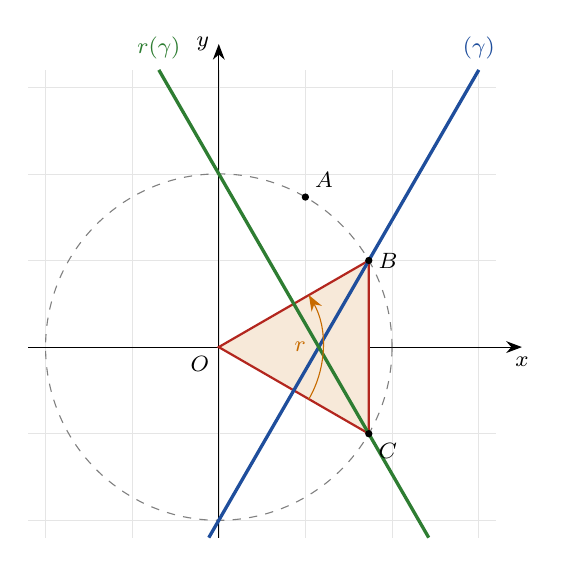
\begin{tikzpicture}[scale=2.2,font=\footnotesize]
\draw[gray!20,very thin,step=0.5](-1.1,-1.1) grid (1.6,1.6);
\draw[-{Stealth[length=2mm]}](-1.1,0)--(1.75,0) node[below]{$x$};
\draw[-{Stealth[length=2mm]}](0,-1.1)--(0,1.75) node[left]{$y$};
\node[below left] at (0,0){$O$};
\draw[gray,dashed](0,0) circle (1);
\fill[cEx!15](0,0)--(0.866,0.5)--(0.866,-0.5)--cycle;
\draw[cThm,thick](0,0)--(0.866,0.5)--(0.866,-0.5)--cycle;
\draw[cDef,very thick](-0.0577,-1.1)--(1.501,1.6) node[above]{$(\gamma)$};
\draw[cRem,very thick](-0.346,1.6) node[above]{$r(\gamma)$}--(1.212,-1.1);
\draw[-{Stealth[length=2mm]},cEx](0.52,-0.3) arc (-30:30:0.6);
\node[cEx] at (0.47,0){$r$};
\fill (0.5,0.866) circle (0.6pt) node[above right]{$A$};
\fill (0.866,0.5) circle (0.6pt) node[right]{$B$};
\fill (0.866,-0.5) circle (0.6pt) node[below right]{$C$};
\end{tikzpicture}\end{LTR}\end{center}
\end{hal}
% ===================== التمرين 11 =====================
\Needspace{12\baselineskip}
\begin{tamrin}{بكالوريا 2018 -- الموضوع الثاني -- علوم تجريبية}
\textbf{I)} حل في مجموعة الأعداد المركبة $\mathbb{C}$ المعادلة: $\left(\overline{z}-4+i\right)\left(z^2-4z+5\right)=0$ (يرمز $\overline{z}$ لمرافق العدد $z$).

\textbf{II)} في المستوي المركب المنسوب إلى المعلم المتعامد والمتجانس $(O;\vec u,\vec v)$، نعتبر النقط $A$، $B$ و$C$ لواحقها على الترتيب: $z_A=2+i$، $z_B=4+i$ و$z_C=\overline{z_A}$.
\QQ{1} تحقق أن: $\dfrac{z_B-z_A}{z_C-z_A}=i$، ثم عين قيم العدد الطبيعي $n$ بحيث يكون $\left(\dfrac{z_B-z_A}{z_C-z_A}\right)^n$ تخيليا صرفا.
\QQ{2} $D$ نقطة من المستوي لاحقتها $z_D$ حيث:
$\begin{cases}|z_D-z_A|=|z_B-z_A|\\[2pt] \arg\left(\dfrac{z_D-z_A}{z_B-z_A}\right)=\dfrac{\pi}{3}+2k\pi\quad(k\in\mathbb{Z})\end{cases}$

بين أن المثلث $ABD$ متقايس الأضلاع وأحسب $z_D$.
\QQ{3} أحسب $z_G$ لاحقة النقطة $G$ مركز ثقل المثلث $ABD$ ثم عين نسبة وزاوية التشابه المباشر الذي مركزه $A$ ويحول $G$ إلى $D$.
\QQ{4} عين $(\Gamma)$ مجموعة النقط $M$ ذات اللاحقة $z$ ($M$ تختلف عن $C$) بحيث: $\arg\left(\dfrac{z_G-z}{z_C-z}\right)=\pi+2k\pi$ ($k\in\mathbb{Z}$).
\end{tamrin}

\begin{hal}
\textbf{I)} $\overline{z}-4+i=0$ يعني $\overline{z}=4-i$ أي $z=4+i$.
و$z^2-4z+5=0$: $\Delta=16-20=-4=(2i)^2$ ومنه $z=2-i$ أو $z=2+i$.
\bx{S=\{4+i\,;\,2-i\,;\,2+i\}}.

\textbf{II)}
\QQ{1} $z_C=2-i$. $\dfrac{z_B-z_A}{z_C-z_A}=\dfrac{2}{-2i}=\dfrac{-1}{i}=i$ \ok. إذن \bx{\frac{z_B-z_A}{z_C-z_A}=i=e^{i\frac{\pi}{2}}}.

$i^n=e^{i\frac{n\pi}{2}}$ تخيلي صرف إذا وفقط إذا كان $\cos\dfrac{n\pi}{2}=0$ أي $\dfrac{n\pi}{2}=\dfrac{\pi}{2}+k\pi$ أي $n=2k+1$:
\bxt{$n$ فردي: $n=2k+1$ مع $k\in\mathbb{N}$}.

\QQ{2} $|z_D-z_A|=|z_B-z_A|$ يعني $AD=AB$، و$\arg\left(\dfrac{z_D-z_A}{z_B-z_A}\right)=\dfrac{\pi}{3}$ يعني $\left(\overrightarrow{AB},\overrightarrow{AD}\right)=\dfrac{\pi}{3}$.
المثلث $ABD$ متساوي الساقين رأسه $A$ وزاويته الرئيسية $\frac{\pi}{3}$، إذن \bxt{$ABD$ متقايس الأضلاع}.

من المعطيين: $\dfrac{z_D-z_A}{z_B-z_A}=1\times e^{i\frac{\pi}{3}}$، ومنه
\[z_D=z_A+e^{i\frac{\pi}{3}}(z_B-z_A)=2+i+2\left(\frac12+i\frac{\sqrt3}{2}\right)\]
\bx{z_D=3+i\left(1+\sqrt3\right)}.

\QQ{3} $z_G=\dfrac{z_A+z_B+z_D}{3}=\dfrac{2+i+4+i+3+i+i\sqrt3}{3}=\dfrac{9+i\left(3+\sqrt3\right)}{3}$ أي \bx{z_G=3+i\left(1+\frac{\sqrt3}{3}\right)}.

التشابه المباشر $S$ الذي مركزه $A$ ويحول $G$ إلى $D$ عبارته $z'-z_A=a(z-z_A)$ حيث
\[a=\frac{z_D-z_A}{z_G-z_A}=\frac{1+i\sqrt3}{1+i\frac{\sqrt3}{3}}=\frac{3\left(1+i\sqrt3\right)}{3+i\sqrt3}=\frac{3\left(1+i\sqrt3\right)\left(3-i\sqrt3\right)}{12}=\frac{3\left(6+2i\sqrt3\right)}{12}=\frac32+\frac{\sqrt3}{2}i .\]
$|a|=\sqrt{\frac94+\frac34}=\sqrt3$ و$a=\sqrt3\left(\frac{\sqrt3}{2}+\frac12i\right)=\sqrt3\,e^{i\frac{\pi}{6}}$.
إذن \bxt{نسبة $S$ هي $\sqrt3$ وزاويته $\frac{\pi}{6}$}.
(تفسير: في المثلث المتقايس الأضلاع $AD=\sqrt3\,AG$، و$(AG)$ منصف الزاوية $\widehat{BAD}$.)

\QQ{4} $\arg\left(\dfrac{z_G-z}{z_C-z}\right)=\pi+2k\pi$ يعني $\left(\overrightarrow{MC},\overrightarrow{MG}\right)=\pi$: الشعاعان $\overrightarrow{MG}$ و$\overrightarrow{MC}$ مرتبطان خطيا ومتعاكسان في الاتجاه، أي $M$ تقع بين $G$ و$C$ (مع $M\neq G$ و$M\neq C$).
إذن \bxt{$(\Gamma)$ هي القطعة $[GC]$ محرومة من طرفيها $G$ و$C$}.

\begin{center}\begin{LTR}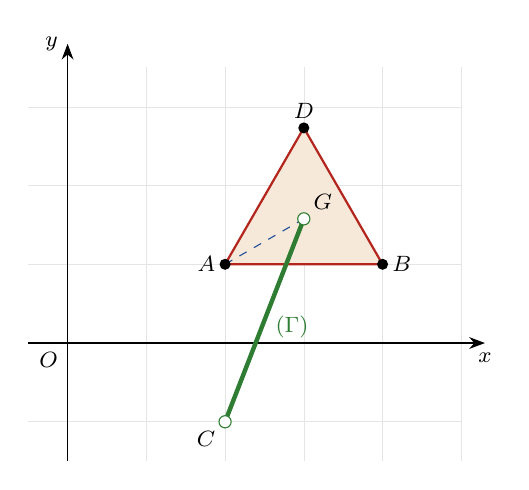
\begin{tikzpicture}[scale=1,font=\footnotesize]
\draw[gray!20,very thin](-0.5,-1.5) grid (5,3.5);
\draw[-{Stealth[length=2mm]}](-0.5,0)--(5.3,0) node[below]{$x$};
\draw[-{Stealth[length=2mm]}](0,-1.5)--(0,3.8) node[left]{$y$};
\node[below left] at (0,0){$O$};
\fill[cEx!15](2,1)--(4,1)--(3,2.732)--cycle;
\draw[cThm,thick](2,1)--(4,1)--(3,2.732)--cycle;
\draw[cDef,dashed](2,1)--(3,1.577);
\draw[cRem,line width=1.6pt](3,1.577)--(2,-1);
\node[cRem] at (2.85,0.2){$(\Gamma)$};
\draw[cRem,fill=white](3,1.577) circle (2.2pt);
\draw[cRem,fill=white](2,-1) circle (2.2pt);
\fill (2,1) circle (2pt) node[left]{$A$};
\fill (4,1) circle (2pt) node[right]{$B$};
\fill (3,2.732) circle (2pt) node[above]{$D$};
\node[above right] at (3,1.577){$G$};
\node[below left] at (2,-1){$C$};
\end{tikzpicture}\end{LTR}\end{center}
\end{hal}

% ===================== التمرين 12 =====================
\Needspace{12\baselineskip}
\begin{tamrin}{بكالوريا 2017 -- الدورة الاستثنائية -- الموضوع الأول -- علوم تجريبية}
\textbf{I)} حل في المجموعة $\mathbb{C}$ المعادلة: $(z-2)\left(z^2+2z+4\right)=0$.

\textbf{II)} المستوي المركب منسوب إلى المعلم المتعامد والمتجانس $(O;\vec u,\vec v)$ حيث $\|\vec u\|=2\,\text{cm}$.
نعتبر النقط $A$، $B$ و$C$ التي لاحقاتها: $z_A=2$، $z_B=-1+i\sqrt3$ و$z_C=\overline{z_B}$.
\QQ{1}
\begin{sq}
\qa أكتب $z_B$ على الشكل الأسي، ثم استنتج الشكل الأسي للعدد المركب $z_C$.
\qb عين مركز ونصف قطر الدائرة المحيطة بالمثلث $ABC$، ثم أنشئ النقط $A$، $B$ و$C$.
\end{sq}
\QQ{2} ليكن $S$ التشابه المباشر الذي مركزه النقطة $O$ ونسبته $\dfrac12$ وزاويته $\dfrac{2\pi}{3}$ ولتكن $F$ صورة $A$ بالتحويل $S$.
\begin{sq}
\qa أكتب العبارة المركبة للتشابه $S$ ثم عين لاحقة كل من $A'$، $B'$ و$C'$ صور النقط $A$، $B$ و$C$ على الترتيب بالتشابه $S$، ثم أنشئ في المعلم السابق النقط $A'$، $B'$ و$C'$.
\qb أحسب بالسنتيمتر المربع مساحة المثلث $A'B'C'$.
\end{sq}
\end{tamrin}

\begin{hal}
\textbf{I)} $z=2$، أو $z^2+2z+4=0$: $\Delta=4-16=-12=\left(2i\sqrt3\right)^2$ ومنه $z=-1\pm i\sqrt3$.
\bx{S=\left\{2\,;\,-1+i\sqrt3\,;\,-1-i\sqrt3\right\}}.

\textbf{II)}
\QQ{1}
\pa $|z_B|=\sqrt{1+3}=2$، $\cos\theta=-\frac12$ و$\sin\theta=\frac{\sqrt3}{2}$ إذن $\theta=\frac{2\pi}{3}$: \bx{z_B=2e^{i\frac{2\pi}{3}}}.
و$z_C=\overline{z_B}$ إذن \bx{z_C=2e^{-i\frac{2\pi}{3}}}.

\pb $OA=|z_A|=2$، $OB=|z_B|=2$، $OC=|z_C|=2$: النقطة $O$ متساوية البعد عن الرؤوس، إذن
\bxt{الدائرة المحيطة بالمثلث $ABC$ مركزها $O$ ونصف قطرها $2$} (أي $4\,\text{cm}$).

\QQ{2}
\pa العبارة المركبة لتشابه مباشر مركزه $O$ نسبته $k$ وزاويته $\theta$ هي $z'=ke^{i\theta}z$:
$z'=\frac12e^{i\frac{2\pi}{3}}z$ أي \bx{z'=\left(-\frac14+\frac{\sqrt3}{4}i\right)z}.
\begin{itemize}
\item $z_{A'}=\frac12e^{i\frac{2\pi}{3}}\times2=e^{i\frac{2\pi}{3}}$ أي \bx{z_{A'}=z_F=-\frac12+\frac{\sqrt3}{2}i}.
\item $z_{B'}=\frac12e^{i\frac{2\pi}{3}}\times2e^{i\frac{2\pi}{3}}=e^{i\frac{4\pi}{3}}$ أي \bx{z_{B'}=-\frac12-\frac{\sqrt3}{2}i}.
\item $z_{C'}=\frac12e^{i\frac{2\pi}{3}}\times2e^{-i\frac{2\pi}{3}}=e^{0}$ أي \bx{z_{C'}=1}.
\end{itemize}

\pb $A$، $B$ و$C$ على الدائرة $\mathcal{C}(O;2)$ وعمداتها $0$، $\frac{2\pi}{3}$، $-\frac{2\pi}{3}$ (تفصل بينها زوايا $\frac{2\pi}{3}$)، إذن $ABC$ متقايس الأضلاع طول ضلعه $AB=|z_B-z_A|=|-3+i\sqrt3|=2\sqrt3$.
مساحته $\mathcal{A}_{ABC}=\dfrac{\sqrt3}{4}\left(2\sqrt3\right)^2=3\sqrt3$ وحدة مساحة.

التشابه ذو النسبة $k$ يضرب المساحات في $k^2=\frac14$، ومنه $\mathcal{A}_{A'B'C'}=\dfrac{3\sqrt3}{4}$ وحدة مساحة.
وحدة الطول $2\,\text{cm}$ إذن وحدة المساحة $4\,\text{cm}^2$:
\[\mathcal{A}_{A'B'C'}=\frac{3\sqrt3}{4}\times4\,\text{cm}^2\qquad\Longrightarrow\qquad \bx{\mathcal{A}_{A'B'C'}=3\sqrt3\ \text{cm}^2\approx5{,}2\ \text{cm}^2}.\]

\begin{center}\begin{LTR}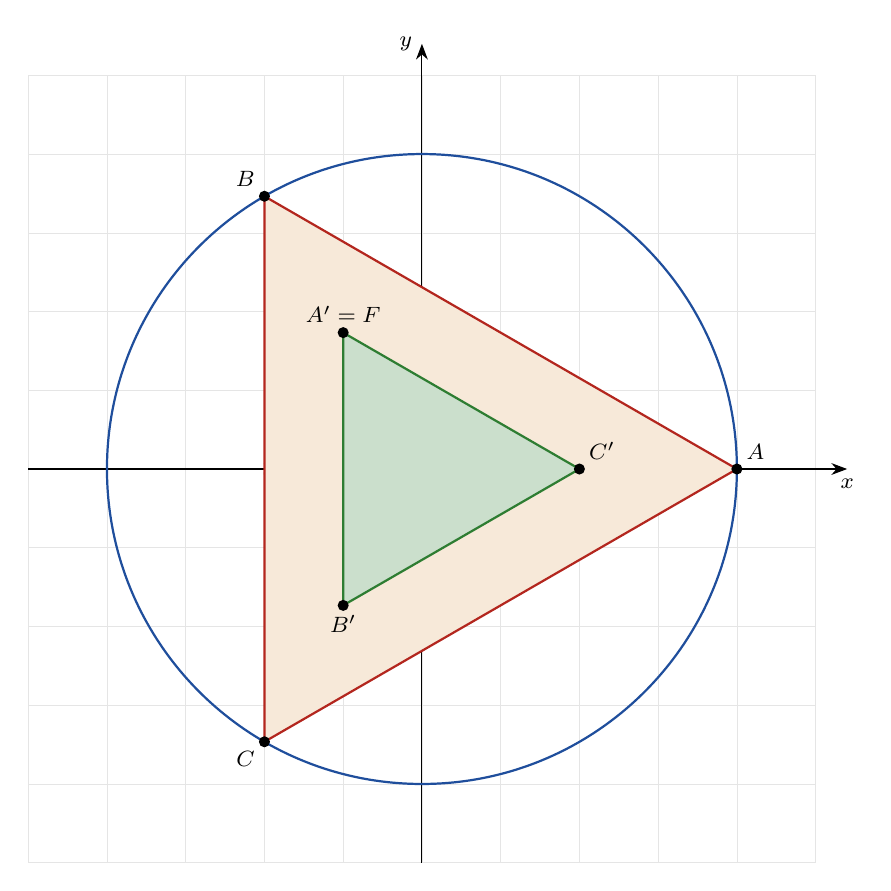
\begin{tikzpicture}[scale=2,font=\footnotesize]
\draw[gray!20,very thin,step=0.5](-2.5,-2.5) grid (2.5,2.5);
\draw[-{Stealth[length=2mm]}](-2.5,0)--(2.7,0) node[below]{$x$};
\draw[-{Stealth[length=2mm]}](0,-2.5)--(0,2.7) node[left]{$y$};
\draw[-{Stealth[length=2mm]},thick](0,0)--(1,0) node[below]{$\vec u$};
\draw[-{Stealth[length=2mm]},thick](0,0)--(0,1) node[right]{$\vec v$};
\node[below left] at (0,0){$O$};
\draw[cDef,thick](0,0) circle (2);
\draw[cRem,dashed](0,0) circle (1);
\fill[cEx!15](2,0)--(-1,1.732)--(-1,-1.732)--cycle;
\draw[cThm,thick](2,0)--(-1,1.732)--(-1,-1.732)--cycle;
\fill[cRem!25](-0.5,0.866)--(-0.5,-0.866)--(1,0)--cycle;
\draw[cRem,thick](-0.5,0.866)--(-0.5,-0.866)--(1,0)--cycle;
\fill (2,0) circle (1pt) node[above right]{$A$};
\fill (-1,1.732) circle (1pt) node[above left]{$B$};
\fill (-1,-1.732) circle (1pt) node[below left]{$C$};
\fill (-0.5,0.866) circle (1pt) node[above]{$A'=F$};
\fill (-0.5,-0.866) circle (1pt) node[below]{$B'$};
\fill (1,0) circle (1pt) node[above right]{$C'$};
\end{tikzpicture}\end{LTR}\end{center}
\end{hal}

% ===================== التمرين 13 =====================
\Needspace{12\baselineskip}
\begin{tamrin}{بكالوريا 2017 -- الدورة الاستثنائية -- الموضوع الثاني -- علوم تجريبية}
المستوي منسوب إلى المعلم المتعامد والمتجانس $(O;\vec u,\vec v)$.
نعتبر النقط $A$، $B$ و$C$ التي لاحقاتها على الترتيب: $z_A=-3-2i$، $z_B=1+i$ و$z_C=4-3i$.
\QQ{1} عين النسبة والزاوية للتشابه $S$ المباشر ذي المركز $A$ والذي يحول النقطة $B$ إلى النقطة $C$.
\QQ{2} أكتب على الشكل الأسي العدد المركب $\dfrac{z_A-z_B}{z_C-z_B}$، ثم استنتج طبيعة المثلث $ABC$.
\QQ{3} نرمز بـ $G$ إلى مركز ثقل المثلث $ABC$ وبـ $I$ إلى منتصف القطعة $[AC]$.
عين كلا من $z_G$ و$z_I$ لاحقتي النقطتين $G$ و$I$، ثم بين أن النقط $B$، $G$ و$I$ في استقامية.
\QQ{4} نعتبر النقطة $D$ نظيرة النقطة $B$ بالنسبة إلى $I$. حدد بدقة طبيعة الرباعي $ABCD$.
\QQ{5} نعتبر $(\Gamma)$ مجموعة النقط $M$ من المستوي التي تحقق: $\left\|\overrightarrow{MA}+\overrightarrow{MC}\right\|=5\sqrt2$.
\begin{sq}
\qa تحقق أن النقطة $C$ تنتمي إلى $(\Gamma)$.
\qb عين طبيعة المجموعة $(\Gamma)$ ثم أنشئها.
\end{sq}
\end{tamrin}

\begin{hal}
\QQ{1} العبارة المركبة لـ $S$: $z'-z_A=a(z-z_A)$، و$S(B)=C$ يعطي
\[a=\frac{z_C-z_A}{z_B-z_A}=\frac{7-i}{4+3i}=\frac{(7-i)(4-3i)}{16+9}=\frac{28-21i-4i-3}{25}=\frac{25-25i}{25}=1-i .\]
$1-i=\sqrt2\left(\frac{\sqrt2}{2}-\frac{\sqrt2}{2}i\right)=\sqrt2\,e^{-i\frac{\pi}{4}}$، إذن \bxt{نسبة $S$ هي $\sqrt2$ وزاويته $-\frac{\pi}{4}$}.

\QQ{2} $\dfrac{z_A-z_B}{z_C-z_B}=\dfrac{-4-3i}{3-4i}=\dfrac{(-4-3i)(3+4i)}{9+16}=\dfrac{-12-16i-9i+12}{25}=-i$،
إذن \bx{\frac{z_A-z_B}{z_C-z_B}=e^{-i\frac{\pi}{2}}}.

ومنه $BA=BC$ و$\left(\overrightarrow{BC},\overrightarrow{BA}\right)=-\dfrac{\pi}{2}$: \bxt{المثلث $ABC$ قائم ومتساوي الساقين في $B$}.

\QQ{3} $z_G=\dfrac{z_A+z_B+z_C}{3}=\dfrac{2-4i}{3}$ أي \bx{z_G=\frac23-\frac43i}، و$z_I=\dfrac{z_A+z_C}{2}$ أي \bx{z_I=\frac12-\frac52i}.

$z_G-z_B=\dfrac{2-4i}{3}-1-i=\dfrac{-1-7i}{3}$ و$z_I-z_B=\dfrac{1-5i}{2}-1-i=\dfrac{-1-7i}{2}$، ومنه
$\dfrac{z_G-z_B}{z_I-z_B}=\dfrac23\in\mathbb{R}$، أي $\overrightarrow{BG}=\dfrac23\overrightarrow{BI}$: \bxt{النقط $B$، $G$ و$I$ في استقامية}.

\QQ{4} $I$ منتصف $[BD]$: $z_D=2z_I-z_B=1-5i-1-i$ أي \bx{z_D=-6i}.
قطرا الرباعي $ABCD$ ($[AC]$ و$[BD]$) متناصفان في $I$ فهو متوازي أضلاع، وفيه $BA=BC$ (ضلعان متتاليان متقايسان) و$\widehat{ABC}$ قائمة،
إذن \bxt{$ABCD$ مربع}.

\QQ{5}
\pa $I$ منتصف $[AC]$ إذن $\overrightarrow{MA}+\overrightarrow{MC}=2\overrightarrow{MI}$. من أجل $M=C$: $\left\|\overrightarrow{CA}+\overrightarrow{CC}\right\|=CA=|z_A-z_C|=|-7+i|=\sqrt{50}=5\sqrt2$، إذن \bx{C\in(\Gamma)}.

\pb $\left\|2\overrightarrow{MI}\right\|=5\sqrt2$ يعني $MI=\dfrac{5\sqrt2}{2}$:
\bxt{$(\Gamma)$ دائرة مركزها $I$ ونصف قطرها $\frac{5\sqrt2}{2}$} (هي الدائرة التي قطرها $[AC]$، وتشمل $B$ و$D$ أيضا).

\begin{center}\begin{LTR}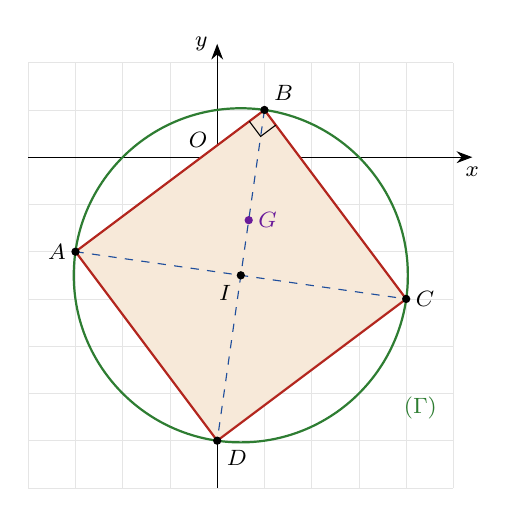
\begin{tikzpicture}[scale=0.6,font=\footnotesize]
\draw[gray!20,very thin](-4,-7) grid (5,2);
\draw[-{Stealth[length=2mm]}](-4,0)--(5.4,0) node[below]{$x$};
\draw[-{Stealth[length=2mm]}](0,-7)--(0,2.4) node[left]{$y$};
\node[above left] at (0,0){$O$};
\draw[cRem,thick](0.5,-2.5) circle (3.536);
\node[cRem] at (4.3,-5.3){$(\Gamma)$};
\fill[cEx!15](-3,-2)--(1,1)--(4,-3)--(0,-6)--cycle;
\draw[cThm,thick](-3,-2)--(1,1)--(4,-3)--(0,-6)--cycle;
\draw[cDef,dashed](-3,-2)--(4,-3) (1,1)--(0,-6);
\draw (1,1)++(-143.13:0.4)--++(-53.13:0.4)--++(36.87:0.4);
\fill (-3,-2) circle (2.5pt) node[left]{$A$};
\fill (1,1) circle (2.5pt) node[above right]{$B$};
\fill (4,-3) circle (2.5pt) node[right]{$C$};
\fill (0,-6) circle (2.5pt) node[below right]{$D$};
\fill (0.5,-2.5) circle (2.5pt) node[below left]{$I$};
\fill[cMeth] (0.667,-1.333) circle (2.5pt) node[right]{$G$};
\end{tikzpicture}\end{LTR}\end{center}
\end{hal}

% ===================== التمرين 14 =====================
\Needspace{12\baselineskip}
\begin{tamrin}{بكالوريا 2017 -- الموضوع الأول -- علوم تجريبية}
\textbf{I)} حل في المجموعة $\mathbb{C}$ المعادلة: $(z+2)\left(z^2-4z+8\right)=0$.

\textbf{II)} المستوي المركب منسوب إلى المعلم المتعامد والمتجانس $(O;\vec u,\vec v)$.
نعتبر النقط $A$، $B$ و$C$ التي لاحقاتها: $z_A=2-2i$، $z_B=\overline{z_A}$ و$z_C=-2$.
\QQ{1} أكتب كلا من العددين $z_A$ و$z_B$ على الشكل الأسي.
\QQ{2} عين $z_D$ لاحقة النقطة $D$ حتى تكون النقطة $B$ مركز ثقل المثلث $ACD$.
\QQ{3} $(\Gamma)$ مجموعة النقط $M$ من المستوي ذات اللاحقة $z$ ($M$ تختلف عن $A$ و$B$) بحيث: $\arg\left(\dfrac{z_B-z}{z_A-z}\right)=\dfrac{\pi}{2}$.
تحقق أن مبدأ المعلم $O$ هو نقطة من $(\Gamma)$ ثم عين طبيعة المجموعة $(\Gamma)$ وأنشئها.
\QQ{4} ليكن $h$ التحاكي الذي مركزه النقطة $C$ ونسبته $2$، و$(\Gamma')$ صورة $(\Gamma)$ بالتحاكي $h$.
عين طبيعة المجموعة $(\Gamma')$ مع تحديد عناصرها المميزة.
\end{tamrin}

\begin{hal}
\textbf{I)} $z=-2$، أو $z^2-4z+8=0$: $\Delta=16-32=-16=(4i)^2$ ومنه $z=\dfrac{4\pm4i}{2}=2\pm2i$.
\bx{S=\{-2\,;\,2-2i\,;\,2+2i\}}.

\textbf{II)}
\QQ{1} $|z_A|=\sqrt{4+4}=2\sqrt2$، $\cos\theta=\frac{\sqrt2}{2}$ و$\sin\theta=-\frac{\sqrt2}{2}$ إذن $\theta=-\frac{\pi}{4}$:
\bx{z_A=2\sqrt2\,e^{-i\frac{\pi}{4}}} و\bx{z_B=\overline{z_A}=2\sqrt2\,e^{i\frac{\pi}{4}}}.

\QQ{2} $B$ مركز ثقل $ACD$ يعني $z_B=\dfrac{z_A+z_C+z_D}{3}$، ومنه $z_D=3z_B-z_A-z_C=6+6i-2+2i+2$:
\bx{z_D=6+8i}.

\QQ{3} من أجل $z=0$: $\dfrac{z_B-0}{z_A-0}=\dfrac{2+2i}{2-2i}=\dfrac{(2+2i)^2}{8}=\dfrac{8i}{8}=i=e^{i\frac{\pi}{2}}$، إذن $\arg=\frac{\pi}{2}$ و\bx{O\in(\Gamma)}.

$\arg\left(\dfrac{z_B-z}{z_A-z}\right)=\dfrac{\pi}{2}$ يعني $\left(\overrightarrow{MA},\overrightarrow{MB}\right)=\dfrac{\pi}{2}$: الزاوية $\widehat{AMB}$ قائمة، إذن $M$ تنتمي إلى الدائرة التي قطرها $[AB]$ (مركزها $\Omega$ منتصف $[AB]$ ذات اللاحقة $2$ ونصف قطرها $\frac{AB}{2}=2$)، مع الاحتفاظ فقط بالنقط التي تكون فيها الزاوية الموجهة $+\frac{\pi}{2}$ (لا $-\frac{\pi}{2}$).

تحليليا: بوضع $z=x+iy$: $(z_B-z)\overline{(z_A-z)}=\left(x^2-4x+y^2\right)+i(8-4x)$، فالشرط يكافئ: الجزء الحقيقي معدوم والجزء التخيلي موجب تماما، أي
$(x-2)^2+y^2=4$ و$x<2$.

إذن \bxt{$(\Gamma)$ نصف الدائرة التي مركزها $\Omega(2)$ ونصف قطرها $2$}، الواقع في الجهة $x<2$ (الذي يشمل $O$)، محروما من $A$ و$B$.

\QQ{4} العبارة المركبة لـ $h$: $z'-z_C=2(z-z_C)$ أي $z'=2z+2$.
التحاكي يحول نصف دائرة مركزها $\Omega$ ونصف قطرها $r$ إلى نصف دائرة مركزها $h(\Omega)$ ونصف قطرها $2r$:
$z_{\Omega'}=2\times2+2=6$، $r'=2\times2=4$، وطرفاها $h(A)$ و$h(B)$: $z_{A'}=2(2-2i)+2=6-4i$، $z_{B'}=6+4i$، وتشمل $h(O)$ ذات اللاحقة $2$.

إذن \bxt{$(\Gamma')$ نصف الدائرة التي مركزها $\Omega'(6)$ ونصف قطرها $4$}، الواقع في الجهة $x<6$، محروما من $A'(6-4i)$ و$B'(6+4i)$.

\begin{center}\begin{LTR}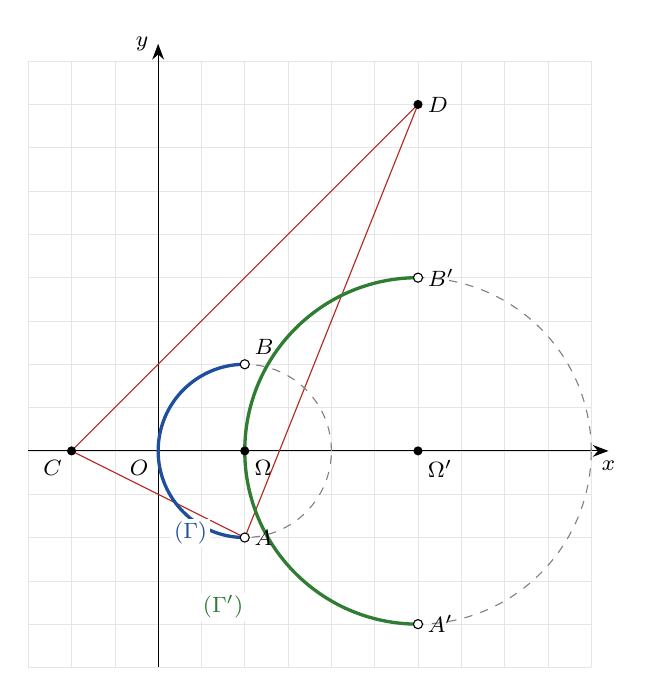
\begin{tikzpicture}[scale=0.55,font=\footnotesize]
\draw[gray!20,very thin](-3,-5) grid (10,9);
\draw[-{Stealth[length=2mm]}](-3,0)--(10.4,0) node[below]{$x$};
\draw[-{Stealth[length=2mm]}](0,-5)--(0,9.4) node[left]{$y$};
\node[below left] at (0,0){$O$};
\draw[cThm,thin](2,-2)--(-2,0)--(6,8)--cycle;
\draw[gray,dashed](2,0) circle (2);
\draw[cDef,very thick](2,2) arc (90:270:2);
\node[cDef,fill=white,inner sep=1pt] at (0.75,-1.9){$(\Gamma)$};
\draw[gray,dashed](6,0) circle (4);
\draw[cRem,very thick](6,4) arc (90:270:4);
\node[cRem,fill=white,inner sep=1pt] at (1.5,-3.6){$(\Gamma')$};
\foreach \p in {(2,2),(2,-2),(6,4),(6,-4)} \draw[fill=white] \p circle (3pt);
\node[right] at (2,-2){$A$};
\node[above right] at (2,2){$B$};
\fill (-2,0) circle (3pt) node[below left]{$C$};
\fill (6,8) circle (3pt) node[right]{$D$};
\fill (2,0) circle (3pt) node[below right]{$\Omega$};
\fill (6,0) circle (3pt) node[below right]{$\Omega'$};
\node[right] at (6,4){$B'$};
\node[right] at (6,-4){$A'$};
\end{tikzpicture}\end{LTR}\end{center}
\end{hal}

% ===================== التمرين 15 =====================
\Needspace{12\baselineskip}
\begin{tamrin}{بكالوريا 2017 -- الموضوع الثاني -- علوم تجريبية}
المستوي المركب منسوب إلى المعلم المتعامد والمتجانس $(O;\vec u,\vec v)$.
أجب بصحيح أو خطأ مع التعليل في كل حالة مما يلي:
\QQ{1} مجموعة حلول المعادلة $\left(\dfrac{z+1-i}{z-i}\right)^2=1$ في المجموعة $\mathbb{C}$ هي: $S=\left\{-\dfrac12+i\right\}$.
\QQ{2} من أجل كل عدد مركب $z$، $(z+2)\left(\overline{z}+2\right)=|z+2|^2$.
\QQ{3} من أجل كل عدد طبيعي $n$، $\left(\dfrac12+i\dfrac{\sqrt3}{2}\right)^{3n}=1$.
\QQ{4} $S$ التشابه المباشر الذي مركزه $\Omega$ ذات اللاحقة $1$ ونسبته $3$ وزاويته $\dfrac{\pi}{2}$.
صورة الدائرة $(C)$ ذات المركز $\omega(0;1)$ ونصف القطر $3$ بالتشابه $S$ هي الدائرة $(C')$ ذات المركز $\omega'(-2;-3)$ ونصف القطر $9$.
\QQ{5} من أجل كل عدد حقيقي $\alpha$: إذا كان $z=(\sin\alpha+i\cos\alpha)\times(\cos\alpha-i\sin\alpha)$ فإن: $\arg(z)=\dfrac{\pi}{2}-2\alpha+2k\pi$ حيث $k$ عدد صحيح.
\end{tamrin}

\begin{hal}
\QQ{1} \bxt{صحيح}. من أجل $z\neq i$ نضع $w=\dfrac{z+1-i}{z-i}$: $w^2=1$ يعني $w=1$ أو $w=-1$.
\begin{itemize}
\item $w=1$: $z+1-i=z-i$ أي $1=0$: مستحيل.
\item $w=-1$: $z+1-i=-z+i$ أي $2z=-1+2i$ أي $z=-\frac12+i$ (وهو يختلف عن $i$).
\end{itemize}
إذن $S=\left\{-\frac12+i\right\}$.

\QQ{2} \bxt{صحيح}. $\overline{z+2}=\overline{z}+2$، و$w\,\overline{w}=|w|^2$ من أجل كل $w$، إذن $(z+2)\left(\overline{z}+2\right)=(z+2)\overline{(z+2)}=|z+2|^2$.

\QQ{3} \bxt{خطأ}. $\dfrac12+i\dfrac{\sqrt3}{2}=e^{i\frac{\pi}{3}}$، ومنه $\left(e^{i\frac{\pi}{3}}\right)^{3n}=e^{in\pi}=(-1)^n$.
مثال مضاد: من أجل $n=1$ نجد $-1\neq1$.

\QQ{4} \bxt{صحيح}. العبارة المركبة لـ $S$: $z'-1=3e^{i\frac{\pi}{2}}(z-1)$ أي $z'=3i(z-1)+1$.
مركز $(C)$ هو $\omega$ ذات اللاحقة $i$، وصورته: $3i(i-1)+1=-3-3i+1=-2-3i$ أي $\omega'(-2;-3)$ \ok.
التشابه ذو النسبة $3$ يحول دائرة نصف قطرها $3$ إلى دائرة نصف قطرها $3\times3=9$ \ok.

\QQ{5} \bxt{صحيح}. $\sin\alpha+i\cos\alpha=\cos\left(\frac{\pi}{2}-\alpha\right)+i\sin\left(\frac{\pi}{2}-\alpha\right)=e^{i\left(\frac{\pi}{2}-\alpha\right)}$ و$\cos\alpha-i\sin\alpha=e^{-i\alpha}$،
إذن $z=e^{i\left(\frac{\pi}{2}-2\alpha\right)}$ (طويلته $1\neq0$) و$\arg(z)=\dfrac{\pi}{2}-2\alpha+2k\pi$.
\end{hal}
% ===================== التمرين 16 =====================
\Needspace{12\baselineskip}
\begin{tamrin}{بكالوريا 2016 -- الدورة الثانية -- الموضوع الأول -- علوم تجريبية}
\QQ{1} نضع من أجل كل عدد مركب $z$: $P(z)=z^3-24\sqrt3$.
\begin{sq}
\qa تحقق أن: $P\left(2\sqrt3\right)=0$.
\qb جد العددين الحقيقيين $a$ و$b$ بحيث من أجل كل عدد مركب $z$: $P(z)=\left(z-2\sqrt3\right)\left(z^2+az+b\right)$.
\qc حل في مجموعة الأعداد المركبة $\mathbb{C}$ المعادلة $P(z)=0$.
\end{sq}
\QQ{2} المستوي منسوب إلى المعلم المتعامد والمتجانس $(O;\vec u,\vec v)$. $A$، $B$ و$C$ نقط من المستوي لواحقها على الترتيب: $z_A=-\sqrt3+3i$، $z_B=-\sqrt3-3i$ و$z_C=2\sqrt3$.
\begin{sq}
\qa أكتب على الشكل الجبري العدد المركب $\dfrac{z_C-z_A}{z_B-z_A}$.
\qb بين أنه يوجد دوران $R$ مركزه $A$ ويحول النقطة $B$ إلى النقطة $C$، يطلب تعيين زاويته.
\qc استنتج طبيعة المثلث $ABC$.
\qd عين $z_D$ لاحقة النقطة $D$ صورة النقطة $C$ بالانسحاب الذي شعاعه $\overrightarrow{AB}$، ثم حدد بدقة طبيعة الرباعي $ABDC$.
\end{sq}
\QQ{3} عين $(\Gamma)$ مجموعة النقط $M$ من المستوي ذات اللاحقة غير المعدومة $z$ بحيث: $\arg\left(\dfrac{z}{\overline{z}}\right)=2k\pi$ حيث $k\in\mathbb{Z}$.
\end{tamrin}

\begin{hal}
\QQ{1}
\pa $\left(2\sqrt3\right)^3=8\times3\sqrt3=24\sqrt3$، إذن $P\left(2\sqrt3\right)=24\sqrt3-24\sqrt3$ أي \bx{P\left(2\sqrt3\right)=0}.

\pb ننشر: $\left(z-2\sqrt3\right)\left(z^2+az+b\right)=z^3+\left(a-2\sqrt3\right)z^2+\left(b-2\sqrt3\,a\right)z-2\sqrt3\,b$.
بالمطابقة مع $z^3+0\cdot z^2+0\cdot z-24\sqrt3$:
\[\begin{cases}a-2\sqrt3=0\\ b-2\sqrt3\,a=0\\ -2\sqrt3\,b=-24\sqrt3\end{cases}\iff\begin{cases}a=2\sqrt3\\ b=12\end{cases}\]
إذن \bx{a=2\sqrt3} و\bx{b=12}، أي $P(z)=\left(z-2\sqrt3\right)\left(z^2+2\sqrt3\,z+12\right)$.

\pc $P(z)=0$ يعني $z=2\sqrt3$ أو $z^2+2\sqrt3\,z+12=0$.
$\Delta=12-48=-36=(6i)^2$، ومنه $z=\dfrac{-2\sqrt3\pm6i}{2}=-\sqrt3\pm3i$.
\bx{S=\left\{2\sqrt3\,;\,-\sqrt3+3i\,;\,-\sqrt3-3i\right\}}.

\QQ{2}
\pa $z_C-z_A=3\sqrt3-3i$ و$z_B-z_A=-6i$، ومنه
\[\frac{z_C-z_A}{z_B-z_A}=\frac{3\sqrt3-3i}{-6i}=\frac{\left(3\sqrt3-3i\right)i}{6}=\frac{3+3\sqrt3\,i}{6}\qquad\Longrightarrow\qquad \bx{\frac{z_C-z_A}{z_B-z_A}=\frac12+\frac{\sqrt3}{2}i}.\]

\pb $\dfrac12+\dfrac{\sqrt3}{2}i=e^{i\frac{\pi}{3}}$، إذن $z_C-z_A=e^{i\frac{\pi}{3}}(z_B-z_A)$: وهي من الشكل $z'-z_A=e^{i\theta}(z-z_A)$.
إذن \bxt{$C=R(B)$ حيث $R$ الدوران الذي مركزه $A$ وزاويته $\frac{\pi}{3}$}.

\pc $R(B)=C$ يعني $AB=AC$ و$\left(\overrightarrow{AB},\overrightarrow{AC}\right)=\frac{\pi}{3}$، إذن \bxt{المثلث $ABC$ متقايس الأضلاع} (طول ضلعه $AB=|-6i|=6$).

\pd $z_D=z_C+(z_B-z_A)=2\sqrt3-6i$ أي \bx{z_D=2\sqrt3-6i}.

$\overrightarrow{CD}=\overrightarrow{AB}$ إذن $ABDC$ متوازي أضلاع، وفيه $AB=AC$ (ضلعان متتاليان متقايسان)، والزاوية $\widehat{BAC}=\frac{\pi}{3}$ ليست قائمة.
إذن \bxt{$ABDC$ معين (وليس مربعا)}.

\QQ{3} نضع $z=re^{i\theta}$ مع $r>0$: $\overline{z}=re^{-i\theta}$ و$\dfrac{z}{\overline{z}}=e^{2i\theta}$، إذن $\arg\left(\dfrac{z}{\overline{z}}\right)=2\theta$.
$2\theta=2k\pi$ يعني $\theta=k\pi$: $z$ عدد حقيقي غير معدوم.
إذن \bxt{$(\Gamma)$ هي محور الفواصل محروما من النقطة $O$}.

\begin{center}\begin{LTR}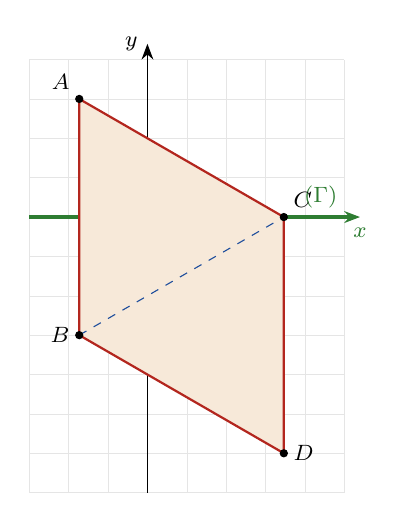
\begin{tikzpicture}[scale=0.5,font=\footnotesize]
\draw[gray!20,very thin](-3,-7) grid (5,4);
\draw[-{Stealth[length=2mm]}](0,-7)--(0,4.4) node[left]{$y$};
\draw[cRem,very thick,-{Stealth[length=2mm]}](-3,0)--(5.4,0) node[below]{$x$};
\draw[cRem,fill=white](0,0) circle (4pt);
\node[below left] at (0,0){$O$};
\node[cRem] at (4.4,0.5){$(\Gamma)$};
\fill[cEx!15](-1.732,3)--(-1.732,-3)--(3.464,-6)--(3.464,0)--cycle;
\draw[cThm,thick](-1.732,3)--(-1.732,-3)--(3.464,-6)--(3.464,0)--cycle;
\draw[cDef,dashed](-1.732,-3)--(3.464,0);
\fill (-1.732,3) circle (3pt) node[above left]{$A$};
\fill (-1.732,-3) circle (3pt) node[left]{$B$};
\fill (3.464,0) circle (3pt) node[above right]{$C$};
\fill (3.464,-6) circle (3pt) node[right]{$D$};
\end{tikzpicture}\end{LTR}\end{center}
\end{hal}

% ===================== التمرين 17 =====================
\Needspace{12\baselineskip}
\begin{tamrin}{بكالوريا 2016 -- الدورة الثانية -- الموضوع الثاني -- علوم تجريبية}
نعتبر في المجموعة $\mathbb{C}$ المعادلة ذات المجهول $z$ التالية: $2\overline{z}^{\,3}+3\overline{z}^{\,2}-3\overline{z}+5=0\ \ldots\ (E)$.
يشير الرمز $\overline{z}$ إلى مرافق العدد المركب $z$.
\QQ{1}
\begin{sq}
\qa أثبت أن المعادلة $(E)$ تكافئ المعادلة: $\left(2\overline{z}+5\right)\left(\overline{z}^{\,2}-\overline{z}+1\right)=0$.
\qb حل في المجموعة $\mathbb{C}$ المعادلة $(E)$.
\end{sq}
\QQ{2} في المستوي المركب المنسوب إلى المعلم المتعامد والمتجانس $(O;\vec u,\vec v)$ نعتبر النقط $A$، $B$، $C$ و$D$ التي لواحقها على الترتيب: $z_A=\dfrac12-i\dfrac{\sqrt3}{2}$، $z_B=\overline{z_A}$، $z_C=-1$ و$z_D=-\dfrac52$.
\begin{sq}
\qa أكتب كلا من العددين $z_A$ و$z_B$ على الشكل الأسي.
\qb أنشئ النقط $A$، $B$، $C$ و$D$.
\qc أثبت أن: $z_B-z_C=z_B\,(z_A-z_C)$.
\qd استنتج طبيعة المثلث $ABC$.
\end{sq}
\QQ{3} ليكن $S$ التشابه المباشر الذي مركزه $C$ ونسبته $2$ وزاويته $\dfrac{\pi}{3}$، ولتكن $F$ صورة $A$ بالتحويل $S$.
أنشئ النقطة $F$ ثم حدد طبيعة المثلث $AFC$.
\QQ{4} عين طبيعة المجموعة $(\gamma)$ للنقط $M$ من المستوي ذات اللاحقة $z$ حيث $z+1=kz_B$، لما $k$ يتغير في المجموعة $\mathbb{R}_+$.
\end{tamrin}

\begin{hal}
\QQ{1}
\pa ننشر الطرف الأيمن:
\[\left(2\overline{z}+5\right)\left(\overline{z}^{\,2}-\overline{z}+1\right)=2\overline{z}^{\,3}-2\overline{z}^{\,2}+2\overline{z}+5\overline{z}^{\,2}-5\overline{z}+5=2\overline{z}^{\,3}+3\overline{z}^{\,2}-3\overline{z}+5 .\]
إذن \bxt{$(E)$ تكافئ $\left(2\overline{z}+5\right)\left(\overline{z}^{\,2}-\overline{z}+1\right)=0$}.

\pb نضع $w=\overline{z}$:
\begin{itemize}
\item $2w+5=0$ يعني $w=-\frac52$، ومنه $z=\overline{w}=-\frac52$.
\item $w^2-w+1=0$: $\Delta=1-4=-3=\left(i\sqrt3\right)^2$، ومنه $w=\frac12\pm\frac{\sqrt3}{2}i$، و$z=\overline{w}=\frac12\mp\frac{\sqrt3}{2}i$.
\end{itemize}
\bx{S=\left\{-\frac52\,;\,\frac12-\frac{\sqrt3}{2}i\,;\,\frac12+\frac{\sqrt3}{2}i\right\}}.

\QQ{2}
\pa $|z_A|=\sqrt{\frac14+\frac34}=1$، $\cos\theta=\frac12$ و$\sin\theta=-\frac{\sqrt3}{2}$ إذن $\theta=-\frac{\pi}{3}$:
\bx{z_A=e^{-i\frac{\pi}{3}}} و\bx{z_B=\overline{z_A}=e^{i\frac{\pi}{3}}}.

\pb الإنشاء في الشكل أدناه ($A$ و$B$ على الدائرة المثلثية، $C$ و$D$ على محور الفواصل).

\pc $z_B-z_C=\frac12+\frac{\sqrt3}{2}i+1=\frac32+\frac{\sqrt3}{2}i$.
و$z_A-z_C=\frac32-\frac{\sqrt3}{2}i$، ومنه
\[z_B(z_A-z_C)=\left(\frac12+\frac{\sqrt3}{2}i\right)\left(\frac32-\frac{\sqrt3}{2}i\right)=\frac34-\frac{\sqrt3}{4}i+\frac{3\sqrt3}{4}i+\frac34=\frac32+\frac{\sqrt3}{2}i .\]
إذن \bx{z_B-z_C=z_B\,(z_A-z_C)}.

\pd من (جـ): $\dfrac{z_B-z_C}{z_A-z_C}=z_B=e^{i\frac{\pi}{3}}$، إذن $CB=CA$ و$\left(\overrightarrow{CA},\overrightarrow{CB}\right)=\frac{\pi}{3}$:
\bxt{المثلث $ABC$ متقايس الأضلاع}.

\QQ{3} العبارة المركبة لـ $S$: $z'-z_C=2e^{i\frac{\pi}{3}}(z-z_C)$ أي $z'=\left(1+i\sqrt3\right)(z+1)-1$.
\[z_F=\left(1+i\sqrt3\right)\left(\frac32-\frac{\sqrt3}{2}i\right)-1=\left(\frac32+\frac32\right)+i\left(\frac{3\sqrt3}{2}-\frac{\sqrt3}{2}\right)-1\]
أي \bx{z_F=2+i\sqrt3}.
طبيعة $AFC$: $\dfrac{z_F-z_A}{z_C-z_A}=\dfrac{\frac32+\frac{3\sqrt3}{2}i}{-\frac32+\frac{\sqrt3}{2}i}=-i\sqrt3=\sqrt3\,e^{-i\frac{\pi}{2}}$:
عدد تخيلي صرف، إذن $(AF)\perp(AC)$ و$AF=\sqrt3\,AC$.
\bxt{المثلث $AFC$ قائم في $A$} (وفيه $CF=2CA$ و$\widehat{ACF}=\frac{\pi}{3}$).

\QQ{4} $z+1=kz_B$ تعني $z-z_C=k\,e^{i\frac{\pi}{3}}$ أي $\overrightarrow{CM}=k\,\vec w$ حيث $\vec w$ الشعاع ذو اللاحقة $z_B$ (أي $\overrightarrow{OB}$)، مع $k\geq0$.
من أجل $k=0$ نجد $M=C$. إذن
\bxt{$(\gamma)$ نصف المستقيم الذي مبدؤه $C$ وشعاع توجيهه $\overrightarrow{OB}$}
(يصنع الزاوية $\frac{\pi}{3}$ مع $\vec u$، ويشمل النقطة ذات اللاحقة $i\sqrt3$ الموافقة لـ $k=2$).

\begin{center}\begin{LTR}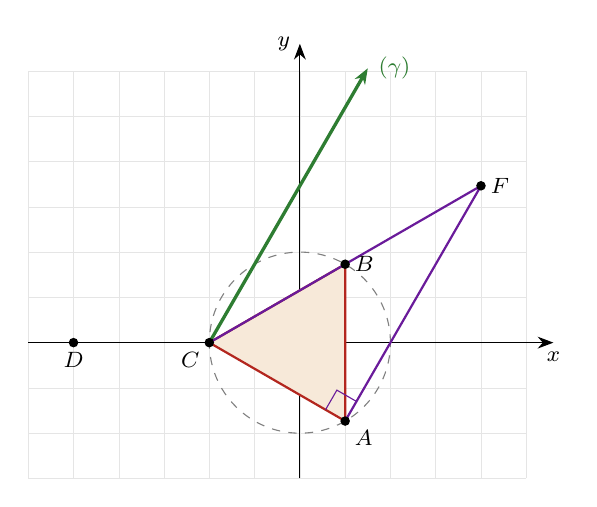
\begin{tikzpicture}[scale=1.15,font=\footnotesize]
\draw[gray!20,very thin,step=0.5](-3,-1.5) grid (2.5,3);
\draw[-{Stealth[length=2mm]}](-3,0)--(2.8,0) node[below]{$x$};
\draw[-{Stealth[length=2mm]}](0,-1.5)--(0,3.3) node[left]{$y$};
\node[below right] at (0,0){$O$};
\draw[gray,dashed](0,0) circle (1);
\draw[cRem,very thick,-{Stealth[length=2mm]}](-1,0)--(0.75,3.03) node[right]{$(\gamma)$};
\draw[cDef,-{Stealth[length=2mm]}](0,0)--(0.5,0.866);
\fill[cEx!15](0.5,-0.866)--(0.5,0.866)--(-1,0)--cycle;
\draw[cThm,thick](0.5,-0.866)--(0.5,0.866)--(-1,0)--cycle;
\draw[cMeth,thick](0.5,-0.866)--(2,1.732)--(-1,0);
\draw[cMeth] (0.5,-0.866)++(60.0:0.25)--++(150:0.25)--++(240:0.25);
\fill (0.5,-0.866) circle (1.5pt) node[below right]{$A$};
\fill (0.5,0.866) circle (1.5pt) node[right]{$B$};
\fill (-1,0) circle (1.5pt) node[below left]{$C$};
\fill (-2.5,0) circle (1.5pt) node[below]{$D$};
\fill (2,1.732) circle (1.5pt) node[right]{$F$};
\end{tikzpicture}\end{LTR}\end{center}
\end{hal}

% ===================== التمرين 18 =====================
\Needspace{12\baselineskip}
\begin{tamrin}{بكالوريا 2016 -- الدورة الأولى -- الموضوع الأول -- علوم تجريبية}
المستوي المركب منسوب إلى المعلم المتعامد والمتجانس $(O;\vec u,\vec v)$. من أجل كل نقطة $M$ من المستوي لاحقتها العدد المركب $z$ ($z\neq1$) نرفق النقطة $M'$ لاحقتها العدد المركب $z'$ حيث: $z'=\dfrac{z-2}{z-1}$.
\QQ{1} حل في $\mathbb{C}$ المعادلة ذات المجهول $z$: $z'=z$.
\QQ{2} النقطتان $A$ و$B$ لاحقتاهما $z_1$ و$z_2$ على الترتيب حيث: $z_1=1-i$، $z_2=\overline{z_1}$.
\begin{sq}
\qa أكتب $\dfrac{z_2}{z_1}$ على الشكل الأسي.
\qb بين أن النقطة $B$ صورة النقطة $A$ بالدوران $R$ الذي مركزه المبدأ $O$، يطلب تعيين زاوية له.
\end{sq}
\QQ{3} نضع: $z'\neq z$. نعتبر النقطتين $C$ و$D$ لاحقتيهما $2$ و$1$ على الترتيب.
عين $(\Gamma)$ مجموعة النقط $M$ حيث $M'$ تنتمي إلى محور التراتيب ثم أنشئه.
\QQ{4} $h$ التحاكي الذي مركزه المبدأ $O$ ونسبته $2$.
\begin{sq}
\qa عين طبيعة التحويل النقطي $S=h\circ R$ وعناصره المميزة.
\qb أكتب العبارة المركبة للتحويل $S$.
\qc عين ثم أنشئ المجموعة $(\Gamma')$ صورة $(\Gamma)$ بالتحويل $S$.
\end{sq}
\end{tamrin}

\begin{hal}
\QQ{1} من أجل $z\neq1$: $\dfrac{z-2}{z-1}=z$ يعني $z-2=z^2-z$ أي $z^2-2z+2=0$.
$\Delta=4-8=-4=(2i)^2$ ومنه $z=1-i$ أو $z=1+i$ (وكلاهما يختلف عن $1$).
\bx{S=\{1-i\,;\,1+i\}}.

\QQ{2}
\pa $\dfrac{z_2}{z_1}=\dfrac{1+i}{1-i}=\dfrac{(1+i)^2}{(1-i)(1+i)}=\dfrac{2i}{2}=i$، إذن \bx{\frac{z_2}{z_1}=e^{i\frac{\pi}{2}}}.

\pb $z_2=e^{i\frac{\pi}{2}}z_1$ من الشكل $z'=e^{i\theta}z$: إذن \bxt{$B=R(A)$ حيث $R$ الدوران الذي مركزه $O$ وزاويته $\frac{\pi}{2}$}.

\QQ{3} $M'$ تنتمي إلى محور التراتيب يعني $z'$ تخيلي صرف أو معدوم، أي $\operatorname{Re}(z')=0$.

\textbf{طريقة هندسية:} $z'=\dfrac{z_C-z}{z_D-z}$. إذا كان $z'=0$ فإن $M=C$. وإذا كان $z'\neq0$ فإن $z'$ تخيلي صرف يعني $\left(\overrightarrow{MD},\overrightarrow{MC}\right)=\pm\frac{\pi}{2}$ أي $(MC)\perp(MD)$: $M$ على الدائرة التي قطرها $[CD]$.

\textbf{طريقة تحليلية:} نضع $z=x+iy$ ($z\neq1$):
\[z'=\frac{(z-2)\left(\overline{z}-1\right)}{|z-1|^2}\quad,\quad \operatorname{Re}\left[(z-2)\left(\overline{z}-1\right)\right]=(x-2)(x-1)+y^2=x^2-3x+2+y^2 .\]
$\operatorname{Re}(z')=0$ يعني $x^2-3x+2+y^2=0$ أي $\left(x-\frac32\right)^2+y^2=\frac14$ مع $(x;y)\neq(1;0)$.

إذن \bxt{$(\Gamma)$ الدائرة التي مركزها $\Omega\left(\frac32;0\right)$ ونصف قطرها $\frac12$ محرومة من $D$}، وهي الدائرة التي قطرها $[CD]$.
(الشرط $z'\neq z$ يستبعد النقطتين ذواتي اللاحقتين $1\pm i$ فقط، وهما لا تنتميان إلى هذه الدائرة، فلا يغير النتيجة.)

\QQ{4}
\pa مركب دوران وتحاك لهما نفس المركز $O$ هو تشابه مباشر:
\bxt{$S$ تشابه مباشر مركزه $O$، نسبته $2$ وزاويته $\frac{\pi}{2}$}.

\pb $R:\ z'=iz$ و$h:\ z'=2z$، إذن $S=h\circ R:\ z'=2(iz)$ أي \bx{z'=2iz}.

\pc التشابه يحول دائرة إلى دائرة: المركز $S(\Omega)$ لاحقته $2i\times\frac32=3i$، ونصف القطر $2\times\frac12=1$، والنقطة المستبعدة $S(D)$ لاحقتها $2i$.
\bxt{$(\Gamma')$ الدائرة التي مركزها $\Omega'(0;3)$ ونصف قطرها $1$ محرومة من النقطة $D'(0;2)$}.

\begin{center}\begin{LTR}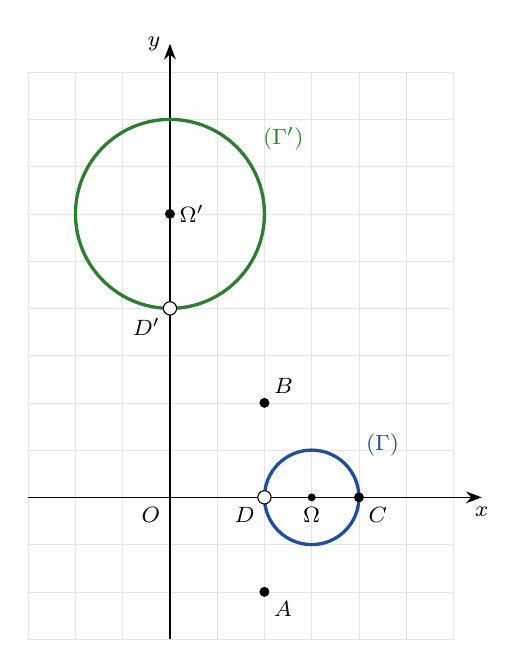
\begin{tikzpicture}[scale=1.2,font=\footnotesize]
\draw[gray!20,very thin,step=0.5](-1.5,-1.5) grid (3,4.5);
\draw[-{Stealth[length=2mm]}](-1.5,0)--(3.3,0) node[below]{$x$};
\draw[-{Stealth[length=2mm]}](0,-1.5)--(0,4.8) node[left]{$y$};
\node[below left] at (0,0){$O$};
\draw[cDef,very thick](1.5,0) circle (0.5);
\node[cDef] at (2.25,0.55){$(\Gamma)$};
\draw[cRem,very thick](0,3) circle (1);
\node[cRem] at (1.2,3.8){$(\Gamma')$};
\draw[fill=white](1,0) circle (2pt) node[below left]{$D$};
\draw[fill=white](0,2) circle (2pt) node[below left]{$D'$};
\fill (2,0) circle (1.5pt) node[below right]{$C$};
\fill (1.5,0) circle (1.2pt) node[below]{$\Omega$};
\fill (0,3) circle (1.5pt) node[right]{$\Omega'$};
\fill (1,-1) circle (1.5pt) node[below right]{$A$};
\fill (1,1) circle (1.5pt) node[above right]{$B$};
\end{tikzpicture}\end{LTR}\end{center}
\end{hal}

% ===================== التمرين 19 =====================
\Needspace{12\baselineskip}
\begin{tamrin}{بكالوريا 2016 -- الدورة الأولى -- الموضوع الثاني -- علوم تجريبية}
\QQ{1} حل في مجموعة الأعداد المركبة $\mathbb{C}$ المعادلة ذات المجهول $z$ التالية: $\left(z-\dfrac{\sqrt3}{2}-\dfrac12i\right)\left(z^2+\sqrt3\,z+1\right)=0$.
\QQ{2} المستوي المركب منسوب إلى المعلم المتعامد والمتجانس $(O;\vec u,\vec v)$.
$A$، $B$ و$C$ ثلاث نقط من المستوي لواحقها على الترتيب: $z_A=\dfrac{\sqrt3}{2}+\dfrac12i$، $z_B=-\dfrac{\sqrt3}{2}+\dfrac12i$ و$z_C=\overline{z_B}$.
\begin{sq}
\qa أكتب $z_A$، $z_B$ و$z_C$ على الشكل الأسي.
\qb بين أنه يوجد تشابه مباشر $S$ مركزه $B$ ويحول النقطة $A$ إلى النقطة $C$، يطلب تعيين عناصره المميزة.
\end{sq}
\QQ{3}
\begin{sq}
\qa عين لاحقة النقطة $D$ حتى يكون الرباعي $ABCD$ متوازي أضلاع، ثم حدد بدقة طبيعته.
\qb عين $(E)$ مجموعة النقط $M$ ذات اللاحقة $z$ والتي تحقق: $|z-z_A|=\left|\overline{z}-z_B\right|$.
\qc عين $(\Gamma)$ مجموعة النقط $M$ ذات اللاحقة $z$ والتي تحقق: $z=z_B+\sqrt3\,e^{i\theta}$ عندما $\theta$ يتغير على $\mathbb{R}$، ثم تحقق أن $A\in(\Gamma)$.
\end{sq}
\end{tamrin}

\begin{hal}
\QQ{1} $z=\dfrac{\sqrt3}{2}+\dfrac12i$، أو $z^2+\sqrt3\,z+1=0$: $\Delta=3-4=-1=i^2$ ومنه $z=\dfrac{-\sqrt3\pm i}{2}$.
\bx{S=\left\{\frac{\sqrt3}{2}+\frac12i\,;\,-\frac{\sqrt3}{2}+\frac12i\,;\,-\frac{\sqrt3}{2}-\frac12i\right\}}.

\QQ{2}
\pa $|z_A|=|z_B|=|z_C|=\sqrt{\frac34+\frac14}=1$.
$z_A$: $\cos\theta=\frac{\sqrt3}{2}$، $\sin\theta=\frac12$ إذن \bx{z_A=e^{i\frac{\pi}{6}}}.
$z_B$: $\cos\theta=-\frac{\sqrt3}{2}$، $\sin\theta=\frac12$ إذن \bx{z_B=e^{i\frac{5\pi}{6}}}، و\bx{z_C=\overline{z_B}=e^{-i\frac{5\pi}{6}}}.

\pb نبحث عن $S$ من الشكل $z'-z_B=a(z-z_B)$ مع $S(A)=C$:
\[a=\frac{z_C-z_B}{z_A-z_B}=\frac{-i}{\sqrt3}=\frac{\sqrt3}{3}\,e^{-i\frac{\pi}{2}} .\]
$a\neq0$ و$a\neq1$، إذن يوجد تشابه مباشر $S$ عبارته $z'=-\frac{\sqrt3}{3}i\left(z-z_B\right)+z_B$:
\bxt{مركزه $B$، نسبته $\frac{\sqrt3}{3}$ وزاويته $-\frac{\pi}{2}$}.

\QQ{3}
\pa $ABCD$ متوازي أضلاع يعني $\overrightarrow{AD}=\overrightarrow{BC}$ أي $z_D=z_A+z_C-z_B=\frac{\sqrt3}{2}+\frac12i-i$:
\bx{z_D=\frac{\sqrt3}{2}-\frac12i}.

طبيعته: $AB=|z_B-z_A|=\left|-\sqrt3\right|=\sqrt3$، $BC=|z_C-z_B|=|-i|=1$، و$\dfrac{z_A-z_B}{z_C-z_B}=\dfrac{\sqrt3}{-i}=i\sqrt3$ تخيلي صرف إذن $(BA)\perp(BC)$.
متوازي أضلاع له زاوية قائمة وضلعان متتاليان غير متقايسين: \bxt{$ABCD$ مستطيل (وليس مربعا)}.

\pb $\left|\overline{z}-z_B\right|=\left|\overline{z-\overline{z_B}}\right|=|z-z_C|$، إذن الشرط يكافئ $|z-z_A|=|z-z_C|$ أي $MA=MC$:
\bxt{$(E)$ محور القطعة $[AC]$}.
وبما أن $z_C=-z_A$ فإن $O$ منتصف $[AC]$، و$(E)$ هو المستقيم المار بـ $O$ والعمودي على $(OA)$، معادلته $y=-\sqrt3\,x$.

\pc $z-z_B=\sqrt3\,e^{i\theta}$ يعني $|z-z_B|=\sqrt3$ أي $BM=\sqrt3$، و$\theta$ يمسح $\mathbb{R}$ فتمسح $M$ كل الدائرة:
\bxt{$(\Gamma)$ الدائرة التي مركزها $B$ ونصف قطرها $\sqrt3$}.
$|z_A-z_B|=\sqrt3$ إذن \bx{A\in(\Gamma)} (توافق $\theta=0$: $z_B+\sqrt3=\frac{\sqrt3}{2}+\frac12i=z_A$).

\begin{center}\begin{LTR}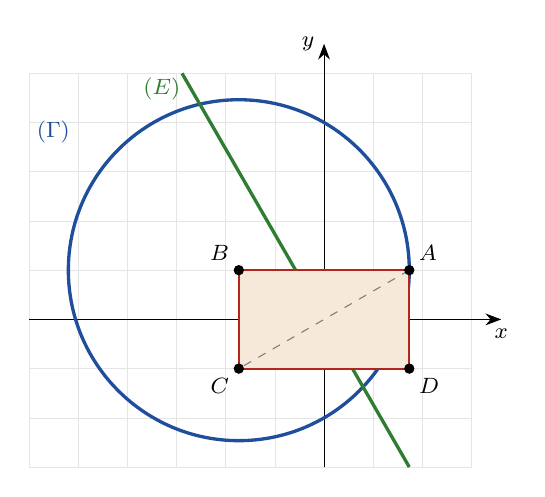
\begin{tikzpicture}[scale=1.25,font=\footnotesize]
\draw[gray!20,very thin,step=0.5](-3,-1.5) grid (1.5,2.5);
\draw[-{Stealth[length=2mm]}](-3,0)--(1.8,0) node[below]{$x$};
\draw[-{Stealth[length=2mm]}](0,-1.5)--(0,2.8) node[left]{$y$};
\node[below right] at (0,0){$O$};
\draw[cDef,very thick](-0.866,0.5) circle (1.732);
\node[cDef] at (-2.75,1.9){$(\Gamma)$};
\draw[cRem,very thick](-1.443,2.5)--(0.866,-1.5) node[pos=0.04,left]{$(E)$};
\fill[cEx!15](0.866,0.5)--(-0.866,0.5)--(-0.866,-0.5)--(0.866,-0.5)--cycle;
\draw[cThm,thick](0.866,0.5)--(-0.866,0.5)--(-0.866,-0.5)--(0.866,-0.5)--cycle;
\draw[gray,dashed](0.866,0.5)--(-0.866,-0.5);
\fill (0.866,0.5) circle (1.5pt) node[above right]{$A$};
\fill (-0.866,0.5) circle (1.5pt) node[above left]{$B$};
\fill (-0.866,-0.5) circle (1.5pt) node[below left]{$C$};
\fill (0.866,-0.5) circle (1.5pt) node[below right]{$D$};
\end{tikzpicture}\end{LTR}\end{center}
\end{hal}
% ====================== التمرين: 2015 م1 ======================
\begin{tamrin}{بكالوريا 2015 -- الموضوع الأول -- علوم تجريبية}
\textbf{I)} عيّن العددين المركّبين $\alpha$ و$\beta$ حيث:
\[\begin{cases}2\alpha-\beta=-3\\[2pt] 2\overline{\alpha}+\overline{\beta}=-3-2i\sqrt3\end{cases}\]
مع $\overline{\alpha}$ مرافق $\alpha$ و$\overline{\beta}$ مرافق $\beta$.

\textbf{II)} المستوي منسوب إلى المعلم المتعامد والمتجانس $(O;\vec u,\vec v)$. $A$، $B$ و$C$ النقط التي لواحقها على الترتيب:
\[z_A=-\frac32+i\frac{\sqrt3}{2},\qquad z_B=\overline{z_A},\qquad z_A=z_C\,e^{i\frac{\pi}{3}}.\]
\textbf{1)}
\begin{sq}
\qa اكتب $z_A$ و$z_C$ على الشكل الأسّي، ثم عيّن قيم العدد الطبيعي $n$ بحيث يكون $\left(\dfrac{z_A}{z_C}\right)^{n}$ حقيقيًا سالبًا.
\qb تحقّق أنّ العدد المركّب $2\left(\dfrac{z_A}{\sqrt3}\right)^{2015}+\left(\dfrac{z_B}{\sqrt3}\right)^{1962}-\left(\dfrac{z_C}{\sqrt3}\right)^{1435}$ حقيقي.
\end{sq}
\textbf{2)} $D$ النقطة ذات اللاحقة $z_D=1+i$.
\begin{sq}
\qa حدّد النسبة والزاوية للتشابه $S$ الذي مركزه $O$ ويحوّل $D$ إلى $A$.
\qb اكتب $\dfrac{z_A}{z_D}$ على الشكل الجبري، ثم استنتج القيمة المضبوطة لكلّ من $\cos\left(\dfrac{7\pi}{12}\right)$ و$\sin\left(\dfrac{7\pi}{12}\right)$.
\end{sq}
\textbf{3)} عيّن مجموعة النقط $M$ ذات اللاحقة $z$ التي تحقّق: $z=k(1+i)\,e^{i\frac{7\pi}{12}}$ حيث $k$ يمسح $\R^{+}$.
\end{tamrin}

\begin{hal}
\textbf{I) تعيين $\alpha$ و$\beta$:}
نأخذ مرافق طرفي المعادلة الثانية (مرافق المرافق هو العدد نفسه):
$2\alpha+\beta=-3+2i\sqrt3$. فتصبح الجملة:
\[\begin{cases}2\alpha-\beta=-3\\ 2\alpha+\beta=-3+2i\sqrt3\end{cases}\]
بالجمع طرفًا لطرف: $4\alpha=-6+2i\sqrt3$ إذن $\alpha=-\dfrac32+i\dfrac{\sqrt3}{2}$،
ومن المعادلة الأولى: $\beta=2\alpha+3=-3+i\sqrt3+3=i\sqrt3$.
\[\bx{\alpha=-\frac32+i\frac{\sqrt3}{2}}\qquad\bx{\beta=i\sqrt3}\]

\textbf{II)}
\QQ{1}
\pa \textbf{الشكل الأسّي لـ $z_A$:}
$|z_A|=\sqrt{\frac94+\frac34}=\sqrt3$. إذا كان $\theta$ عمدة لـ $z_A$ فإنّ
$\cos\theta=\dfrac{-3/2}{\sqrt3}=-\dfrac{\sqrt3}{2}$ و$\sin\theta=\dfrac{\sqrt3/2}{\sqrt3}=\dfrac12$، إذن $\theta=\dfrac{5\pi}{6}$:
\[\bx{z_A=\sqrt3\,e^{i\frac{5\pi}{6}}}\]
\textbf{الشكل الأسّي لـ $z_C$:} من $z_A=z_C\,e^{i\frac{\pi}{3}}$ نجد
$z_C=z_A\,e^{-i\frac{\pi}{3}}=\sqrt3\,e^{i\left(\frac{5\pi}{6}-\frac{\pi}{3}\right)}=\sqrt3\,e^{i\frac{\pi}{2}}$، أي $z_C=i\sqrt3$ (وهو $\beta$):
\[\bx{z_C=\sqrt3\,e^{i\frac{\pi}{2}}}\]
\textbf{قيم $n$:} $\dfrac{z_A}{z_C}=e^{i\frac{\pi}{3}}$ إذن $\left(\dfrac{z_A}{z_C}\right)^n=e^{i\frac{n\pi}{3}}$ (طويلته $1$).
يكون حقيقيًا سالبًا إذا وفقط إذا كانت عمدته $\pi$ بترديد $2\pi$:
\[\frac{n\pi}{3}=\pi+2k\pi\iff n=3+6k,\quad k\in\N .\]
\[\bx{n=6k+3,\ k\in\N}\quad(n\in\{3;9;15;\ldots\})\]

\pb لدينا $\dfrac{z_A}{\sqrt3}=e^{i\frac{5\pi}{6}}$، $\dfrac{z_B}{\sqrt3}=\overline{\left(\dfrac{z_A}{\sqrt3}\right)}=e^{-i\frac{5\pi}{6}}$ و$\dfrac{z_C}{\sqrt3}=e^{i\frac{\pi}{2}}=i$.
\begin{itemize}
\item $\left(e^{i\frac{5\pi}{6}}\right)^{2015}=e^{i\frac{10075\pi}{6}}$، و$10075=12\times839+7$، إذن $\dfrac{10075\pi}{6}=839\times2\pi+\dfrac{7\pi}{6}$، ومنه
$\left(\dfrac{z_A}{\sqrt3}\right)^{2015}=e^{i\frac{7\pi}{6}}=-\dfrac{\sqrt3}{2}-\dfrac12 i$.
\item $\left(e^{-i\frac{5\pi}{6}}\right)^{1962}=e^{-i\frac{9810\pi}{6}}=e^{-i\,1635\pi}=e^{-i\pi}=-1$ (لأنّ $1635$ فردي).
\item $i^{1435}=i^{4\times358+3}=i^{3}=-i$.
\end{itemize}
إذن:
\[2\left(-\frac{\sqrt3}{2}-\frac12 i\right)+(-1)-(-i)=-\sqrt3-i-1+i=-1-\sqrt3 .\]
\[\bx{2\left(\frac{z_A}{\sqrt3}\right)^{2015}+\left(\frac{z_B}{\sqrt3}\right)^{1962}-\left(\frac{z_C}{\sqrt3}\right)^{1435}=-1-\sqrt3\in\R}\]

\QQ{2}
\pa الكتابة المركّبة للتشابه $S$ الذي مركزه $O$ هي $z'=az$ مع $a\in\mathbb{C}^*$. بما أنّ $S(D)=A$ فإنّ $z_A=a\,z_D$، أي $a=\dfrac{z_A}{z_D}$.
لدينا $z_D=1+i=\sqrt2\,e^{i\frac{\pi}{4}}$ إذن:
\[a=\frac{\sqrt3\,e^{i\frac{5\pi}{6}}}{\sqrt2\,e^{i\frac{\pi}{4}}}=\frac{\sqrt6}{2}\,e^{i\left(\frac{5\pi}{6}-\frac{\pi}{4}\right)}=\frac{\sqrt6}{2}\,e^{i\frac{7\pi}{12}} .\]
\bxt{نسبة التشابه $S$ هي $\frac{\sqrt6}{2}$ وزاويته $\frac{7\pi}{12}$}

\pb \textbf{الشكل الجبري:}
\[\frac{z_A}{z_D}=\frac{\left(-\frac32+i\frac{\sqrt3}{2}\right)(1-i)}{(1+i)(1-i)}=\frac{-\frac32+\frac32 i+\frac{\sqrt3}{2}i+\frac{\sqrt3}{2}}{2}=\frac{\sqrt3-3}{4}+i\,\frac{3+\sqrt3}{4}.\]
\textbf{الاستنتاج:} بمطابقة الشكلين: $\dfrac{\sqrt6}{2}\cos\dfrac{7\pi}{12}=\dfrac{\sqrt3-3}{4}$ و$\dfrac{\sqrt6}{2}\sin\dfrac{7\pi}{12}=\dfrac{3+\sqrt3}{4}$، ومنه:
\[\cos\frac{7\pi}{12}=\frac{\sqrt3-3}{2\sqrt6}=\frac{3\sqrt2-3\sqrt6}{12},\qquad \sin\frac{7\pi}{12}=\frac{3+\sqrt3}{2\sqrt6}=\frac{3\sqrt6+3\sqrt2}{12}.\]
\[\bx{\cos\frac{7\pi}{12}=\frac{\sqrt2-\sqrt6}{4}}\qquad\bx{\sin\frac{7\pi}{12}=\frac{\sqrt6+\sqrt2}{4}}\]

\QQ{3}
$(1+i)\,e^{i\frac{7\pi}{12}}=\sqrt2\,e^{i\frac{\pi}{4}}\,e^{i\frac{7\pi}{12}}=\sqrt2\,e^{i\frac{10\pi}{12}}=\sqrt2\,e^{i\frac{5\pi}{6}}$، إذن $z=k\sqrt2\,e^{i\frac{5\pi}{6}}$ مع $k\ge 0$.
\begin{itemize}
\item إذا كان $k=0$: $z=0$ أي $M=O$.
\item إذا كان $k>0$: $OM=|z|=k\sqrt2$ و$(\vec u;\overrightarrow{OM})=\dfrac{5\pi}{6}=(\vec u;\overrightarrow{OA})$ بترديد $2\pi$، فالنقطة $M$ على نصف المستقيم $[OA)$، وعندما يمسح $k$ المجال $]0;+\infty[$ تمسح $OM$ المجال $]0;+\infty[$.
\end{itemize}
\bxt{مجموعة النقط $M$ هي نصف المستقيم $[OA)$ الذي مبدؤه $O$}

\begin{center}\begin{LTR}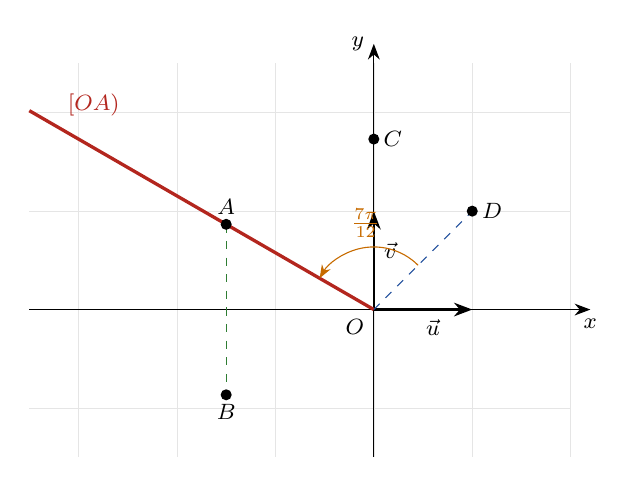
\begin{tikzpicture}[scale=1.25,font=\footnotesize]
\draw[gray!20,very thin] (-3.5,-1.5) grid (2,2.5);
\draw[-{Stealth[length=2mm]}] (-3.5,0)--(2.2,0) node[below]{$x$};
\draw[-{Stealth[length=2mm]}] (0,-1.5)--(0,2.7) node[left]{$y$};
\draw[-{Stealth},thick] (0,0)--(1,0) node[below,pos=0.6]{$\vec u$};
\draw[-{Stealth},thick] (0,0)--(0,1) node[right,pos=0.6]{$\vec v$};
\node[below left] at (0,0){$O$};
\draw[cThm,very thick] (0,0)--(-3.5,2.0207) node[above right,pos=0.92]{$[OA)$};
\draw[cDef,dashed] (0,0)--(1,1);
\draw[cRem,dashed] (-1.5,0.866)--(-1.5,-0.866);
\fill (-1.5,0.866) circle (1.6pt) node[above]{$A$};
\fill (-1.5,-0.866) circle (1.6pt) node[below]{$B$};
\fill (0,1.732) circle (1.6pt) node[right]{$C$};
\fill (1,1) circle (1.6pt) node[right]{$D$};
\draw[cEx,-{Stealth}] (0.45,0.45) arc (45:150:0.636) node[above,pos=0.5]{$\frac{7\pi}{12}$};
\end{tikzpicture}\end{LTR}\end{center}
\end{hal}

% ====================== التمرين: 2015 م2 ======================
\begin{tamrin}{بكالوريا 2015 -- الموضوع الثاني -- علوم تجريبية}
في المستوي المنسوب إلى المعلم المتعامد والمتجانس $(O;\vec u,\vec v)$ نعتبر النقط $A$، $B$ و$C$ التي لواحقها على الترتيب $z_A$، $z_B$ و$z_C$ حيث:
\[z_A=2e^{i\frac{\pi}{6}},\qquad z_B=-\overline{z_A},\qquad z_C=-(z_A+z_B).\]
\textbf{1)}
\begin{sq}
\qa اكتب كلًّا من العددين المركّبين $z_B$ و$z_C$ على الشكل الأسّي.
\qb استنتج أنّ النقط $A$، $B$ و$C$ تنتمي إلى دائرة $(\gamma)$ يُطلب تعيين مركزها ونصف قطرها.
\qc أنشئ الدائرة $(\gamma)$ والنقط $A$، $B$ و$C$.
\end{sq}
\textbf{2)}
\begin{sq}
\qa تحقّق أنّ: $\dfrac{z_B-z_C}{z_B-z_A}=e^{-i\frac{\pi}{3}}$.
\qb استنتج أنّ المثلث $ABC$ متقايس الأضلاع وأنّ النقطة $O$ مركز ثقل هذا المثلث.
\qc عيّن وأنشئ $(E)$ مجموعة النقط $M$ ذات اللاحقة $z$ حيث: $|z|=\left|z-\sqrt3-i\right|$.
\end{sq}
\textbf{3)}
\begin{sq}
\qa عيّن زاوية للدوران $r$ الذي مركزه $O$ ويحوّل $C$ إلى $A$.
\qb أثبت أنّ صورة $(E)$ بالدوران $r$ هي محور القطعة $[OB]$.
\end{sq}
\end{tamrin}

\begin{hal}
\QQ{1}
\pa $z_A=2\left(\cos\frac{\pi}{6}+i\sin\frac{\pi}{6}\right)=\sqrt3+i$، إذن $\overline{z_A}=\sqrt3-i$ و$z_B=-\overline{z_A}=-\sqrt3+i$.
\[|z_B|=\sqrt{3+1}=2,\quad \cos\theta=-\frac{\sqrt3}{2},\ \sin\theta=\frac12\ \Rightarrow\ \theta=\frac{5\pi}{6}:\qquad \bx{z_B=2e^{i\frac{5\pi}{6}}}\]
$z_C=-(z_A+z_B)=-(\sqrt3+i-\sqrt3+i)=-2i$، و$-i=e^{-i\frac{\pi}{2}}$:
\[\bx{z_C=2e^{-i\frac{\pi}{2}}}\]
\pb $OA=|z_A|=2$، $OB=|z_B|=2$، $OC=|z_C|=2$، إذن $OA=OB=OC=2$:
\bxt{$A$ و$B$ و$C$ تنتمي إلى الدائرة $(\gamma)$ التي مركزها $O$ ونصف قطرها $2$}
\pc الإنشاء: نرسم الدائرة $(\gamma)$، ثم نعلّم $A(\sqrt3;1)$ و$B(-\sqrt3;1)$ (على المستقيم $y=1$) و$C(0;-2)$ (انظر الشكل أسفله).

\QQ{2}
\pa $z_B-z_C=-\sqrt3+i+2i=-\sqrt3+3i$ و$z_B-z_A=-\sqrt3+i-\sqrt3-i=-2\sqrt3$، إذن:
\[\frac{z_B-z_C}{z_B-z_A}=\frac{-\sqrt3+3i}{-2\sqrt3}=\frac12-\frac{\sqrt3}{2}i=\cos\left(-\frac{\pi}{3}\right)+i\sin\left(-\frac{\pi}{3}\right)=\bx{e^{-i\frac{\pi}{3}}}\]
\pb من (أ): $\left|\dfrac{z_B-z_C}{z_B-z_A}\right|=1$ أي $\dfrac{BC}{BA}=1$ ومنه $BC=BA$، و$(\overrightarrow{BA};\overrightarrow{BC})=-\dfrac{\pi}{3}$ بترديد $2\pi$.
مثلث متساوي الساقين رأسه $B$ وزاوية رأسه $\dfrac{\pi}{3}$ فهو متقايس الأضلاع.
لاحقة مركز ثقله $G$: $z_G=\dfrac{z_A+z_B+z_C}{3}=\dfrac{z_A+z_B-(z_A+z_B)}{3}=0=z_O$.
\bxt{$ABC$ متقايس الأضلاع ومركز ثقله $O$}
\pc $|z|=|z-(\sqrt3+i)|\iff |z-z_O|=|z-z_A|\iff OM=AM$.
\bxt{$(E)$ هي محور القطعة $[OA]$}
للإنشاء: يشمل $(E)$ منتصف $[OA]$ ذا اللاحقة $\frac{\sqrt3}{2}+\frac12 i$ ويعامد $(OA)$؛ ويشمل أيضًا النقطتين ذواتي اللاحقتين $2i$ و$\sqrt3-i$ لأنّ: $|2i|=|2i-\sqrt3-i|=2$ و$|\sqrt3-i|=|-2i|=2$.

\QQ{3}
\pa الكتابة المركّبة للدوران $r$ الذي مركزه $O$ وزاويته $\theta$: $z'=e^{i\theta}z$. بما أنّ $r(C)=A$:
\[e^{i\theta}=\frac{z_A}{z_C}=\frac{2e^{i\frac{\pi}{6}}}{2e^{-i\frac{\pi}{2}}}=e^{i\left(\frac{\pi}{6}+\frac{\pi}{2}\right)}=e^{i\frac{2\pi}{3}}\qquad\Longrightarrow\qquad \bx{\theta=\frac{2\pi}{3}}\]
\pb $r(O)=O$، و$r(A)$ لاحقتها $e^{i\frac{2\pi}{3}}\cdot2e^{i\frac{\pi}{6}}=2e^{i\frac{5\pi}{6}}=z_B$ أي $r(A)=B$.
الدوران يحفظ المسافات: إذا كانت $M'=r(M)$ فإنّ $OM'=OM$ و$BM'=AM$. إذن:
\[M\in(E)\iff OM=AM\iff OM'=BM' ,\]
أي $M'$ تنتمي إلى محور القطعة $[OB]$، وبالعكس كل نقطة من محور $[OB]$ هي صورة نقطة من $(E)$ (الدوران تقابل).
\bxt{صورة $(E)$ بالدوران $r$ هي محور القطعة $[OB]$}

\begin{center}\begin{LTR}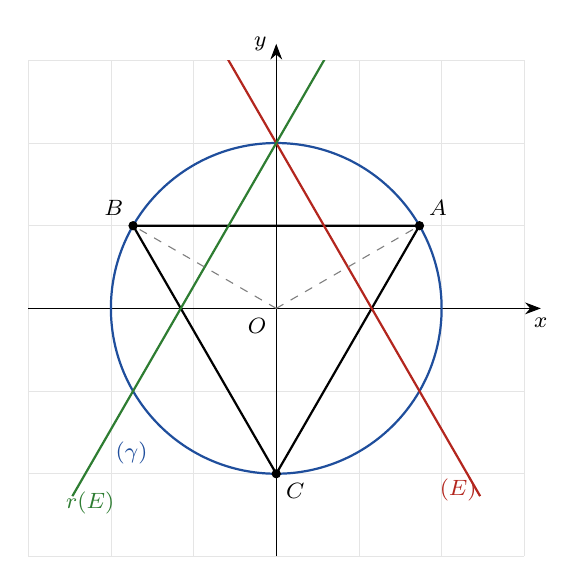
\begin{tikzpicture}[scale=1.05,font=\footnotesize]
\draw[gray!20,very thin] (-3,-3) grid (3,3);
\draw[-{Stealth[length=2mm]}] (-3,0)--(3.2,0) node[below]{$x$};
\draw[-{Stealth[length=2mm]}] (0,-3)--(0,3.2) node[left]{$y$};
\node[below left] at (0,0){$O$};
\draw[cDef,thick] (0,0) circle (2); \node[cDef] at (-1.75,-1.75){$(\gamma)$};
\draw[thick] (1.732,1)--(-1.732,1)--(0,-2)--cycle;
\clip (-3,-3) rectangle (3,3);
\draw[cThm,thick] ($(0.866,0.5)+1.6*(-1,1.732)$)--($(0.866,0.5)-1.6*(-1,1.732)$);
\node[cThm] at (2.2,-2.2){$(E)$};
\draw[cRem,thick] ($(-0.866,0.5)+1.6*(1,1.732)$)--($(-0.866,0.5)-1.6*(1,1.732)$);
\node[cRem] at (-2.25,-2.35){$r(E)$};
\draw[gray,dashed] (0,0)--(1.732,1) (0,0)--(-1.732,1);
\fill (1.732,1) circle (1.6pt) node[above right]{$A$};
\fill (-1.732,1) circle (1.6pt) node[above left]{$B$};
\fill (0,-2) circle (1.6pt) node[below right]{$C$};
\end{tikzpicture}\end{LTR}\end{center}
\end{hal}

% ====================== التمرين: 2014 م1 ======================
\begin{tamrin}{بكالوريا 2014 -- الموضوع الأول -- علوم تجريبية}
\textbf{1)} حلّ في مجموعة الأعداد المركّبة $\mathbb{C}$ المعادلة ذات المجهول $z$ التالية: $z^2-6\sqrt2\,z+36=0$.

\textbf{2)} المستوي المركّب منسوب إلى المعلم المتعامد والمتجانس $(O;\vec u,\vec v)$. لتكن النقط $A$، $B$، $C$ و$D$ لواحقها على الترتيب:
\[z_A=3\sqrt2(1+i),\qquad z_B=\overline{z_A},\qquad z_C=6\sqrt2,\qquad z_D=\frac{z_C}{2}.\]
\begin{sq}
\qa اكتب $z_A$، $z_B$ و$(1+i)z_A$ على الشكل الأسّي.
\qb احسب $\left(\dfrac{(1+i)z_A}{6\sqrt2}\right)^{2014}$.
\qc بيّن أنّ النقط $O$، $A$، $B$ و$C$ تنتمي إلى نفس الدائرة التي مركزها $D$، يُطلب تعيين نصف قطرها.
\qd احسب $\dfrac{z_B-z_C}{z_A-z_C}$ ثم جد قيسًا للزاوية $(\overrightarrow{CA};\overrightarrow{CB})$. ما هي طبيعة الرباعي $OACB$؟
\end{sq}
\textbf{3)} ليكن $R$ الدوران الذي مركزه $O$ وزاويته $\dfrac{\pi}{2}$.
\begin{sq}
\qa اكتب العبارة المركّبة للدوران $R$.
\qb عيّن لاحقة النقطة $C'$ صورة $C$ بالدوران $R$، ثم تحقّق أنّ النقط $A$، $C$ و$C'$ في استقامية.
\qc عيّن لاحقة النقطة $A'$ صورة $A$ بالدوران $R$، ثم حدّد صورة الرباعي $OACB$ بالدوران $R$.
\end{sq}
\end{tamrin}

\begin{hal}
\QQ{1}
$\Delta=(6\sqrt2)^2-4\times36=72-144=-72=\left(6\sqrt2\,i\right)^2$، فللمعادلة حلّان مركّبان مترافقان:
\[z_1=\frac{6\sqrt2-6\sqrt2\,i}{2}=3\sqrt2-3\sqrt2\,i,\qquad z_2=3\sqrt2+3\sqrt2\,i .\]
\[\bx{S=\left\{3\sqrt2-3\sqrt2\,i\,;\,3\sqrt2+3\sqrt2\,i\right\}}\]
\QQ{2}
\pa $1+i=\sqrt2\,e^{i\frac{\pi}{4}}$ إذن $z_A=3\sqrt2\cdot\sqrt2\,e^{i\frac{\pi}{4}}=6e^{i\frac{\pi}{4}}$، و$z_B=\overline{z_A}=6e^{-i\frac{\pi}{4}}$،
و$(1+i)z_A=\sqrt2\,e^{i\frac{\pi}{4}}\times6e^{i\frac{\pi}{4}}=6\sqrt2\,e^{i\frac{\pi}{2}}$.
\[\bx{z_A=6e^{i\frac{\pi}{4}}}\quad\bx{z_B=6e^{-i\frac{\pi}{4}}}\quad\bx{(1+i)z_A=6\sqrt2\,e^{i\frac{\pi}{2}}}\]
\pb $\dfrac{(1+i)z_A}{6\sqrt2}=e^{i\frac{\pi}{2}}$ إذن:
$\left(e^{i\frac{\pi}{2}}\right)^{2014}=e^{i\,1007\pi}=e^{i(503\times2\pi+\pi)}=e^{i\pi}$:
\[\bx{\left(\frac{(1+i)z_A}{6\sqrt2}\right)^{2014}=-1}\]
\pc $z_D=3\sqrt2$. نحسب المسافات:
\begin{align*}DO&=|0-3\sqrt2|=3\sqrt2, & DA&=|z_A-z_D|=|3\sqrt2\,i|=3\sqrt2,\\ DB&=|z_B-z_D|=|-3\sqrt2\,i|=3\sqrt2, & DC&=|6\sqrt2-3\sqrt2|=3\sqrt2 .\end{align*}
\bxt{$O$ و$A$ و$B$ و$C$ تنتمي إلى الدائرة التي مركزها $D$ ونصف قطرها $3\sqrt2$}
\pd $z_B-z_C=-3\sqrt2-3\sqrt2\,i=3\sqrt2(-1-i)$ و$z_A-z_C=-3\sqrt2+3\sqrt2\,i=3\sqrt2(-1+i)$، إذن:
\[\frac{z_B-z_C}{z_A-z_C}=\frac{-1-i}{-1+i}=\frac{(-1-i)(-1-i)}{(-1+i)(-1-i)}=\frac{1+2i+i^2}{2}=\bx{i}\]
ومنه $(\overrightarrow{CA};\overrightarrow{CB})=\arg(i)=\bx{\dfrac{\pi}{2}}$ بترديد $2\pi$، و$\dfrac{CB}{CA}=|i|=1$ أي $CA=CB$.

\textbf{طبيعة $OACB$:} منتصف القطر $[OC]$ لاحقته $\frac{0+6\sqrt2}{2}=3\sqrt2$، ومنتصف القطر $[AB]$ لاحقته $\frac{z_A+z_B}{2}=3\sqrt2$؛ للقطرين نفس المنتصف $D$ فالرباعي متوازي أضلاع، وفيه ضلعان متتاليان متقايسان ($CA=CB$) ومتعامدان، إذن:
\bxt{الرباعي $OACB$ مربّع}
\QQ{3}
\pa العبارة المركّبة للدوران الذي مركزه $O$ وزاويته $\frac{\pi}{2}$: $z'=e^{i\frac{\pi}{2}}z$ أي $\bx{z'=iz}$.
\pb $z_{C'}=i\,z_C=\bx{6\sqrt2\,i}$.
\[\frac{z_{C'}-z_A}{z_C-z_A}=\frac{-3\sqrt2+3\sqrt2\,i}{3\sqrt2-3\sqrt2\,i}=\frac{-(1-i)}{1-i}=-1\in\R\]
إذن الشعاعان $\overrightarrow{AC'}$ و$\overrightarrow{AC}$ مرتبطان خطيًا:
\bxt{النقط $A$ و$C$ و$C'$ في استقامية ($A$ منتصف $[CC']$)}
\pc $z_{A'}=i\,z_A=3\sqrt2(i+i^2)=\bx{-3\sqrt2+3\sqrt2\,i}$.
كذلك: $R(O)=O$، $R(C)=C'$، و$i\,z_B=3\sqrt2(i-i^2)=3\sqrt2+3\sqrt2\,i=z_A$ أي $R(B)=A$.
الدوران يحفظ الأطوال والزوايا فيحوّل المربّع إلى مربّع:
\bxt{صورة المربّع $OACB$ بالدوران $R$ هي المربّع $OA'C'A$}

\begin{center}\begin{LTR}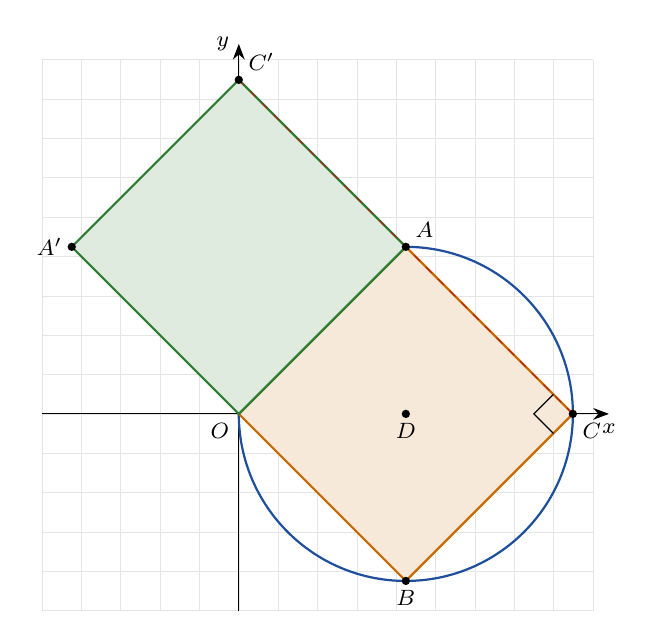
\begin{tikzpicture}[scale=0.5,font=\footnotesize]
\draw[gray!20,very thin] (-5,-5) grid (9,9);
\draw[-{Stealth[length=2mm]}] (-5,0)--(9.4,0) node[below]{$x$};
\draw[-{Stealth[length=2mm]}] (0,-5)--(0,9.4) node[left]{$y$};
\node[below left] at (0,0){$O$};
\draw[cDef,thick] (4.243,0) circle (4.243);
\fill[cEx!15] (0,0)--(4.243,4.243)--(8.485,0)--(4.243,-4.243)--cycle;
\draw[cEx,thick] (0,0)--(4.243,4.243)--(8.485,0)--(4.243,-4.243)--cycle;
\fill[cRem!15] (0,0)--(-4.243,4.243)--(0,8.485)--(4.243,4.243)--cycle;
\draw[cRem,thick] (0,0)--(-4.243,4.243)--(0,8.485)--(4.243,4.243)--cycle;
\draw[cThm,dashed] (8.485,0)--(0,8.485);
\draw (8.485,0) ++(135:0.7) -- ++(-135:0.7) -- ++(-45:0.7);
\fill (4.243,4.243) circle (3pt) node[above right]{$A$};
\fill (4.243,-4.243) circle (3pt) node[below]{$B$};
\fill (8.485,0) circle (3pt) node[below right]{$C$};
\fill (4.243,0) circle (3pt) node[below]{$D$};
\fill (0,8.485) circle (3pt) node[above right]{$C'$};
\fill (-4.243,4.243) circle (3pt) node[left]{$A'$};
\end{tikzpicture}\end{LTR}\end{center}
\end{hal}

% ====================== التمرين: 2014 م2 ======================
\begin{tamrin}{بكالوريا 2014 -- الموضوع الثاني -- علوم تجريبية}
\textbf{1)} حلّ في مجموعة الأعداد المركّبة $\mathbb{C}$ المعادلة ذات المجهول $z$ التالية: $(z-i)(z^2-2z+5)=0$.

\textbf{2)} في المستوي المنسوب إلى المعلم المتعامد والمتجانس $(O;\vec u,\vec v)$ (وحدة الطول $1\,\mathrm{cm}$) تُعطى النقط $A$، $B$ و$C$ لواحقها على الترتيب: $z_A=i$، $z_B=1+2i$، $z_C=1-2i$.
\begin{sq}
\qa أنشئ النقط $A$، $B$ و$C$.
\qb جد $z_H$ لاحقة النقطة $H$ المسقط العمودي للنقطة $A$ على $(BC)$.
\qc احسب مساحة المثلث $ABC$.
\end{sq}
\textbf{3)} ليكن $S$ التشابه المباشر الذي مركزه $A$ ونسبته $\dfrac12$ وزاويته $\dfrac{\pi}{2}$.
\begin{sq}
\qa عيّن الكتابة المركّبة للتشابه $S$.
\qb بيّن أنّ مساحة صورة المثلث $ABC$ بالتشابه $S$ تساوي $\dfrac12\,\mathrm{cm}^2$.
\end{sq}
\textbf{4)} $M$ نقطة لاحقتها $z$. عيّن مجموعة النقط $M$ حيث: $|z|=|iz+1+2i|$.
\end{tamrin}

\begin{hal}
\QQ{1}
$(z-i)(z^2-2z+5)=0\iff z-i=0$ أو $z^2-2z+5=0$.
\begin{itemize}
\item $z-i=0\iff z=i$.
\item $z^2-2z+5=0$: $\Delta=4-20=-16=(4i)^2$، إذن $z=\dfrac{2-4i}{2}=1-2i$ أو $z=1+2i$.
\end{itemize}
\[\bx{S=\{i\,;\,1-2i\,;\,1+2i\}}\]
\QQ{2}
\pa انظر الشكل أسفله: $A(0;1)$، $B(1;2)$، $C(1;-2)$.
\pb للنقطتين $B$ و$C$ نفس الجزء الحقيقي $1$، إذن $(BC)$ هو المستقيم الموازي لمحور التراتيب ذو المعادلة $x=1$.
المسقط العمودي لـ $A(0;1)$ على هذا المستقيم هو النقطة ذات الفاصلة $1$ والترتيبة $1$:
\[\bx{z_H=1+i}\]
تحقّق: $H\in(BC)$ لأنّ $\mathrm{Re}(z_H)=1$، و$\dfrac{z_H-z_A}{z_C-z_B}=\dfrac{1}{-4i}=\dfrac{i}{4}$ تخيّلي صرف، إذن $(AH)\perp(BC)$.
\pc $[AH]$ ارتفاع المثلث المتعلّق بالقاعدة $[BC]$: $BC=|z_C-z_B|=|-4i|=4$ و$AH=|z_H-z_A|=|1|=1$.
\[\mathcal{A}_{ABC}=\frac{BC\times AH}{2}=\frac{4\times1}{2}=\bx{2\ \mathrm{cm}^2}\]
\QQ{3}
\pa الكتابة المركّبة للتشابه المباشر الذي مركزه $A$ ونسبته $k$ وزاويته $\theta$: $z'-z_A=k\,e^{i\theta}(z-z_A)$، مع $\frac12 e^{i\frac{\pi}{2}}=\frac12 i$:
\[z'-i=\frac12 i\,(z-i)\iff z'=\frac12 iz-\frac12 i^2+i\iff \bx{z'=\frac12 iz+\frac12+i}\]
\pb التشابه الذي نسبته $k$ يضرب المساحات في $k^2$، فمساحة صورة المثلث $ABC$:
\[\mathcal{A}'=\left(\frac12\right)^2\times\mathcal{A}_{ABC}=\frac14\times2=\bx{\frac12\ \mathrm{cm}^2}\]
تحقّق مباشر: $S(A)=A$، $z_{B'}=\frac12 i(1+2i)+\frac12+i=-\frac12+\frac32 i$، $z_{C'}=\frac12 i(1-2i)+\frac12+i=\frac32+\frac32 i$؛
$B'C'=2$ والمسافة من $A(0;1)$ إلى المستقيم $y=\frac32$ هي $\frac12$، فالمساحة $\frac{2\times\frac12}{2}=\frac12$ \ok.
\QQ{4}
$iz+1+2i=i\left(z+\dfrac{1+2i}{i}\right)=i\,(z+2-i)$، و$|i|=1$، إذن $|iz+1+2i|=|z-(-2+i)|$.
لتكن $K$ النقطة ذات اللاحقة $z_K=-2+i$:
\[|z|=|iz+1+2i|\iff |z-z_O|=|z-z_K|\iff OM=KM .\]
\bxt{المجموعة $(\Delta)$ هي محور القطعة $[OK]$ حيث $z_K=-2+i$}
معادلته: $x^2+y^2=(x+2)^2+(y-1)^2\iff 4x-2y+5=0$، أي $y=2x+\frac52$.

\begin{center}\begin{LTR}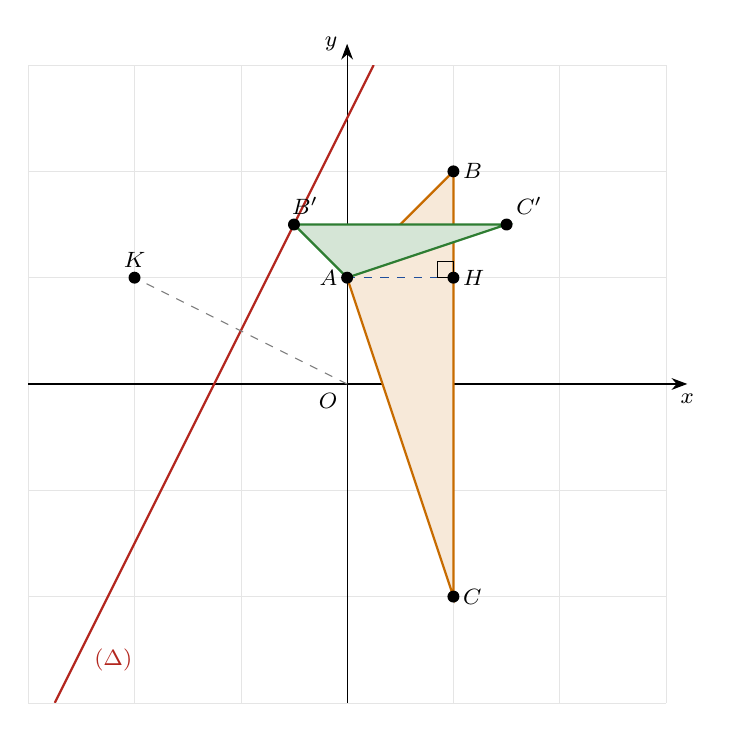
\begin{tikzpicture}[scale=1.35,font=\footnotesize]
\draw[gray!20,very thin] (-3,-3) grid (3,3);
\draw[-{Stealth[length=2mm]}] (-3,0)--(3.2,0) node[below]{$x$};
\draw[-{Stealth[length=2mm]}] (0,-3)--(0,3.2) node[left]{$y$};
\node[below left] at (0,0){$O$};
\fill[cEx!15] (0,1)--(1,2)--(1,-2)--cycle;
\draw[cEx,thick] (0,1)--(1,2)--(1,-2)--cycle;
\draw[cDef,dashed] (0,1)--(1,1);
\draw (1,1) rectangle (0.85,1.15);
\fill[cRem!20] (0,1)--(-0.5,1.5)--(1.5,1.5)--cycle;
\draw[cRem,thick] (0,1)--(-0.5,1.5)--(1.5,1.5)--cycle;
\begin{scope}\clip (-3,-3) rectangle (3,3);
\draw[cThm,thick] (-2.75,-3)--(0.25,3);\end{scope}
\node[cThm] at (-2.2,-2.6){$(\Delta)$};
\draw[gray,dashed] (0,0)--(-2,1);
\fill (0,1) circle (1.6pt) node[left]{$A$};
\fill (1,2) circle (1.6pt) node[right]{$B$};
\fill (1,-2) circle (1.6pt) node[right]{$C$};
\fill (1,1) circle (1.6pt) node[right]{$H$};
\fill (-0.5,1.5) circle (1.6pt) node[above,xshift=4pt]{$B'$};
\fill (1.5,1.5) circle (1.6pt) node[above right]{$C'$};
\fill (-2,1) circle (1.6pt) node[above]{$K$};
\end{tikzpicture}\end{LTR}\end{center}
\end{hal}
% ====================== التمرين: 2013 م1 ======================
\begin{tamrin}{بكالوريا 2013 -- الموضوع الأول -- علوم تجريبية}
\textbf{1)} حلّ في مجموعة الأعداد المركّبة $\mathbb{C}$ المعادلة $(I)$ ذات المجهول $z$ التالية:
\[z^2-(4\cos\alpha)z+4=0\qquad\ldots(I)\]
حيث $\alpha$ وسيط حقيقي.

\textbf{2)} من أجل $\alpha=\dfrac{\pi}{3}$، نرمز إلى حلّي المعادلة $(I)$ بـ $z_1$ و$z_2$. بيّن أنّ $\left(\dfrac{z_1}{z_2}\right)^{2013}=1$.

\textbf{3)} نعتبر في المستوي المنسوب إلى المعلم المتعامد والمتجانس $(O;\vec u,\vec v)$ النقط $A$، $B$ و$C$ التي لواحقها على الترتيب:
\[z_A=1+i\sqrt3,\qquad z_B=1-i\sqrt3,\qquad z_C=4+i\sqrt3 .\]
\begin{sq}
\qa أنشئ النقط $A$، $B$ و$C$.
\qb اكتب على الشكل الجبري العدد المركّب $\dfrac{z_C-z_A}{z_B-z_A}$، ثم استنتج أنّ $C$ هي صورة $B$ بالتشابه المباشر $S$ الذي مركزه $A$ ويُطلب تعيين نسبته وزاويته.
\qc عيّن لاحقة النقطة $G$ مرجح الجملة $\{(A;1),(B;-1),(C;2)\}$، ثم أنشئ $G$.
\qd احسب $z_D$ لاحقة النقطة $D$ بحيث يكون الرباعي $ABDG$ متوازي أضلاع.
\end{sq}
\end{tamrin}

\begin{hal}
\QQ{1}
$\Delta=(4\cos\alpha)^2-4\times4=16\cos^2\alpha-16=-16(1-\cos^2\alpha)=-16\sin^2\alpha=(4i\sin\alpha)^2$.
إذن حلّا المعادلة (وهما متساويان إذا كان $\sin\alpha=0$):
\[z_1=\frac{4\cos\alpha+4i\sin\alpha}{2}=2(\cos\alpha+i\sin\alpha),\qquad z_2=\frac{4\cos\alpha-4i\sin\alpha}{2}=2(\cos\alpha-i\sin\alpha).\]
\[\bx{S=\left\{2e^{i\alpha}\,;\,2e^{-i\alpha}\right\}}\]
\QQ{2}
من أجل $\alpha=\frac{\pi}{3}$: $z_1=2e^{i\frac{\pi}{3}}=1+i\sqrt3$ و$z_2=2e^{-i\frac{\pi}{3}}=1-i\sqrt3$، إذن $\dfrac{z_1}{z_2}=e^{i\frac{2\pi}{3}}$ ومنه:
\[\left(\frac{z_1}{z_2}\right)^{2013}=e^{i\frac{2\times2013\,\pi}{3}}=e^{i\,1342\pi}=e^{i\,(671\times2\pi)}=\bx{1}\]
(النتيجة نفسها لو بدّلنا تسمية الحلّين لأنّ $\left(e^{-i\frac{2\pi}{3}}\right)^{2013}=e^{-i1342\pi}=1$.)
\QQ{3}
\pa انظر الشكل أسفله: $A(1;\sqrt3)$، $B(1;-\sqrt3)$، $C(4;\sqrt3)$ مع $\sqrt3\approx1{,}73$.
\pb $z_C-z_A=3$ و$z_B-z_A=-2i\sqrt3$، إذن:
\[\frac{z_C-z_A}{z_B-z_A}=\frac{3}{-2i\sqrt3}=\frac{3i}{-2i^2\sqrt3}=\frac{3i}{2\sqrt3}=\bx{\frac{\sqrt3}{2}\,i}\]
ومنه $z_C-z_A=\dfrac{\sqrt3}{2}e^{i\frac{\pi}{2}}(z_B-z_A)$، وهذه هي العلاقة $z'-z_A=k e^{i\theta}(z-z_A)$ للتشابه المباشر الذي مركزه $A$ مطبّقة على $B$:
\bxt{$C=S(B)$ حيث $S$ تشابه مباشر مركزه $A$ نسبته $\frac{\sqrt3}{2}$ وزاويته $\frac{\pi}{2}$}
\pc مجموع المعاملات $1-1+2=2\neq0$ فالمرجح موجود:
\[z_G=\frac{z_A-z_B+2z_C}{2}=\frac{2i\sqrt3+8+2i\sqrt3}{2}=\bx{4+2i\sqrt3}\]
للإنشاء: $z_G-z_C=4+2i\sqrt3-4-i\sqrt3=i\sqrt3=\frac12(z_A-z_B)$، أي $\overrightarrow{CG}=\frac12\overrightarrow{BA}$.
\pd $ABDG$ متوازي أضلاع $\iff\overrightarrow{AB}=\overrightarrow{GD}\iff z_B-z_A=z_D-z_G$، إذن:
\[z_D=z_G+z_B-z_A=4+2i\sqrt3-2i\sqrt3=\bx{4}\]

\begin{center}\begin{LTR}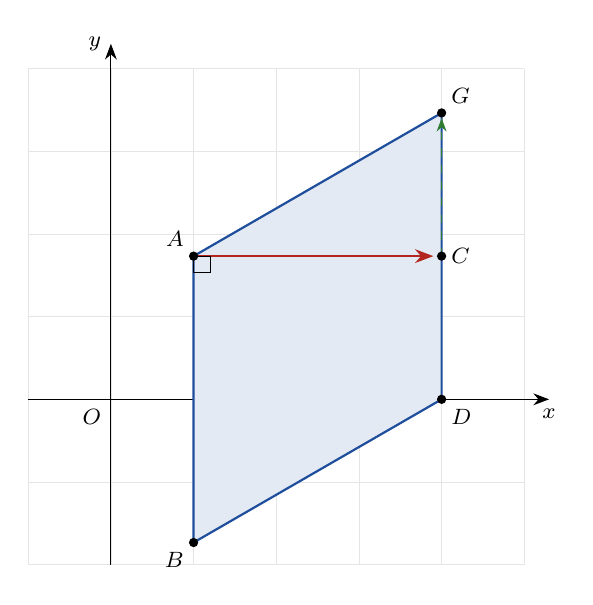
\begin{tikzpicture}[scale=1.05,font=\footnotesize]
\draw[gray!20,very thin] (-1,-2) grid (5,4);
\draw[-{Stealth[length=2mm]}] (-1,0)--(5.3,0) node[below]{$x$};
\draw[-{Stealth[length=2mm]}] (0,-2)--(0,4.3) node[left]{$y$};
\node[below left] at (0,0){$O$};
\fill[cDef!12] (1,1.732)--(1,-1.732)--(4,0)--(4,3.464)--cycle;
\draw[cDef,thick] (1,1.732)--(1,-1.732)--(4,0)--(4,3.464)--cycle;
\draw[cThm,thick,-{Stealth}] (1,1.732)--(3.9,1.732);
\draw (1,1.732) rectangle (1.2,1.532);
\draw[cRem,dashed,-{Stealth}] (4,1.732)--(4,3.4);
\fill (1,1.732) circle (1.6pt) node[above left]{$A$};
\fill (1,-1.732) circle (1.6pt) node[below left]{$B$};
\fill (4,1.732) circle (1.6pt) node[right]{$C$};
\fill (4,3.464) circle (1.6pt) node[above right]{$G$};
\fill (4,0) circle (1.6pt) node[below right]{$D$};
\end{tikzpicture}\end{LTR}\end{center}
\end{hal}

% ====================== التمرين: 2013 م2 ======================
\begin{tamrin}{بكالوريا 2013 -- الموضوع الثاني -- علوم تجريبية}
نعتبر في مجموعة الأعداد المركّبة $\mathbb{C}$ المعادلة $(E)$ ذات المجهول $z$ الآتية:
\[z^2+4z+13=0\qquad\ldots(E)\]
\textbf{1)} تحقّق أنّ العدد المركّب $-2-3i$ حلّ للمعادلة $(E)$، ثم جد الحلّ الآخر.

\textbf{2)} $A$ و$B$ نقطتان من المستوي المركّب لاحقتاهما $z_A=-2-3i$ و$z_B=i$ على الترتيب.
$S$ التشابه المباشر الذي مركزه $A$، نسبته $\dfrac12$ وزاويته $\dfrac{\pi}{2}$ والذي يحوّل كلّ نقطة $M(z)$ من المستوي إلى النقطة $M'(z')$.
\begin{sq}
\qa بيّن أنّ: $z'=\dfrac12 iz-\dfrac72-2i$.
\qb احسب $z_C$ لاحقة النقطة $C$، علمًا أنّ $C$ هي صورة $B$ بالتشابه $S$.
\end{sq}
\textbf{3)} لتكن النقطة $D$ حيث: $2\overrightarrow{AD}+\overrightarrow{AB}=\vec 0$.
\begin{sq}
\qa بيّن أنّ $D$ مرجح النقطتين $A$ و$B$ المرفقتين بمعاملين حقيقيين يُطلب تعيينهما.
\qb احسب $z_D$ لاحقة النقطة $D$.
\qc بيّن أنّ $\dfrac{z_D-z_A}{z_C-z_A}=i$، ثم استنتج طبيعة المثلث $ACD$.
\end{sq}
\end{tamrin}

\begin{hal}
\QQ{1}
$(-2-3i)^2=4+12i+9i^2=-5+12i$، إذن:
\[(-2-3i)^2+4(-2-3i)+13=-5+12i-8-12i+13=0 .\]
\bxt{$-2-3i$ حلّ للمعادلة $(E)$}
مجموع الحلّين $z_1+z_2=-\dfrac{b}{a}=-4$، إذن الحلّ الآخر: $z_2=-4-(-2-3i)=\bx{-2+3i}$ (وهو مرافق الأول لأنّ المعاملات حقيقية).
\QQ{2}
\pa الكتابة المركّبة للتشابه المباشر الذي مركزه $A$ ونسبته $\frac12$ وزاويته $\frac{\pi}{2}$:
$z'-z_A=\frac12 e^{i\frac{\pi}{2}}(z-z_A)=\frac12 i\,(z-z_A)$، أي $z'=\frac12 iz+z_A\left(1-\frac12 i\right)$. نحسب:
\[(-2-3i)\left(1-\frac12 i\right)=-2+i-3i+\frac32 i^2=-2-2i-\frac32=-\frac72-2i .\]
\[\bx{z'=\frac12 iz-\frac72-2i}\]
\pb $z_C=\frac12 i\times i-\frac72-2i=-\frac12-\frac72-2i$:
\[\bx{z_C=-4-2i}\]
\QQ{3}
\pa حسب علاقة شال: $\overrightarrow{AB}=\overrightarrow{AD}+\overrightarrow{DB}$، إذن:
\[2\overrightarrow{AD}+\overrightarrow{AD}+\overrightarrow{DB}=\vec0\iff 3\overrightarrow{AD}+\overrightarrow{DB}=\vec0\iff 3\overrightarrow{DA}-\overrightarrow{DB}=\vec0 .\]
بما أنّ $3+(-1)=2\neq0$:
\bxt{$D$ مرجح الجملة $\{(A;3),(B;-1)\}$}
\pb $z_D=\dfrac{3z_A-z_B}{3-1}=\dfrac{-6-9i-i}{2}$:
\[\bx{z_D=-3-5i}\]
\pc $z_D-z_A=-1-2i$ و$z_C-z_A=-2+i$:
\[\frac{z_D-z_A}{z_C-z_A}=\frac{-1-2i}{-2+i}=\frac{(-1-2i)(-2-i)}{(-2)^2+1^2}=\frac{2+i+4i+2i^2}{5}=\frac{5i}{5}=\bx{i}\]
إذن:
\[\frac{AD}{AC}=|i|=1\ \Rightarrow\ AD=AC,\qquad (\overrightarrow{AC};\overrightarrow{AD})=\arg(i)=\frac{\pi}{2}\ [2\pi].\]
\bxt{المثلث $ACD$ قائم ومتساوي الساقين في $A$}

\begin{center}\begin{LTR}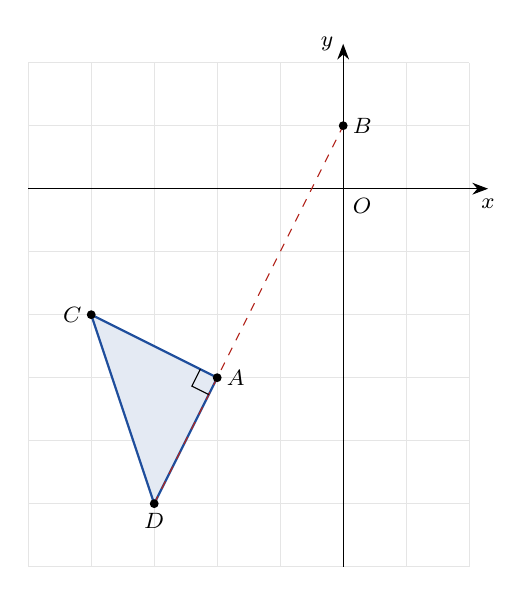
\begin{tikzpicture}[scale=0.8,font=\footnotesize]
\draw[gray!20,very thin] (-5,-6) grid (2,2);
\draw[-{Stealth[length=2mm]}] (-5,0)--(2.3,0) node[below]{$x$};
\draw[-{Stealth[length=2mm]}] (0,-6)--(0,2.3) node[left]{$y$};
\node[below right] at (0,0){$O$};
\fill[cDef!12] (-2,-3)--(-4,-2)--(-3,-5)--cycle;
\draw[cDef,thick] (-2,-3)--(-4,-2)--(-3,-5)--cycle;
\draw[cThm,dashed] (-3,-5)--(0,1);
\draw (-2.268,-2.866)--(-2.402,-3.134)--(-2.134,-3.268);
\fill (-2,-3) circle (2pt) node[right]{$A$};
\fill (0,1) circle (2pt) node[right]{$B$};
\fill (-4,-2) circle (2pt) node[left]{$C$};
\fill (-3,-5) circle (2pt) node[below]{$D$};
\end{tikzpicture}\end{LTR}\end{center}
\end{hal}

% ====================== التمرين: 2012 م1 ======================
\begin{tamrin}{بكالوريا 2012 -- الموضوع الأول -- علوم تجريبية}
\textbf{1)} نعتبر في مجموعة الأعداد المركّبة $\mathbb{C}$ المعادلة ذات المجهول $z$:
$z=\dfrac{3i(z+2i)}{z-2+3i}$ (حيث $z\neq2-3i$).
\begin{itemize}
\item حلّ في $\mathbb{C}$ هذه المعادلة.
\end{itemize}
\textbf{2)} ينسب المستوي المركّب إلى المعلم المتعامد والمتجانس $(O;\vec u,\vec v)$. $A$، $B$ نقطتان لاحقتاهما على الترتيب $z_A$ و$z_B$ حيث: $z_A=1+i\sqrt5$ و$z_B=1-i\sqrt5$.
\begin{itemize}
\item تحقّق أنّ $A$ و$B$ تنتميان إلى دائرة مركزها $O$ يُطلب تعيين نصف قطرها.
\end{itemize}
\textbf{3)} نرفق بكلّ نقطة $M$ من المستوي لاحقتها $z$ ($z\neq2-3i$) النقطة $M'$ لاحقتها $z'$ حيث: $z'=\dfrac{3i(z+2i)}{z-2+3i}$.
النقط $C$، $D$، $E$ لواحقها على الترتيب: $z_C=-2i$، $z_D=2-3i$ و$z_E=3i$، و$(\Delta)$ محور القطعة $[CD]$.
\begin{sq}
\qa عبّر عن المسافة $OM'$ بدلالة المسافتين $CM$ و$DM$.
\qb استنتج أنّه من أجل كلّ نقطة $M$ من $(\Delta)$ فإنّ النقطة $M'$ تنتمي إلى دائرة $(\gamma)$ يُطلب تعيين مركزها ونصف قطرها. تحقّق أنّ $E$ تنتمي إلى $(\gamma)$.
\end{sq}
\end{tamrin}

\begin{hal}
\QQ{1}
من أجل $z\neq2-3i$:
\[z=\frac{3i(z+2i)}{z-2+3i}\iff z(z-2+3i)=3iz+6i^2\iff z^2-2z+3iz=3iz-6\iff z^2-2z+6=0 .\]
$\Delta=4-24=-20=\left(2i\sqrt5\right)^2$، إذن $z=\dfrac{2\pm2i\sqrt5}{2}=1\pm i\sqrt5$، وكلاهما يختلف عن $2-3i$:
\[\bx{S=\left\{1-i\sqrt5\,;\,1+i\sqrt5\right\}}\]
\QQ{2}
\[OA=|z_A|=\sqrt{1^2+(\sqrt5)^2}=\sqrt6,\qquad OB=|z_B|=\sqrt{1^2+(-\sqrt5)^2}=\sqrt6 .\]
\bxt{$A$ و$B$ تنتميان إلى الدائرة التي مركزها $O$ ونصف قطرها $\sqrt6$}
\QQ{3}
\pa $OM'=|z'|=\dfrac{|3i|\cdot|z+2i|}{|z-2+3i|}=\dfrac{3\,|z-(-2i)|}{|z-(2-3i)|}=\dfrac{3\,|z-z_C|}{|z-z_D|}$:
\[\bx{OM'=\frac{3\,CM}{DM}}\]
\pb إذا كانت $M\in(\Delta)$ فإنّ $CM=DM$، مع $DM\neq0$ لأنّ $D\notin(\Delta)$.\par إذن $OM'=\dfrac{3\,CM}{DM}=3$:
\bxt{$M'$ تنتمي إلى الدائرة $(\gamma)$ التي مركزها $O$ ونصف قطرها $3$}
$OE=|z_E|=|3i|=3$ إذن \bxt{$E\in(\gamma)$}.

\begin{center}\begin{LTR}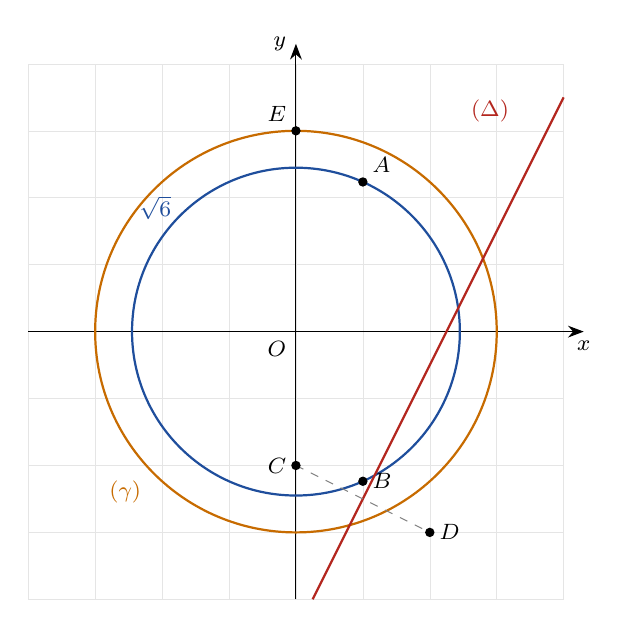
\begin{tikzpicture}[scale=0.85,font=\footnotesize]
\draw[gray!20,very thin] (-4,-4) grid (4,4);
\draw[-{Stealth[length=2mm]}] (-4,0)--(4.3,0) node[below]{$x$};
\draw[-{Stealth[length=2mm]}] (0,-4)--(0,4.3) node[left]{$y$};
\node[below left] at (0,0){$O$};
\draw[cDef,thick] (0,0) circle (2.449);
\node[cDef] at (-2.1,1.85){$\sqrt6$};
\draw[cEx,thick] (0,0) circle (3); \node[cEx] at (-2.55,-2.4){$(\gamma)$};
\draw[cThm,thick] (0.25,-4)--(4,3.5); \node[cThm] at (2.9,3.3){$(\Delta)$};
\draw[gray,dashed] (0,-2)--(2,-3);
\fill (1,2.236) circle (2pt) node[above right]{$A$};
\fill (1,-2.236) circle (2pt) node[right]{$B$};
\fill (0,-2) circle (2pt) node[left]{$C$};
\fill (2,-3) circle (2pt) node[right]{$D$};
\fill (0,3) circle (2pt) node[above left]{$E$};
\end{tikzpicture}\end{LTR}\end{center}
\end{hal}

% ====================== التمرين: 2012 م2 ======================
\begin{tamrin}{بكالوريا 2012 -- الموضوع الثاني -- علوم تجريبية}
\textbf{1)} $P(z)$ كثير حدود للمتغيّر المركّب $z$ حيث: $P(z)=z^3-12z^2+48z-72$.
\begin{sq}
\qa تحقّق أنّ $6$ هو جذر لكثير الحدود $P(z)$.
\qb حدّد العددين الحقيقيين $\alpha$ و$\beta$ بحيث من أجل كلّ عدد مركّب $z$: $P(z)=(z-6)(z^2+\alpha z+\beta)$.
\qc حلّ في مجموعة الأعداد المركّبة $\mathbb{C}$ المعادلة $P(z)=0$.
\end{sq}
\textbf{2)} المستوي المركّب منسوب إلى المعلم المتعامد والمتجانس $(O;\vec u,\vec v)$. $A$، $B$ و$C$ نقط من المستوي المركّب لواحقها على الترتيب:
\[z_A=6,\qquad z_B=3+i\sqrt3,\qquad z_C=3-i\sqrt3 .\]
\begin{sq}
\qa اكتب كلًّا من $z_A$، $z_B$ و$z_C$ على الشكل الأسّي.
\qb اكتب العدد المركّب $\dfrac{z_A-z_B}{z_A-z_C}$ على الشكل الجبري، ثم على الشكل الأسّي.
\qc استنتج طبيعة المثلث $ABC$.
\end{sq}
\textbf{3)} ليكن $S$ التشابه المباشر الذي مركزه $C$، نسبته $\sqrt3$ وزاويته $\dfrac{\pi}{2}$.
\begin{sq}
\qa جد الكتابة المركّبة للتشابه $S$.
\qb عيّن $z_{A'}$ لاحقة النقطة $A'$ صورة النقطة $A$ بالتشابه $S$.
\qc بيّن أنّ النقط $A$، $B$ و$A'$ في استقامية.
\end{sq}
\end{tamrin}

\begin{hal}
\QQ{1}
\pa $P(6)=216-12\times36+48\times6-72=216-432+288-72=\bx{0}$، إذن $6$ جذر لـ $P(z)$.
\pb ننشر: $(z-6)(z^2+\alpha z+\beta)=z^3+(\alpha-6)z^2+(\beta-6\alpha)z-6\beta$. بالمطابقة مع $P(z)$:
\[\begin{cases}\alpha-6=-12\\ \beta-6\alpha=48\\ -6\beta=-72\end{cases}\iff\begin{cases}\alpha=-6\\ \beta=12\end{cases}\]
(تحقّق: $\beta-6\alpha=12+36=48$ \ok).
\[\bx{P(z)=(z-6)(z^2-6z+12)}\]
\pc $P(z)=0\iff z=6$ أو $z^2-6z+12=0$؛ $\Delta=36-48=-12=\left(2i\sqrt3\right)^2$، ومنه $z=\dfrac{6\pm2i\sqrt3}{2}=3\pm i\sqrt3$:
\[\bx{S=\left\{6\,;\,3-i\sqrt3\,;\,3+i\sqrt3\right\}}\]
\QQ{2}
\pa $z_A=6=6e^{i0}$. $|z_B|=\sqrt{9+3}=2\sqrt3$، و$\cos\theta=\dfrac{3}{2\sqrt3}=\dfrac{\sqrt3}{2}$، $\sin\theta=\dfrac{\sqrt3}{2\sqrt3}=\dfrac12$، إذن $\theta=\dfrac{\pi}{6}$؛ و$z_C=\overline{z_B}$:
\[\bx{z_A=6e^{i0}}\qquad\bx{z_B=2\sqrt3\,e^{i\frac{\pi}{6}}}\qquad\bx{z_C=2\sqrt3\,e^{-i\frac{\pi}{6}}}\]
\pb
\[\frac{z_A-z_B}{z_A-z_C}=\frac{3-i\sqrt3}{3+i\sqrt3}=\frac{(3-i\sqrt3)^2}{9+3}=\frac{9-6i\sqrt3-3}{12}=\bx{\frac12-\frac{\sqrt3}{2}i}=\bx{e^{-i\frac{\pi}{3}}}\]
\pc $\left|\dfrac{z_A-z_B}{z_A-z_C}\right|=1$ إذن $AB=AC$، و$(\overrightarrow{AC};\overrightarrow{AB})=-\dfrac{\pi}{3}$ بترديد $2\pi$:
\bxt{المثلث $ABC$ متقايس الأضلاع}
\QQ{3}
\pa $z'-z_C=\sqrt3\,e^{i\frac{\pi}{2}}(z-z_C)=i\sqrt3\,(z-z_C)$، أي $z'=i\sqrt3\,z+z_C(1-i\sqrt3)$، و:
\[(3-i\sqrt3)(1-i\sqrt3)=3-3i\sqrt3-i\sqrt3+3i^2=-4i\sqrt3 .\]
\[\bx{z'=i\sqrt3\,z-4i\sqrt3}\]
\pb $z_{A'}=i\sqrt3\times6-4i\sqrt3=\bx{2i\sqrt3}$.
\pc $z_{A'}-z_A=-6+2i\sqrt3$ و$z_B-z_A=-3+i\sqrt3$، إذن:
\[\frac{z_{A'}-z_A}{z_B-z_A}=\frac{2(-3+i\sqrt3)}{-3+i\sqrt3}=2\in\R\]
\bxt{النقط $A$ و$B$ و$A'$ في استقامية ($B$ منتصف $[AA']$)}

\begin{center}\begin{LTR}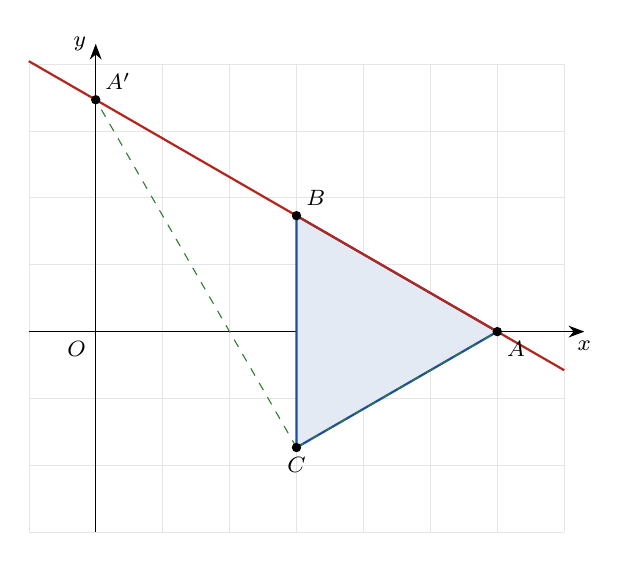
\begin{tikzpicture}[scale=0.85,font=\footnotesize]
\draw[gray!20,very thin] (-1,-3) grid (7,4);
\draw[-{Stealth[length=2mm]}] (-1,0)--(7.3,0) node[below]{$x$};
\draw[-{Stealth[length=2mm]}] (0,-3)--(0,4.3) node[left]{$y$};
\node[below left] at (0,0){$O$};
\fill[cDef!12] (6,0)--(3,1.732)--(3,-1.732)--cycle;
\draw[cDef,thick] (6,0)--(3,1.732)--(3,-1.732)--cycle;
\draw[cThm,thick] (7,-0.577)--(-1,4.041);
\draw[cRem,dashed] (3,-1.732)--(6,0) (3,-1.732)--(0,3.464);
\fill (6,0) circle (2pt) node[below right]{$A$};
\fill (3,1.732) circle (2pt) node[above right]{$B$};
\fill (3,-1.732) circle (2pt) node[below]{$C$};
\fill (0,3.464) circle (2pt) node[above right]{$A'$};
\end{tikzpicture}\end{LTR}\end{center}
\end{hal}

% ====================== التمرين: 2011 م1 ======================
\begin{tamrin}{بكالوريا 2011 -- الموضوع الأول -- علوم تجريبية}
نعتبر في المستوي المنسوب إلى المعلم المتعامد والمتجانس $(O;\vec u,\vec v)$ النقط $A$، $B$ و$C$ لواحقها على الترتيب:
\[z_A=-i,\qquad z_B=2+3i,\qquad z_C=-4+i .\]
\textbf{1)}
\begin{sq}
\qa اكتب على الشكل الجبري العدد المركّب $\dfrac{z_C-z_A}{z_B-z_A}$.
\qb عيّن طويلة العدد المركّب $\dfrac{z_C-z_A}{z_B-z_A}$ وعمدة له، ثم استنتج طبيعة المثلث $ABC$.
\end{sq}
\textbf{2)} نعتبر التحويل النقطي $T$ في المستوي الذي يرفق بكلّ نقطة $M$ لاحقتها $z$ النقطة $M'$ ذات اللاحقة $z'$ بحيث: $z'=iz-1-i$.
\begin{sq}
\qa عيّن طبيعة التحويل $T$ محدّدًا عناصره المميّزة.
\qb ما هي صورة النقطة $B$ بالتحويل $T$؟
\end{sq}
\textbf{3)} لتكن $D$ ذات اللاحقة $z_D=-6+2i$.
\begin{sq}
\qa بيّن أنّ النقط $A$، $C$ و$D$ في استقامية.
\qb عيّن نسبة التحاكي $h$ الذي مركزه $A$ ويحوّل النقطة $C$ إلى $D$.
\qc عيّن العناصر المميّزة للتشابه المباشر $S$ الذي مركزه $A$ ويحوّل $B$ إلى $D$.
\end{sq}
\end{tamrin}

\begin{hal}
\QQ{1}
\pa $z_C-z_A=-4+2i$ و$z_B-z_A=2+4i$:
\[\frac{z_C-z_A}{z_B-z_A}=\frac{(-4+2i)(2-4i)}{(2+4i)(2-4i)}=\frac{-8+16i+4i-8i^2}{4+16}=\frac{20i}{20}=\bx{i}\]
\pb $|i|=1$ و$\arg(i)=\dfrac{\pi}{2}$ بترديد $2\pi$. إذن:
\[\frac{AC}{AB}=1\ \Rightarrow\ AB=AC,\qquad (\overrightarrow{AB};\overrightarrow{AC})=\frac{\pi}{2}\ [2\pi].\]
\bxt{المثلث $ABC$ قائم ومتساوي الساقين في $A$}
\QQ{2}
\pa $z'=az+b$ مع $a=i$: $|a|=1$ و$a\neq1$، فـ $T$ دوران زاويته $\arg(i)=\frac{\pi}{2}$. مركزه $\omega$ النقطة الصامدة:
\begin{align*}\omega=i\omega-1-i&\iff\omega(1-i)=-1-i\\&\iff\omega=\frac{-1-i}{1-i}=\frac{(-1-i)(1+i)}{2}=\frac{-1-2i-i^2}{2}=-i=z_A .\end{align*}
\bxt{$T$ دوران مركزه $A$ وزاويته $\frac{\pi}{2}$}
\pb $z_{B'}=i(2+3i)-1-i=2i-3-1-i=-4+i=z_C$:
\bxt{صورة $B$ بالتحويل $T$ هي النقطة $C$}
(وهذا يوافق نتيجة السؤال 1: $AC=AB$ و$(\overrightarrow{AB};\overrightarrow{AC})=\frac{\pi}{2}$.)
\QQ{3}
\pa $z_D-z_A=-6+3i$ و$z_C-z_A=-4+2i$، إذن:
\[\frac{z_D-z_A}{z_C-z_A}=\frac{3(-2+i)}{2(-2+i)}=\frac32\in\R\]
\bxt{النقط $A$ و$C$ و$D$ في استقامية}
\pb $h(C)=D\iff z_D-z_A=k(z_C-z_A)$، ومن (أ): $\bx{k=\dfrac32}$.
\pc $\dfrac{z_D-z_A}{z_B-z_A}=\dfrac{-6+3i}{2+4i}=\dfrac{(-6+3i)(2-4i)}{20}=\dfrac{-12+24i+6i-12i^2}{20}=\dfrac{30i}{20}=\dfrac32 i=\dfrac32 e^{i\frac{\pi}{2}}$.
إذن $z_D-z_A=\frac32 e^{i\frac{\pi}{2}}(z_B-z_A)$:
\bxt{$S$ تشابه مباشر مركزه $A$ نسبته $\frac32$ وزاويته $\frac{\pi}{2}$}
كتابته المركّبة: $z'+i=\frac32 i(z+i)$ أي $z'=\frac32 iz-\frac32-i$، ونلاحظ أنّ $S=h\circ T$.

\begin{center}\begin{LTR}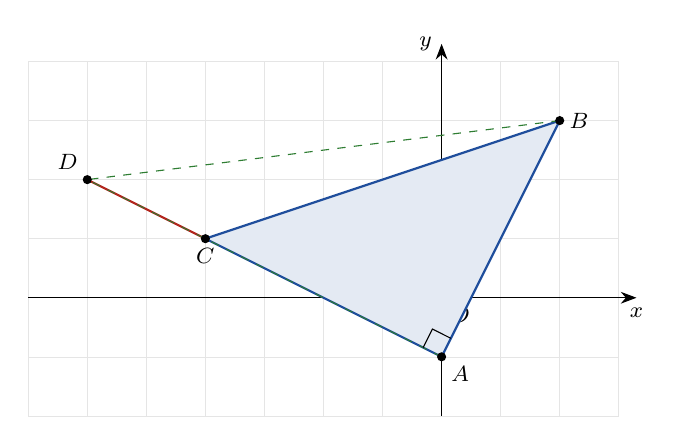
\begin{tikzpicture}[scale=0.75,font=\footnotesize]
\draw[gray!20,very thin] (-7,-2) grid (3,4);
\draw[-{Stealth[length=2mm]}] (-7,0)--(3.3,0) node[below]{$x$};
\draw[-{Stealth[length=2mm]}] (0,-2)--(0,4.3) node[left]{$y$};
\node[below right] at (0,0){$O$};
\fill[cDef!12] (0,-1)--(2,3)--(-4,1)--cycle;
\draw[cDef,thick] (0,-1)--(2,3)--(-4,1)--cycle;
\draw[cThm,thick] (-4,1)--(-6,2);
\draw[cRem,dashed] (0,-1)--(-6,2) (2,3)--(-6,2);
\draw (0.157,-0.687)--(-0.156,-0.530)--(-0.313,-0.843);
\fill (0,-1) circle (2.2pt) node[below right]{$A$};
\fill (2,3) circle (2.2pt) node[right]{$B$};
\fill (-4,1) circle (2.2pt) node[below]{$C$};
\fill (-6,2) circle (2.2pt) node[above left]{$D$};
\end{tikzpicture}\end{LTR}\end{center}
\end{hal}
% ====================== التمرين: 2011 م2 ======================
\begin{tamrin}{بكالوريا 2011 -- الموضوع الثاني -- علوم تجريبية}
نعتبر في المستوي المنسوب إلى المعلم المتعامد والمتجانس $(O;\vec u,\vec v)$ النقط $A$، $B$ و$C$ لواحقها على الترتيب:
\[z_A=3-2i,\qquad z_B=3+2i,\qquad z_C=4i .\]
\textbf{1)}
\begin{sq}
\qa علّم النقط $A$، $B$ و$C$.
\qb ما هي طبيعة الرباعي $OABC$؟ علّل إجابتك.
\qc عيّن لاحقة النقطة $\Omega$ مركز الرباعي $OABC$.
\end{sq}
\textbf{2)} عيّن ثم أنشئ $(E)$ مجموعة النقط $M$ من المستوي التي تحقّق: $\left\|\overrightarrow{MO}+\overrightarrow{MA}+\overrightarrow{MB}+\overrightarrow{MC}\right\|=12$.

\textbf{3)}
\begin{sq}
\qa حلّ في مجموعة الأعداد المركّبة $\mathbb{C}$ المعادلة: $z^2-6z+13=0$. نسمّي $z_0$، $z_1$ حلّي هذه المعادلة.
\qb لتكن $M$ نقطة من المستوي لاحقتها العدد المركّب $z$. عيّن مجموعة النقط $M$ من المستوي التي تحقّق: $|z-z_0|=|z-z_1|$.
\end{sq}
\end{tamrin}

\begin{hal}
\QQ{1}
\pa $A(3;-2)$، $B(3;2)$، $C(0;4)$ (انظر الشكل أسفله).
\pb لاحقة الشعاع $\overrightarrow{OA}$ هي $z_A-z_O=3-2i$، ولاحقة الشعاع $\overrightarrow{CB}$ هي $z_B-z_C=3+2i-4i=3-2i$.
إذن $\overrightarrow{OA}=\overrightarrow{CB}$:
\bxt{الرباعي $OABC$ متوازي أضلاع}
(ليس معيّنًا لأنّ $OA=\sqrt{13}$ و$AB=|4i|=4$، وليس مستطيلًا لأنّ القطرين غير متقايسين: $OB=\sqrt{13}$ و$AC=|-3+6i|=3\sqrt5$.)
\pc مركز متوازي الأضلاع هو منتصف قطره $[OB]$:
\[z_\Omega=\frac{z_O+z_B}{2}=\bx{\frac32+i}\]
(وهو أيضًا منتصف $[AC]$: $\frac{3-2i+4i}{2}=\frac32+i$.)
\QQ{2}
$z_O+z_A+z_B+z_C=0+3-2i+3+2i+4i=6+4i=4\left(\frac32+i\right)=4z_\Omega$، إذن $\Omega$ هي مرجح النقط $O$، $A$، $B$، $C$ المرفقة بنفس المعامل $1$، ومنه من أجل كلّ نقطة $M$:
\[\overrightarrow{MO}+\overrightarrow{MA}+\overrightarrow{MB}+\overrightarrow{MC}=4\,\overrightarrow{M\Omega}.\]
\[\left\|4\overrightarrow{M\Omega}\right\|=12\iff 4\,M\Omega=12\iff M\Omega=3 .\]
\bxt{$(E)$ هي الدائرة التي مركزها $\Omega$ ونصف قطرها $3$}
\QQ{3}
\pa $\Delta=36-52=-16=(4i)^2$، إذن $z=\dfrac{6\pm4i}{2}=3\pm2i$:
\[\bx{z_0=3-2i}\qquad\bx{z_1=3+2i}\]
\pb $z_0=z_A$ و$z_1=z_B$، إذن $|z-z_0|=|z-z_1|\iff AM=BM$، فالمجموعة هي محور القطعة $[AB]$.
بما أنّ $z_B=\overline{z_A}$ فالنقطتان $A$ و$B$ متناظرتان بالنسبة إلى محور الفواصل، فمحور $[AB]$ هو محور الفواصل (يشمل منتصفها ذا اللاحقة $3$ ويعامد $(AB)$ الموازي لمحور التراتيب):
\bxt{المجموعة هي محور الفواصل (المستقيم ذو المعادلة $y=0$)}
(ولو بدّلنا تسمية الحلّين نحصل على المجموعة نفسها.)

\begin{center}\begin{LTR}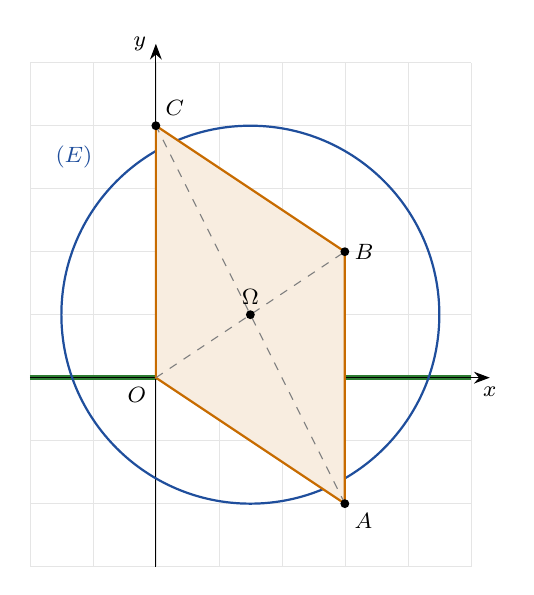
\begin{tikzpicture}[scale=0.8,font=\footnotesize]
\draw[gray!20,very thin] (-2,-3) grid (5,5);
\draw[cRem,line width=1.6pt] (-2,0)--(5,0);
\draw[-{Stealth[length=2mm]}] (-2,0)--(5.3,0) node[below]{$x$};
\draw[-{Stealth[length=2mm]}] (0,-3)--(0,5.3) node[left]{$y$};
\node[below left] at (0,0){$O$};
\begin{scope}\clip (-2,-3) rectangle (5,5);
\draw[cDef,thick] (1.5,1) circle (3);\end{scope}
\node[cDef] at (-1.3,3.5){$(E)$};
\fill[cEx!12] (0,0)--(3,-2)--(3,2)--(0,4)--cycle;
\draw[cEx,thick] (0,0)--(3,-2)--(3,2)--(0,4)--cycle;
\draw[gray,dashed] (0,0)--(3,2) (3,-2)--(0,4);
\fill (3,-2) circle (2pt) node[below right]{$A$};
\fill (3,2) circle (2pt) node[right]{$B$};
\fill (0,4) circle (2pt) node[above right]{$C$};
\fill (1.5,1) circle (2pt) node[above]{$\Omega$};
\end{tikzpicture}\end{LTR}\end{center}
\end{hal}

% ====================== التمرين: 2010 م1 ======================
\begin{tamrin}{بكالوريا 2010 -- الموضوع الأول -- علوم تجريبية}
نعتبر في المستوي المنسوب إلى المعلم المتعامد والمتجانس $(O;\vec u,\vec v)$ النقطتين $A$ و$B$ لاحقتاهما على الترتيب: $z_A=1+i$ و$z_B=3i$.

\textbf{1)} اكتب كلًّا من $z_A$ و$z_B$ على الشكل الأسّي.

\textbf{2)} ليكن $S$ التشابه المباشر الذي يرفق بكلّ نقطة $M$ لاحقتها $z$ النقطة $M'$ لاحقتها $z'$ بحيث: $z'=2iz+6+3i$.
\begin{sq}
\qa عيّن العناصر المميّزة للتشابه المباشر $S$.
\qb عيّن $z_C$ لاحقة النقطة $C$ صورة النقطة $A$ بالتشابه المباشر $S$.
\qc استنتج طبيعة المثلث $ABC$.
\end{sq}
\textbf{3)} لتكن النقطة $D$ مرجح الجملة $\{(A;2),(B;-2),(C;2)\}$.
\begin{sq}
\qa عيّن $z_D$ لاحقة النقطة $D$.
\qb عيّن مع التبرير طبيعة الرباعي $ABCD$.
\end{sq}
\textbf{4)} لتكن $M$ نقطة من المستوي تختلف عن $B$ وعن $D$ لاحقتها $z$، ولتكن $(\Delta)$ مجموعة النقط $M$ ذات اللاحقة $z$ التي يكون من أجلها $\dfrac{z_B-z}{z_D-z}$ عددًا حقيقيًا موجبًا تمامًا.
\begin{sq}
\qa تحقّق أنّ النقطة $E$ ذات اللاحقة $z_E=6+3i$ تنتمي إلى $(\Delta)$.
\qb أعط تفسيرًا هندسيًا لعمدة العدد المركّب $\dfrac{z_B-z}{z_D-z}$. عيّن حينئذ المجموعة $(\Delta)$.
\end{sq}
\end{tamrin}

\begin{hal}
\QQ{1}
$|z_A|=\sqrt2$ و$\cos\theta=\sin\theta=\frac{\sqrt2}{2}$ إذن $\theta=\frac{\pi}{4}$؛ و$z_B=3i=3\left(\cos\frac{\pi}{2}+i\sin\frac{\pi}{2}\right)$:
\[\bx{z_A=\sqrt2\,e^{i\frac{\pi}{4}}}\qquad\bx{z_B=3e^{i\frac{\pi}{2}}}\]
\QQ{2}
\pa $z'=az+b$ مع $a=2i=2e^{i\frac{\pi}{2}}$ و$b=6+3i$: نسبته $|a|=2$ وزاويته $\arg a=\frac{\pi}{2}$. مركزه $\omega$ النقطة الصامدة:
\[\omega=2i\omega+6+3i\iff\omega=\frac{6+3i}{1-2i}=\frac{(6+3i)(1+2i)}{5}=\frac{6+12i+3i+6i^2}{5}=\frac{15i}{5}=3i=z_B .\]
\bxt{$S$ تشابه مباشر مركزه $B$ نسبته $2$ وزاويته $\frac{\pi}{2}$}
\pb $z_C=2i(1+i)+6+3i=2i-2+6+3i$:
\[\bx{z_C=4+5i}\]
\pc $S(A)=C$ ومركز $S$ هو $B$، إذن $z_C-z_B=2i\,(z_A-z_B)$، أي:
\[\frac{z_C-z_B}{z_A-z_B}=\frac{4+2i}{1-2i}=\frac{(4+2i)(1+2i)}{5}=\frac{10i}{5}=2i=2e^{i\frac{\pi}{2}} .\]
ومنه $BC=2BA$ و$(\overrightarrow{BA};\overrightarrow{BC})=\dfrac{\pi}{2}$ بترديد $2\pi$:
\bxt{المثلث $ABC$ قائم في $B$ (و$BC=2BA$)}
\QQ{3}
\pa $2-2+2=2\neq0$، إذن:
\[z_D=\frac{2z_A-2z_B+2z_C}{2}=z_A-z_B+z_C=1+i-3i+4+5i=\bx{5+3i}\]
\pb من $z_D=z_A-z_B+z_C$ نجد $z_B-z_A=z_C-z_D$، أي $\overrightarrow{AB}=\overrightarrow{DC}$، فالرباعي $ABCD$ متوازي أضلاع، وزاويته $\widehat{ABC}$ قائمة (السؤال 2):
\bxt{الرباعي $ABCD$ مستطيل}
(وليس مربّعًا لأنّ $BC=2BA\neq BA$.)
\QQ{4}
\pa $\dfrac{z_B-z_E}{z_D-z_E}=\dfrac{3i-6-3i}{5+3i-6-3i}=\dfrac{-6}{-1}=6$، وهو حقيقي موجب تمامًا:
\bxt{$E\in(\Delta)$}
\pb من أجل $M\neq B$ و$M\neq D$:
\[\arg\left(\frac{z_B-z}{z_D-z}\right)=(\overrightarrow{MD};\overrightarrow{MB})\quad[2\pi].\]
العدد $\dfrac{z_B-z}{z_D-z}$ حقيقي موجب تمامًا إذا وفقط إذا كان $(\overrightarrow{MD};\overrightarrow{MB})=0\ [2\pi]$،
أي الشعاعان $\overrightarrow{MD}$ و$\overrightarrow{MB}$ مرتبطان خطيًا ولهما نفس الاتجاه،
أي $M\in(BD)$ و$M$ خارج القطعة $[BD]$.
\bxt{$(\Delta)$ هو المستقيم $(BD)$ ما عدا القطعة $[BD]$}
بما أنّ $z_B=3i$ و$z_D=5+3i$ فإنّ $(BD)$ هو المستقيم $y=3$، و$(\Delta)$ هي النقط $M(x;3)$ مع $x<0$ أو $x>5$ (وفعلًا $E(6;3)\in(\Delta)$).

\begin{center}\begin{LTR}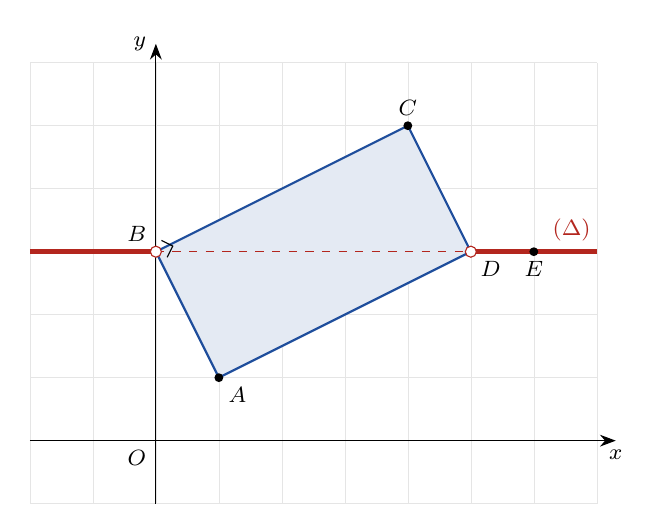
\begin{tikzpicture}[scale=0.8,font=\footnotesize]
\draw[gray!20,very thin] (-2,-1) grid (7,6);
\draw[-{Stealth[length=2mm]}] (-2,0)--(7.3,0) node[below]{$x$};
\draw[-{Stealth[length=2mm]}] (0,-1)--(0,6.3) node[left]{$y$};
\node[below left] at (0,0){$O$};
\fill[cDef!12] (1,1)--(0,3)--(4,5)--(5,3)--cycle;
\draw[cDef,thick] (1,1)--(0,3)--(4,5)--(5,3)--cycle;
\draw (0.179,2.911)--(0.268,3.089)--(0.089,3.179);
\draw[cThm,line width=1.6pt] (-2,3)--(0,3) (5,3)--(7,3);
\draw[cThm,dashed] (0,3)--(5,3);
\draw[cThm,fill=white] (0,3) circle (2.5pt) (5,3) circle (2.5pt);
\node[cThm] at (6.6,3.35){$(\Delta)$};
\fill (1,1) circle (2pt) node[below right]{$A$};
\node[above left] at (0,3){$B$};
\fill (4,5) circle (2pt) node[above]{$C$};
\node[below right] at (5,3){$D$};
\fill (6,3) circle (2pt) node[below]{$E$};
\end{tikzpicture}\end{LTR}\end{center}
\end{hal}

% ====================== التمرين: 2010 م2 ======================
\begin{tamrin}{بكالوريا 2010 -- الموضوع الثاني -- علوم تجريبية}
\textbf{1)} حلّ في مجموعة الأعداد المركّبة $\mathbb{C}$ المعادلة: $z^2-6z+18=0$، ثم اكتب الحلّين على الشكل الأسّي.

\textbf{2)} في المستوي المنسوب إلى المعلم المتعامد والمتجانس $(O;\vec u,\vec v)$ نعتبر النقط $A$، $B$، $C$ و$D$ لواحقها على الترتيب:
\[z_A=3+3i,\qquad z_B=\overline{z_A},\qquad z_C=-z_A,\qquad z_D=-z_B .\]
\begin{sq}
\qa بيّن أنّ النقط $A$، $B$، $C$ و$D$ تنتمي إلى نفس الدائرة ذات المركز $O$.
\qb عيّن زاوية للدوران $R$ الذي مركزه $O$ ويحوّل النقطة $A$ إلى $B$.
\qc بيّن أنّ النقط $A$، $O$ و$C$ في استقامية وكذلك النقط $B$، $O$ و$D$.
\qd استنتج طبيعة الرباعي $ABCD$.
\end{sq}
\end{tamrin}

\begin{hal}
\QQ{1}
$\Delta=36-72=-36=(6i)^2$، إذن $z=\dfrac{6\pm6i}{2}=3\pm3i$.
$|3+3i|=3\sqrt2$ وعمدته $\frac{\pi}{4}$:
\[\bx{3+3i=3\sqrt2\,e^{i\frac{\pi}{4}}}\qquad\bx{3-3i=3\sqrt2\,e^{-i\frac{\pi}{4}}}\]
\QQ{2}
\pa $z_A=3+3i$، $z_B=3-3i$، $z_C=-3-3i$، $z_D=-3+3i$. للأعداد الأربعة نفس الطويلة:
\[OA=OB=OC=OD=\sqrt{9+9}=3\sqrt2 .\]
\bxt{النقط الأربع تنتمي إلى الدائرة التي مركزها $O$ ونصف قطرها $3\sqrt2$}
\pb $z'=e^{i\theta}z$ و$R(A)=B$، إذن:
\[e^{i\theta}=\frac{z_B}{z_A}=\frac{3\sqrt2\,e^{-i\frac{\pi}{4}}}{3\sqrt2\,e^{i\frac{\pi}{4}}}=e^{-i\frac{\pi}{2}}\qquad\Longrightarrow\qquad\bx{\theta=-\frac{\pi}{2}}\]
\pc $z_C=-z_A$ يعني $\dfrac{z_A+z_C}{2}=0=z_O$، أي $O$ منتصف $[AC]$؛ وبالمثل $z_D=-z_B$ يعني $O$ منتصف $[BD]$.
\bxt{$A$ و$O$ و$C$ في استقامية، و$B$ و$O$ و$D$ في استقامية}
\pd قطرا الرباعي $ABCD$ لهما نفس المنتصف $O$ (متوازي أضلاع)، ومتقايسان $AC=BD=6\sqrt2$ (قطران للدائرة) فهو مستطيل، ومتعامدان لأنّ $(\overrightarrow{OA};\overrightarrow{OB})=-\frac{\pi}{2}$ فهو معيّن:
\bxt{الرباعي $ABCD$ مربّع}

\begin{center}\begin{LTR}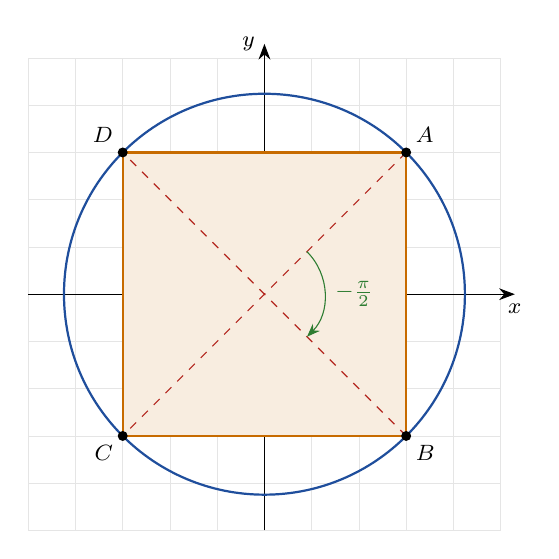
\begin{tikzpicture}[scale=0.6,font=\footnotesize]
\draw[gray!20,very thin] (-5,-5) grid (5,5);
\draw[-{Stealth[length=2mm]}] (-5,0)--(5.3,0) node[below]{$x$};
\draw[-{Stealth[length=2mm]}] (0,-5)--(0,5.3) node[left]{$y$};
\node[below left] at (0,0){$O$};
\draw[cDef,thick] (0,0) circle (4.243);
\fill[cEx!12] (3,3)--(3,-3)--(-3,-3)--(-3,3)--cycle;
\draw[cEx,thick] (3,3)--(3,-3)--(-3,-3)--(-3,3)--cycle;
\draw[cThm,dashed] (3,3)--(-3,-3) (3,-3)--(-3,3);
\draw[cRem,-{Stealth}] (0.9,0.9) arc (45:-45:1.273);
\node[cRem] at (1.9,0){$-\frac{\pi}{2}$};
\fill (3,3) circle (3pt) node[above right]{$A$};
\fill (3,-3) circle (3pt) node[below right]{$B$};
\fill (-3,-3) circle (3pt) node[below left]{$C$};
\fill (-3,3) circle (3pt) node[above left]{$D$};
\end{tikzpicture}\end{LTR}\end{center}
\end{hal}

% ====================== التمرين: 2009 م1 ======================
\begin{tamrin}{بكالوريا 2009 -- الموضوع الأول -- علوم تجريبية}
$P(z)$ كثير حدود حيث: $P(z)=(z-1-i)(z^2-2z+4)$ و$z$ عدد مركّب.

\textbf{1)} حلّ في المجموعة $\mathbb{C}$ المعادلة: $P(z)=0$.

\textbf{2)} نضع: $z_1=1+i$، $z_2=1-i\sqrt3$.
\begin{sq}
\qa اكتب $z_1$ و$z_2$ على الشكل الأسّي.
\qb اكتب $\dfrac{z_1}{z_2}$ على الشكل الجبري ثم الشكل الأسّي.
\qc استنتج القيمة المضبوطة لكلّ من $\sin\left(\dfrac{7\pi}{12}\right)$ و$\cos\left(\dfrac{7\pi}{12}\right)$.
\end{sq}
\textbf{3)}
\begin{sq}
\qa $n$ عدد طبيعي، عيّن قيم $n$ بحيث يكون العدد $\left(\dfrac{z_1}{z_2}\right)^{n}$ حقيقيًا.
\qb احسب قيمة العدد $\left(\dfrac{z_1}{z_2}\right)^{456}$.
\end{sq}
\end{tamrin}

\begin{hal}
\QQ{1}
$P(z)=0\iff z-1-i=0$ أو $z^2-2z+4=0$.
\begin{itemize}
\item $z-1-i=0\iff z=1+i$.
\item $z^2-2z+4=0$: $\Delta=4-16=-12=\left(2i\sqrt3\right)^2$، إذن $z=\dfrac{2\pm2i\sqrt3}{2}=1\pm i\sqrt3$.
\end{itemize}
\[\bx{S=\left\{1+i\,;\,1-i\sqrt3\,;\,1+i\sqrt3\right\}}\]
\QQ{2}
\pa $|z_1|=\sqrt2$ وعمدته $\frac{\pi}{4}$. $|z_2|=\sqrt{1+3}=2$، $\cos\theta=\frac12$، $\sin\theta=-\frac{\sqrt3}{2}$ إذن $\theta=-\frac{\pi}{3}$:
\[\bx{z_1=\sqrt2\,e^{i\frac{\pi}{4}}}\qquad\bx{z_2=2e^{-i\frac{\pi}{3}}}\]
\pb \textbf{الشكل الجبري:}
\[\frac{z_1}{z_2}=\frac{(1+i)(1+i\sqrt3)}{(1-i\sqrt3)(1+i\sqrt3)}=\frac{1+i\sqrt3+i+i^2\sqrt3}{4}=\bx{\frac{1-\sqrt3}{4}+i\,\frac{1+\sqrt3}{4}}\]
\textbf{الشكل الأسّي:}
\[\frac{z_1}{z_2}=\frac{\sqrt2}{2}\,e^{i\left(\frac{\pi}{4}+\frac{\pi}{3}\right)}=\bx{\frac{\sqrt2}{2}\,e^{i\frac{7\pi}{12}}}\]
\pc بالمطابقة: $\dfrac{\sqrt2}{2}\cos\dfrac{7\pi}{12}=\dfrac{1-\sqrt3}{4}$ و$\dfrac{\sqrt2}{2}\sin\dfrac{7\pi}{12}=\dfrac{1+\sqrt3}{4}$، ومنه:
\[\cos\frac{7\pi}{12}=\frac{1-\sqrt3}{2\sqrt2}=\bx{\frac{\sqrt2-\sqrt6}{4}}\qquad \sin\frac{7\pi}{12}=\frac{1+\sqrt3}{2\sqrt2}=\bx{\frac{\sqrt2+\sqrt6}{4}}\]
\QQ{3}
\pa $\left(\dfrac{z_1}{z_2}\right)^n=\left(\dfrac{\sqrt2}{2}\right)^n e^{i\frac{7n\pi}{12}}$، وطويلته غير معدومة. يكون حقيقيًا إذا وفقط إذا كانت عمدته من الشكل $k\pi$:
\[\frac{7n\pi}{12}=k\pi\ (k\in\Z)\iff 7n=12k .\]
إذن $12$ يقسم $7n$، وبما أنّ $7$ و$12$ أوّليان فيما بينهما فإنّ $12$ يقسم $n$:
\[\bx{n=12k,\ k\in\N}\]
\pb $456=12\times38$ فالعدد حقيقي:
\[\left(\frac{z_1}{z_2}\right)^{456}=\left(\frac{\sqrt2}{2}\right)^{456}e^{i\frac{7\times456\,\pi}{12}}=\left(\frac{1}{2}\right)^{228}e^{i\,266\pi}=\frac{1}{2^{228}}\times1\]
لأنّ $\left(\frac{\sqrt2}{2}\right)^2=\frac12$ و$266\pi=133\times2\pi$:
\[\bx{\left(\frac{z_1}{z_2}\right)^{456}=\frac{1}{2^{228}}}\]
\end{hal}

% ====================== التمرين: 2009 م2 ======================
\begin{tamrin}{بكالوريا 2009 -- الموضوع الثاني -- علوم تجريبية}
المستوي منسوب إلى المعلم المتعامد والمتجانس $(O;\vec i,\vec j)$.

\textbf{1)} حلّ في المجموعة $\mathbb{C}$ المعادلة: $z^2-2z+4=0$.

\textbf{2)} نسمّي $z_1$ و$z_2$ حلّي هذه المعادلة.
\begin{sq}
\qa اكتب العددين $z_1$ و$z_2$ على الشكل الأسّي.
\qb $A$، $B$ و$C$ هي النقط من المستوي التي لواحقها على الترتيب: $z_A=1-i\sqrt3$، $z_B=1+i\sqrt3$ و$z_C=\dfrac12\left(5+i\sqrt3\right)$.
احسب الأطوال $AB$، $AC$ و$BC$، ثم استنتج طبيعة المثلث $ABC$.
\qc جد الطويلة وعمدة للعدد المركّب $z$ حيث: $z=\dfrac{z_C-z_B}{z_A-z_B}$.
\qd احسب $z^3$، $z^6$ ثم استنتج أنّ $z^{3k}$ عدد حقيقي من أجل كلّ عدد طبيعي $k$.
\end{sq}
\end{tamrin}

\begin{hal}
\QQ{1}
$\Delta=4-16=-12=\left(2i\sqrt3\right)^2$، إذن:
\[\bx{S=\left\{1-i\sqrt3\,;\,1+i\sqrt3\right\}}\]
\QQ{2}
\pa نضع $z_1=1-i\sqrt3$ و$z_2=1+i\sqrt3=\overline{z_1}$. الطويلة $\sqrt{1+3}=2$، و$\cos\theta=\frac12$، $\sin\theta=-\frac{\sqrt3}{2}$ إذن $\theta=-\frac{\pi}{3}$:
\[\bx{z_1=2e^{-i\frac{\pi}{3}}}\qquad\bx{z_2=2e^{i\frac{\pi}{3}}}\]
\pb
\begin{align*}
AB&=|z_B-z_A|=\left|2i\sqrt3\right|=2\sqrt3,\\
AC&=|z_C-z_A|=\left|\tfrac32+\tfrac{3\sqrt3}{2}i\right|=\sqrt{\tfrac94+\tfrac{27}{4}}=\sqrt9=3,\\
BC&=|z_C-z_B|=\left|\tfrac32-\tfrac{\sqrt3}{2}i\right|=\sqrt{\tfrac94+\tfrac34}=\sqrt3 .
\end{align*}
$AC^2+BC^2=9+3=12=AB^2$، فحسب عكس مبرهنة فيثاغورس:
\bxt{المثلث $ABC$ قائم في $C$}
\pc
\[z=\frac{z_C-z_B}{z_A-z_B}=\frac{\frac32-\frac{\sqrt3}{2}i}{-2i\sqrt3}=\frac{3-i\sqrt3}{-4i\sqrt3}=\frac{(3-i\sqrt3)\,i}{-4i^2\sqrt3}=\frac{\sqrt3+3i}{4\sqrt3}=\frac14+\frac{\sqrt3}{4}i .\]
$|z|=\sqrt{\frac{1}{16}+\frac{3}{16}}=\frac12$ (وهو $\frac{BC}{BA}=\frac{\sqrt3}{2\sqrt3}$)، و$\cos\theta=\frac{1/4}{1/2}=\frac12$، $\sin\theta=\frac{\sqrt3}{2}$:
\[\bx{|z|=\frac12}\qquad\bx{\arg z=\frac{\pi}{3}\ [2\pi]}\qquad\left(z=\tfrac12 e^{i\frac{\pi}{3}}\right)\]
\pd $z^3=\left(\frac12\right)^3e^{i\pi}=\bx{-\dfrac18}$ و$z^6=\left(z^3\right)^2=\bx{\dfrac{1}{64}}$.
من أجل كلّ $k\in\N$: $z^{3k}=\left(z^3\right)^k=\left(-\dfrac18\right)^k$ وهو عدد حقيقي:
\bxt{$z^{3k}$ عدد حقيقي من أجل كلّ عدد طبيعي $k$}

\begin{center}\begin{LTR}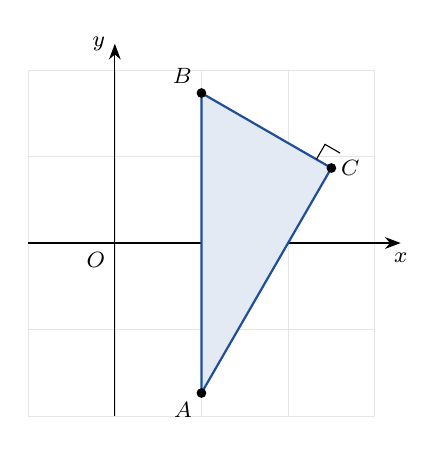
\begin{tikzpicture}[scale=1.1,font=\footnotesize]
\draw[gray!20,very thin] (-1,-2) grid (3,2);
\draw[-{Stealth[length=2mm]}] (-1,0)--(3.3,0) node[below]{$x$};
\draw[-{Stealth[length=2mm]}] (0,-2)--(0,2.3) node[left]{$y$};
\node[below left] at (0,0){$O$};
\fill[cDef!12] (1,-1.732)--(1,1.732)--(2.5,0.866)--cycle;
\draw[cDef,thick] (1,-1.732)--(1,1.732)--(2.5,0.866)--cycle;
\draw (2.5,0.866) ++(-0.173,0.1) -- ++(0.1,0.173) -- ++(0.173,-0.1);
\fill (1,-1.732) circle (1.6pt) node[below left]{$A$};
\fill (1,1.732) circle (1.6pt) node[above left]{$B$};
\fill (2.5,0.866) circle (1.6pt) node[right]{$C$};
\end{tikzpicture}\end{LTR}\end{center}
\end{hal}

% ====================== التمرين: 2008 م1 ======================
\begin{tamrin}{بكالوريا 2008 -- الموضوع الأول -- علوم تجريبية}
\textbf{1)} حلّ في مجموعة الأعداد المركّبة $\mathbb{C}$ المعادلة: $z^2-(1+2i)z-1+i=0$.
نرمز للحلّين بـ $z_1$ و$z_2$ حيث $|z_1|<|z_2|$. بيّن أنّ $\left(\dfrac{z_1}{z_2}\right)^{2008}$ عدد حقيقي.

\textbf{2)} المستوي المركّب منسوب إلى المعلم المتعامد والمتجانس $(O;\vec u,\vec v)$.
لتكن $A$، $B$ و$C$ نقطًا من المستوي لواحقها على الترتيب: $1$، $z_1$ و$z_2$. ليكن $z$ العدد المركّب حيث: $z=\dfrac{z_2-1}{z_1-1}$.
\begin{sq}
\qa انطلاقًا من التعريف $e^{i\theta}=\cos\theta+i\sin\theta$ ومن الخاصية $e^{i(\theta_1+\theta_2)}=e^{i\theta_1}\times e^{i\theta_2}$،
برهن أنّ: $e^{-i\theta}=\dfrac{1}{e^{i\theta}}$ وأنّ: $\dfrac{e^{i\theta_1}}{e^{i\theta_2}}=e^{i(\theta_1-\theta_2)}$ حيث $\theta$، $\theta_1$ و$\theta_2$ أعداد حقيقية.
\qb اكتب $z$ على الشكل الأسّي.
\qc اكتب $z$ على الشكل المثلثي واستنتج أنّ $C$ هي صورة $B$ بتشابه مباشر مركزه $A$، يُطلب تعيين نسبته وزاويته.
\end{sq}
\end{tamrin}

\begin{molahada}
في نصّ المصدر كُتبت المساواة المطلوب برهانها على الشكل $\dfrac{e^{i\theta_1}}{e^{i\theta_2}}=e^{i(\theta_1+\theta_2)}$ وهي خاطئة (مثلًا من أجل $\theta_1=\theta_2=\frac{\pi}{2}$ يكون الطرف الأيسر $1$ والأيمن $-1$)؛ صُحّحت إلى $e^{i(\theta_1-\theta_2)}$.
\end{molahada}

\begin{hal}
\QQ{1}
$\Delta=(1+2i)^2-4(-1+i)=1+4i-4+4-4i=1=1^2$، إذن:
\[z=\frac{1+2i-1}{2}=i\qquad;\qquad z=\frac{1+2i+1}{2}=1+i .\]
$|i|=1<|1+i|=\sqrt2$، إذن $\bx{z_1=i}$ و$\bx{z_2=1+i}$.
\[\frac{z_1}{z_2}=\frac{i(1-i)}{(1+i)(1-i)}=\frac{1+i}{2}=\frac{\sqrt2}{2}\,e^{i\frac{\pi}{4}}\]
\[\left(\frac{z_1}{z_2}\right)^{2008}=\left(\frac{\sqrt2}{2}\right)^{2008}e^{i\frac{2008\pi}{4}}=\left(\frac12\right)^{1004}e^{i\,502\pi}=\bx{\frac{1}{2^{1004}}}\in\R\]
لأنّ $502\pi=251\times2\pi$.
\QQ{2}
\pa من الخاصية:
\[e^{i\theta}\times e^{-i\theta}=e^{i(\theta-\theta)}=e^{i0}=\cos0+i\sin0=1 ,\]
و$e^{i\theta}\neq0$ لأنّ $|e^{i\theta}|=\sqrt{\cos^2\theta+\sin^2\theta}=1$، إذن:
\[\bx{e^{-i\theta}=\frac{1}{e^{i\theta}}}\]
ثم: $\dfrac{e^{i\theta_1}}{e^{i\theta_2}}=e^{i\theta_1}\times\dfrac{1}{e^{i\theta_2}}=e^{i\theta_1}\times e^{-i\theta_2}=e^{i(\theta_1+(-\theta_2))}$:
\[\bx{\frac{e^{i\theta_1}}{e^{i\theta_2}}=e^{i(\theta_1-\theta_2)}}\]
\pb $z=\dfrac{z_2-1}{z_1-1}=\dfrac{i}{-1+i}$، مع $i=e^{i\frac{\pi}{2}}$ و$-1+i=\sqrt2\,e^{i\frac{3\pi}{4}}$، ومن (أ):
\[z=\frac{1}{\sqrt2}\,e^{i\left(\frac{\pi}{2}-\frac{3\pi}{4}\right)}=\bx{\frac{\sqrt2}{2}\,e^{-i\frac{\pi}{4}}}\]
(تحقّق جبريًا: $z=\frac{i(-1-i)}{(-1+i)(-1-i)}=\frac{1-i}{2}$.)
\pc \[z=\frac{\sqrt2}{2}\left(\cos\left(-\frac{\pi}{4}\right)+i\sin\left(-\frac{\pi}{4}\right)\right).\]
بما أنّ $z_A=1$ فإنّ $z=\dfrac{z_C-z_A}{z_B-z_A}$، إذن:
\[z_C-z_A=\frac{\sqrt2}{2}e^{-i\frac{\pi}{4}}(z_B-z_A)\]
\bxt{$C$ صورة $B$ بالتشابه المباشر الذي مركزه $A$ ونسبته $\frac{\sqrt2}{2}$ وزاويته $-\frac{\pi}{4}$}

\begin{center}\begin{LTR}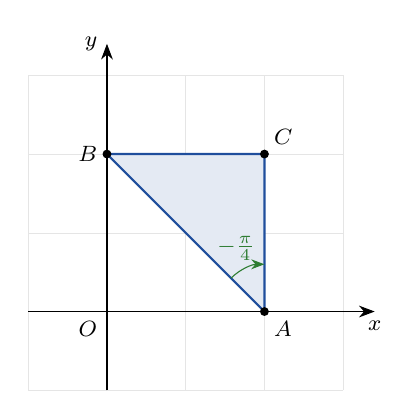
\begin{tikzpicture}[scale=2,font=\footnotesize]
\draw[gray!20,very thin] (-0.5,-0.5) grid[step=0.5] (1.5,1.5);
\draw[-{Stealth[length=2mm]}] (-0.5,0)--(1.7,0) node[below]{$x$};
\draw[-{Stealth[length=2mm]}] (0,-0.5)--(0,1.7) node[left]{$y$};
\node[below left] at (0,0){$O$};
\fill[cDef!12] (1,0)--(0,1)--(1,1)--cycle;
\draw[cDef,thick] (1,0)--(0,1)--(1,1)--cycle;
\draw[cRem,-{Stealth}] ($(1,0)+(135:0.3)$) arc (135:90:0.3);
\node[cRem] at (0.82,0.4){$-\frac{\pi}{4}$};
\fill (1,0) circle (0.8pt) node[below right]{$A$};
\fill (0,1) circle (0.8pt) node[left]{$B$};
\fill (1,1) circle (0.8pt) node[above right]{$C$};
\end{tikzpicture}\end{LTR}\end{center}
\end{hal}

% ====================== التمرين: 2008 م2 ======================
\begin{tamrin}{بكالوريا 2008 -- الموضوع الثاني -- علوم تجريبية}
\textbf{1)} حلّ في مجموعة الأعداد المركّبة $\mathbb{C}$ المعادلة ذات المجهول $z$ التالية: $z^2+iz-2-6i=0$.

\textbf{2)} نعتبر في المستوي المركّب المنسوب إلى المعلم المتعامد والمتجانس $(O;\vec u,\vec v)$ النقطتين $A$ و$B$ اللتين لاحقتاهما $z_A$ و$z_B$ على الترتيب حيث: $z_A=2+i$ و$z_B=-2-2i$.
عيّن $z_\omega$ لاحقة النقطة $\omega$ مركز الدائرة $(\Gamma)$ ذات القطر $[AB]$.

\textbf{3)} لتكن $C$ النقطة ذات اللاحقة $z_C$ حيث: $z_C=\dfrac{4-i}{1+i}$.
اكتب $z_C$ على الشكل الجبري ثم أثبت أنّ النقطة $C$ تنتمي إلى الدائرة $(\Gamma)$.

\textbf{4)}
\begin{sq}
\qa برهن أنّ عبارة التشابه المباشر الذي مركزه $M_0(z_0)$ ونسبته $k$ ($k>0$) وزاويته $\theta$ والذي يرفق بكلّ نقطة $M(z)$ النقطة $M'(z')$ هي: $z'-z_0=ke^{i\theta}(z-z_0)$.
\qb \textbf{تطبيق:} عيّن الطبيعة والعناصر المميّزة للتحويل $S$ المعرّف بـ: $z'+\dfrac12 i=2e^{i\frac{\pi}{3}}\left(z+\dfrac12 i\right)$.
\end{sq}
\end{tamrin}

\begin{hal}
\QQ{1}
المعاملات مركّبة: $\Delta=i^2-4(-2-6i)=-1+8+24i=7+24i$.
نبحث عن $\delta=x+iy$ ($x,y\in\R$) حيث $\delta^2=\Delta$: $x^2-y^2=7$، $2xy=24$، و$x^2+y^2=|\Delta|=\sqrt{49+576}=25$.
بالجمع: $2x^2=32$ أي $x^2=16$، وبالطرح: $y^2=9$، و$xy=12>0$ إذن $\delta=4+3i$ (تحقّق: $(4+3i)^2=16+24i-9=7+24i$).
\[z=\frac{-i+(4+3i)}{2}=2+i\qquad;\qquad z=\frac{-i-(4+3i)}{2}=-2-2i .\]
\[\bx{S=\{2+i\,;\,-2-2i\}}\]
\QQ{2}
مركز الدائرة ذات القطر $[AB]$ هو منتصف $[AB]$:
\[z_\omega=\frac{z_A+z_B}{2}=\frac{2+i-2-2i}{2}=\bx{-\frac12 i}\]
ونصف قطرها $r=\dfrac{AB}{2}=\dfrac{|-4-3i|}{2}=\dfrac52$.
\QQ{3}
\[z_C=\frac{(4-i)(1-i)}{(1+i)(1-i)}=\frac{4-4i-i+i^2}{2}=\bx{\frac32-\frac52 i}\]
\[\omega C=\left|z_C-z_\omega\right|=\left|\frac32-\frac52 i+\frac12 i\right|=\left|\frac32-2i\right|=\sqrt{\frac94+4}=\sqrt{\frac{25}{4}}=\frac52=r .\]
\bxt{النقطة $C$ تنتمي إلى الدائرة $(\Gamma)$}
\QQ{4}
\pa التشابه المباشر $S$ الذي مركزه $M_0$ ونسبته $k>0$ وزاويته $\theta$ معرّف بـ:
\begin{itemize}
\item $S(M_0)=M_0$؛
\item من أجل $M\neq M_0$: $M'=S(M)$ يعني $M_0M'=k\,M_0M$ و$(\overrightarrow{M_0M};\overrightarrow{M_0M'})=\theta\ [2\pi]$.
\end{itemize}
بالأعداد المركّبة، من أجل $z\neq z_0$:
\[\left|\frac{z'-z_0}{z-z_0}\right|=\frac{M_0M'}{M_0M}=k ,\]
\[\arg\left(\frac{z'-z_0}{z-z_0}\right)=(\overrightarrow{M_0M};\overrightarrow{M_0M'})=\theta\ [2\pi],\]
إذن $\dfrac{z'-z_0}{z-z_0}=ke^{i\theta}$، أي $z'-z_0=ke^{i\theta}(z-z_0)$. ومن أجل $M=M_0$: $z'=z_0$ تحقّق العلاقة أيضًا ($0=0$):
\[\bx{z'-z_0=ke^{i\theta}(z-z_0)}\]
\pb $z'+\frac12 i=2e^{i\frac{\pi}{3}}\left(z+\frac12 i\right)\iff z'-\left(-\frac12 i\right)=2e^{i\frac{\pi}{3}}\left(z-\left(-\frac12 i\right)\right)$، وهي من الشكل السابق مع $z_0=-\frac12 i=z_\omega$، $k=2$، $\theta=\frac{\pi}{3}$:
\bxt{$S$ تشابه مباشر مركزه $\omega$ (مركز $(\Gamma)$) نسبته $2$ وزاويته $\frac{\pi}{3}$}

\begin{center}\begin{LTR}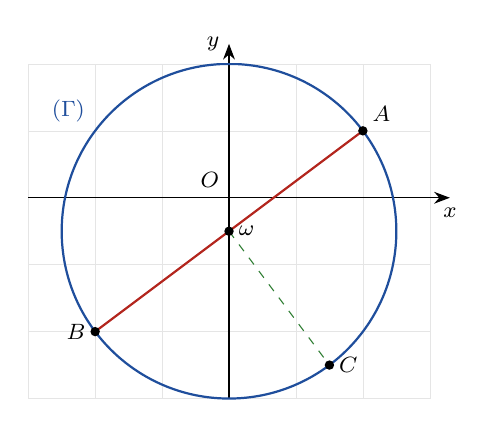
\begin{tikzpicture}[scale=0.85,font=\footnotesize]
\draw[gray!20,very thin] (-3,-3) grid (3,2);
\draw[-{Stealth[length=2mm]}] (-3,0)--(3.3,0) node[below]{$x$};
\draw[-{Stealth[length=2mm]}] (0,-3)--(0,2.3) node[left]{$y$};
\node[above left] at (0,0){$O$};
\begin{scope}\clip (-3,-3.2) rectangle (3,2);
\draw[cDef,thick] (0,-0.5) circle (2.5);\end{scope}
\node[cDef] at (-2.4,1.3){$(\Gamma)$};
\draw[cThm,thick] (2,1)--(-2,-2);
\draw[cRem,dashed] (0,-0.5)--(1.5,-2.5);
\fill (2,1) circle (2pt) node[above right]{$A$};
\fill (-2,-2) circle (2pt) node[left]{$B$};
\fill (0,-0.5) circle (2pt) node[right]{$\omega$};
\fill (1.5,-2.5) circle (2pt) node[right]{$C$};
\end{tikzpicture}\end{LTR}\end{center}
\end{hal}
\section{تمارين البكالوريا -- شعبة تقني رياضي}
% ---------- helpers for the figures of this part (complex plane) ----------
% \begin{cpoCP}{u}{v}{xmin}{xmax}{ymin}{ymax}{unit cm} ... \end{cpoCP}
\newenvironment{cpoCP}[7]{\par\begin{center}\begin{LTR}\begin{tikzpicture}[x=#7cm,y=#7cm,font=\footnotesize,line cap=round]
 \draw[gray!20,very thin] (#3,#5) grid (#4,#6);
 \draw[-{Stealth[length=2mm]},gray!80!black] (#3,0)--(#4,0);
 \draw[-{Stealth[length=2mm]},gray!80!black] (0,#5)--(0,#6);
 \draw[very thick,-{Stealth[length=1.8mm]},black] (0,0)--(1,0) node[below,pos=0.55]{$\vec{#1}$};
 \draw[very thick,-{Stealth[length=1.8mm]},black] (0,0)--(0,1) node[left,pos=0.55]{$\vec{#2}$};
 \node[below left,inner sep=1.5pt] at (0,0){$O$};}
{\end{tikzpicture}\end{LTR}\end{center}}
% filled point with label: \cpoD{coord}{anchor}{label}
\newcommand{\cpoD}[3]{\fill (#1) circle (1.7pt) node[#2]{$#3$};}
% right-angle mark at #1 between directions #2 and #3
\newcommand{\cpoRA}[3]{\draw[thin] ($(#1)!2.6mm!(#2)$) -- ($($(#1)!2.6mm!(#2)$)+($(#1)!2.6mm!(#3)$)-(#1)$) -- ($(#1)!2.6mm!(#3)$);}
% equal-length tick on segment [#1#2]
\newcommand{\cpoT}[2]{\path ($(#1)!0.5!(#2)$) coordinate (cpoM); \draw[thick] ($(cpoM)!1.5mm!90:(#2)$) -- ($(cpoM)!1.5mm!-90:(#2)$);}
\newcommand{\cpoTT}[2]{\path ($(#1)!0.5!(#2)$) coordinate (cpoM); \draw[thick] ($($(cpoM)!1.5mm!90:(#2)$)!0.6mm!(#2)$) -- ($($(cpoM)!1.5mm!-90:(#2)$)!0.6mm!(#2)$); \draw[thick] ($($(cpoM)!1.5mm!90:(#2)$)!-0.6mm!(#2)$) -- ($($(cpoM)!1.5mm!-90:(#2)$)!-0.6mm!(#2)$);}

% ===================== 2019 - S1 - TM =====================
\begin{tamrin}{بكالوريا 2019 -- الموضوع الأول -- تقني رياضي}
المستوي المركب منسوب إلى المعلم المتعامد والمتجانس $(O;\vec u,\vec v)$. $A$، $B$ و $C$ النقط التي لواحقها على الترتيب:
\[z_A=1+i,\qquad z_B=2+i,\qquad z_C=\frac32+i\left(1+\frac{\sqrt3}{2}\right).\]
$(\Gamma)$ الدائرة التي مركزها $A$ ونصف قطرها $1$.

\QQ{1}
\begin{sq}
\qa تحقق أن النقطة $C$ من الدائرة $(\Gamma)$.
\qb عين قيسا بالراديان للزاوية $\left(\overrightarrow{AB};\overrightarrow{AC}\right)$، ثم استنتج أن $C$ صورة $B$ بالدوران $r$ الذي مركزه $A$ يطلب تعيين زاويته.
\end{sq}
\QQ{2} $S$ التشابه المباشر الذي يحول النقطة $M$ ذات اللاحقة $z$ إلى النقطة $M'$ ذات اللاحقة $z'$ حيث: $z'=(1+i\sqrt3)z+\sqrt3-i\sqrt3$.
\begin{sq}
\qa حدد العناصر المميزة للتشابه $S$.
\qb عين $z_D$ لاحقة $D$ صورة $B$ بالتشابه $S$.
\end{sq}
\QQ{3} ما هي نسبة التحاكي $h$ الذي مركزه $A$ حيث: $S=h\circ r$؟ استنتج أن النقط $A$، $C$ و $D$ في استقامية.

\QQ{4} $(E)$ مجموعة النقط $M$ من المستوي ذات اللاحقة $z$ حيث: $z=z_A+k\,e^{i\frac{\pi}{3}}$ مع $k\in\mathbb{R}_+^*$.
تحقق أن النقطة $C$ تنتمي إلى $(E)$، ثم حدد طبيعة المجموعة $(E)$.
\end{tamrin}

\begin{hal}
\QQ{1}
\pa $z_C-z_A=\frac12+i\frac{\sqrt3}{2}$، ومنه $AC=|z_C-z_A|=\sqrt{\frac14+\frac34}=1$. إذن $AC=1$ أي \bxt{$C\in(\Gamma)$}.

\pb $z_B-z_A=1$ و $z_C-z_A=\frac12+i\frac{\sqrt3}{2}=e^{i\frac{\pi}{3}}$، ومنه:
\[\left(\overrightarrow{AB};\overrightarrow{AC}\right)=\arg\frac{z_C-z_A}{z_B-z_A}=\arg e^{i\frac{\pi}{3}}\qquad\Longrightarrow\qquad\bx{\left(\overrightarrow{AB};\overrightarrow{AC}\right)=\frac{\pi}{3}\ [2\pi]}\]
وبما أن $AB=|1|=1=AC$ فإن $z_C-z_A=e^{i\frac{\pi}{3}}(z_B-z_A)$: \bxt{$C$ صورة $B$ بالدوران $r$ الذي مركزه $A$ وزاويته $\frac{\pi}{3}$}.

\QQ{2}
\pa $z'=az+b$ مع $a=1+i\sqrt3$ و $b=\sqrt3-i\sqrt3$. $a=2\left(\frac12+i\frac{\sqrt3}{2}\right)=2e^{i\frac{\pi}{3}}$:
\begin{itemize}
\item النسبة $|a|=2$، والزاوية $\arg a=\frac{\pi}{3}$.
\item المركز $\omega$: $z_\omega=\dfrac{b}{1-a}=\dfrac{\sqrt3(1-i)}{-i\sqrt3}=\dfrac{1-i}{-i}=(1-i)\,i=1+i=z_A$.
\end{itemize}
\bxt{$S$ تشابه مباشر مركزه $A$، نسبته $2$ وزاويته $\frac{\pi}{3}$}.

\pb $z_D=(1+i\sqrt3)(2+i)+\sqrt3-i\sqrt3=2+i+2i\sqrt3-\sqrt3+\sqrt3-i\sqrt3$، إذن \bx{z_D=2+i(1+\sqrt3)}.

\QQ{3} $r$ الدوران الذي مركزه $A$ وزاويته $\frac{\pi}{3}$، و $h$ تحاك مركزه $A$ ونسبته $\lambda$. كتابتهما: $r$: $z_1-z_A=e^{i\frac{\pi}{3}}(z-z_A)$، $h$: $z'-z_A=\lambda(z_1-z_A)$، إذن:
\[h\circ r:\ z'-z_A=\lambda e^{i\frac{\pi}{3}}(z-z_A)\]
وكتابة $S$: $z'-z_A=2e^{i\frac{\pi}{3}}(z-z_A)$. بالمطابقة: \bx{\lambda=2}.

$D=S(B)=h\big(r(B)\big)=h(C)$، إذن $\overrightarrow{AD}=2\overrightarrow{AC}$، ومنه \bxt{النقط $A$، $C$ و $D$ في استقامية}.
(تحقق: $z_D-z_A=1+i\sqrt3=2\left(\frac12+i\frac{\sqrt3}{2}\right)=2(z_C-z_A)$.)

\QQ{4} من أجل $k=1$: $z=z_A+e^{i\frac{\pi}{3}}=1+i+\frac12+i\frac{\sqrt3}{2}=z_C$، إذن \bxt{$C\in(E)$}.

لدينا $z-z_A=k\,e^{i\frac{\pi}{3}}=k(z_C-z_A)$. إذن $\overrightarrow{AM}=k\,\overrightarrow{AC}$ حيث $k$ يمسح $]0;+\infty[$، ومنه:

\bxt{$(E)$ نصف المستقيم $[AC)$ الذي مبدؤه $A$ ويشمل $C$، باستثناء النقطة $A$}.
\begin{cpoCP}{u}{v}{-0.6}{3}{-0.6}{3.4}{1.4}
 \coordinate (A) at (1,1); \coordinate (B) at (2,1); \coordinate (C) at (1.5,1.866); \coordinate (D) at (2,2.732);
 \draw[cDef,thick] (A) circle (1);
 \draw[cThm,very thick,-{Stealth[length=2.5mm]}] (A)--(2.35,3.34);
 \draw[cEx,thick] (A)--(B)--(C)--cycle;
 \draw[cRem,thick,-{Stealth[length=2mm]}] (1.45,1) arc (0:60:0.45);
 \node[cRem] at (1.62,1.3){$\frac{\pi}{3}$};
 \fill[white] (A) circle (2.2pt); \draw[cThm] (A) circle (2.2pt); \node[left] at (A){$A$};
 \cpoD{B}{right}{B} \cpoD{C}{right}{C} \cpoD{D}{right}{D}
 \node[cDef] at (0.2,0.2){$(\Gamma)$}; \node[cThm] at (2.6,3.2){$(E)$};
\end{cpoCP}
\end{hal}

% ===================== 2019 - S2 - TM =====================
\begin{tamrin}{بكالوريا 2019 -- الموضوع الثاني -- تقني رياضي}
\textbf{I)} تحقق أن: $(2-2\sqrt3)^2=16-8\sqrt3$.
\textbf{II)} المستوي المركب منسوب إلى المعلم المتعامد والمتجانس $(O;\vec u,\vec v)$. نعتبر النقط $A$، $B$ و $C$ التي لواحقها على الترتيب:
\[z_A=4e^{i\frac{\pi}{3}}+4e^{i\frac{5\pi}{6}},\qquad z_B=\frac12iz_A,\qquad z_C=-\frac14z_A.\]
\QQ{1} أكتب $z_A$ على الشكل الجبري، ثم بين أن: $z_A=4\sqrt2\,e^{i\frac{7\pi}{12}}$.

\QQ{2} استنتج القيمتين المضبوطتين للعددين الحقيقيين $\cos\left(\dfrac{7\pi}{12}\right)$ و $\sin\left(\dfrac{7\pi}{12}\right)$.

\QQ{3} $S$ التشابه المباشر الذي يحول $A$ إلى $B$ و $B$ إلى $C$. لتكن $M'$ النقطة ذات اللاحقة $z'$ صورة النقطة $M$ ذات اللاحقة $z$ بالتشابه $S$.
\begin{sq}
\qa بين أن: $z'=\dfrac12iz$.
\qb حدد العناصر المميزة للتشابه $S$.
\end{sq}
\QQ{4} $G$ النقطة ذات اللاحقة $z_G$ مرجح الجملة $\{(A;2),(B;-2),(C;4)\}$.
\begin{sq}
\qa بين أن: $z_G=2e^{i\frac{\pi}{3}}$.
\qb $(E)$ مجموعة النقط $M$ من المستوي ذات اللاحقة $z$ حيث: $\left\|\overrightarrow{MA}-\overrightarrow{MB}+2\overrightarrow{MC}\right\|=2\sqrt2$.
حدد طبيعة المجموعة $(E)$ وعناصرها المميزة، ثم أحسب محيط $(E')$ صورة $(E)$ بالتشابه $S$.
\end{sq}
\begin{molahada}
حُذف السؤال I(ب) «أكتب على الشكل الجبري الجذرين التربيعيين $L_1$ و$L_2$ للعدد المركب $z=-16\sqrt3-16i$» لأنه خارج المنهاج الحالي (التوزيع السنوي 2026-2027): الجذران التربيعيان لعدد مركب مقرران في شعبة علوم تجريبية فقط.
\end{molahada}
\end{tamrin}

\begin{hal}
\textbf{الجزء I:}
$(2-2\sqrt3)^2=4-8\sqrt3+12=16-8\sqrt3$. \ok

\textbf{الجزء II:}
\QQ{1} $4e^{i\frac{\pi}{3}}=2+2i\sqrt3$ و $4e^{i\frac{5\pi}{6}}=4\left(-\frac{\sqrt3}{2}+\frac12i\right)=-2\sqrt3+2i$، إذن:
\[\bx{z_A=(2-2\sqrt3)+i(2+2\sqrt3)}\]
بالتحليل: $z_A=4e^{i\frac{\pi}{3}}+4e^{i\frac{5\pi}{6}}=4e^{i\frac{7\pi}{12}}\left(e^{-i\frac{\pi}{4}}+e^{i\frac{\pi}{4}}\right)=4e^{i\frac{7\pi}{12}}\times2\cos\frac{\pi}{4}=4e^{i\frac{7\pi}{12}}\times\sqrt2$
(لأن $\frac{\pi}{3}=\frac{7\pi}{12}-\frac{\pi}{4}$ و $\frac{5\pi}{6}=\frac{7\pi}{12}+\frac{\pi}{4}$)، إذن \bx{z_A=4\sqrt2\,e^{i\frac{7\pi}{12}}}.

\QQ{2} بالمطابقة بين الشكلين: $4\sqrt2\cos\frac{7\pi}{12}=2-2\sqrt3$ و $4\sqrt2\sin\frac{7\pi}{12}=2+2\sqrt3$:
\[\bx{\cos\frac{7\pi}{12}=\frac{1-\sqrt3}{2\sqrt2}=\frac{\sqrt2-\sqrt6}{4}}\qquad\bx{\sin\frac{7\pi}{12}=\frac{1+\sqrt3}{2\sqrt2}=\frac{\sqrt2+\sqrt6}{4}}\]

\QQ{3}
\pa $S$ تشابه مباشر: $z'=az+b$. $S(A)=B$ و $S(B)=C$: $z_B=az_A+b$ و $z_C=az_B+b$، وبالطرح:
\begin{align*}a&=\frac{z_C-z_B}{z_B-z_A}=\frac{-\frac14z_A-\frac12iz_A}{\frac12iz_A-z_A}=\frac{-\frac14-\frac12i}{-1+\frac12i}=\frac{-1-2i}{-4+2i}\\&=\frac{(-1-2i)(-4-2i)}{20}=\frac{4+2i+8i-4}{20}=\frac12i\end{align*}
$b=z_B-az_A=\frac12iz_A-\frac12iz_A=0$، إذن \bx{z'=\frac12iz}.

\pb $\frac12i=\frac12e^{i\frac{\pi}{2}}$ و $b=0$: \bxt{$S$ تشابه مباشر مركزه $O$، نسبته $\frac12$ وزاويته $\frac{\pi}{2}$}.

\QQ{4}
\pa $2-2+4=4\neq0$:
\[z_G=\frac{2z_A-2z_B+4z_C}{4}=\frac{2z_A-iz_A-z_A}{4}=\frac{(1-i)z_A}{4}\]
$1-i=\sqrt2e^{-i\frac{\pi}{4}}$، ومنه $z_G=\dfrac{\sqrt2e^{-i\frac{\pi}{4}}\times4\sqrt2e^{i\frac{7\pi}{12}}}{4}=2e^{i\left(\frac{7\pi}{12}-\frac{3\pi}{12}\right)}$، إذن \bx{z_G=2e^{i\frac{\pi}{3}}=1+i\sqrt3}.

\pb الجملة $\{(A;1),(B;-1),(C;2)\}$ معاملاتها متناسبة مع معاملات الجملة السابقة (القسمة على $2$)، فمرجحها هو $G$ نفسه، ومجموع معاملاتها $2$:
\[\overrightarrow{MA}-\overrightarrow{MB}+2\overrightarrow{MC}=2\overrightarrow{MG}\]
$\left\|2\overrightarrow{MG}\right\|=2\sqrt2\iff MG=\sqrt2$: \bxt{$(E)$ الدائرة التي مركزها $G$ ونصف قطرها $\sqrt2$}.

$S$ تشابه نسبته $\frac12$، إذن $(E')$ دائرة مركزها $S(G)$ ونصف قطرها $\frac12\times\sqrt2=\frac{\sqrt2}{2}$، ومحيطها:
\[\bx{P=2\pi\times\frac{\sqrt2}{2}=\pi\sqrt2}\]
(مركز $(E')$: $\frac12iz_G=-\frac{\sqrt3}{2}+\frac12i$.)
\begin{cpoCP}{u}{v}{-3.2}{2.9}{-2}{6}{0.75}
 \coordinate (A) at (-1.464,5.464); \coordinate (B) at (-2.732,-0.732); \coordinate (C) at (0.366,-1.366); \coordinate (G) at (1,1.732); \coordinate (G2) at (-0.866,0.5);
 \draw[cDef,thick] (G) circle (1.4142);
 \draw[cRem,thick] (G2) circle (0.7071);
 \draw[cEx,dashed] (0,0)--(A); \draw[cEx,dashed] (0,0)--(B); \draw[cEx,dashed] (0,0)--(C);
 \cpoRA{0,0}{A}{B} \cpoRA{0,0}{B}{C}
 \cpoD{A}{right}{A} \cpoD{B}{left}{B} \cpoD{C}{right}{C} \cpoD{G}{right}{G}
 \node[cDef] at (2.3,3.1){$(E)$}; \node[cRem] at (-1.75,1.25){$(E')$};
\end{cpoCP}
\end{hal}

% ===================== 2018 - S1 - TM =====================
\begin{tamrin}{بكالوريا 2018 -- الموضوع الأول -- تقني رياضي}
\textbf{I)} حل في مجموعة الأعداد المركبة $\mathbb{C}$ المعادلة ذات المجهول $z$: $z^2-2\sqrt2z+4=0$.

\textbf{II)} المستوي المركب منسوب إلى المعلم المتعامد والمتجانس $(O;\vec u,\vec v)$. لتكن النقطتان $A$ و $B$ لاحقتاهما: $z_A=\sqrt2+i\sqrt2$ و $z_B=\overline{z_A}$.

\QQ{1} أكتب على الشكل الأسي كلا من العددين المركبين $z_A$ و $\dfrac{1}{z_B}$، ثم بين أن العدد $\left(\dfrac{2}{z_B}\right)^{2018}$ تخيلي صرف.

\QQ{2} لتكن النقطة $C$ صورة النقطة $B$ بالتحاكي $h$ الذي مركزه $\omega$ ذات اللاحقة $z_\omega=\dfrac{\sqrt2}{2}$ ونسبته $-3$.
بين أن لاحقة النقطة $C$ هي: $z_C=-\sqrt2+3\sqrt2\,i$.

\QQ{3} عين لاحقة النقطة $D$ صورة النقطة $B$ بالدوران $R$ الذي مركزه $O$ وزاويته $-\dfrac{\pi}{2}$.

\QQ{4}
\begin{sq}
\qa بين أن $\dfrac{z_C-z_A}{z_D-z_A}=-i$، ثم استنتج طبيعة المثلث $ACD$.
\qb جد لاحقة النقطة $E$ بحيث يكون الرباعي $ACED$ مربعا.
\end{sq}
\end{tamrin}

\begin{hal}
\textbf{الجزء I:} $\Delta=8-16=-8=(2i\sqrt2)^2$، ومنه $z=\dfrac{2\sqrt2\pm2i\sqrt2}{2}$: \bx{S=\{\sqrt2-i\sqrt2\,;\,\sqrt2+i\sqrt2\}}.

\textbf{الجزء II:} $z_B=\sqrt2-i\sqrt2$.
\QQ{1} $|z_A|=\sqrt{2+2}=2$ و $z_A=2\left(\frac{\sqrt2}{2}+i\frac{\sqrt2}{2}\right)$: \bx{z_A=2e^{i\frac{\pi}{4}}}. و $z_B=2e^{-i\frac{\pi}{4}}$ ومنه \bx{\frac{1}{z_B}=\frac12e^{i\frac{\pi}{4}}}.

$\dfrac{2}{z_B}=e^{i\frac{\pi}{4}}$، ومنه $\left(\dfrac{2}{z_B}\right)^{2018}=e^{i\frac{2018\pi}{4}}=e^{i\frac{1009\pi}{2}}$. و $\frac{1009\pi}{2}=\frac{\pi}{2}+504\pi=\frac{\pi}{2}+2\times252\pi$:
\[\left(\frac{2}{z_B}\right)^{2018}=e^{i\frac{\pi}{2}}=i\]
إذن \bxt{$\left(\frac{2}{z_B}\right)^{2018}=i$ تخيلي صرف}.

\QQ{2} الكتابة المركبة لـ $h$: $z'-z_\omega=-3(z-z_\omega)$، ومنه:
\[z_C=z_\omega-3(z_B-z_\omega)=\frac{\sqrt2}{2}-3\left(\frac{\sqrt2}{2}-i\sqrt2\right)=\frac{\sqrt2}{2}-\frac{3\sqrt2}{2}+3\sqrt2\,i\]
إذن \bx{z_C=-\sqrt2+3\sqrt2\,i}.

\QQ{3} $R$: $z'=e^{-i\frac{\pi}{2}}z=-iz$، ومنه $z_D=-i(\sqrt2-i\sqrt2)=-i\sqrt2+i^2\sqrt2$: \bx{z_D=-\sqrt2-i\sqrt2}.

\QQ{4}
\pa $z_C-z_A=-2\sqrt2+2\sqrt2\,i=2\sqrt2(-1+i)$ و $z_D-z_A=-2\sqrt2-2\sqrt2\,i=2\sqrt2(-1-i)$:
\[\frac{z_C-z_A}{z_D-z_A}=\frac{-1+i}{-1-i}=\frac{(-1+i)(-1+i)}{(-1)^2+1^2}=\frac{1-2i-1}{2}=-i\]
إذن $AC=AD$ و $\left(\overrightarrow{AD};\overrightarrow{AC}\right)=-\frac{\pi}{2}\ [2\pi]$: \bxt{المثلث $ACD$ قائم في $A$ ومتساوي الساقين}.

\pb $ACED$ مربع (رؤوسه بهذا الترتيب) والمثلث $ACD$ قائم ومتساوي الساقين في $A$، إذن يكفي أن يكون $ACED$ متوازي أضلاع: $\overrightarrow{AC}=\overrightarrow{DE}$، أي $z_E=z_C+z_D-z_A$:
\[z_E=(-\sqrt2+3\sqrt2\,i)+(-\sqrt2-\sqrt2\,i)-(\sqrt2+\sqrt2\,i)\qquad\Longrightarrow\qquad\bx{z_E=-3\sqrt2+\sqrt2\,i}\]
\begin{cpoCP}{u}{v}{-4.8}{2.2}{-2}{4.8}{0.72}
 \coordinate (A) at (1.414,1.414); \coordinate (B) at (1.414,-1.414); \coordinate (C) at (-1.414,4.243); \coordinate (D) at (-1.414,-1.414); \coordinate (E) at (-4.243,1.414); \coordinate (W) at (0.707,0);
 \fill[cEx!10] (A)--(C)--(E)--(D)--cycle; \draw[cEx,thick] (A)--(C)--(E)--(D)--cycle;
 \draw[cThm,dashed] (B)--(C);
 \cpoRA{A}{C}{D} \cpoT{A}{C} \cpoT{A}{D}
 \cpoD{A}{right}{A} \cpoD{B}{right}{B} \cpoD{C}{above}{C} \cpoD{D}{below}{D} \cpoD{E}{left}{E} \cpoD{W}{below right}{\omega}
\end{cpoCP}
\end{hal}

% ===================== 2018 - S2 - TM =====================
\begin{tamrin}{بكالوريا 2018 -- الموضوع الثاني -- تقني رياضي}
\textbf{I)}
\begin{sq}
\qa حل في مجموعة الأعداد المركبة $\mathbb{C}$ المعادلة ذات المجهول $z$: $4z^2-2z+1=0\quad\dots(E)$.
\qb أكتب العددين $\dfrac{1}{z_1}$ و $\dfrac{1}{z_2}$ على الشكل الأسي، حيث $z_1$ و $z_2$ حلا المعادلة $(E)$.
\end{sq}
\textbf{II)} المستوي المركب منسوب إلى المعلم المتعامد والمتجانس $(O;\vec u,\vec v)$. نعتبر النقط $A$، $B$ و $C$ التي لواحقها على الترتيب: $z_A=4$، $z_B=1+i\sqrt3$ و $z_C=1-i\sqrt3$.

\QQ{1}
\begin{sq}
\qa أحسب $\dfrac{z_B-z_A}{z_C-z_A}$، ثم حدد طبيعة المثلث $ABC$.
\qb استنتج أن $B$ هي صورة $C$ بدوران مركزه $A$ يطلب تعيين زاويته.
\end{sq}
\QQ{2} جد لاحقة النقطة $D$ صورة النقطة $A$ بالانسحاب الذي شعاعه $\overrightarrow{CB}$، واستنتج بدقة طبيعة الرباعي $ACBD$.

\QQ{3} حدد طبيعة $(\gamma)$ مجموعة النقط $M$ من المستوي ذات اللاحقة $z$ التي تحقق: $\left|iz+\sqrt3-i\right|=\left|z-1+i\sqrt3\right|$.

\QQ{4} بين أن النقطة $G$ مركز الدائرة المحيطة بالمثلث $ABC$ تنتمي إلى $(\gamma)$.
\end{tamrin}

\begin{hal}
\textbf{الجزء I:}
\pa $\Delta=4-16=-12=(2i\sqrt3)^2$، ومنه $z=\dfrac{2\pm2i\sqrt3}{8}$: \bx{z_1=\frac14+\frac{\sqrt3}{4}i,\ \ z_2=\frac14-\frac{\sqrt3}{4}i}.

\pb $|z_1|=\sqrt{\frac{1}{16}+\frac{3}{16}}=\frac12$ و $z_1=\frac12\left(\frac12+i\frac{\sqrt3}{2}\right)=\frac12e^{i\frac{\pi}{3}}$، و $z_2=\overline{z_1}=\frac12e^{-i\frac{\pi}{3}}$:
\[\bx{\frac{1}{z_1}=2e^{-i\frac{\pi}{3}}}\qquad\qquad\bx{\frac{1}{z_2}=2e^{i\frac{\pi}{3}}}\]

\textbf{الجزء II:}
\QQ{1}
\pa $z_B-z_A=-3+i\sqrt3$ و $z_C-z_A=-3-i\sqrt3$:
\[\frac{z_B-z_A}{z_C-z_A}=\frac{(-3+i\sqrt3)(-3+i\sqrt3)}{9+3}=\frac{9-6i\sqrt3-3}{12}\]
إذن: \bx{\frac{z_B-z_A}{z_C-z_A}=\frac12-\frac{\sqrt3}{2}i=e^{-i\frac{\pi}{3}}}.

$AB=AC$ و $\left(\overrightarrow{AC};\overrightarrow{AB}\right)=-\frac{\pi}{3}$: مثلث متساوي الساقين زاوية رأسه $60^\circ$، إذن \bxt{المثلث $ABC$ متقايس الأضلاع}.

\pb $z_B-z_A=e^{-i\frac{\pi}{3}}(z_C-z_A)$: \bxt{$B$ صورة $C$ بالدوران الذي مركزه $A$ وزاويته $-\frac{\pi}{3}$}.

\QQ{2} $z_D=z_A+(z_B-z_C)=4+2i\sqrt3$، إذن \bx{z_D=4+2i\sqrt3}.

$\overrightarrow{AD}=\overrightarrow{CB}$، إذن $ACBD$ متوازي أضلاع، وفيه $AC=CB$ (المثلث متقايس الأضلاع): ضلعان متتاليان متقايسان، إذن \bxt{$ACBD$ معين} (ليس مربعا لأن $\widehat{ACB}=60^\circ$).

\QQ{3} $iz+\sqrt3-i=i\left(z+\dfrac{\sqrt3-i}{i}\right)=i\big(z-i\sqrt3-1\big)=i(z-z_B)$، و $|i|=1$، و $z-1+i\sqrt3=z-z_C$. إذن:
\[|iz+\sqrt3-i|=|z-1+i\sqrt3|\iff|z-z_B|=|z-z_C|\iff MB=MC\]
\bxt{$(\gamma)$ محور القطعة $[BC]$} (وهو محور الفواصل، لأن $B$ و $C$ متناظرتان بالنسبة إليه).

\QQ{4} في المثلث المتقايس الأضلاع مركز الدائرة المحيطة هو مركز الثقل: $z_G=\dfrac{z_A+z_B+z_C}{3}=\dfrac{4+2}{3}=2$.
$GB=GC$ (مركز الدائرة المحيطة)، أو مباشرة: $z_G=2$ حقيقي. إذن \bxt{$G\in(\gamma)$}.
\begin{cpoCP}{u}{v}{-0.6}{4.8}{-2.2}{4}{0.9}
 \draw[cThm,very thick] (-0.6,0)--(4.8,0); \node[cThm,above] at (4.4,0){$(\gamma)$};
 \coordinate (A) at (4,0); \coordinate (B) at (1,1.732); \coordinate (C) at (1,-1.732); \coordinate (D) at (4,3.464); \coordinate (G) at (2,0);
 \draw[cDef,dashed] (G) circle (2);
 \fill[cEx!10] (A)--(C)--(B)--(D)--cycle; \draw[cEx,thick] (A)--(C)--(B)--(D)--cycle; \draw[cEx] (A)--(B);
 \cpoT{A}{C} \cpoT{C}{B} \cpoT{B}{D} \cpoT{D}{A}
 \cpoD{A}{below right}{A} \cpoD{B}{left}{B} \cpoD{C}{left}{C} \cpoD{D}{right}{D} \cpoD{G}{below}{G}
\end{cpoCP}
\end{hal}

% ===================== 2017 R - S1 - TM =====================
\begin{tamrin}{بكالوريا 2017 (الدورة الاستدراكية) -- الموضوع الأول -- تقني رياضي}
\textbf{I)} حل في مجموعة الأعداد المركبة $\mathbb{C}$ المعادلة ذات المجهول $z$: $(z-4)(z^2-2z+4)=0$.

\textbf{II)} المستوي المركب منسوب إلى المعلم المتعامد والمتجانس $(O;\vec u,\vec v)$. نعتبر النقط $A$، $B$ و $C$ التي لواحقها على الترتيب: $z_A=4$، $z_B=1+i\sqrt3$ و $z_C=1-i\sqrt3$.

\QQ{1} أكتب العدد المركب $\dfrac{z_C-z_A}{z_B-z_A}$ على الشكل الأسي، ثم استنتج طبيعة المثلث $ABC$.

\QQ{2}
\begin{sq}
\qa عين لاحقة النقطة $D$ صورة النقطة $B$ بالدوران $R$ الذي مركزه $O$ وزاويته $\dfrac{2\pi}{3}$.
\qb عين طبيعة الرباعي $ABDC$.
\end{sq}
\QQ{3} من أجل كل عدد طبيعي $n$ نضع: $z_n=(z_B)^n+(z_C)^n$.
\begin{sq}
\qa بين أنه من أجل كل عدد طبيعي $n$: $z_n=2^{n+1}\times\cos\left(\dfrac{n\pi}{3}\right)$.
\qb نضع من أجل كل عدد طبيعي $n$: $t_n=z_{6n}$. عبر عن $t_n$ بدلالة $n$، ثم أحسب $P_n$ بدلالة $n$ حيث: $P_n=t_0\times t_1\times t_2\times\dots\times t_n$.
\end{sq}
\end{tamrin}

\begin{hal}
\textbf{الجزء I:} المعادلة تكافئ $z=4$ أو $z^2-2z+4=0$؛ $\Delta=4-16=-12=(2i\sqrt3)^2$، ومنه $z=1\pm i\sqrt3$:
\bx{S=\{4\,;\,1-i\sqrt3\,;\,1+i\sqrt3\}}

\textbf{الجزء II:}
\QQ{1} $z_C-z_A=-3-i\sqrt3$ و $z_B-z_A=-3+i\sqrt3$:
\[\frac{z_C-z_A}{z_B-z_A}=\frac{(-3-i\sqrt3)(-3-i\sqrt3)}{9+3}=\frac{9+6i\sqrt3-3}{12}=\frac12+\frac{\sqrt3}{2}i\]
\bx{\frac{z_C-z_A}{z_B-z_A}=e^{i\frac{\pi}{3}}}، إذن $AC=AB$ و $\left(\overrightarrow{AB};\overrightarrow{AC}\right)=\frac{\pi}{3}$: \bxt{المثلث $ABC$ متقايس الأضلاع}.

\QQ{2}
\pa $R$: $z'=e^{i\frac{2\pi}{3}}z$، و $z_B=2e^{i\frac{\pi}{3}}$، ومنه $z_D=2e^{i\left(\frac{\pi}{3}+\frac{2\pi}{3}\right)}=2e^{i\pi}$: \bx{z_D=-2}.

\pb \begin{itemize}
\item منتصف $[AD]$: $\frac{4-2}{2}=1$؛ منتصف $[BC]$: $\frac{1+i\sqrt3+1-i\sqrt3}{2}=1$. القطران متناصفان: $ABDC$ متوازي أضلاع.
\item $z_D-z_A=-6$ (حقيقي) و $z_C-z_B=-2i\sqrt3$ (تخيلي صرف)، إذن $(AD)\perp(BC)$.
\end{itemize}
متوازي أضلاع قطراه متعامدان وغير متقايسين ($AD=6$، $BC=2\sqrt3$)، إذن \bxt{$ABDC$ معين} (طول ضلعه $2\sqrt3$).
\begin{cpoCP}{u}{v}{-2.6}{4.8}{-2.3}{2.3}{0.85}
 \coordinate (A) at (4,0); \coordinate (B) at (1,1.732); \coordinate (C) at (1,-1.732); \coordinate (D) at (-2,0);
 \draw[cDef,dashed] (0,0) circle (2);
 \fill[cEx!10] (A)--(B)--(D)--(C)--cycle; \draw[cEx,thick] (A)--(B)--(D)--(C)--cycle;
 \draw[cThm,dashed] (A)--(D); \draw[cThm,dashed] (B)--(C);
 \cpoRA{1,0}{A}{B} \cpoT{A}{B} \cpoT{B}{D} \cpoT{D}{C} \cpoT{C}{A}
 \draw[cRem,thick,-{Stealth[length=2mm]}] (0.5,0.866) arc (60:180:1);
 \node[cRem] at (-0.55,1.15){$\frac{2\pi}{3}$};
 \cpoD{A}{right}{A} \cpoD{B}{above}{B} \cpoD{C}{below}{C} \cpoD{D}{left}{D}
\end{cpoCP}

\QQ{3}
\pa $z_B=2e^{i\frac{\pi}{3}}$ و $z_C=\overline{z_B}=2e^{-i\frac{\pi}{3}}$. حسب دستور موافر:
\[z_n=2^n\left(e^{i\frac{n\pi}{3}}+e^{-i\frac{n\pi}{3}}\right)=2^n\times2\cos\frac{n\pi}{3}\qquad\Longrightarrow\qquad\bx{z_n=2^{n+1}\cos\frac{n\pi}{3}}\]

\pb $t_n=z_{6n}=2^{6n+1}\cos\frac{6n\pi}{3}=2^{6n+1}\cos(2n\pi)$، إذن \bx{t_n=2^{6n+1}}.
\[P_n=\prod_{k=0}^{n}2^{6k+1}=2^{\sum_{k=0}^{n}(6k+1)}\]
و $\sum\limits_{k=0}^{n}(6k+1)=6\times\dfrac{n(n+1)}{2}+(n+1)=(n+1)(3n+1)$، إذن:
\[\bx{P_n=2^{(n+1)(3n+1)}}\]
(تحقق: $P_0=t_0=2$ و $P_1=2\times2^7=2^8$، و $(1+1)(3+1)=8$.)
\end{hal}

% ===================== 2017 R - S2 - TM =====================
\begin{tamrin}{بكالوريا 2017 (الدورة الاستدراكية) -- الموضوع الثاني -- تقني رياضي}
\textbf{I)} حل في مجموعة الأعداد المركبة $\mathbb{C}$ المعادلة ذات المجهول $z$: $(z+1-\sqrt3)(z^2+2z+4)=0$.

\textbf{II)} المستوي المركب منسوب إلى المعلم المتعامد والمتجانس $(O;\vec u,\vec v)$. نعتبر النقط $A$، $B$ و $C$ التي لواحقها على الترتيب: $z_A=-1+\sqrt3$، $z_B=-1-i\sqrt3$ و $z_C=\overline{z_B}$.

\QQ{1} بين أن: $z_B-z_A=i(z_C-z_A)$، ثم استنتج طبيعة المثلث $ABC$ وأحسب مساحته.

\QQ{2}
\begin{sq}
\qa أكتب على الشكل الجبري العدد $L$ حيث: $L=\dfrac{z_C-z_A}{z_C}$.
\qb بين أن: $L=\dfrac{\sqrt6}{2}\left(\cos\dfrac{\pi}{12}+i\sin\dfrac{\pi}{12}\right)$، ثم استنتج القيمة المضبوطة لـ $\tan\dfrac{\pi}{12}$.
\end{sq}
\QQ{3} نعتبر التحويل النقطي $S$ الذي يحول النقطة $M$ ذات اللاحقة $z$ إلى النقطة $M'$ ذات اللاحقة $z'$ والمعرف بـ: $z'=(z-z_B)L+z_B$.
بين أن $S$ تشابه مباشر يطلب تحديد عناصره المميزة.

\QQ{4} لتكن النقط $A'$، $B'$ و $C'$ صور النقط $A$، $B$ و $C$ على الترتيب بالتحويل $S\circ S$. أحسب مساحة المثلث $A'B'C'$.
\end{tamrin}

\begin{hal}
\textbf{الجزء I:} المعادلة تكافئ $z=-1+\sqrt3$ أو $z^2+2z+4=0$؛ $\Delta=4-16=-12=(2i\sqrt3)^2$، $z=\dfrac{-2\pm2i\sqrt3}{2}=-1\pm i\sqrt3$:
\bx{S=\{-1+\sqrt3\,;\,-1-i\sqrt3\,;\,-1+i\sqrt3\}}

\textbf{الجزء II:} $z_C=-1+i\sqrt3$.
\QQ{1} $z_B-z_A=-\sqrt3-i\sqrt3$ و $z_C-z_A=-\sqrt3+i\sqrt3$، ومنه $i(z_C-z_A)=-i\sqrt3+i^2\sqrt3=-\sqrt3-i\sqrt3=z_B-z_A$. \ok

$\dfrac{z_B-z_A}{z_C-z_A}=i=e^{i\frac{\pi}{2}}$: $AB=AC$ و $(AB)\perp(AC)$، إذن \bxt{المثلث $ABC$ قائم في $A$ ومتساوي الساقين}.

$AC=|-\sqrt3+i\sqrt3|=\sqrt6$، ومنه المساحة: $\mathcal{A}=\dfrac{AB\times AC}{2}=\dfrac{\sqrt6\times\sqrt6}{2}$، \bx{\mathcal{A}=3\ \text{u.a}}.

\QQ{2}
\pa \[L=\frac{-\sqrt3+i\sqrt3}{-1+i\sqrt3}=\frac{(-\sqrt3+i\sqrt3)(-1-i\sqrt3)}{1+3}=\frac{\sqrt3+3i-i\sqrt3+3}{4}\]
\[\bx{L=\frac{3+\sqrt3}{4}+i\,\frac{3-\sqrt3}{4}}\]

\pb $z_C-z_A=\sqrt3(-1+i)=\sqrt6\,e^{i\frac{3\pi}{4}}$ و $z_C=2e^{i\frac{2\pi}{3}}$، ومنه:
\[L=\frac{\sqrt6}{2}e^{i\left(\frac{3\pi}{4}-\frac{2\pi}{3}\right)}=\frac{\sqrt6}{2}e^{i\frac{\pi}{12}}=\frac{\sqrt6}{2}\left(\cos\frac{\pi}{12}+i\sin\frac{\pi}{12}\right)\]
$\tan\dfrac{\pi}{12}=\dfrac{\sin\frac{\pi}{12}}{\cos\frac{\pi}{12}}=\dfrac{\operatorname{Im}L}{\operatorname{Re}L}=\dfrac{3-\sqrt3}{3+\sqrt3}=\dfrac{(3-\sqrt3)^2}{9-3}=\dfrac{12-6\sqrt3}{6}$:
\[\bx{\tan\frac{\pi}{12}=2-\sqrt3}\]

\QQ{3} $z'-z_B=L(z-z_B)$ مع $L=\frac{\sqrt6}{2}e^{i\frac{\pi}{12}}$، $L\notin\mathbb{R}$: \bxt{$S$ تشابه مباشر مركزه $B$، نسبته $\frac{\sqrt6}{2}$ وزاويته $\frac{\pi}{12}$}.

\QQ{4} $S\circ S$: $z'-z_B=L^2(z-z_B)$، تشابه مباشر نسبته $|L|^2=\frac64=\frac32$. التشابه الذي نسبته $k$ يضرب المساحات في $k^2$:
\[\mathcal{A}'=\left(\frac32\right)^2\times3\qquad\Longrightarrow\qquad\bx{\mathcal{A}'=\frac{27}{4}\ \text{u.a}}\]
\begin{cpoCP}{u}{v}{-1.8}{1.6}{-2.2}{2.2}{1.2}
 \coordinate (A) at (0.732,0); \coordinate (B) at (-1,-1.732); \coordinate (C) at (-1,1.732);
 \fill[cEx!10] (A)--(B)--(C)--cycle; \draw[cEx,thick] (A)--(B)--(C)--cycle;
 \cpoRA{A}{B}{C} \cpoT{A}{B} \cpoT{A}{C}
 \cpoD{A}{right}{A} \cpoD{B}{left}{B} \cpoD{C}{left}{C}
\end{cpoCP}
\end{hal}

% ===================== 2017 - S1 - TM =====================
\begin{tamrin}{بكالوريا 2017 -- الموضوع الأول -- تقني رياضي}
المستوي المركب منسوب إلى المعلم المتعامد والمتجانس $(O;\vec u,\vec v)$. نعتبر النقط $A$، $B$ و $C$ التي لواحقها على الترتيب: $z_A=-1$، $z_B=2+i$ و $z_C=-i$.

\QQ{1} أكتب العدد المركب $\dfrac{z_A-z_C}{z_B-z_C}$ على الشكل الأسي، ثم استنتج طبيعة المثلث $ABC$.

\QQ{2} عين العبارة المركبة للتشابه المباشر $S$ الذي مركزه $C$ ويحول $B$ إلى $A$.

\QQ{3} نعتبر النقطة $D$ نظيرة $B$ بالنسبة إلى $C$ والنقطة $E$ صورة النقطة $D$ بالتشابه $S$.
\begin{sq}
\qa عين $z_D$ لاحقة النقطة $D$، ثم تحقق أن: $z_E=1-2i$ حيث $z_E$ لاحقة النقطة $E$.
\qb حدد طبيعة الرباعي $ADEB$.
\end{sq}
\QQ{4} $(\Gamma)$ مجموعة النقط $M$ من المستوي ذات اللاحقة $z$ ($M$ تختلف عن $A$ و $B$) حيث:
$\arg(z-z_A)-\arg(z-z_B)=\dfrac{\pi}{2}+2k\pi$ مع $k\in\mathbb{Z}$.
تحقق أن النقطة $C$ تنتمي إلى $(\Gamma)$، ثم حدد طبيعة المجموعة $(\Gamma)$ وأنشئها.
\end{tamrin}

\begin{hal}
\QQ{1} \[\frac{z_A-z_C}{z_B-z_C}=\frac{-1+i}{2+2i}=\frac{(-1+i)(2-2i)}{8}=\frac{-2+2i+2i+2}{8}=\frac12i\]
\bx{\frac{z_A-z_C}{z_B-z_C}=\frac12e^{i\frac{\pi}{2}}}، إذن $\left(\overrightarrow{CB};\overrightarrow{CA}\right)=\frac{\pi}{2}$ و $\frac{CA}{CB}=\frac12$: \bxt{المثلث $ABC$ قائم في $C$}.

\QQ{2} $S$: $z'-z_C=k(z-z_C)$ مع $k=\dfrac{z_A-z_C}{z_B-z_C}=\dfrac12i$ (لأن $S(B)=A$). إذن $z'=\frac12iz+z_C\left(1-\frac12i\right)=\frac12iz-i\left(1-\frac12i\right)$:
\[\bx{z'=\frac12iz-\frac12-i}\]
(نسبته $\frac12$ وزاويته $\frac{\pi}{2}$.)

\QQ{3}
\pa $C$ منتصف $[BD]$: $z_D=2z_C-z_B=-2i-2-i$، \bx{z_D=-2-3i}.
$z_E=\frac12i(-2-3i)-\frac12-i=-i+\frac32-\frac12-i=1-2i$. \ok

\pb \begin{itemize}
\item منتصف $[AE]$: $\frac{-1+1-2i}{2}=-i=z_C$، ومنتصف $[DB]$ هو $C$. القطران متناصفان: $ADEB$ متوازي أضلاع.
\item $E=S(D)$ و $S$ زاويته $\frac{\pi}{2}$ ومركزه $C$: $\left(\overrightarrow{CD};\overrightarrow{CE}\right)=\frac{\pi}{2}$ أي $(DB)\perp(AE)$.
\end{itemize}
متوازي أضلاع قطراه متعامدان وغير متقايسين ($AE=2\sqrt2$، $DB=4\sqrt2$): \bxt{$ADEB$ معين} (طول ضلعه $\sqrt{10}$).

\QQ{4} $\arg(z-z_A)-\arg(z-z_B)=\arg\dfrac{z-z_A}{z-z_B}=\left(\overrightarrow{MB};\overrightarrow{MA}\right)$.

\textbf{التحقق:} $\dfrac{z_C-z_A}{z_C-z_B}=\dfrac{1-i}{-2-2i}=\dfrac{(1-i)(-2+2i)}{8}=\dfrac{4i}{8}=\dfrac12i$، عمدته $\frac{\pi}{2}$: \bxt{$C\in(\Gamma)$}.

$\left(\overrightarrow{MB};\overrightarrow{MA}\right)=\frac{\pi}{2}$ يعني أن $M$ على الدائرة التي قطرها $[AB]$ (مركزها $\Omega\left(\frac12+\frac12i\right)$ ونصف قطرها $\frac{|3+i|}{2}=\frac{\sqrt{10}}{2}$)، والزاوية الموجهة تختار نصف دائرة واحدا:
\bxt{$(\Gamma)$ نصف الدائرة التي قطرها $[AB]$ الذي يشمل $C$، باستثناء $A$ و $B$}.
\begin{cpoCP}{u}{v}{-2.6}{2.6}{-3.4}{2.4}{0.95}
 \coordinate (A) at (-1,0); \coordinate (B) at (2,1); \coordinate (C) at (0,-1); \coordinate (D) at (-2,-3); \coordinate (E) at (1,-2); \coordinate (W) at (0.5,0.5);
 \draw[cThm!45,dashed] (W) circle (1.5811);
 \draw[cThm,very thick] (W) ++(198.43:1.5811) arc (198.43:378.43:1.5811);
 \fill[cEx!10] (A)--(D)--(E)--(B)--cycle; \draw[cEx,thick] (A)--(D)--(E)--(B)--cycle;
 \draw[cDef,dashed] (A)--(E); \draw[cDef,dashed] (D)--(B);
 \cpoRA{C}{A}{B}
 \fill[white] (A) circle (2.2pt); \draw[cThm] (A) circle (2.2pt); \node[left] at (A){$A$};
 \fill[white] (B) circle (2.2pt); \draw[cThm] (B) circle (2.2pt); \node[right] at (B){$B$};
 \cpoD{C}{below right}{C} \cpoD{D}{left}{D} \cpoD{E}{right}{E} \cpoD{W}{above}{\Omega}
 \node[cThm] at (2.25,-0.6){$(\Gamma)$};
\end{cpoCP}
\end{hal}

% ===================== 2017 - S2 - TM =====================
\begin{tamrin}{بكالوريا 2017 -- الموضوع الثاني -- تقني رياضي}
المستوي المركب منسوب إلى المعلم المتعامد والمتجانس $(O;\vec u,\vec v)$. نعتبر النقط $A$، $B$، $C$ و $D$ التي لواحقها على الترتيب:
\[z_A=1+i,\qquad z_B=\overline{z_A},\qquad z_C=\frac12(1-i),\qquad z_D=\overline{z_C}.\]
\QQ{1}
\begin{sq}
\qa أكتب $z_A$ و $z_C$ على الشكل الأسي، ثم استنتج الشكل الأسي لكل من $z_B$ و $z_D$.
\qb عين قيم العدد الطبيعي $n$ التي تحقق: $(z_A)^n=(z_B)^n$.
\end{sq}
\QQ{2}
\begin{sq}
\qa جد نسبة ومركز التحاكي $h$ الذي يحول $A$ إلى $D$ ويحول $B$ إلى $C$.
\qb أحسب طويلة العدد المركب $\dfrac{z_C-z_B}{z_D-z_A}$ ثم استنتج طبيعة الرباعي $ADCB$.
\end{sq}
\QQ{3} أحسب $z_G$ لاحقة النقطة $G$ مرجح الجملة $\{(A,2);(B,2);(C,-1);(D,-1)\}$.

\QQ{4} لتكن $(\Gamma)$ مجموعة النقط $M$ من المستوي بحيث: $\left\|2\overrightarrow{MA}+2\overrightarrow{MB}-\overrightarrow{MC}-\overrightarrow{MD}\right\|=\sqrt5$.
بين أن النقطة $A$ تنتمي إلى $(\Gamma)$، ثم حدد طبيعة المجموعة $(\Gamma)$ وعناصرها المميزة وأنشئها.
\end{tamrin}

\begin{hal}
\QQ{1}
\pa $|z_A|=\sqrt2$ و $z_A=\sqrt2\left(\frac{\sqrt2}{2}+i\frac{\sqrt2}{2}\right)$: \bx{z_A=\sqrt2e^{i\frac{\pi}{4}}}. $z_C=\frac12\times\sqrt2e^{-i\frac{\pi}{4}}$: \bx{z_C=\frac{\sqrt2}{2}e^{-i\frac{\pi}{4}}}.

المرافق له نفس الطويلة وعمدة معاكسة: \bx{z_B=\sqrt2e^{-i\frac{\pi}{4}}} و \bx{z_D=\frac{\sqrt2}{2}e^{i\frac{\pi}{4}}}.

\pb $z_B\neq0$: $(z_A)^n=(z_B)^n\iff\left(\dfrac{z_A}{z_B}\right)^n=1\iff\left(e^{i\frac{\pi}{2}}\right)^n=1\iff e^{i\frac{n\pi}{2}}=1\iff\frac{n\pi}{2}=2k\pi$:
\bx{n=4k,\ \ k\in\mathbb{N}}.

\QQ{2}
\pa $z_D=\frac12(1+i)=\frac12z_A$ و $z_C=\frac12(1-i)=\frac12z_B$: الكتابة $z'=\frac12z$ تحول $A$ إلى $D$ و $B$ إلى $C$، وهي كتابة تحاك. (التحاكي الذي يحول نقطتين معلومتين إلى صورتين معلومتين وحيد.)
\bxt{$h$ التحاكي الذي مركزه $O$ ونسبته $\frac12$}.

\pb $z_C-z_B=-\frac12+\frac12i$ و $z_D-z_A=-\frac12-\frac12i$:
\[\frac{z_C-z_B}{z_D-z_A}=\frac{-1+i}{-1-i}=\frac{(-1+i)^2}{2}=-i\qquad\Longrightarrow\qquad\bx{\left|\frac{z_C-z_B}{z_D-z_A}\right|=1}\]
\begin{itemize}
\item $h(A)=D$ و $h(B)=C$، إذن $\overrightarrow{DC}=\frac12\overrightarrow{AB}$: $(DC)\parallel(AB)$ و $DC\neq AB$، فالرباعي $ADCB$ شبه منحرف قاعدتاه $[AB]$ و $[DC]$.
\item الطويلة $1$: $BC=AD$، أي الساقان متقايسان.
\end{itemize}
\bxt{$ADCB$ شبه منحرف متساوي الساقين}.

\QQ{3} $2+2-1-1=2\neq0$، $z_A+z_B=2$ و $z_C+z_D=1$:
\[z_G=\frac{2(z_A+z_B)-(z_C+z_D)}{2}=\frac{4-1}{2}\qquad\Longrightarrow\qquad\bx{z_G=\frac32}\]

\QQ{4} حسب خاصية المرجح (مجموع المعاملات $2$): $2\overrightarrow{MA}+2\overrightarrow{MB}-\overrightarrow{MC}-\overrightarrow{MD}=2\overrightarrow{MG}$.
إذن الشرط يكافئ $2MG=\sqrt5$، أي $MG=\dfrac{\sqrt5}{2}$.

$GA=\left|1+i-\frac32\right|=\left|-\frac12+i\right|=\sqrt{\frac14+1}=\frac{\sqrt5}{2}$، إذن \bxt{$A\in(\Gamma)$}.

\bxt{$(\Gamma)$ الدائرة التي مركزها $G\left(\frac32;0\right)$ ونصف قطرها $\frac{\sqrt5}{2}$}.
\begin{cpoCP}{u}{v}{-0.6}{2.9}{-1.4}{1.4}{1.7}
 \coordinate (A) at (1,1); \coordinate (B) at (1,-1); \coordinate (C) at (0.5,-0.5); \coordinate (D) at (0.5,0.5); \coordinate (G) at (1.5,0);
 \draw[cThm,thick] (G) circle (1.118);
 \fill[cEx!10] (A)--(D)--(C)--(B)--cycle; \draw[cEx,thick] (A)--(D)--(C)--(B)--cycle;
 \draw[cDef,dashed] (0,0)--(A); \draw[cDef,dashed] (0,0)--(B);
 \cpoT{A}{D} \cpoT{B}{C}
 \cpoD{A}{above left}{A} \cpoD{B}{below left}{B} \cpoD{C}{below left}{C} \cpoD{D}{above left}{D} \cpoD{G}{below}{G}
 \node[cThm] at (2.55,0.95){$(\Gamma)$};
\end{cpoCP}
\end{hal}

% ===================== 2016 - S1 - TM =====================
\begin{tamrin}{بكالوريا 2016 -- الموضوع الأول -- تقني رياضي}
\QQ{1} حل في المجموعة $\mathbb{C}$ المعادلة ذات المجهول $z$: $9z^2-6\sqrt3z+4=0$.

\QQ{2} في المستوي المركب المنسوب إلى المعلم المتعامد والمتجانس $(O;\vec u,\vec v)$، لتكن النقطتان $A$ و $B$ لاحقتاهما على الترتيب: $z_A=\dfrac{\sqrt3}{3}+\dfrac13i$ و $z_B=\overline{z_A}$.
\begin{sq}
\qa أكتب كلا من $z_A$ و $z_B$ على الشكل الأسي.
\qb بين أن: $\left(\dfrac{z_A}{z_B}\right)^{2016}+\left(\dfrac{z_A}{z_B}\right)^{1437}=0$.
\qc عين قيم العدد الطبيعي $n$ بحيث يكون $\left(\dfrac{z_A}{z_B}\right)^n$ عددا حقيقيا.
\end{sq}
\QQ{3} $f$ التحويل النقطي الذي يرفق بكل نقطة $M$ لاحقتها $z$ النقطة $M'$ لاحقتها $z'$ حيث: $z'=\left(\dfrac{z_A}{z_B}\right)z$.
\begin{sq}
\qa عين طبيعة التحويل النقطي $f$ وعناصره المميزة.
\qb أحسب $z_C$ لاحقة النقطة $C$ صورة النقطة $A$ بالتحويل $f$.
\qc عين $z_D$ لاحقة النقطة $D$ حتى تكون $O$ مركز ثقل الرباعي $ABCD$.
\end{sq}
\end{tamrin}

\begin{hal}
\QQ{1} $\Delta=(6\sqrt3)^2-4\times9\times4=108-144=-36=(6i)^2$، ومنه $z=\dfrac{6\sqrt3\pm6i}{18}=\dfrac{\sqrt3}{3}\pm\dfrac13i$:
\bx{S=\left\{\frac{\sqrt3}{3}-\frac13i\,;\,\frac{\sqrt3}{3}+\frac13i\right\}}

\QQ{2}
\pa $|z_A|=\sqrt{\frac39+\frac19}=\frac23$ و $z_A=\frac23\left(\frac{\sqrt3}{2}+\frac12i\right)$: \bx{z_A=\frac23e^{i\frac{\pi}{6}}} و \bx{z_B=\frac23e^{-i\frac{\pi}{6}}}.

\pb $\dfrac{z_A}{z_B}=e^{i\frac{\pi}{3}}$. $\left(e^{i\frac{\pi}{3}}\right)^{2016}=e^{i672\pi}=1$ (لأن $672\pi=2\times336\pi$)، و $\left(e^{i\frac{\pi}{3}}\right)^{1437}=e^{i479\pi}=e^{i\pi}e^{i478\pi}=-1$. إذن:
\[\bx{\left(\frac{z_A}{z_B}\right)^{2016}+\left(\frac{z_A}{z_B}\right)^{1437}=1+(-1)=0}\]

\pc $\left(\dfrac{z_A}{z_B}\right)^n=\cos\dfrac{n\pi}{3}+i\sin\dfrac{n\pi}{3}$ حقيقي $\iff\sin\frac{n\pi}{3}=0\iff\frac{n\pi}{3}=k\pi$: \bx{n=3k,\ \ k\in\mathbb{N}}.

\QQ{3}
\pa $z'=e^{i\frac{\pi}{3}}z$: \bxt{$f$ دوران مركزه $O$ وزاويته $\frac{\pi}{3}$}.

\pb $z_C=e^{i\frac{\pi}{3}}\times\frac23e^{i\frac{\pi}{6}}=\frac23e^{i\frac{\pi}{2}}$: \bx{z_C=\frac23i}.

\pc $O$ مركز ثقل $ABCD$ (مرجح النقط الأربع بمعاملات متساوية) $\iff z_A+z_B+z_C+z_D=0$:
\[z_D=-(z_A+z_B+z_C)=-\left(\frac{2\sqrt3}{3}+\frac23i\right)\qquad\Longrightarrow\qquad\bx{z_D=-\frac{2\sqrt3}{3}-\frac23i}\]
\begin{cpoCP}{u}{v}{-1.5}{1.3}{-1.1}{1.1}{2.3}
 \draw[cDef,dashed] (0,0) circle (0.6667);
 \coordinate (A) at (0.577,0.333); \coordinate (B) at (0.577,-0.333); \coordinate (C) at (0,0.667); \coordinate (D) at (-1.155,-0.667);
 \draw[cEx,thick] (A)--(B)--(C)--(D)--cycle;
 \draw[cRem,thick,-{Stealth[length=2mm]}] (0.39,0.225) arc (30:90:0.45);
 \node[cRem] at (0.36,0.52){$\frac{\pi}{3}$};
 \draw[cRem,dashed] (0,0)--(A);
 \cpoD{A}{right}{A} \cpoD{B}{right}{B} \cpoD{C}{above}{C} \cpoD{D}{left}{D}
\end{cpoCP}
\end{hal}

% ===================== 2016 - S2 - TM =====================
\begin{tamrin}{بكالوريا 2016 -- الموضوع الثاني -- تقني رياضي}
\QQ{1}
\begin{sq}
\qa حل في المجموعة $\mathbb{C}$ المعادلة ذات المجهول $z$: $(2z-\sqrt2)(z^2-2\sqrt2z+4)=0$.
\qb أكتب الحلول على الشكل الأسي.
\end{sq}
\QQ{2} المستوي المركب منسوب إلى المعلم المتعامد والمتجانس $(O;\vec u,\vec v)$. $A$، $B$ و $C$ النقط التي لواحقها على الترتيب: $a=\dfrac{\sqrt2}{2}$، $b=\sqrt2+i\sqrt2$ و $c=\sqrt2-i\sqrt2$.
\begin{sq}
\qa علم النقط $A$، $B$ و $C$ في المعلم السابق.
\qb نعتبر النقطة $D$ صورة النقطة $C$ بالتشابه المباشر $S$ الذي مركزه $A$ ونسبته $3$ وزاويته $\pi$، والنقطة $E$ صورة النقطة $C$ بالدوران $R$ الذي مركزه $O$ وزاويته $-\dfrac{\pi}{2}$.
أحسب اللاحقتين $d$ و $e$ للنقطتين $D$ و $E$ على الترتيب.
\end{sq}
\QQ{3} نضع: $z=\dfrac{d-b}{e-b}$.
\begin{sq}
\qa أكتب العدد $z$ على الشكل المثلثي.
\qb نعتبر النقطة $I$ منتصف القطعة $[DE]$، و $F$ نظيرة النقطة $B$ بالنسبة للنقطة $I$. ما طبيعة الرباعي $BDFE$؟
\end{sq}
\end{tamrin}

\begin{hal}
\QQ{1}
\pa $2z-\sqrt2=0$ يعطي $z=\frac{\sqrt2}{2}$؛ $z^2-2\sqrt2z+4=0$: $\Delta=8-16=-8=(2i\sqrt2)^2$، $z=\sqrt2\pm i\sqrt2$.
\bx{S=\left\{\frac{\sqrt2}{2}\,;\,\sqrt2-i\sqrt2\,;\,\sqrt2+i\sqrt2\right\}}

\pb \bx{\frac{\sqrt2}{2}=\frac{\sqrt2}{2}e^{i0}}، \bx{\sqrt2+i\sqrt2=2e^{i\frac{\pi}{4}}}، \bx{\sqrt2-i\sqrt2=2e^{-i\frac{\pi}{4}}}.

\QQ{2}
\pa انظر الشكل أدناه: $A\left(\frac{\sqrt2}{2};0\right)$، $B(\sqrt2;\sqrt2)$، $C(\sqrt2;-\sqrt2)$.

\pb $S$ نسبته $3$ وزاويته $\pi$: $z'-a=3e^{i\pi}(z-a)=-3(z-a)$ (تحاك نسبته $-3$):
\[d=a-3(c-a)=4a-3c=2\sqrt2-3\sqrt2+3\sqrt2\,i\qquad\Longrightarrow\qquad\bx{d=-\sqrt2+3\sqrt2\,i}\]
$R$: $z'=e^{-i\frac{\pi}{2}}z=-iz$، ومنه $e=-i(\sqrt2-i\sqrt2)=-i\sqrt2-\sqrt2$: \bx{e=-\sqrt2-i\sqrt2}.

\QQ{3}
\pa $d-b=-2\sqrt2+2\sqrt2\,i$ و $e-b=-2\sqrt2-2\sqrt2\,i$:
\[z=\frac{-1+i}{-1-i}=\frac{(-1+i)^2}{2}=\frac{-2i}{2}=-i\qquad\Longrightarrow\qquad\bx{z=\cos\left(-\frac{\pi}{2}\right)+i\sin\left(-\frac{\pi}{2}\right)}\]

\pb $I$ منتصف $[DE]$ و $I$ منتصف $[BF]$: قطرا الرباعي $BDFE$ متناصفان، فهو متوازي أضلاع.
من (أ): $|z|=1$ أي $BD=BE$، و $\arg z=-\frac{\pi}{2}$ أي $(BD)\perp(BE)$. متوازي أضلاع فيه ضلعان متتاليان متقايسان ومتعامدان:
\bxt{الرباعي $BDFE$ مربع}.

(لاحقتا $I$ و $F$: $z_I=\frac{d+e}{2}=-\sqrt2+\sqrt2\,i$، $z_F=2z_I-b=-3\sqrt2+\sqrt2\,i$.)
\begin{cpoCP}{u}{v}{-4.8}{2.2}{-2}{4.8}{0.72}
 \coordinate (A) at (0.707,0); \coordinate (B) at (1.414,1.414); \coordinate (C) at (1.414,-1.414); \coordinate (D) at (-1.414,4.243); \coordinate (E) at (-1.414,-1.414); \coordinate (I) at (-1.414,1.414); \coordinate (F) at (-4.243,1.414);
 \fill[cEx!10] (B)--(D)--(F)--(E)--cycle; \draw[cEx,thick] (B)--(D)--(F)--(E)--cycle;
 \draw[cThm,dashed] (C)--(D); \draw[cRem,dashed] (0,0)--(C); \draw[cRem,dashed] (0,0)--(E);
 \draw[cDef,dashed] (D)--(E); \draw[cDef,dashed] (B)--(F);
 \cpoRA{B}{D}{E} \cpoT{B}{D} \cpoT{D}{F} \cpoT{F}{E} \cpoT{E}{B}
 \cpoD{A}{below right}{A} \cpoD{B}{right}{B} \cpoD{C}{right}{C} \cpoD{D}{above}{D} \cpoD{E}{below}{E} \cpoD{I}{above right}{I} \cpoD{F}{left}{F}
\end{cpoCP}
\end{hal}

% ===================== 2015 - S1 - TM =====================
\begin{tamrin}{بكالوريا 2015 -- الموضوع الأول -- تقني رياضي}
نعتبر في المستوي المنسوب إلى المعلم المتعامد والمتجانس $(O;\vec u,\vec v)$ النقطتين $A$ و $B$ اللتين لاحقتاهما على الترتيب $z_A$ و $z_B$ حيث: $z_A=1-i$ و $z_B=3+3i$.

\QQ{1}
\begin{sq}
\qa أكتب $z_A$ و $z_B$ على الشكل الأسي.
\qb $n$ عدد طبيعي، عين قيم $n$ بحيث يكون العدد $\left(\dfrac{z_A}{\sqrt2}\right)^n$ حقيقيا.
\qc $z$ عدد مركب حيث $\dfrac{z}{z_A}=4e^{i\frac{\pi}{12}}$، أحسب طويلة العدد $z$ وعمدة له، ثم أكتب $\dfrac{z}{z_A}$ على الشكل الجبري.
\qd استنتج $\cos\dfrac{\pi}{12}$ و $\sin\dfrac{\pi}{12}$.
\end{sq}
\QQ{2}
\begin{sq}
\qa أحسب $z_C$ لاحقة النقطة $C$ صورة النقطة $B$ بالدوران الذي مركزه $A$ وزاويته $\dfrac{\pi}{2}$، ثم استنتج طبيعة المثلث $ABC$.
\qb أحسب $z_D$ لاحقة النقطة $D$ مرجح الجملة $\{(A,-1);(B,1);(C,1)\}$، ثم بين أن $ABDC$ مربع.
\end{sq}
\end{tamrin}

\begin{hal}
\QQ{1}
\pa $|z_A|=\sqrt2$ و $z_A=\sqrt2\left(\frac{\sqrt2}{2}-i\frac{\sqrt2}{2}\right)$: \bx{z_A=\sqrt2e^{-i\frac{\pi}{4}}}. $z_B=3(1+i)$: \bx{z_B=3\sqrt2e^{i\frac{\pi}{4}}}.

\pb $\left(\frac{z_A}{\sqrt2}\right)^n=e^{-i\frac{n\pi}{4}}=\cos\frac{n\pi}{4}-i\sin\frac{n\pi}{4}$، حقيقي $\iff\sin\frac{n\pi}{4}=0\iff\frac{n\pi}{4}=k\pi$: \bx{n=4k,\ \ k\in\mathbb{N}}.

\pc $z=4e^{i\frac{\pi}{12}}\times\sqrt2e^{-i\frac{\pi}{4}}=4\sqrt2e^{i\left(\frac{\pi}{12}-\frac{3\pi}{12}\right)}=4\sqrt2e^{-i\frac{\pi}{6}}$:
\bx{|z|=4\sqrt2,\ \ \arg z=-\frac{\pi}{6}\ [2\pi]}، أي $z=4\sqrt2\left(\frac{\sqrt3}{2}-\frac12i\right)=2\sqrt6-2\sqrt2\,i$.
\[\frac{z}{z_A}=\frac{2\sqrt6-2\sqrt2\,i}{1-i}=\frac{(2\sqrt6-2\sqrt2\,i)(1+i)}{2}=(\sqrt6-\sqrt2\,i)(1+i)\]
\[\bx{\frac{z}{z_A}=(\sqrt6+\sqrt2)+i(\sqrt6-\sqrt2)}\]

\pd $\frac{z}{z_A}=4\cos\frac{\pi}{12}+4i\sin\frac{\pi}{12}$، بالمطابقة:
\[\bx{\cos\frac{\pi}{12}=\frac{\sqrt6+\sqrt2}{4}}\qquad\qquad\bx{\sin\frac{\pi}{12}=\frac{\sqrt6-\sqrt2}{4}}\]

\QQ{2}
\pa $z_C-z_A=e^{i\frac{\pi}{2}}(z_B-z_A)=i(2+4i)=-4+2i$، ومنه $z_C=1-i-4+2i$: \bx{z_C=-3+i}.
$AB=AC$ و $\left(\overrightarrow{AB};\overrightarrow{AC}\right)=\frac{\pi}{2}$: \bxt{المثلث $ABC$ قائم في $A$ ومتساوي الساقين}.

\pb $-1+1+1=1\neq0$: $z_D=-z_A+z_B+z_C=-1+i+3+3i-3+i$: \bx{z_D=-1+5i}.

$z_D-z_B=-4+2i=z_C-z_A$، أي $\overrightarrow{BD}=\overrightarrow{AC}$: $ABDC$ متوازي أضلاع، وفيه $AB=AC$ و $\widehat{BAC}=90^\circ$، إذن \bxt{$ABDC$ مربع}.
\begin{cpoCP}{u}{v}{-3.6}{3.6}{-1.6}{5.6}{0.72}
 \coordinate (A) at (1,-1); \coordinate (B) at (3,3); \coordinate (C) at (-3,1); \coordinate (D) at (-1,5);
 \fill[cEx!10] (A)--(B)--(D)--(C)--cycle; \draw[cEx,thick] (A)--(B)--(D)--(C)--cycle;
 \draw[cRem,thick,-{Stealth[length=2mm]}] ($(A)+(0.4472,0.8944)$) arc (63.43:153.43:1);
 \cpoRA{A}{B}{C} \cpoT{A}{B} \cpoT{B}{D} \cpoT{D}{C} \cpoT{C}{A}
 \cpoD{A}{below}{A} \cpoD{B}{right}{B} \cpoD{C}{left}{C} \cpoD{D}{above}{D}
\end{cpoCP}
\end{hal}

% ===================== 2015 - S2 - TM =====================
\begin{tamrin}{بكالوريا 2015 -- الموضوع الثاني -- تقني رياضي}
\QQ{1} حل في مجموعة الأعداد المركبة $\mathbb{C}$ المعادلة ذات المجهول $z$: $z^2-4(\sin\theta)z+4=0\quad\dots(I)$، حيث $\theta$ وسيط حقيقي.

\QQ{2} من أجل $\theta=\dfrac{\pi}{3}$ نرمز إلى حلي المعادلة $(I)$ بـ $z_1$ و $z_2$. أكتب $z_1$ و $z_2$ على الشكل الأسي.

\QQ{3} نعتبر في المستوي المركب المنسوب إلى المعلم المتعامد والمتجانس $(O;\vec u,\vec v)$ النقط $A$، $B$ و $C$ التي لواحقها على الترتيب: $z_A=\sqrt3+i$، $z_B=\sqrt3-i$ و $z_C=3\sqrt3+i$.
\begin{sq}
\qa أكتب العدد المركب $\dfrac{z_C-z_A}{z_B-z_A}$ على الشكل الجبري، ثم على الشكل الأسي. استنتج طبيعة المثلث $ABC$.
\qb استنتج أن النقطة $C$ هي صورة النقطة $B$ بالتشابه المباشر $S$ الذي مركزه $A$ يطلب تعيين نسبته وزاوية له.
\qc عين $z_D$ لاحقة النقطة $D$ صورة النقطة $B$ بالانسحاب الذي شعاعه $\overrightarrow{AC}$، ثم حدد طبيعة الرباعي $ABDC$.
\end{sq}
\QQ{4}
\begin{sq}
\qa عين $(\Gamma_1)$ مجموعة النقط $M$ من المستوي ذات اللاحقة $z$ حيث: $\dfrac{z-z_C}{z-z_B}$ تخيلي صرف مع $z\neq z_B$.
\qb عين $(\Gamma_2)$ مجموعة النقط $M$ من المستوي ذات اللاحقة $z$ حيث: $\dfrac{z-z_C}{z-z_B}$ حقيقي مع $z\neq z_B$.
\end{sq}
\end{tamrin}

\begin{hal}
\QQ{1} $\Delta'=(2\sin\theta)^2-4=-4(1-\sin^2\theta)=-4\cos^2\theta=(2i\cos\theta)^2$، ومنه:
\[\bx{z_1=2\sin\theta+2i\cos\theta}\qquad\qquad\bx{z_2=2\sin\theta-2i\cos\theta}\]
(إذا كان $\cos\theta=0$ فللمعادلة حل مضاعف حقيقي $z=2\sin\theta$).

\QQ{2} $\theta=\frac{\pi}{3}$: $z_1=2\times\frac{\sqrt3}{2}+2i\times\frac12=\sqrt3+i=2\left(\frac{\sqrt3}{2}+\frac12i\right)$، و $z_2=\overline{z_1}$:
\[\bx{z_1=2e^{i\frac{\pi}{6}}}\qquad\qquad\bx{z_2=2e^{-i\frac{\pi}{6}}}\]

\QQ{3}
\pa $z_C-z_A=2\sqrt3$ و $z_B-z_A=-2i$:
\[\frac{z_C-z_A}{z_B-z_A}=\frac{2\sqrt3}{-2i}=\frac{\sqrt3}{-i}=\sqrt3\,i\qquad\Longrightarrow\qquad\bx{\frac{z_C-z_A}{z_B-z_A}=\sqrt3\,i=\sqrt3\,e^{i\frac{\pi}{2}}}\]
$\left(\overrightarrow{AB};\overrightarrow{AC}\right)=\frac{\pi}{2}$ و $\frac{AC}{AB}=\sqrt3\neq1$: \bxt{المثلث $ABC$ قائم في $A$}.

\pb $z_C-z_A=\sqrt3e^{i\frac{\pi}{2}}(z_B-z_A)$: \bxt{$C=S(B)$ حيث $S$ التشابه المباشر الذي مركزه $A$، نسبته $\sqrt3$ وزاويته $\frac{\pi}{2}$}.

\pc $z_D=z_B+(z_C-z_A)=\sqrt3-i+2\sqrt3$: \bx{z_D=3\sqrt3-i}.
$\overrightarrow{BD}=\overrightarrow{AC}$: $ABDC$ متوازي أضلاع، وفيه زاوية قائمة $\widehat{BAC}$ و $AB=2\neq AC=2\sqrt3$:
\bxt{$ABDC$ مستطيل (وليس مربعا)}.

\QQ{4}
\pa نضع $Z=\dfrac{z-z_C}{z-z_B}$ مع $M\neq B$.
\begin{itemize}
\item إذا كان $M=C$ فإن $Z=0$، و $0$ يعتبر تخيليا صرفا (جزؤه الحقيقي معدوم)، إذن $C\in(\Gamma_1)$.
\item إذا كان $M\neq C$: $Z$ تخيلي صرف غير معدوم $\iff\arg Z=\left(\overrightarrow{MB};\overrightarrow{MC}\right)=\pm\frac{\pi}{2}\iff(MB)\perp(MC)$.
\end{itemize}
إذن $M$ تنتمي إلى الدائرة التي قطرها $[BC]$ باستثناء $B$: مركزها منتصف $[BC]$: $\frac{z_B+z_C}{2}=2\sqrt3$، ونصف قطرها $\frac{|z_C-z_B|}{2}=\frac{|2\sqrt3+2i|}{2}=2$.
\bxt{$(\Gamma_1)$: الدائرة التي مركزها $\Omega(2\sqrt3;0)$ ونصف قطرها $2$، باستثناء النقطة $B$}.
(ملاحظة: $A\in(\Gamma_1)$ لأن المثلث $ABC$ قائم في $A$.)

\pb $Z$ حقيقي: إما $Z=0$ ($M=C$)، وإما $\arg Z=\left(\overrightarrow{MB};\overrightarrow{MC}\right)=0$ أو $\pi$، أي $M$، $B$ و $C$ في استقامية:
\bxt{$(\Gamma_2)$: المستقيم $(BC)$ باستثناء النقطة $B$}.
\begin{cpoCP}{u}{v}{-0.6}{6.2}{-2.4}{2.4}{0.85}
 \coordinate (A) at (1.732,1); \coordinate (B) at (1.732,-1); \coordinate (C) at (5.196,1); \coordinate (D) at (5.196,-1); \coordinate (W) at (3.464,0);
 \draw[cDef,thick] (W) circle (2);
 \draw[cRem,thick] ($(B)!-0.45!(C)$)--($(B)!1.3!(C)$);
 \fill[cEx!10] (A)--(B)--(D)--(C)--cycle; \draw[cEx,thick] (A)--(B)--(D)--(C)--cycle;
 \cpoRA{A}{B}{C}
 \cpoD{A}{above left}{A} \cpoD{C}{above right}{C} \cpoD{D}{below right}{D} \cpoD{W}{below}{\Omega}
 \fill[white] (B) circle (2.2pt); \draw[cThm] (B) circle (2.2pt); \node[below left] at (B){$B$};
 \node[cDef] at (1.15,1.75){$(\Gamma_1)$}; \node[cRem] at (6,2.1){$(\Gamma_2)$};
\end{cpoCP}
\end{hal}

% ===================== 2014 - S1 - TM =====================
\begin{tamrin}{بكالوريا 2014 -- الموضوع الأول -- تقني رياضي}
\QQ{1} حل في مجموعة الأعداد المركبة $\mathbb{C}$ المعادلة ذات المجهول $z$: $(z-i)(z^2-2\sqrt3z+4)=0$.

\QQ{2} المستوي المركب منسوب إلى المعلم المتعامد والمتجانس $(O;\vec u,\vec v)$. $A$، $B$ و $C$ النقط التي لواحقها على الترتيب: $z_1=\sqrt3+i$، $z_2=\sqrt3-i$ و $z_3=i$.
\begin{sq}
\qa أكتب العدد $\dfrac{z_1}{z_2}$ على الشكل الأسي.
\qb هل توجد قيم للعدد الطبيعي $n$ يكون من أجلها العدد المركب $\left(\dfrac{z_1}{z_2}\right)^n$ تخيليا صرفا؟ برر إجابتك.
\end{sq}
\QQ{3}
\begin{sq}
\qa أعط العبارة المركبة للتشابه $S$ الذي مركزه $A$ ويحول $B$ إلى $C$، محددا نسبته وزاويته.
\qb استنتج طبيعة المثلث $ABC$.
\end{sq}
\QQ{4}
\begin{sq}
\qa عين العناصر المميزة لـ $(E)$ مجموعة النقط $M$ من المستوي ذات اللاحقة $z$ والتي تحقق: $|z-z_1|^2+|z-z_3|^2=5$.
\qb عين $(E')$ مجموعة النقط $M$ من المستوي التي لاحقتها $z$ حيث: $|z-z_1|=|z-z_3|$.
\end{sq}
\end{tamrin}

\begin{hal}
\QQ{1} $z=i$ أو $z^2-2\sqrt3z+4=0$: $\Delta=12-16=-4=(2i)^2$، $z=\sqrt3\pm i$:
\bx{S=\{i\,;\,\sqrt3-i\,;\,\sqrt3+i\}}

\QQ{2}
\pa $z_1=2e^{i\frac{\pi}{6}}$ و $z_2=2e^{-i\frac{\pi}{6}}$، ومنه \bx{\frac{z_1}{z_2}=e^{i\frac{\pi}{3}}}.

\pb $\left(\frac{z_1}{z_2}\right)^n=\cos\frac{n\pi}{3}+i\sin\frac{n\pi}{3}$، تخيلي صرف $\iff\cos\frac{n\pi}{3}=0\iff\frac{n\pi}{3}=\frac{\pi}{2}+k\pi\iff2n=3+6k$.
الطرف الأيسر $2n$ زوجي والطرف الأيمن $3+6k=2(3k+1)+1$ فردي: مستحيل.
\bxt{لا توجد أي قيمة لـ $n$ يكون من أجلها $\left(\frac{z_1}{z_2}\right)^n$ تخيليا صرفا}.

\QQ{3}
\pa $S$: $z'-z_1=k(z-z_1)$ مع $k=\dfrac{z_3-z_1}{z_2-z_1}=\dfrac{-\sqrt3}{-2i}=\dfrac{\sqrt3}{2i}=-\dfrac{\sqrt3}{2}i$.
\[z'=-\frac{\sqrt3}{2}iz+z_1\left(1+\frac{\sqrt3}{2}i\right)=-\frac{\sqrt3}{2}iz+\sqrt3+\frac32i+i-\frac{\sqrt3}{2}\]
\[\bx{z'=-\frac{\sqrt3}{2}iz+\frac{\sqrt3}{2}+\frac52i}\]
$k=\frac{\sqrt3}{2}e^{-i\frac{\pi}{2}}$: نسبته \bx{\frac{\sqrt3}{2}} وزاويته \bx{-\frac{\pi}{2}}.

\pb $\left(\overrightarrow{AB};\overrightarrow{AC}\right)=-\frac{\pi}{2}$: \bxt{المثلث $ABC$ قائم في $A$} (و $AC=\frac{\sqrt3}{2}AB$، فهو غير متساوي الساقين).

\QQ{4}
\pa $|z-z_1|^2+|z-z_3|^2=MA^2+MC^2$. لتكن $K$ منتصف $[AC]$: $z_K=\frac{\sqrt3+2i}{2}=\frac{\sqrt3}{2}+i$. حسب مبرهنة المتوسط:
\[MA^2+MC^2=2MK^2+\frac{AC^2}{2},\qquad AC=|z_3-z_1|=|-\sqrt3|=\sqrt3\]
إذن: \[MA^2+MC^2=5\iff2MK^2+\frac32=5\iff MK^2=\frac74\iff MK=\frac{\sqrt7}{2}\]
\bxt{$(E)$: الدائرة التي مركزها $K\left(\frac{\sqrt3}{2};1\right)$ ونصف قطرها $\frac{\sqrt7}{2}$}.

\pb $|z-z_1|=|z-z_3|\iff MA=MC$: \bxt{$(E')$ محور القطعة $[AC]$}، وهو المستقيم ذو المعادلة $x=\frac{\sqrt3}{2}$ (لأن $[AC]$ يوازي محور الفواصل).
\begin{cpoCP}{u}{v}{-1}{2.8}{-1.5}{2.8}{1.2}
 \coordinate (A) at (1.732,1); \coordinate (B) at (1.732,-1); \coordinate (C) at (0,1); \coordinate (K) at (0.866,1);
 \draw[cDef,thick] (K) circle (1.3229);
 \draw[cRem,thick] (0.866,-1.5)--(0.866,2.8);
 \fill[cEx!10] (A)--(B)--(C)--cycle; \draw[cEx,thick] (A)--(B)--(C)--cycle;
 \cpoRA{A}{B}{C}
 \cpoD{A}{right}{A} \cpoD{B}{right}{B} \cpoD{C}{above left}{C} \cpoD{K}{above right}{K}
 \node[cDef] at (2.35,2.2){$(E)$}; \node[cRem] at (0.55,2.6){$(E')$};
\end{cpoCP}
\end{hal}

% ===================== 2014 - S2 - TM =====================
\begin{tamrin}{بكالوريا 2014 -- الموضوع الثاني -- تقني رياضي}
نعتبر في المستوي المركب المنسوب إلى المعلم المتعامد والمتجانس $(O;\vec u,\vec v)$ النقطة $A$ ذات اللاحقة $z_0=1+i$.

\QQ{1}
\begin{sq}
\qa عين ثم أنشئ $(\gamma)$ مجموعة النقط $M(z)$ من المستوي حيث: $z=z_0+2e^{i\theta}$ و $\theta$ يمسح $\mathbb{R}$.
\qb عين ثم أنشئ $(\gamma')$ مجموعة النقط $M(z)$ من المستوي حيث: $z=z_0+k\,e^{i\frac{3\pi}{4}}$ و $k$ يمسح $\mathbb{R}^+$.
\qc عين إحداثيات نقطة تقاطع $(\gamma)$ و $(\gamma')$.
\end{sq}
\QQ{2} نسمي $B$ النقطة التي لاحقتها $z_1$ حيث: $z_1=z_0+2e^{i\frac{3\pi}{4}}$.
\begin{sq}
\qa عين الشكل الجبري للعدد المركب $\dfrac{z_1-z_0}{z_0}$، ثم استنتج طبيعة المثلث $OAB$.
\qb عين $z_2$ لاحقة النقطة $C$ صورة النقطة $B$ بالدوران الذي مركزه $A$ وزاويته $-\dfrac{\pi}{2}$.
\qc عين العددين $\alpha$ و $\beta$ بحيث تكون النقطة $O$ مرجحا للجملة $\{(A,\alpha);(C,\beta)\}$ و $\alpha+\beta=\sqrt2$.
\qd عين ثم أنشئ $(E)$ مجموعة النقط $M$ من المستوي حيث: $\left((1+\sqrt2)\overrightarrow{MA}-\overrightarrow{MC}\right)\cdot\left(\overrightarrow{MA}-\overrightarrow{MC}\right)=0$.
\end{sq}
\end{tamrin}

\begin{hal}
\QQ{1}
\pa $z-z_0=2e^{i\theta}$ يعطي $AM=|z-z_0|=2$، و $\left(\vec u;\overrightarrow{AM}\right)=\theta$ يمسح $\mathbb{R}$، إذن $M$ تمسح كل الدائرة:
\bxt{$(\gamma)$: الدائرة التي مركزها $A(1;1)$ ونصف قطرها $2$}.

\pb $z-z_0=k\,e^{i\frac{3\pi}{4}}$ أي $\overrightarrow{AM}=k\,\vec w$ حيث $\vec w$ لاحقته $e^{i\frac{3\pi}{4}}=-\frac{\sqrt2}{2}+\frac{\sqrt2}{2}i$ و $k\geq0$:
\bxt{$(\gamma')$: نصف المستقيم الذي مبدؤه $A$ وشعاع توجيهه $\vec w\left(-\frac{\sqrt2}{2};\frac{\sqrt2}{2}\right)$}.

\pc نقطة التقاطع تحقق $AM=2$ و $M\in(\gamma')$ أي $AM=k$: $k=2$:
\[z=1+i+2\left(-\frac{\sqrt2}{2}+\frac{\sqrt2}{2}i\right)=(1-\sqrt2)+i(1+\sqrt2)\]
\bxt{نقطة التقاطع: $(1-\sqrt2\,;\,1+\sqrt2)$}.

\QQ{2} $z_1=(1-\sqrt2)+i(1+\sqrt2)$ (نقطة التقاطع السابقة).

\pa $z_1-z_0=2e^{i\frac{3\pi}{4}}$ و $z_0=\sqrt2e^{i\frac{\pi}{4}}$:
\[\frac{z_1-z_0}{z_0}=\frac{2}{\sqrt2}e^{i\left(\frac{3\pi}{4}-\frac{\pi}{4}\right)}=\sqrt2e^{i\frac{\pi}{2}}\qquad\Longrightarrow\qquad\bx{\frac{z_1-z_0}{z_0}=\sqrt2\,i}\]
$\dfrac{z_B-z_A}{z_A-z_O}$ تخيلي صرف: $(AB)\perp(OA)$، و $\frac{AB}{OA}=\sqrt2\neq1$: \bxt{المثلث $OAB$ قائم في $A$}.

\pb $z_2-z_0=e^{-i\frac{\pi}{2}}(z_1-z_0)=-i\times2e^{i\frac{3\pi}{4}}=2e^{i\frac{\pi}{4}}=\sqrt2+i\sqrt2$:
\[\bx{z_2=(1+\sqrt2)+i(1+\sqrt2)}\]

\pc $O$ مرجح $\{(A,\alpha);(C,\beta)\}$ مع $\alpha+\beta=\sqrt2\neq0$ يعني $\alpha z_0+\beta z_2=0$. و $z_2=(1+\sqrt2)z_0$، إذن:
\[\begin{cases}\alpha+(1+\sqrt2)\beta=0\\ \alpha+\beta=\sqrt2\end{cases}\]
بالطرح: $\sqrt2\,\beta=-\sqrt2$ أي $\beta=-1$، ومنه $\alpha=\sqrt2+1$:
\[\bx{\alpha=1+\sqrt2,\quad\beta=-1}\]

\pd حسب (جـ): $(1+\sqrt2)\overrightarrow{MA}-\overrightarrow{MC}=(\alpha+\beta)\overrightarrow{MO}=\sqrt2\,\overrightarrow{MO}$، و $\overrightarrow{MA}-\overrightarrow{MC}=\overrightarrow{CA}$. إذن:
\[\sqrt2\,\overrightarrow{MO}\cdot\overrightarrow{CA}=0\iff\overrightarrow{OM}\cdot\overrightarrow{CA}=0\]
\bxt{$(E)$: المستقيم الذي يشمل $O$ ويعامد $(AC)$}. وبما أن $O$، $A$ و $C$ على المستقيم $y=x$ ($z_2=(1+\sqrt2)z_0$)، فإن $(E)$ هو المستقيم ذو المعادلة \bx{y=-x}.
\begin{cpoCP}{u}{v}{-1.8}{3.6}{-1.6}{3.6}{0.9}
 \coordinate (A) at (1,1); \coordinate (B) at (-0.414,2.414); \coordinate (C) at (2.414,2.414);
 \draw[cDef,thick] (A) circle (2);
 \draw[cThm,very thick,-{Stealth[length=2.5mm]}] (A)--(-1.4,3.4);
 \draw[cRem,thick] (-1.6,1.6)--(1.6,-1.6);
 \draw[gray,dashed] (0,0)--(C);
 \draw[cEx,thick] (0,0)--(A)--(B)--cycle; \draw[cEx,dashed] (A)--(C)--(B);
 \cpoRA{A}{0,0}{B} \cpoRA{0,0}{A}{-1,1}
 \cpoD{A}{right}{A} \cpoD{B}{left}{B} \cpoD{C}{right}{C}
 \node[cDef] at (2.9,-0.6){$(\gamma)$}; \node[cThm] at (-1.3,2.85){$(\gamma')$}; \node[cRem] at (1.75,-1.25){$(E)$};
\end{cpoCP}
\end{hal}
% ================= 2013 S1 TM =================
\begin{tamrin}{بكالوريا 2013 -- الموضوع الأول -- تقني رياضي}
\QQ{1} حل في مجموعة الأعداد المركبة $\mathbb{C}$ المعادلة ذات المجهول $z$: $2z^2+6z+17=0$.
\QQ{2} المستوي المركب منسوب إلى المعلم المتعامد والمتجانس $(O;\vec u,\vec v)$.
$A$، $B$ و $C$ النقط التي لواحقها على الترتيب: $z_A=-4$، $z_B=-\dfrac32+\dfrac52 i$ و $z_C=-\dfrac32-\dfrac52 i$.

أحسب الطويلة وعمدة للعدد المركب $\dfrac{z_B-z_A}{z_C-z_A}$، ثم استنتج طبيعة المثلث $ABC$.
\QQ{3}
\begin{sq}
\qa عيّن $z_D$ و $z_E$ لاحقتي النقطتين $D$ و $E$ على الترتيب حتى يكون الرباعي $BCDE$ مربعًا مركزه $A$.
\qb عيّن $(\Gamma_1)$ مجموعة النقط $M$ من المستوي حيث: $\left\|\overrightarrow{MB}+\overrightarrow{MC}+\overrightarrow{MD}+\overrightarrow{ME}\right\|=10\sqrt2$.
\end{sq}
\QQ{4} $(\Gamma_2)$ مجموعة النقط $M$ من المستوي، ذات اللاحقة $z$ حيث: $\arg(z+4)=\dfrac{\pi}{4}$.
تحقق أن النقطة $B$ تنتمي إلى $(\Gamma_2)$، ثم عيّن المجموعة $(\Gamma_2)$.
\end{tamrin}

\begin{hal}
\QQ{1} $\Delta=6^2-4\times2\times17=36-136=-100=(10i)^2$، إذن:
\[z_1=\frac{-6-10i}{4}=-\frac32-\frac52 i,\qquad z_2=\frac{-6+10i}{4}=-\frac32+\frac52 i\]
\bxt{$S=\left\{-\frac32-\frac52 i\,;\,-\frac32+\frac52 i\right\}$}

\QQ{2} $z_B-z_A=\dfrac52+\dfrac52 i$ و $z_C-z_A=\dfrac52-\dfrac52 i$، إذن:
\[\frac{z_B-z_A}{z_C-z_A}=\frac{1+i}{1-i}=\frac{(1+i)^2}{1+1}=\frac{2i}{2}=i\]
\bx{\left|\frac{z_B-z_A}{z_C-z_A}\right|=1}\quad و\quad \bx{\arg\left(\frac{z_B-z_A}{z_C-z_A}\right)=\frac{\pi}{2}\;[2\pi]}

إذن $AB=AC$ و $(\overrightarrow{AC};\overrightarrow{AB})=\dfrac{\pi}{2}$: \bxt{المثلث $ABC$ قائم في $A$ ومتساوي الساقين}

\QQ{3}
\pa $BCDE$ مربع مركزه $A$ يعني أن $A$ منتصف القطرين $[BD]$ و $[CE]$ (وبما أن $AB=AC$ و $(AB)\perp(AC)$ فالقطران متقايسان ومتعامدان):
\[z_D=2z_A-z_B=-8+\frac32-\frac52 i\;\Longrightarrow\;\bx{z_D=-\frac{13}{2}-\frac52 i}\qquad z_E=2z_A-z_C\;\Longrightarrow\;\bx{z_E=-\frac{13}{2}+\frac52 i}\]

\pb $A$ مركز المربع، فهي مرجح الجملة $\{(B,1);(C,1);(D,1);(E,1)\}$، إذن:
$\overrightarrow{MB}+\overrightarrow{MC}+\overrightarrow{MD}+\overrightarrow{ME}=4\overrightarrow{MA}$.
المساواة تصبح $4MA=10\sqrt2$ أي $MA=\dfrac{5\sqrt2}{2}$. ولدينا $AB=\left|\frac52+\frac52 i\right|=\dfrac{5\sqrt2}{2}$.

\bxt{$(\Gamma_1)$ الدائرة التي مركزها $A$ ونصف قطرها $\frac{5\sqrt2}{2}$ (الدائرة المحيطة بالمربع $BCDE$)}

\QQ{4} $z_B+4=\dfrac52+\dfrac52 i=\dfrac{5\sqrt2}{2}e^{i\frac{\pi}{4}}$، إذن $\arg(z_B+4)=\dfrac{\pi}{4}$ و \bxt{$B\in(\Gamma_2)$}.

$\arg(z+4)=\arg(z-z_A)=(\vec u;\overrightarrow{AM})=\dfrac{\pi}{4}$ مع $M\neq A$، أي $\overrightarrow{AM}$ و $\overrightarrow{AB}$ مرتبطان خطيًا ولهما نفس الاتجاه.

\bxt{$(\Gamma_2)$ نصف المستقيم $[AB)$ باستثناء النقطة $A$}

\begin{GR}{-7.5}{1.6}{-4.2}{4.2}{0.6}
\draw[cRem,thick] (-4,0) circle (3.536);
\draw[cDef,thick,fill=cDef!10] (-1.5,2.5)--(-1.5,-2.5)--(-6.5,-2.5)--(-6.5,2.5)--cycle;
\draw[cDef,dashed] (-1.5,2.5)--(-6.5,-2.5) (-1.5,-2.5)--(-6.5,2.5);
\draw[cThm,line width=1.6pt] (-4,0)--(0.2,4.2);
\draw[cThm,thick,fill=white] (-4,0) circle (2.5pt);
\draw[-{Stealth},thick] (0,0)--(1,0) node[below]{$\vec u$};
\node[below] at (-4,-0.1){$A$};
\fill (-1.5,2.5) circle (2pt) node[right]{$B$};
\fill (-1.5,-2.5) circle (2pt) node[right]{$C$};
\fill (-6.5,-2.5) circle (2pt) node[left]{$D$};
\fill (-6.5,2.5) circle (2pt) node[left]{$E$};
\node[cRem] at (-6.8,3.6){$(\Gamma_1)$};
\node[cThm] at (-0.9,3.9){$(\Gamma_2)$};
\end{GR}
\end{hal}

% ================= 2013 S2 TM =================
\begin{tamrin}{بكالوريا 2013 -- الموضوع الثاني -- تقني رياضي}
\QQ{1} حل في مجموعة الأعداد المركبة $\mathbb{C}$ المعادلة ذات المجهول $z$: $(z+5-i\sqrt3)(z^2+2z+4)=0$.
\QQ{2} المستوي المركب منسوب إلى المعلم المتعامد والمتجانس $(O;\vec u,\vec v)$.
$A$، $B$ و $C$ النقط التي لواحقها على الترتيب: $z_A=-1-i\sqrt3$، $z_B=-1+i\sqrt3$ و $z_C=-5+i\sqrt3$.
$S$ التشابه المباشر الذي يحوّل $A$ إلى $C$ ويحوّل $O$ إلى $B$.

جد العبارة المركبة للتشابه $S$، ثم عيّن العناصر المميزة له.
\QQ{3}
\begin{sq}
\qa عيّن $z_D$ لاحقة النقطة $D$ مرجح الجملة $\{(A,2);(B,-1);(C,1)\}$.
\qb أكتب العدد المركب $\dfrac{z_B-z_A}{z_D-z_A}$ على الشكل الأسي، ثم استنتج طبيعة المثلث $ABD$.
\qc عيّن المجموعة $(\Gamma)$ للنقط $M$ من المستوي حيث: $\left\|2\overrightarrow{MA}-\overrightarrow{MB}+\overrightarrow{MC}\right\|=\left\|\overrightarrow{MA}-\overrightarrow{MB}\right\|$.
\end{sq}
\end{tamrin}

\begin{hal}
\QQ{1} المعادلة تكافئ $z+5-i\sqrt3=0$ أو $z^2+2z+4=0$.
الأولى: $z=-5+i\sqrt3$. الثانية: $\Delta=4-16=-12=(2i\sqrt3)^2$، إذن $z=\dfrac{-2\pm2i\sqrt3}{2}=-1\pm i\sqrt3$.

\bxt{$S=\{-5+i\sqrt3\,;\,-1-i\sqrt3\,;\,-1+i\sqrt3\}$}

\QQ{2} العبارة المركبة لتشابه مباشر: $z'=az+b$ ($a\in\mathbb{C}^*$).
\begin{itemize}
\item $S(O)=B$: $a\times0+b=z_B$ إذن $b=-1+i\sqrt3$.
\item $S(A)=C$: $a z_A+b=z_C$ إذن $a=\dfrac{z_C-z_B}{z_A}=\dfrac{-4}{-1-i\sqrt3}=\dfrac{4}{1+i\sqrt3}=\dfrac{4(1-i\sqrt3)}{4}=1-i\sqrt3$.
\end{itemize}
\[\bx{z'=(1-i\sqrt3)z-1+i\sqrt3}\]
$a=1-i\sqrt3=2\left(\frac12-i\frac{\sqrt3}{2}\right)=2e^{-i\frac{\pi}{3}}$: النسبة $2$ والزاوية $-\dfrac{\pi}{3}$. المركز $\omega$:
\[z_\omega=\frac{b}{1-a}=\frac{-1+i\sqrt3}{i\sqrt3}=\frac{(-1+i\sqrt3)(-i)}{\sqrt3}=\frac{i+\sqrt3}{\sqrt3}=1+\frac{\sqrt3}{3}i\]
\bxt{$S$ تشابه مباشر مركزه $\omega\left(1\,;\frac{\sqrt3}{3}\right)$، نسبته $2$ وزاويته $-\frac{\pi}{3}$}

\QQ{3}
\pa $2-1+1=2\neq0$ إذن المرجح موجود:
$z_D=\dfrac{2z_A-z_B+z_C}{2}=\dfrac{-2-2i\sqrt3+1-i\sqrt3-5+i\sqrt3}{2}=\dfrac{-6-2i\sqrt3}{2}$، أي \bx{z_D=-3-i\sqrt3}.

\pb $z_B-z_A=2i\sqrt3$ و $z_D-z_A=-2$، إذن $\dfrac{z_B-z_A}{z_D-z_A}=-i\sqrt3$:
\bx{\frac{z_B-z_A}{z_D-z_A}=\sqrt3\,e^{-i\frac{\pi}{2}}}

إذن $(\overrightarrow{AD};\overrightarrow{AB})=-\dfrac{\pi}{2}$ و $AB=\sqrt3\,AD$ ($AB=2\sqrt3$، $AD=2$): \bxt{المثلث $ABD$ قائم في $A$}

\pc $D$ مرجح $\{(A,2);(B,-1);(C,1)\}$ إذن $2\overrightarrow{MA}-\overrightarrow{MB}+\overrightarrow{MC}=2\overrightarrow{MD}$،
و $\overrightarrow{MA}-\overrightarrow{MB}=\overrightarrow{BA}$. المساواة تصبح $2MD=AB=2\sqrt3$ أي $MD=\sqrt3$.

\bxt{$(\Gamma)$ الدائرة التي مركزها $D(-3;-\sqrt3)$ ونصف قطرها $\sqrt3$}

\begin{GR}{-5.8}{2}{-3.6}{2.6}{0.75}
\draw[cRem,thick] (-3,-1.732) circle (1.732);
\draw[cDef,thick,fill=cDef!10] (-1,-1.732)--(-1,1.732)--(-3,-1.732)--cycle;
\draw[cDef] (-1,-1.432)--(-1.3,-1.432)--(-1.3,-1.732);
\draw[cThm,dashed,-{Stealth}] (0,0)--(-0.95,1.65);
\draw[cThm,dashed,-{Stealth}] (-1,-1.732)--(-4.9,1.6);
\draw[-{Stealth},thick] (0,0)--(1,0) node[below]{$\vec u$};
\fill (0,0) circle (2pt);
\fill (-1,-1.732) circle (2pt) node[below right]{$A$};
\fill (-1,1.732) circle (2pt) node[above right]{$B$};
\fill (-5,1.732) circle (2pt) node[above]{$C$};
\fill (-3,-1.732) circle (2pt) node[below]{$D$};
\fill (1,0.577) circle (2pt) node[above]{$\omega$};
\node[cRem] at (-4.9,-1){$(\Gamma)$};
\end{GR}
\end{hal}

% ================= 2012 S1 TM =================
\begin{tamrin}{بكالوريا 2012 -- الموضوع الأول -- تقني رياضي}
\QQ{1} عيّن العددين المركبين $z_1$ و $z_2$ بحيث: $\begin{cases}2z_1+3z_2=9-2i\\ 3z_1-z_2=8+8i\end{cases}$.
\QQ{2} نعتبر في المستوي المنسوب إلى المعلم المتعامد والمتجانس $(O;\vec u,\vec v)$ النقط $A$، $B$ و $\Omega$ التي لواحقها على الترتيب:
$z_A=3+2i$، $z_B=-3$ و $z_\Omega=1-2i$.
\begin{sq}
\qa أثبت أن: $z_B-z_\Omega=i(z_A-z_\Omega)$.
\qb عيّن طبيعة المثلث $\Omega AB$.
\end{sq}
\QQ{3} $h$ التحاكي الذي مركزه النقطة $A$ ونسبته $2$.
\begin{sq}
\qa عيّن الكتابة المركبة للتحاكي $h$.
\qb عيّن $z_C$ لاحقة النقطة $C$ صورة النقطة $\Omega$ بالتحاكي $h$.
\qc عيّن $z_D$ لاحقة النقطة $D$ مرجح الجملة $\{(A,1);(B,-1);(C,1)\}$.
\qd بيّن أن $ABCD$ مربع.
\end{sq}
\QQ{4} $(E)$ مجموعة النقط $M$ من المستوي التي تحقق: $\left\|\overrightarrow{MA}-\overrightarrow{MB}+\overrightarrow{MC}\right\|=4\sqrt5$.
\begin{sq}
\qa تحقق أن النقطة $B$ تنتمي إلى المجموعة $(E)$، ثم عيّن طبيعة $(E)$ وعناصرها المميزة.
\qb أنشئ المجموعة $(E)$.
\end{sq}
\end{tamrin}

\begin{hal}
\QQ{1} من المعادلة الثانية: $z_2=3z_1-8-8i$. بالتعويض في الأولى:
$2z_1+9z_1-24-24i=9-2i$ أي $11z_1=33+22i$، ومنه $z_1=3+2i$، ثم $z_2=9+6i-8-8i=1-2i$.
\[\bx{z_1=3+2i}\qquad\bx{z_2=1-2i}\]

\QQ{2}
\pa $z_B-z_\Omega=-3-1+2i=-4+2i$ و $i(z_A-z_\Omega)=i(2+4i)=2i-4=-4+2i$. إذن \bx{z_B-z_\Omega=i(z_A-z_\Omega)}.

\pb $\dfrac{z_B-z_\Omega}{z_A-z_\Omega}=i=e^{i\frac{\pi}{2}}$: $\Omega B=\Omega A$ و $(\overrightarrow{\Omega A};\overrightarrow{\Omega B})=\dfrac{\pi}{2}$.
\bxt{المثلث $\Omega AB$ قائم في $\Omega$ ومتساوي الساقين}

\QQ{3}
\pa $z'-z_A=2(z-z_A)$ أي $z'=2z-z_A$: \bx{z'=2z-3-2i}.

\pb $z_C=2z_\Omega-3-2i=2-4i-3-2i$: \bx{z_C=-1-6i}.

\pc $1-1+1=1\neq0$: $z_D=z_A-z_B+z_C=3+2i+3-1-6i$: \bx{z_D=5-4i}.

\pd $z_B-z_A=-6-2i$ و $z_C-z_D=-6-2i$، إذن $\overrightarrow{AB}=\overrightarrow{DC}$ و $ABCD$ متوازي أضلاع.
و $\dfrac{z_D-z_A}{z_B-z_A}=\dfrac{2-6i}{-6-2i}=\dfrac{(2-6i)(-6+2i)}{40}=\dfrac{40i}{40}=i$، إذن $AD=AB$ و $(\overrightarrow{AB};\overrightarrow{AD})=\dfrac{\pi}{2}$.
متوازي أضلاع فيه زاوية قائمة وضلعان متتاليان متقايسان: \bxt{$ABCD$ مربع} (مركزه $\Omega$ منتصف $[AC]$).

\QQ{4}
\pa $D$ مرجح $\{(A,1);(B,-1);(C,1)\}$ إذن $\overrightarrow{MA}-\overrightarrow{MB}+\overrightarrow{MC}=\overrightarrow{MD}$، والمساواة تصبح $MD=4\sqrt5$.
$DB=|z_B-z_D|=|-8+4i|=\sqrt{64+16}=\sqrt{80}=4\sqrt5$، إذن \bxt{$B\in(E)$}.

\bxt{$(E)$ الدائرة التي مركزها $D(5;-4)$ ونصف قطرها $4\sqrt5$ (تشمل $B$)}

\pb الإنشاء: الدائرة التي مركزها $D$ وتشمل $B$ (انظر الشكل).

\begin{GR}{-4.5}{14.5}{-13}{5.5}{0.32}
\draw[cRem,thick] (5,-4) circle (8.944);
\draw[cDef,thick,fill=cDef!10] (3,2)--(-3,0)--(-1,-6)--(5,-4)--cycle;
\draw[cThm,dashed] (3,2)--(1,-2)--(-3,0);
\draw[gray,dashed] (5,-4)--(-3,0);
\draw[-{Stealth},thick] (0,0)--(1,0);
\fill (3,2) circle (2pt) node[above right]{$A$};
\fill (-3,0) circle (2pt) node[above left]{$B$};
\fill (-1,-6) circle (2pt) node[below left]{$C$};
\fill (5,-4) circle (2pt) node[below right]{$D$};
\fill (1,-2) circle (2pt) node[below]{$\Omega$};
\node[cRem] at (12.5,3.5){$(E)$};
\end{GR}
\end{hal}

% ================= 2012 S2 TM =================
\begin{tamrin}{بكالوريا 2012 -- الموضوع الثاني -- تقني رياضي}
\QQ{1} حل في مجموعة الأعداد المركبة $\mathbb{C}$ المعادلة ذات المجهول $z$: $(z^2+2z+4)(z^2-2\sqrt3z+4)=0$.
\QQ{2} المستوي المركب منسوب إلى المعلم المتعامد والمتجانس $(O;\vec u,\vec v)$.
$A$، $B$، $C$ و $D$ النقط التي لواحقها على الترتيب: $z_A=\sqrt3+i$، $z_B=\sqrt3-i$، $z_C=-1-\sqrt3 i$ و $z_D=-1+\sqrt3 i$.
\begin{sq}
\qa أكتب كلًا من $z_A$، $z_B$، $z_C$ و $z_D$ على الشكل الأسي.
\qb تحقق أن: $\dfrac{z_D-z_B}{z_A-z_C}=i$، ثم استنتج أن المستقيمين $(AC)$ و $(BD)$ متعامدان.
\end{sq}
\QQ{3} $z_n$ العدد المركب الذي طويلته $\dfrac{1}{2^n}$ و $\dfrac{2\pi}{3}n$ عمدة له حيث $n$ عدد طبيعي.
$L_n$ العدد المركب المعرّف بـ: $L_n=z_D\times z_n$.
\begin{sq}
\qa أكتب كلًا من $L_0$ و $L_1$ على الشكل الجبري.
\qb $(u_n)$ المتتالية المعرفة من أجل كل عدد طبيعي $n$ بـ: $u_n=|L_n|$.
\begin{itemize}
\item أثبت أن المتتالية $(u_n)$ هندسية يطلب تعيين أساسها وحدها الأول.
\item $M_0$، $M_1$، $\ldots$، $M_n$ صور الأعداد المركبة $L_0$، $L_1$، $\ldots$، $L_n$ على الترتيب.
أحسب، بدلالة $n$، المجموع $S_n$ حيث: $S_n=\left\|\overrightarrow{OM_1}\right\|+\left\|\overrightarrow{OM_2}\right\|+\cdots+\left\|\overrightarrow{OM_n}\right\|$.
\item جد نهاية $S_n$ لما يؤول $n$ إلى $+\infty$.
\end{itemize}
\end{sq}
\end{tamrin}

\begin{hal}
\QQ{1} $z^2+2z+4=0$: $\Delta=4-16=-12=(2i\sqrt3)^2$، $z=-1\pm i\sqrt3$.
$z^2-2\sqrt3z+4=0$: $\Delta=12-16=-4=(2i)^2$، $z=\sqrt3\pm i$.

\bxt{$S=\{-1-i\sqrt3\,;\,-1+i\sqrt3\,;\,\sqrt3-i\,;\,\sqrt3+i\}$}

\QQ{2}
\pa الأعداد الأربعة طويلتها $2$:
\[\bx{z_A=2e^{i\frac{\pi}{6}}}\quad\bx{z_B=2e^{-i\frac{\pi}{6}}}\quad\bx{z_C=2e^{-i\frac{2\pi}{3}}}\quad\bx{z_D=2e^{i\frac{2\pi}{3}}}\]
(مثلًا $z_C=2\left(-\frac12-i\frac{\sqrt3}{2}\right)$ و $\cos\theta=-\frac12$، $\sin\theta=-\frac{\sqrt3}{2}$ إذن $\theta=-\frac{2\pi}{3}$.)

\pb $z_D-z_B=-1-\sqrt3+i(\sqrt3+1)=(1+\sqrt3)(-1+i)$ و $z_A-z_C=(\sqrt3+1)+i(1+\sqrt3)=(1+\sqrt3)(1+i)$:
\[\frac{z_D-z_B}{z_A-z_C}=\frac{-1+i}{1+i}=\frac{(-1+i)(1-i)}{2}=\frac{2i}{2}=i\]
عدد تخيلي صرف، إذن $(\overrightarrow{CA};\overrightarrow{BD})=\dfrac{\pi}{2}$: \bxt{المستقيمان $(AC)$ و $(BD)$ متعامدان}

\QQ{3} $z_n=\dfrac{1}{2^n}e^{i\frac{2n\pi}{3}}$، إذن $L_n=2e^{i\frac{2\pi}{3}}\times\dfrac{1}{2^n}e^{i\frac{2n\pi}{3}}=\dfrac{1}{2^{n-1}}e^{i\frac{2(n+1)\pi}{3}}$.

\pa $L_0=2e^{i\frac{2\pi}{3}}$ أي \bx{L_0=-1+i\sqrt3}، و $L_1=e^{i\frac{4\pi}{3}}$ أي \bx{L_1=-\frac12-\frac{\sqrt3}{2}i}.

\pb $u_n=|L_n|=|z_D|\times|z_n|=\dfrac{2}{2^n}=\dfrac{1}{2^{n-1}}$، إذن $u_{n+1}=\dfrac12u_n$:
\bxt{$(u_n)$ هندسية أساسها $\frac12$ وحدها الأول $u_0=2$}

$\left\|\overrightarrow{OM_k}\right\|=|L_k|=u_k$، إذن $S_n=u_1+u_2+\cdots+u_n$ ($n$ حدًا، الأول $u_1=1$):
\[S_n=u_1\times\frac{1-\left(\frac12\right)^n}{1-\frac12}=\bx{S_n=2\left[1-\left(\frac12\right)^n\right]}\]
بما أن $0<\frac12<1$ فإن $\limn\left(\frac12\right)^n=0$، إذن \bx{\limn S_n=2}.

\begin{GR}{-2.4}{2.6}{-2.4}{2.4}{0.9}
\draw[cRem,thin] (0,0) circle (2);
\draw[cDef,thick] (1.732,1)--(-1,-1.732);
\draw[cThm,thick] (1.732,-1)--(-1,1.732);
\draw[cDef] (0.873,0.141)--(1.015,0)--(0.873,-0.141);
\draw[-{Stealth},thick] (0,0)--(1,0) node[below]{$\vec u$};
\fill (1.732,1) circle (2pt) node[above right]{$A$};
\fill (1.732,-1) circle (2pt) node[below right]{$B$};
\fill (-1,-1.732) circle (2pt) node[below left]{$C$};
\fill (-1,1.732) circle (2pt) node[above right]{$D=M_0$};
\fill[cEx] (-0.5,-0.866) circle (2pt) node[left]{$M_1$};
\fill[cEx] (0.5,0) circle (2pt) node[above]{$M_2$};
\end{GR}
\end{hal}

% ================= 2011 S1 TM =================
\begin{tamrin}{بكالوريا 2011 -- الموضوع الأول -- تقني رياضي}
نعتبر في مجموعة الأعداد المركبة $\mathbb{C}$ المعادلة: \quad $(E)\;\ldots\;z^2-2\sqrt3z+4=0$.
\QQ{1} حل في $\mathbb{C}$ المعادلة $(E)$، ثم أكتب حلولها على الشكل المثلثي.
\QQ{2} المستوي منسوب إلى المعلم المتعامد والمتجانس $(O;\vec u,\vec v)$.
$A$، $B$ و $C$ النقط التي لواحقها $z_A=2i$، $z_B=\sqrt3+i$ و $z_C=\sqrt3-i$ على الترتيب. نضع: $L=-\dfrac12-\dfrac{\sqrt3}{2}i$.
\begin{sq}
\qa أكتب $L$ على الشكل الأسي.
\qb أثبت أن $z_A-z_B=L(z_C-z_B)$، ثم استنتج أن $A$ صورة $C$ بتحويل نقطي يطلب تعيينه وتحديد عناصره المميزة.
\qc استنتج نوع المثلث $ABC$ ثم أحسب مساحته.
\end{sq}
\end{tamrin}

\begin{hal}
\QQ{1} $\Delta=12-16=-4=(2i)^2$، إذن $z=\dfrac{2\sqrt3\pm2i}{2}=\sqrt3\pm i$. الطويلة $2$ و $\cos\theta=\frac{\sqrt3}{2}$، $\sin\theta=\pm\frac12$:
\[\bx{\sqrt3+i=2\left(\cos\frac{\pi}{6}+i\sin\frac{\pi}{6}\right)}\qquad\bx{\sqrt3-i=2\left(\cos\left(-\frac{\pi}{6}\right)+i\sin\left(-\frac{\pi}{6}\right)\right)}\]

\QQ{2}
\pa $|L|=\sqrt{\frac14+\frac34}=1$، $\cos\theta=-\frac12$ و $\sin\theta=-\frac{\sqrt3}{2}$ إذن $\theta=-\frac{2\pi}{3}$: \bx{L=e^{-i\frac{2\pi}{3}}}.

\pb $z_A-z_B=-\sqrt3+i$. و $L(z_C-z_B)=\left(-\frac12-\frac{\sqrt3}{2}i\right)(-2i)=i+\sqrt3\,i^2=-\sqrt3+i$. إذن \bx{z_A-z_B=L(z_C-z_B)}.

هذه الكتابة $z_A-z_B=e^{-i\frac{2\pi}{3}}(z_C-z_B)$ تعني:
\bxt{$A$ صورة $C$ بالدوران الذي مركزه $B$ وزاويته $-\frac{2\pi}{3}$}

\pc $BA=BC$ و $(\overrightarrow{BC};\overrightarrow{BA})=-\dfrac{2\pi}{3}$: \bxt{المثلث $ABC$ متساوي الساقين رأسه $B$ وزاوية رأسه $\frac{2\pi}{3}$}

$BA=BC=|z_C-z_B|=|-2i|=2$، إذن المساحة:
\[\mathcal{A}=\frac12\,BA\cdot BC\,\sin\frac{2\pi}{3}=\frac12\times2\times2\times\frac{\sqrt3}{2}=\bx{\sqrt3}\]
وحدة مساحة.

\begin{GR}{-1.2}{2.6}{-1.6}{2.6}{1.2}
\draw[cDef,thick,fill=cDef!10] (0,2)--(1.732,1)--(1.732,-1)--cycle;
\draw[cThm,-{Stealth}] (1.732,0.6)  arc (-90:-210:0.4);
\draw[-{Stealth},thick] (0,0)--(1,0) node[below]{$\vec u$};
\fill (0,2) circle (2pt) node[above left]{$A$};
\fill (1.732,1) circle (2pt) node[right]{$B$};
\fill (1.732,-1) circle (2pt) node[right]{$C$};
\end{GR}
\end{hal}

% ================= 2011 S2 TM =================
\begin{tamrin}{بكالوريا 2011 -- الموضوع الثاني -- تقني رياضي}
المستوي منسوب إلى المعلم المتعامد والمتجانس $(O;\vec u,\vec v)$. $L$ العدد المركب المعرّف كما يلي: $L=\dfrac{-4\sqrt2+i\sqrt2}{5+3i}$.
\QQ{1}
\begin{sq}
\qa أكتب $L$ على الشكل الجبري ثم على الشكل الأسي.
\qb بيّن أن $L^{12}+1=0$، ثم أحسب: $(-4\sqrt2+i\sqrt2)^{12}+(5+3i)^{12}$.
\qc $n$ عدد طبيعي فردي و $p$ عدد طبيعي زوجي. أثبت أن: $L^{4n}+L^{4p}=0$.
\end{sq}
\QQ{2}
\begin{sq}
\qa النقطتان $A$ و $B$ لاحقتاهما على الترتيب: $z_A=5+3i$ و $z_B=5-3i$.
عيّن اللاحقة $z_{A'}$ للنقطة $A'$ صورة النقطة $A$ بالتشابه المباشر الذي مركزه النقطة $B$ ونسبته $\sqrt2$ وزاويته $\dfrac{3\pi}{4}$.
\qb عيّن $z_G$ لاحقة النقطة $G$ مركز ثقل المثلث $ABA'$.
\end{sq}
\end{tamrin}

\begin{hal}
\QQ{1}
\pa نضرب في مرافق المقام:
\begin{align*}L&=\frac{\sqrt2(-4+i)(5-3i)}{25+9}=\frac{\sqrt2(-20+12i+5i+3)}{34}=\frac{\sqrt2(-17+17i)}{34}\\&\Longrightarrow\;\bx{L=-\frac{\sqrt2}{2}+\frac{\sqrt2}{2}i}\end{align*}
$|L|=1$، $\cos\theta=-\frac{\sqrt2}{2}$، $\sin\theta=\frac{\sqrt2}{2}$ إذن \bx{L=e^{i\frac{3\pi}{4}}}.

\pb $L^{12}=e^{i\frac{36\pi}{4}}=e^{9i\pi}=e^{i\pi}=-1$، إذن \bx{L^{12}+1=0}.

$L=\dfrac{-4\sqrt2+i\sqrt2}{5+3i}$ يعني $-4\sqrt2+i\sqrt2=L(5+3i)$، إذن:
\[(-4\sqrt2+i\sqrt2)^{12}+(5+3i)^{12}=L^{12}(5+3i)^{12}+(5+3i)^{12}=(5+3i)^{12}\left(L^{12}+1\right)=\bx{0}\]

\pc $L^4=e^{3i\pi}=-1$، إذن $L^{4n}=(-1)^n=-1$ لأن $n$ فردي، و $L^{4p}=(-1)^p=1$ لأن $p$ زوجي.
ومنه \bx{L^{4n}+L^{4p}=-1+1=0}.

\QQ{2}
\pa الكتابة المركبة للتشابه: $z'-z_B=\sqrt2\,e^{i\frac{3\pi}{4}}(z-z_B)$، و $\sqrt2\,e^{i\frac{3\pi}{4}}=-1+i$:
\[z_{A'}=z_B+(-1+i)(z_A-z_B)=5-3i+(-1+i)(6i)=5-3i-6i-6\;\Longrightarrow\;\bx{z_{A'}=-1-9i}\]

\pb $z_G=\dfrac{z_A+z_B+z_{A'}}{3}=\dfrac{5+3i+5-3i-1-9i}{3}=\dfrac{9-9i}{3}$: \bx{z_G=3-3i}.

\begin{GR}{-2}{6.5}{-10}{4}{0.42}
\draw[cDef,thick,fill=cDef!10] (5,3)--(5,-3)--(-1,-9)--cycle;
\draw[cThm,-{Stealth}] (5,-1.6) arc (90:225:1.4);
\draw[cRem,dashed] (5,3)--(2,-6) (5,-3)--(2,-3) (-1,-9)--(5,0);
\fill (5,3) circle (2pt) node[right]{$A$};
\fill (5,-3) circle (2pt) node[right]{$B$};
\fill (-1,-9) circle (2pt) node[left]{$A'$};
\fill[cThm] (3,-3) circle (2pt) node[above]{$G$};
\node[cThm] at (3.3,-1.2){$\frac{3\pi}{4}$};
\end{GR}
\end{hal}
% ================= 2010 S1 TM =================
\begin{tamrin}{بكالوريا 2010 -- الموضوع الأول -- تقني رياضي}
\QQ{1} حل في مجموعة الأعداد المركبة $\mathbb{C}$ المعادلة ذات المجهول $z$: $(z-3+2i)(z^2+6z+10)=0$.
\QQ{2} علّم في المستوي المنسوب إلى المعلم المتعامد والمتجانس $(O;\vec u,\vec v)$ النقط $A$، $C$، $D$ و $I$ لواحقها:
$z_A=3-2i$، $z_C=-3+i$، $z_D=-3-i$ و $z_I=1$ على الترتيب.
\QQ{3} $z$ عدد مركب يحقق الجملة: $\begin{cases}\arg(z-3+2i)=\arg(z-1)+\dfrac{\pi}{2}\\[4pt] |z-3+2i|=|z-1|\end{cases}$.
\begin{sq}
\qa بيّن أن الجملة تكافئ: $\dfrac{z-3+2i}{z-1}=i$، ثم عيّن قيمة $z$.
\qb $B$ النقطة التي لاحقتها $z_B=3$، تحقق أن $\overrightarrow{AB}=\overrightarrow{DC}$. ما هي طبيعة الرباعي $ABCD$؟
\qc لتكن $J$ النقطة التي لاحقتها $z_J$ حيث: $z_J=1-2i$.
أكتب على الشكل الأسي العدد المركب $Z$ حيث: $Z=\dfrac{z_A-z_I}{z_B-z_J}$.
تحقق أن $\overrightarrow{AB}=\overrightarrow{JI}$. ما هي طبيعة الرباعي $ABIJ$؟
\end{sq}
\end{tamrin}

\begin{hal}
\QQ{1} المعادلة تكافئ $z=3-2i$ أو $z^2+6z+10=0$: $\Delta=36-40=-4=(2i)^2$، $z=\dfrac{-6\pm2i}{2}=-3\pm i$.

\bxt{$S=\{3-2i\,;\,-3-i\,;\,-3+i\}$}

\QQ{2} $A(3;-2)$، $C(-3;1)$، $D(-3;-1)$، $I(1;0)$ (انظر الشكل).

\QQ{3}
\pa من أجل $z\neq z_A$ و $z\neq1$، نضع $W=\dfrac{z-3+2i}{z-1}$:
\begin{itemize}
\item $|z-3+2i|=|z-1|$ يكافئ $|W|=1$.
\item $\arg(z-3+2i)=\arg(z-1)+\dfrac{\pi}{2}$ يكافئ $\arg W=\dfrac{\pi}{2}\;[2\pi]$.
\end{itemize}
إذن الجملة تكافئ $W=1\times e^{i\frac{\pi}{2}}$ أي \bx{\frac{z-3+2i}{z-1}=i}.

$z-3+2i=iz-i$ يعني $z(1-i)=3-3i=3(1-i)$، إذن \bx{z=3}.

\pb $z_B-z_A=3-3+2i=2i$ و $z_C-z_D=-3+i+3+i=2i$، إذن \bx{\overrightarrow{AB}=\overrightarrow{DC}} و \bxt{$ABCD$ متوازي أضلاع}.

(ليس مستطيلًا: $\frac{z_D-z_A}{z_B-z_A}=\frac{-6+i}{2i}=\frac12+3i$ ليس تخيليًا صرفًا؛ وليس معينًا: $AB=2\neq AD=\sqrt{37}$.)

\pc $Z=\dfrac{3-2i-1}{3-1+2i}=\dfrac{2-2i}{2+2i}=\dfrac{1-i}{1+i}=\dfrac{(1-i)^2}{2}=-i$، إذن \bx{Z=e^{-i\frac{\pi}{2}}}.

$z_I-z_J=1-1+2i=2i=z_B-z_A$ إذن \bx{\overrightarrow{AB}=\overrightarrow{JI}}: $ABIJ$ متوازي أضلاع، قطراه $[AI]$ و $[BJ]$.
$|Z|=1$ يعني $IA=JB$ (قطران متقايسان) و $\arg Z=-\frac{\pi}{2}$ يعني $(IA)\perp(JB)$ (قطران متعامدان).

\bxt{$ABIJ$ مربع}

\begin{GR}{-4}{4}{-3}{2}{0.75}
\draw[cDef,thick,fill=cDef!10] (3,-2)--(3,0)--(-3,1)--(-3,-1)--cycle;
\draw[cThm,thick,fill=cThm!10] (3,-2)--(3,0)--(1,0)--(1,-2)--cycle;
\draw[cThm,dashed] (3,-2)--(1,0) (3,0)--(1,-2);
\draw[-{Stealth},thick] (0,0)--(1,0) node[above left]{$\vec u$};
\fill (3,-2) circle (2pt) node[below right]{$A$};
\fill (3,0) circle (2pt) node[above right]{$B$};
\fill (-3,1) circle (2pt) node[above]{$C$};
\fill (-3,-1) circle (2pt) node[below]{$D$};
\fill (1,0) circle (2pt) node[above]{$I$};
\fill (1,-2) circle (2pt) node[below]{$J$};
\end{GR}
\end{hal}

% ================= 2010 S2 TM =================
\begin{tamrin}{بكالوريا 2010 -- الموضوع الثاني -- تقني رياضي}
\QQ{1}
\begin{sq}
\qa أكتب على الشكل الأسي العدد المركب $a$ حيث: $a=-2+2i\sqrt3$.
\qb حل في مجموعة الأعداد المركبة $\mathbb{C}$ المعادلة ذات المجهول $z$: $z^2=-2+2i\sqrt3$.
\end{sq}
\QQ{2} ينسب المستوي إلى المعلم المتعامد والمتجانس $(O;\vec u,\vec v)$.
$A$، $B$ و $C$ النقط التي لواحقها $z_A=-2$، $z_B=-1-\sqrt3 i$ و $z_C=1+\sqrt3 i$ على الترتيب.
\begin{sq}
\qa أحسب طويلة العدد المركب $\dfrac{z_C-z_A}{z_B-z_A}$ وعمدة له.
\qb استنتج طبيعة المثلث $ABC$.
\end{sq}
\QQ{3} لتكن $(E)$ مجموعة النقط ذات اللاحقة $z$ حيث: $\arg(\overline{z}+2)=\dfrac{\pi}{3}$.
\begin{sq}
\qa تحقق أن $B$ تنتمي إلى $(E)$.
\qb عيّن المجموعة $(E)$.
\end{sq}
\end{tamrin}

\begin{hal}
\QQ{1}
\pa $|a|=\sqrt{4+12}=4$، $\cos\theta=-\frac12$ و $\sin\theta=\frac{\sqrt3}{2}$ إذن $\theta=\frac{2\pi}{3}$: \bx{a=4e^{i\frac{2\pi}{3}}}.

\pb $z^2=4e^{i\frac{2\pi}{3}}=\left(2e^{i\frac{\pi}{3}}\right)^2$، إذن $z=2e^{i\frac{\pi}{3}}$ أو $z=-2e^{i\frac{\pi}{3}}$، و $2e^{i\frac{\pi}{3}}=1+i\sqrt3$.

\bxt{$S=\{1+i\sqrt3\,;\,-1-i\sqrt3\}$}

\QQ{2}
\pa $z_C-z_A=3+i\sqrt3$ و $z_B-z_A=1-i\sqrt3$:
\[\frac{z_C-z_A}{z_B-z_A}=\frac{(3+i\sqrt3)(1+i\sqrt3)}{1+3}=\frac{3+3\sqrt3 i+\sqrt3 i-3}{4}=\sqrt3\,i\]
\bx{\left|\frac{z_C-z_A}{z_B-z_A}\right|=\sqrt3}\quad و\quad\bx{\arg\left(\frac{z_C-z_A}{z_B-z_A}\right)=\frac{\pi}{2}\;[2\pi]}

\pb $(\overrightarrow{AB};\overrightarrow{AC})=\dfrac{\pi}{2}$: \bxt{المثلث $ABC$ قائم في $A$} (مع $AC=\sqrt3\,AB$، أي $AB=2$ و $AC=2\sqrt3$).

\QQ{3}
\pa $\overline{z_B}+2=-1+\sqrt3 i+2=1+\sqrt3 i=2e^{i\frac{\pi}{3}}$، إذن $\arg(\overline{z_B}+2)=\dfrac{\pi}{3}$ و \bxt{$B\in(E)$}.

\pb $\overline{z}+2=\overline{z+2}$ و $\arg\overline{w}=-\arg w$، إذن $\arg(\overline{z}+2)=\dfrac{\pi}{3}\iff\arg(z+2)=-\dfrac{\pi}{3}\iff\arg(z-z_A)=-\dfrac{\pi}{3}$،
أي $M\neq A$ و $(\vec u;\overrightarrow{AM})=-\dfrac{\pi}{3}\;[2\pi]$. وبما أن $z_B-z_A=1-i\sqrt3=2e^{-i\frac{\pi}{3}}$ فإن $\overrightarrow{AM}$ و $\overrightarrow{AB}$ لهما نفس الاتجاه.

\bxt{$(E)$ نصف المستقيم $[AB)$ باستثناء النقطة $A$}

\begin{GR}{-3}{2.4}{-3.6}{2.4}{0.85}
\draw[cDef,thick,fill=cDef!10] (-2,0)--(-1,-1.732)--(1,1.732)--cycle;
\draw[cDef] (-1.85,-0.26)--(-1.6,-0.11)--(-1.75,0.15);
\draw[cRem,line width=1.6pt] (-2,0)--(0.1,-3.637);
\draw[cRem,thick,fill=white] (-2,0) circle (2.5pt);
\draw[-{Stealth},thick] (0,0)--(1,0) node[below]{$\vec u$};
\node[above left] at (-2,0){$A$};
\fill (-1,-1.732) circle (2pt) node[right]{$B$};
\fill (1,1.732) circle (2pt) node[right]{$C$};
\node[cRem] at (0.7,-2.9){$(E)$};
\end{GR}
\end{hal}

% ================= 2009 S1 TM =================
\begin{tamrin}{بكالوريا 2009 -- الموضوع الأول -- تقني رياضي}
\QQ{1}
\begin{sq}
\qa حل في $\mathbb{C}$ المعادلة ذات المجهول $z$: $z^2-2z+2=0$.
\qb استنتج في $\mathbb{C}$ حلول المعادلة ذات المجهول $z$: $(\overline{z}+3)^2-2(\overline{z}+3)+2=0$، حيث $\overline{z}$ مرافق $z$.
\end{sq}
\QQ{2} المستوي المركب منسوب إلى المعلم المتعامد والمتجانس $(O;\vec u,\vec v)$.
النقط $A$، $B$ و $M$ لواحقها $(1+i)$، $(1-i)$ و $z$ على الترتيب.
\begin{sq}
\qa عيّن $(\Gamma)$ مجموعة النقط $M$ من المستوي حيث: $z=1-i+k\,e^{i\frac{5\pi}{4}}$ عندما $k$ يمسح $\R^+$.
\qb عيّن $(E)$ مجموعة النقط $M$ من المستوي حيث: $|z-1+i|=|z-1-i|$.
\end{sq}
\end{tamrin}

\begin{hal}
\QQ{1}
\pa $\Delta=4-8=-4=(2i)^2$، إذن $z=1-i$ أو $z=1+i$: \bxt{$S=\{1-i\,;\,1+i\}$}

\pb نضع $Z=\overline{z}+3$، فتصبح المعادلة $Z^2-2Z+2=0$، ومنه حسب (أ): $Z=1-i$ أو $Z=1+i$.
\begin{itemize}
\item $\overline{z}+3=1-i$ يعني $\overline{z}=-2-i$ أي $z=-2+i$.
\item $\overline{z}+3=1+i$ يعني $\overline{z}=-2+i$ أي $z=-2-i$.
\end{itemize}
\bxt{$S=\{-2-i\,;\,-2+i\}$}

\QQ{2}
\pa $z-z_B=k\,e^{i\frac{5\pi}{4}}$ مع $k\ge0$: أي $\overrightarrow{BM}=k\,\vec w$ حيث $\vec w$ شعاع لاحقته $e^{i\frac{5\pi}{4}}=-\frac{\sqrt2}{2}-\frac{\sqrt2}{2}i$ ($k=0$ يعطي $M=B$).

\bxt{$(\Gamma)$ نصف المستقيم الذي مبدؤه $B$ (مشمولة) وشعاع توجيهه $\vec w\left(-\frac{\sqrt2}{2};-\frac{\sqrt2}{2}\right)$}
(أي جزء المستقيم $y=x-2$ حيث $x\le1$.)

\pb $|z-1+i|=|z-(1-i)|=BM$ و $|z-1-i|=|z-(1+i)|=AM$، إذن $AM=BM$: $(E)$ محور القطعة $[AB]$.
$A(1;1)$ و $B(1;-1)$ متناظرتان بالنسبة إلى محور الفواصل، و $[AB]$ عمودية عليه ومنتصفها $(1;0)$.

\bxt{$(E)$ هو محور الفواصل (المستقيم $y=0$)}

\begin{GR}{-2.6}{2.4}{-3.2}{1.8}{0.95}
\draw[cRem,line width=1.6pt] (-2.6,0)--(2.4,0);
\draw[cThm,line width=1.6pt] (1,-1)--(-1.2,-3.2);
\draw[gray,dashed] (1,1)--(1,-1);
\draw[-{Stealth},thick,cDef] (1,-1)--(0.293,-1.707) node[right]{$\vec w$};
\fill (1,1) circle (2pt) node[right]{$A$};
\fill (1,-1) circle (2pt) node[right]{$B$};
\node[cRem] at (-2,0.3){$(E)$};
\node[cThm] at (-1.4,-2.4){$(\Gamma)$};
\end{GR}
\end{hal}

% ================= 2009 S2 TM =================
\begin{tamrin}{بكالوريا 2009 -- الموضوع الثاني -- تقني رياضي}
\QQ{1} حل في مجموعة الأعداد المركبة $\mathbb{C}$ المعادلة ذات المجهول $z$: $z^2-6z+18=0$.
\QQ{2} ليكن العدد المركب $z_1$ حيث: $z_1=3-3i$.
\begin{sq}
\qa أكتب $z_1$ على الشكل الأسي.
\qb أحسب طويلة العدد $z_3$ وعمدة له حيث: $z_1\times z_3=6\left(\cos\dfrac{\pi}{12}+i\sin\dfrac{\pi}{12}\right)$. استنتج قيمتي $\cos\dfrac{\pi}{12}$ و $\sin\dfrac{\pi}{12}$.
\end{sq}
\QQ{3} نعتبر في المستوي المركب المنسوب إلى المعلم المتعامد والمتجانس $(O;\vec u,\vec v)$ النقط $A$، $B$ و $C$ لواحقها $3+3i$، $3-3i$ و $\dfrac{\sqrt2}{2}+i\dfrac{\sqrt6}{2}$ على الترتيب.
\begin{sq}
\qa عيّن قيم العدد الحقيقي $\alpha$ حتى تقبل الجملة المثقلة $\{(A,1);(B,-1);(C,\alpha)\}$ مرجحًا نرمز له بـ $G_\alpha$.
\qb عيّن مجموعة النقط $G_\alpha$ لما يتغير $\alpha$ في $\R^*$.
\end{sq}
\end{tamrin}

\begin{hal}
\QQ{1} $\Delta=36-72=-36=(6i)^2$، إذن $z=\dfrac{6\pm6i}{2}=3\pm3i$: \bxt{$S=\{3-3i\,;\,3+3i\}$}

\QQ{2}
\pa $|z_1|=\sqrt{9+9}=3\sqrt2$ و $z_1=3\sqrt2\left(\frac{\sqrt2}{2}-i\frac{\sqrt2}{2}\right)$: \bx{z_1=3\sqrt2\,e^{-i\frac{\pi}{4}}}.

\pb $z_3=\dfrac{6e^{i\frac{\pi}{12}}}{3\sqrt2\,e^{-i\frac{\pi}{4}}}=\dfrac{6}{3\sqrt2}e^{i\left(\frac{\pi}{12}+\frac{\pi}{4}\right)}=\sqrt2\,e^{i\frac{\pi}{3}}$:
\bx{|z_3|=\sqrt2}\quad و\quad\bx{\arg z_3=\frac{\pi}{3}\;[2\pi]}

إذن $z_3=\sqrt2\left(\frac12+i\frac{\sqrt3}{2}\right)=\dfrac{\sqrt2}{2}+i\dfrac{\sqrt6}{2}$، ومنه:
\[z_1z_3=(3-3i)\left(\frac{\sqrt2}{2}+i\frac{\sqrt6}{2}\right)=\frac{3\sqrt2+3\sqrt6}{2}+i\,\frac{3\sqrt6-3\sqrt2}{2}\]
وبالمطابقة مع $6\cos\frac{\pi}{12}+6i\sin\frac{\pi}{12}$:
\[\cos\frac{\pi}{12}=\bx{\frac{\sqrt6+\sqrt2}{4}}\qquad\sin\frac{\pi}{12}=\bx{\frac{\sqrt6-\sqrt2}{4}}\]

\QQ{3}
\pa الجملة تقبل مرجحًا إذا وفقط إذا كان مجموع المعاملات غير معدوم: $1-1+\alpha\neq0$، أي \bx{\alpha\neq0}.

\pb لاحظ أن $z_C=z_3$. من أجل $\alpha\in\R^*$:
\[z_{G_\alpha}=\frac{z_A-z_B+\alpha z_C}{\alpha}=z_C+\frac{6i}{\alpha}\]
أي $\overrightarrow{CG_\alpha}=\dfrac{6}{\alpha}\,\vec v$. عندما يمسح $\alpha$ المجموعة $\R^*$ يمسح $\dfrac{6}{\alpha}$ المجموعة $\R^*$ (كل قيمة غير معدومة).

\bxt{مجموعة النقط $G_\alpha$ هي المستقيم $x=\frac{\sqrt2}{2}$ (يشمل $C$ ويوازي محور التراتيب) باستثناء النقطة $C$}

\begin{GR}{-1.2}{3.8}{-3.6}{3.8}{0.75}
\draw[cRem,line width=1.6pt] (0.707,-3.6)--(0.707,3.8);
\draw[cRem,thick,fill=white] (0.707,1.225) circle (2.5pt);
\draw[-{Stealth},thick] (0,0)--(0,1) node[left]{$\vec v$};
\fill (3,3) circle (2pt) node[left]{$A$};
\fill (3,-3) circle (2pt) node[left]{$B$};
\node[right] at (0.75,1.225){$C$};
\end{GR}
\end{hal}

% ================= 2008 S1 TM =================
\begin{tamrin}{بكالوريا 2008 -- الموضوع الأول -- تقني رياضي}
لتكن في مجموعة الأعداد المركبة $\mathbb{C}$ المعادلة $(*)$ المعرفة كما يلي:
\[(*)\;\ldots\quad z^3+(2-4i)z^2-(6+9i)z+9(-1+i)=0\]
\QQ{1} بيّن أن $z_0=3i$ هو حل للمعادلة $(*)$.
\QQ{2} لتكن $A$، $B$ و $C$ صور الحلول $z_0$، $z_1$ و $z_2$ على الترتيب في المستوي المنسوب إلى المعلم المتعامد والمتجانس $(O;\vec u,\vec v)$.
عيّن النقطة $G$ مرجح الجملة $\{(A,1);(B,1);(C,-1)\}$.
\QQ{3} عيّن المجموعة $(E)$ للنقط $M$ حيث: $AM^2+BM^2-CM^2=-13$.
بيّن أن النقطة $A$ تنتمي إلى المجموعة $(E)$، ثم أنشئ $(E)$.
\QQ{4} تحقق أن النقط $O$، $B$ و $G$ في استقامية، ثم عيّن صورة المجموعة $(E)$ بالتحاكي الذي مركزه النقطة $O$ ويحوّل $B$ إلى $G$ محددًا عناصره المميزة.
\begin{molahada}
حُذف السؤال 2 «حل، في $\mathbb{C}$، المعادلة $(*)$ ثم أكتب حلولها على الشكل الأسي» لأنه خارج المنهاج الحالي (التوزيع السنوي 2026-2027): يؤول إلى معادلة من الدرجة الثانية بمعاملات غير حقيقية مميزها $15+8i$، وحلها يتطلب الجذرين التربيعيين لعدد مركب (مقرر في علوم تجريبية فقط). لمتابعة التمرين نعطي حلول $(*)$: $z_0=3i$ ، $z_1=1+i$ و$z_2=-3$.
\end{molahada}
\end{tamrin}

\begin{hal}
\QQ{1} $(3i)^3=-27i$، $(3i)^2=-9$:
\[(-27i)+(2-4i)(-9)-(6+9i)(3i)-9+9i=-27i-18+36i-18i+27-9+9i=0\]
إذن \bxt{$z_0=3i$ حل للمعادلة $(*)$}.

\QQ{2} $1+1-1=1\neq0$: $z_G=z_A+z_B-z_C=3i+1+i+3$، إذن \bx{z_G=4+4i} أي $G(4;4)$.

\QQ{3} باستعمال $\overrightarrow{AM}=\overrightarrow{AG}+\overrightarrow{GM}$ ومثيلاتها، وبما أن $\overrightarrow{GA}+\overrightarrow{GB}-\overrightarrow{GC}=\vec0$:
\[AM^2+BM^2-CM^2=(1+1-1)GM^2+GA^2+GB^2-GC^2\]
$GA^2=|-4-i|^2=17$، $GB^2=|-3-3i|^2=18$، $GC^2=|-7-4i|^2=65$، إذن $GA^2+GB^2-GC^2=-30$.
المساواة تصبح: $GM^2-30=-13$ أي $GM^2=17$ أي $GM=\sqrt{17}$.

\bxt{$(E)$ الدائرة التي مركزها $G(4;4)$ ونصف قطرها $\sqrt{17}$}

$GA^2=17$ إذن \bxt{$A\in(E)$} (أو مباشرة: $AA^2+BA^2-CA^2=0+5-18=-13$).

\QQ{4} $z_G=4+4i=4(1+i)=4z_B$، إذن $\overrightarrow{OG}=4\overrightarrow{OB}$ و \bxt{$O$، $B$ و $G$ في استقامية}.
التحاكي $h$ الذي مركزه $O$ ويحوّل $B$ إلى $G$ نسبته $4$: $z'=4z$.
صورة $(E)$: دائرة مركزها $h(G)$: $4(4+4i)=16+16i$ ونصف قطرها $4\sqrt{17}$.

\bxt{صورة $(E)$ هي الدائرة التي مركزها $G'(16;16)$ ونصف قطرها $4\sqrt{17}$}

\begin{GR}{-3.6}{8.6}{-0.8}{8.6}{0.5}
\draw[cRem,thick] (4,4) circle (4.123);
\draw[cThm,dashed] (-0.5,-0.5)--(8.6,8.6);
\draw[-{Stealth},thick] (0,0)--(1,0) node[below]{$\vec u$};
\fill (0,3) circle (2pt) node[left]{$A$};
\fill (1,1) circle (2pt) node[right]{$B$};
\fill (-3,0) circle (2pt) node[above]{$C$};
\fill (4,4) circle (2pt) node[right]{$G$};
\node[cRem] at (7.6,1.2){$(E)$};
\end{GR}
\end{hal}

% ================= 2008 S2 TM =================
\begin{tamrin}{بكالوريا 2008 -- الموضوع الثاني -- تقني رياضي}
$r$ عدد حقيقي موجب تمامًا و $\theta$ عدد حقيقي كيفي.
\QQ{1} حل في مجموعة الأعداد المركبة $\mathbb{C}$ المعادلة ذات المجهول $z$:
\[z^2-2i\left(r\cos\frac{\theta}{2}\right)z-r^2=0\]
أكتب الحلين على الشكل الأسي.
\QQ{2} في المستوي المركب المنسوب إلى المعلم المتعامد والمتجانس $(O;\vec u,\vec v)$ نعتبر النقطتين $A$ و $B$ صورتي الحلين.
عيّن $\theta$ حتى يكون المثلث $OAB$ متقايس الأضلاع.
\end{tamrin}

\begin{hal}
\QQ{1} المميز المختصر: $\Delta'=\left(-ir\cos\frac{\theta}{2}\right)^2+r^2=r^2-r^2\cos^2\frac{\theta}{2}=r^2\sin^2\frac{\theta}{2}=\left(r\sin\frac{\theta}{2}\right)^2$، إذن:
\[z_1=r\sin\frac{\theta}{2}+ir\cos\frac{\theta}{2},\qquad z_2=-r\sin\frac{\theta}{2}+ir\cos\frac{\theta}{2}\]
(إذا كان $\sin\frac{\theta}{2}=0$ يكون الحل مضاعفًا $z_1=z_2$.)

\textbf{الشكل الأسي:} $\sin\frac{\theta}{2}=\cos\left(\frac{\pi}{2}-\frac{\theta}{2}\right)$ و $\cos\frac{\theta}{2}=\sin\left(\frac{\pi}{2}-\frac{\theta}{2}\right)$، وكذلك $-\sin\frac{\theta}{2}=\cos\left(\frac{\pi}{2}+\frac{\theta}{2}\right)$ و $\cos\frac{\theta}{2}=\sin\left(\frac{\pi}{2}+\frac{\theta}{2}\right)$، و $r>0$:
\[\bx{z_1=r\,e^{i\left(\frac{\pi}{2}-\frac{\theta}{2}\right)}}\qquad\bx{z_2=r\,e^{i\left(\frac{\pi}{2}+\frac{\theta}{2}\right)}}\]

\QQ{2} $OA=|z_1|=r$ و $OB=|z_2|=r$، إذن المثلث $OAB$ متساوي الساقين رأسه $O$، و
$\dfrac{z_2}{z_1}=e^{i\theta}$ أي $(\overrightarrow{OA};\overrightarrow{OB})=\theta\;[2\pi]$.
يكون متقايس الأضلاع إذا وفقط إذا كانت زاوية رأسه $\frac{\pi}{3}$، أي $\theta=\frac{\pi}{3}$ أو $\theta=-\frac{\pi}{3}\;[2\pi]$.
(تحقق: $AB=|z_1-z_2|=2r\left|\sin\frac{\theta}{2}\right|=r\iff\left|\sin\frac{\theta}{2}\right|=\frac12$.)

\bxt{$\theta=\frac{\pi}{3}+2k\pi$ أو $\theta=-\frac{\pi}{3}+2k\pi$ مع $k\in\Z$}

الشكل (من أجل $r=2$ و $\theta=\frac{\pi}{3}$): $A\left(2e^{i\frac{\pi}{3}}\right)$ و $B\left(2e^{i\frac{2\pi}{3}}\right)$.
\begin{GR}{-2.4}{2.4}{-0.6}{2.6}{0.9}
\draw[cDef,thick,fill=cDef!10] (0,0)--(1,1.732)--(-1,1.732)--cycle;
\draw[cThm,-{Stealth}] (0.3,0.52) arc (60:120:0.6);
\node[cThm] at (0,0.85){$\theta$};
\fill (1,1.732) circle (2pt) node[right]{$A$};
\fill (-1,1.732) circle (2pt) node[left]{$B$};
\end{GR}
\end{hal}
\section{تمارين البكالوريا -- شعبة رياضيات}
% ===================== التمرين 1 =====================
\begin{tamrin}{بكالوريا 2026 -- الموضوع الأول -- شعبة رياضيات}
\QQ{1} حل في المجموعة $\mathbb{C}$ المعادلة ذات المجهول $z$ التالية: $\left(z-1+i\sqrt3\right)\left(z^2-2z+2\right)=0$.

\QQ{2} في المستوي المركب المنسوب إلى المعلم المتعامد والمتجانس $\left(O;\vec u,\vec v\right)$، نعتبر النقط $A$، $B$، $C$ و$D$ لاحقاتها على الترتيب $z_A$، $z_B$، $z_C$ و$z_D$ حيث:
\[z_A=1+i,\qquad z_B=1-i\sqrt3,\qquad z_C=1-i,\qquad z_D=\frac{1-\sqrt3}{2}(1+i).\]
\begin{sq}
\qa أكتب كلا من $z_A$، $z_B$، $z_C$ و$z_D$ على الشكل المثلثي.
\qb استنتج الشكل المثلثي للعدد المركب $L$ حيث: $L=\dfrac{z_A}{z_B}$.
\qc أكتب العدد $L$ على الشكل الجبري ثم استنتج القيمة المضبوطة لكل من $\cos\dfrac{7\pi}{12}$ و$\sin\dfrac{7\pi}{12}$.
\end{sq}
\QQ{3}
\begin{sq}
\qa تحقق أن: $z_D-z_A=i\left(z_D-z_B\right)$ ثم بين أن المثلث $ABD$ قائم ومتساوي الساقين.
\qb عين $z_E$ لاحقة النقطة $E$ مرجح الجملة $\left\{(A;1),(B;1),(D;-1)\right\}$ ثم حدد طبيعة الرباعي $AEBD$.
\end{sq}
\end{tamrin}
\begin{hal}
\QQ{1} $\left(z-1+i\sqrt3\right)\left(z^2-2z+2\right)=0$ معناه $z-1+i\sqrt3=0$ أو $z^2-2z+2=0$.
\begin{itemize}
\item $z-1+i\sqrt3=0$ معناه $z=1-i\sqrt3$.
\item $z^2-2z+2=0$: المميز $\Delta=(-2)^2-4\times1\times2=-4=(2i)^2<0$، إذن للمعادلة حلان مركبان مترافقان:
$z_1=\dfrac{2-2i}{2}=1-i$ و$z_2=\overline{z_1}=1+i$.
\end{itemize}
إذن: \bx{S=\left\{1-i\sqrt3\,;\,1-i\,;\,1+i\right\}}

\QQ{2}\pa
\begin{itemize}
\item $|z_A|=\sqrt{1^2+1^2}=\sqrt2$ و$z_A=\sqrt2\left(\frac{\sqrt2}{2}+i\frac{\sqrt2}{2}\right)$، ومنه \bx{z_A=\sqrt2\left(\cos\frac{\pi}{4}+i\sin\frac{\pi}{4}\right)}
\item $|z_B|=\sqrt{1+3}=2$ و$z_B=2\left(\frac12-i\frac{\sqrt3}{2}\right)$، ومنه \bx{z_B=2\left(\cos\left(-\frac{\pi}{3}\right)+i\sin\left(-\frac{\pi}{3}\right)\right)}
\item $z_C=\overline{z_A}$، إذن $|z_C|=\sqrt2$ و$\arg z_C=-\frac{\pi}{4}$: \bx{z_C=\sqrt2\left(\cos\left(-\frac{\pi}{4}\right)+i\sin\left(-\frac{\pi}{4}\right)\right)}
\item $z_D=\dfrac{1-\sqrt3}{2}\,z_A$ مع $\dfrac{1-\sqrt3}{2}<0$، إذن $|z_D|=\dfrac{\sqrt3-1}{2}\sqrt2=\dfrac{\sqrt6-\sqrt2}{2}$ و$\arg z_D=\arg z_A+\pi=\frac{5\pi}{4}$، أي $-\frac{3\pi}{4}$ (بترديد $2\pi$):
\[\bx{z_D=\frac{\sqrt6-\sqrt2}{2}\left(\cos\left(-\frac{3\pi}{4}\right)+i\sin\left(-\frac{3\pi}{4}\right)\right)}\]
\end{itemize}
\pb $|L|=\dfrac{|z_A|}{|z_B|}=\dfrac{\sqrt2}{2}$ و$\arg L=\arg z_A-\arg z_B=\dfrac{\pi}{4}+\dfrac{\pi}{3}=\dfrac{7\pi}{12}$، إذن:
\[\bx{L=\frac{\sqrt2}{2}\left(\cos\frac{7\pi}{12}+i\sin\frac{7\pi}{12}\right)}\]
\pc نضرب البسط والمقام في مرافق المقام:
\[L=\frac{(1+i)(1+i\sqrt3)}{(1-i\sqrt3)(1+i\sqrt3)}=\frac{1+i\sqrt3+i-\sqrt3}{4}=\bx{\frac{1-\sqrt3}{4}+i\,\frac{1+\sqrt3}{4}}\]
بمطابقة الشكلين: $\frac{\sqrt2}{2}\cos\frac{7\pi}{12}=\frac{1-\sqrt3}{4}$ و$\frac{\sqrt2}{2}\sin\frac{7\pi}{12}=\frac{1+\sqrt3}{4}$، ومنه:
\[\bx{\cos\frac{7\pi}{12}=\frac{1-\sqrt3}{2\sqrt2}=\frac{\sqrt2-\sqrt6}{4}}\qquad \bx{\sin\frac{7\pi}{12}=\frac{1+\sqrt3}{2\sqrt2}=\frac{\sqrt2+\sqrt6}{4}}\]

\QQ{3}\pa $z_D-z_A=\frac{1-\sqrt3}{2}+i\frac{1-\sqrt3}{2}-1-i=\frac{-1-\sqrt3}{2}+i\,\frac{-1-\sqrt3}{2}$.

و$z_D-z_B=\frac{1-\sqrt3}{2}-1+i\left(\frac{1-\sqrt3}{2}+\sqrt3\right)=\frac{-1-\sqrt3}{2}+i\,\frac{1+\sqrt3}{2}$،
ومنه $i\left(z_D-z_B\right)=\frac{-1-\sqrt3}{2}i-\frac{1+\sqrt3}{2}=z_D-z_A$. \ok

إذن $\dfrac{z_A-z_D}{z_B-z_D}=i$، ومنه $\dfrac{DA}{DB}=|i|=1$ أي $DA=DB$، و$\left(\overrightarrow{DB};\overrightarrow{DA}\right)=\arg i=\frac{\pi}{2}+2k\pi$.
إذن \bxt{المثلث $ABD$ قائم في $D$ ومتساوي الساقين}.

\pb $1+1-1=1\neq0$ فالمرجح موجود و$z_E=\dfrac{z_A+z_B-z_D}{1}=z_A+z_B-z_D$:
\[z_E=2-i\sqrt3-i-\frac{1-\sqrt3}{2}(1+i)=\bx{\frac{3+\sqrt3}{2}+i\,\frac{1-\sqrt3}{2}}\]
لدينا $z_E-z_A=z_B-z_D$، أي $\overrightarrow{AE}=\overrightarrow{DB}$، إذن $AEBD$ متوازي أضلاع. وبما أن $DA=DB$ (ضلعان متتاليان متقايسان) و$(DA)\perp(DB)$ (زاوية قائمة) فإن \bxt{الرباعي $AEBD$ مربع}.
\begin{center}\begin{LTR}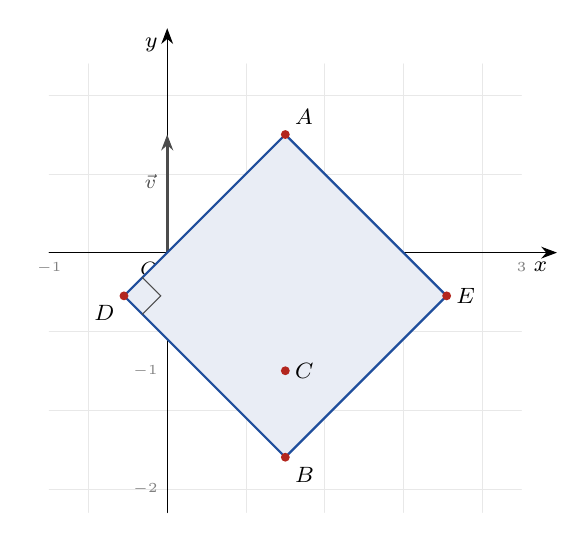
\begin{tikzpicture}[x=1.50cm,y=1.50cm,font=\footnotesize,line cap=round]
\draw[gray!18,very thin] (-1,-2.2) grid (3,1.6);
\draw[-{Stealth[length=2mm]}] (-1,0)--(3.3,0) node[below left]{$x$};
\draw[-{Stealth[length=2mm]}] (0,-2.2)--(0,1.9) node[below left]{$y$};
\node[below left,font=\scriptsize] at (0,0){$O$};
\draw[-{Stealth[length=2mm]},very thick,black!70] (0,0)--(1,0) node[pos=.6,below,font=\scriptsize]{$\vec u$};
\draw[-{Stealth[length=2mm]},very thick,black!70] (0,0)--(0,1) node[pos=.6,left,font=\scriptsize]{$\vec v$};
\node[below,font=\tiny,gray] at (-1,0){$-1$};
\node[below,font=\tiny,gray] at (2,0){$2$};
\node[below,font=\tiny,gray] at (3,0){$3$};
\node[left,font=\tiny,gray] at (0,-2){$-2$};
\node[left,font=\tiny,gray] at (0,-1){$-1$};
\begin{scope}\clip (-1,-2.2) rectangle (3.2,1.8);
\fill[cDef!10] (1.0000,1.0000)--(2.3660,-0.3660)--(1.0000,-1.7321)--(-0.3660,-0.3660)--cycle;\draw[cDef,thick] (1.0000,1.0000)--(2.3660,-0.3660)--(1.0000,-1.7321)--(-0.3660,-0.3660)--cycle;\draw[black!70] (-0.2105,-0.2105)--(-0.0549,-0.3660)--(-0.2105,-0.5216);
\end{scope}
\fill[cThm] (1.0000,1.0000) circle (1.6pt) node[above right,text=black]{$A$};
\fill[cThm] (1.0000,-1.7321) circle (1.6pt) node[below right,text=black]{$B$};
\fill[cThm] (1.0000,-1.0000) circle (1.6pt) node[right,text=black]{$C$};
\fill[cThm] (-0.3660,-0.3660) circle (1.6pt) node[below left,text=black]{$D$};
\fill[cThm] (2.3660,-0.3660) circle (1.6pt) node[right,text=black]{$E$};
\end{tikzpicture}\end{LTR}\end{center}
\end{hal}

% ===================== التمرين 2 =====================
\begin{tamrin}{بكالوريا 2026 -- الموضوع الثاني -- شعبة رياضيات}
$\theta$ عدد حقيقي حيث: $-\dfrac{\pi}{2}<\theta<\dfrac{\pi}{2}$.

\QQ{1} حل في المجموعة $\mathbb{C}$ المعادلة ذات المجهول $z$ التالية: $\left(z-i\sqrt3\right)\left(z^2-4(\sin\theta)z+4\right)=0$.

\QQ{2} في المستوي المركب المنسوب إلى المعلم المتعامد والمتجانس $\left(O;\vec u,\vec v\right)$، نعتبر النقط $A$، $B$، $C$ و$D$ لاحقاتها على الترتيب $z_A$، $z_B$، $z_C$ و$z_D$ حيث:
\[z_A=i\sqrt3,\quad z_B=2(\sin\theta+i\cos\theta),\quad z_C=2(\sin\theta-i\cos\theta),\quad z_D=1+i\sqrt3.\]
\begin{sq}
\qa أكتب كلا من $z_A$، $z_B$، $z_C$ و$z_D$ على الشكل المثلثي.
\qb استنتج أن النقط $B$، $C$ و$D$ تنتمي إلى نفس الدائرة التي يطلب تعيين مركزها ونصف قطرها.
\qc بين أن: $\left(\dfrac{z_A}{\sqrt3}\right)^{2026}+\left(\dfrac{z_A}{\sqrt3}\right)^{1447}=-1-i$.
\qd عين قيم العدد $\theta$ حتى يكون المثلث $ABC$ قائما في $B$.
\end{sq}
\QQ{3} نضع $\theta=\dfrac{\pi}{6}$ ونعتبر العدد المركب $L$ حيث: $L=-(1+i)z_B$.
\begin{sq}
\qa أكتب $L$ على الشكل المثلثي وعلى الشكل الجبري.
\qb استنتج القيمة المضبوطة لكل من $\cos\dfrac{19\pi}{12}$ و$\sin\dfrac{19\pi}{12}$.
\end{sq}
\end{tamrin}
\begin{hal}
\QQ{1} المعادلة تكافئ $z=i\sqrt3$ أو $z^2-4(\sin\theta)z+4=0$.

مميز المعادلة الثانية: $\Delta=16\sin^2\theta-16=-16\left(1-\sin^2\theta\right)=-16\cos^2\theta=\left(4i\cos\theta\right)^2$.
بما أن $-\frac{\pi}{2}<\theta<\frac{\pi}{2}$ فإن $\cos\theta>0$ ومنه $\Delta<0$، فللمعادلة حلان مترافقان:
\[z_1=\frac{4\sin\theta+4i\cos\theta}{2}=2(\sin\theta+i\cos\theta),\qquad z_2=\overline{z_1}=2(\sin\theta-i\cos\theta).\]
\[\bx{S=\left\{i\sqrt3\,;\,2(\sin\theta+i\cos\theta)\,;\,2(\sin\theta-i\cos\theta)\right\}}\]

\QQ{2}\pa
\begin{itemize}
\item $z_A=i\sqrt3$: \bx{z_A=\sqrt3\left(\cos\frac{\pi}{2}+i\sin\frac{\pi}{2}\right)}
\item نعلم أن $\sin\theta=\cos\left(\frac{\pi}{2}-\theta\right)$ و$\cos\theta=\sin\left(\frac{\pi}{2}-\theta\right)$، و$2>0$، إذن:
\bx{z_B=2\left(\cos\left(\frac{\pi}{2}-\theta\right)+i\sin\left(\frac{\pi}{2}-\theta\right)\right)}
\item $z_C=\overline{z_B}$: \bx{z_C=2\left(\cos\left(\theta-\frac{\pi}{2}\right)+i\sin\left(\theta-\frac{\pi}{2}\right)\right)}
\item $|z_D|=\sqrt{1+3}=2$: \bx{z_D=2\left(\cos\frac{\pi}{3}+i\sin\frac{\pi}{3}\right)}
\end{itemize}
\pb $|z_B|=|z_C|=|z_D|=2$، أي $OB=OC=OD=2$، إذن:\par\bxt{$B$، $C$ و$D$ تنتمي إلى الدائرة التي مركزها $O$ ونصف قطرها $2$}.

\pc $\dfrac{z_A}{\sqrt3}=i$، و$2026=4\times506+2$، $1447=4\times361+3$، ومنه:
\[\left(\frac{z_A}{\sqrt3}\right)^{2026}+\left(\frac{z_A}{\sqrt3}\right)^{1447}=i^{2026}+i^{1447}=\left(i^4\right)^{506}i^2+\left(i^4\right)^{361}i^3=-1-i.\quad\textcolor{cRem}{\checkmark}\]

\pd $z_C-z_B=-4i\cos\theta$ وهو تخيلي صرف غير معدوم ($\cos\theta\neq0$)، إذن المستقيم $(BC)$ يوازي محور التراتيب.
المثلث $ABC$ قائم في $B$ يعني $(BA)\perp(BC)$، أي $(BA)$ يوازي محور الفواصل، أي $\operatorname{Im}(z_A)=\operatorname{Im}(z_B)$ و$A\neq B$:
$2\cos\theta=\sqrt3$ أي $\cos\theta=\frac{\sqrt3}{2}$، ومع $\theta\in\left]-\frac{\pi}{2};\frac{\pi}{2}\right[$ نجد $\theta=\frac{\pi}{6}$ أو $\theta=-\frac{\pi}{6}$.

وفي الحالتين $\operatorname{Re}(z_B)=2\sin\theta=\pm1\neq0=\operatorname{Re}(z_A)$ أي $A\neq B$. للتأكد: $\dfrac{z_A-z_B}{z_C-z_B}=\mp\dfrac{\sqrt3}{6}i$ تخيلي صرف.
إذن: \bx{\theta=\frac{\pi}{6}} أو \bx{\theta=-\frac{\pi}{6}}

\QQ{3} من أجل $\theta=\frac{\pi}{6}$: $z_B=2\left(\frac12+i\frac{\sqrt3}{2}\right)=1+i\sqrt3=2e^{i\frac{\pi}{3}}$ (أي $B=D$).

\pa $-(1+i)=\sqrt2\left(-\frac{\sqrt2}{2}-i\frac{\sqrt2}{2}\right)=\sqrt2\left(\cos\frac{5\pi}{4}+i\sin\frac{5\pi}{4}\right)$، إذن
$|L|=\sqrt2\times2=2\sqrt2$ و$\arg L=\frac{5\pi}{4}+\frac{\pi}{3}=\frac{19\pi}{12}$:
\[\bx{L=2\sqrt2\left(\cos\frac{19\pi}{12}+i\sin\frac{19\pi}{12}\right)}\]
الشكل الجبري: $L=-(1+i)(1+i\sqrt3)=-\left(1+i\sqrt3+i-\sqrt3\right)=\bx{\left(\sqrt3-1\right)-i\left(1+\sqrt3\right)}$

\pb بالمطابقة: $2\sqrt2\cos\frac{19\pi}{12}=\sqrt3-1$ و$2\sqrt2\sin\frac{19\pi}{12}=-(1+\sqrt3)$، ومنه:
\[\bx{\cos\frac{19\pi}{12}=\frac{\sqrt6-\sqrt2}{4}}\qquad\bx{\sin\frac{19\pi}{12}=-\frac{\sqrt6+\sqrt2}{4}}\]
الشكل من أجل $\theta=\frac{\pi}{6}$ (الدائرة $\mathcal{C}(O;2)$ والزاوية القائمة في $B$):
\begin{center}\begin{LTR}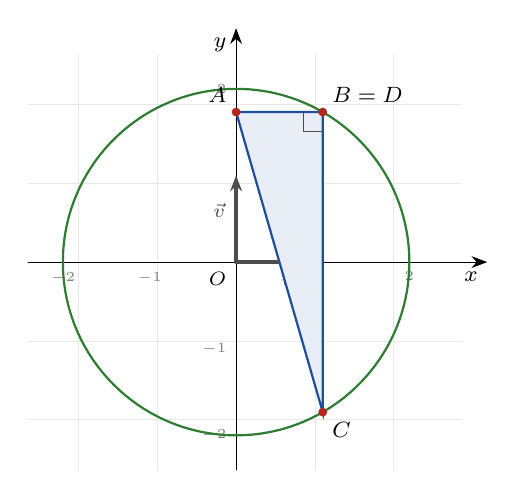
\begin{tikzpicture}[x=1.10cm,y=1.10cm,font=\footnotesize,line cap=round]
\draw[gray!18,very thin] (-2.4,-2.4) grid (2.6,2.4);
\draw[-{Stealth[length=2mm]}] (-2.4,0)--(2.9,0) node[below left]{$x$};
\draw[-{Stealth[length=2mm]}] (0,-2.4)--(0,2.7) node[below left]{$y$};
\node[below left,font=\scriptsize] at (0,0){$O$};
\draw[-{Stealth[length=2mm]},very thick,black!70] (0,0)--(1,0) node[pos=.6,below,font=\scriptsize]{$\vec u$};
\draw[-{Stealth[length=2mm]},very thick,black!70] (0,0)--(0,1) node[pos=.6,left,font=\scriptsize]{$\vec v$};
\node[below,font=\tiny,gray] at (-2,0){$-2$};
\node[below,font=\tiny,gray] at (-1,0){$-1$};
\node[below,font=\tiny,gray] at (2,0){$2$};
\node[left,font=\tiny,gray] at (0,-2){$-2$};
\node[left,font=\tiny,gray] at (0,-1){$-1$};
\node[left,font=\tiny,gray] at (0,2){$2$};
\begin{scope}\clip (-2.4,-2.4) rectangle (2.8,2.6);
\draw[cRem,thick] (0,0) circle (2);\fill[cDef!10] (0.0000,1.7321)--(1.0000,1.7321)--(1.0000,-1.7321)--cycle;\draw[cDef,thick] (0.0000,1.7321)--(1.0000,1.7321)--(1.0000,-1.7321)--cycle;\draw[black!70] (0.7800,1.7321)--(0.7800,1.5121)--(1.0000,1.5121);
\end{scope}
\fill[cThm] (0.0000,1.7321) circle (1.6pt) node[above left,text=black]{$A$};
\fill[cThm] (1.0000,1.7321) circle (1.6pt) node[above right,text=black]{$B=D$};
\fill[cThm] (1.0000,-1.7321) circle (1.6pt) node[below right,text=black]{$C$};
\end{tikzpicture}\end{LTR}\end{center}
\end{hal}

% ===================== التمرين 3 =====================
\begin{tamrin}{بكالوريا 2025 -- الموضوع الأول -- شعبة رياضيات}
\QQ{1} حل في مجموعة الأعداد المركبة $\mathbb{C}$ المعادلة ذات المجهول $z$ التالية: $\left(z^2+1\right)\left(z^2-6z+13\right)=0$.

\QQ{2} المستوي المركب منسوب إلى المعلم المتعامد والمتجانس $\left(O;\vec u,\vec v\right)$.
$A$، $B$ و$C$ نقط من المستوي لاحقاتها على الترتيب $z_A$، $z_B$ و$z_C$ حيث: $z_A=2-3i$، $z_B=iz_A$ و$z_C=-i$،
و$L$ عدد مركب حيث: $L=\dfrac{z_A-z_C}{z_B-z_C}$.
\begin{sq}
\qa أكتب كلا من العددين $z_A-z_C$ و$z_B-z_C$ على الشكل المثلثي.
\qb عين الطويلة وعمدة للعدد المركب $L$ ثم حدد طبيعة المثلث $ABC$.
\qc بين أن النقط $O$، $A$، $B$ و$C$ تنتمي إلى نفس الدائرة التي يطلب تعيين مركزها ونصف قطرها.
\qd من أجل كل عدد طبيعي $n$، نضع: $S_n=|L|+|L|^2+\cdots+|L|^n$.

أحسب بدلالة $n$ المجموع $S_n$ ثم استنتج $\displaystyle\lim_{n\to+\infty}S_n$.
\end{sq}
\QQ{3} $z_\theta$ عدد مركب حيث: $z_\theta=1+\cos2\theta-i\sin2\theta$ و$\theta$ عدد حقيقي يختلف عن $\dfrac{\pi}{2}$ مع $0<\theta<\pi$.

بين أن: $z_\theta=2\cos\theta\left(\cos\theta-i\sin\theta\right)$ ثم استنتج حسب قيم $\theta$ الطويلة وعمدة للعدد $z_\theta$.
\end{tamrin}
\begin{hal}
\QQ{1} $z^2+1=0\iff z^2=i^2\iff z=i$ أو $z=-i$.

$z^2-6z+13=0$: $\Delta=36-52=-16=(4i)^2$، ومنه $z=\dfrac{6\pm4i}{2}$، أي $z=3+2i$ أو $z=3-2i$.
\[\bx{S=\left\{-i\,;\,i\,;\,3-2i\,;\,3+2i\right\}}\]
\QQ{2} $z_B=i(2-3i)=3+2i$.

\pa $z_A-z_C=2-3i+i=2-2i=2\sqrt2\left(\frac{\sqrt2}{2}-i\frac{\sqrt2}{2}\right)$: \bx{z_A-z_C=2\sqrt2\left(\cos\left(-\frac{\pi}{4}\right)+i\sin\left(-\frac{\pi}{4}\right)\right)}

$z_B-z_C=3+3i=3\sqrt2\left(\frac{\sqrt2}{2}+i\frac{\sqrt2}{2}\right)$: \bx{z_B-z_C=3\sqrt2\left(\cos\frac{\pi}{4}+i\sin\frac{\pi}{4}\right)}

\pb $|L|=\dfrac{2\sqrt2}{3\sqrt2}=\bx{\dfrac23}$ و$\arg L=-\dfrac{\pi}{4}-\dfrac{\pi}{4}=\bx{-\dfrac{\pi}{2}}$، أي $L=-\frac23 i$.

إذن $\left(\overrightarrow{CB};\overrightarrow{CA}\right)=-\frac{\pi}{2}+2k\pi$ و$\frac{CA}{CB}=\frac23\neq1$:
\bxt{المثلث $ABC$ قائم في $C$ (وليس متساوي الساقين)}.

\pc المثلث $ABC$ قائم في $C$، إذن $C$ تنتمي إلى الدائرة ذات القطر $[AB]$.
ومن جهة أخرى $\dfrac{z_B}{z_A}=i$، أي $\left(\overrightarrow{OA};\overrightarrow{OB}\right)=\frac{\pi}{2}+2k\pi$، فالمثلث $OAB$ قائم في $O$، إذن $O$ تنتمي أيضا إلى الدائرة ذات القطر $[AB]$.

مركزها $\Omega$ منتصف $[AB]$: $z_\Omega=\dfrac{z_A+z_B}{2}=\bx{\dfrac52-\dfrac12 i}$، ونصف قطرها $r=\dfrac{AB}{2}=\dfrac{|1+5i|}{2}=\bx{\dfrac{\sqrt{26}}{2}}$.
\begin{center}\begin{LTR}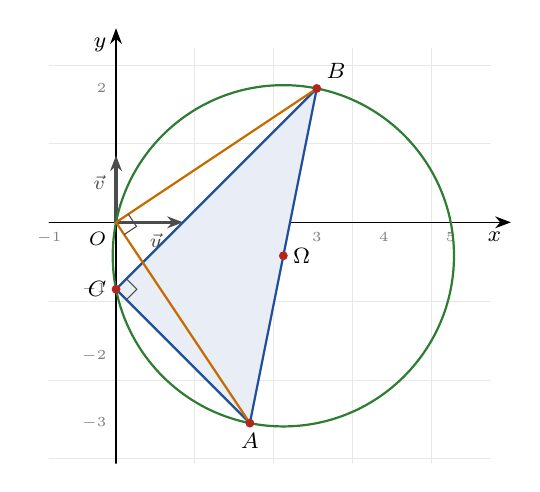
\begin{tikzpicture}[x=0.85cm,y=0.85cm,font=\footnotesize,line cap=round]
\draw[gray!18,very thin] (-1,-3.6) grid (5.6,2.6);
\draw[-{Stealth[length=2mm]}] (-1,0)--(5.9,0) node[below left]{$x$};
\draw[-{Stealth[length=2mm]}] (0,-3.6)--(0,2.9) node[below left]{$y$};
\node[below left,font=\scriptsize] at (0,0){$O$};
\draw[-{Stealth[length=2mm]},very thick,black!70] (0,0)--(1,0) node[pos=.6,below,font=\scriptsize]{$\vec u$};
\draw[-{Stealth[length=2mm]},very thick,black!70] (0,0)--(0,1) node[pos=.6,left,font=\scriptsize]{$\vec v$};
\node[below,font=\tiny,gray] at (-1,0){$-1$};
\node[below,font=\tiny,gray] at (2,0){$2$};
\node[below,font=\tiny,gray] at (3,0){$3$};
\node[below,font=\tiny,gray] at (4,0){$4$};
\node[below,font=\tiny,gray] at (5,0){$5$};
\node[left,font=\tiny,gray] at (0,-3){$-3$};
\node[left,font=\tiny,gray] at (0,-2){$-2$};
\node[left,font=\tiny,gray] at (0,-1){$-1$};
\node[left,font=\tiny,gray] at (0,2){$2$};
\begin{scope}\clip (-1,-3.6) rectangle (5.8,2.8);
\draw[cRem,thick] (2.5,-.5) circle (2.5495);\fill[cDef!10] (2.0000,-3.0000)--(3.0000,2.0000)--(0.0000,-1.0000)--cycle;\draw[cDef,thick] (2.0000,-3.0000)--(3.0000,2.0000)--(0.0000,-1.0000)--cycle;\draw[black!70] (0.1556,-1.1556)--(0.3111,-1.0000)--(0.1556,-0.8444);\draw[cEx,thick] (2,-3)--(0,0)--(3,2);\draw[black!70] (0.1220,-0.1831)--(0.3051,-0.0610)--(0.1831,0.1220);
\end{scope}
\fill[cThm] (2.0000,-3.0000) circle (1.6pt) node[below,text=black]{$A$};
\fill[cThm] (3.0000,2.0000) circle (1.6pt) node[above right,text=black]{$B$};
\fill[cThm] (0.0000,-1.0000) circle (1.6pt) node[left,text=black]{$C$};
\fill[cThm] (2.5000,-0.5000) circle (1.6pt) node[right,text=black]{$\Omega$};
\end{tikzpicture}\end{LTR}\end{center}
\pd $S_n$ مجموع $n$ حدا متتابعا من متتالية هندسية أساسها $q=|L|=\frac23\neq1$ وحدها الأول $\frac23$:
\[S_n=\frac23\times\frac{1-\left(\frac23\right)^n}{1-\frac23}=\bx{2\left(1-\left(\frac23\right)^n\right)}\]
بما أن $0<\frac23<1$ فإن $\displaystyle\lim_{n\to+\infty}\left(\frac23\right)^n=0$، ومنه \bx{\lim_{n\to+\infty}S_n=2}

\QQ{3} نعلم أن $1+\cos2\theta=2\cos^2\theta$ و$\sin2\theta=2\sin\theta\cos\theta$، إذن:
\[z_\theta=2\cos^2\theta-2i\sin\theta\cos\theta=2\cos\theta\left(\cos\theta-i\sin\theta\right)=2\cos\theta\, e^{-i\theta}.\quad\textcolor{cRem}{\checkmark}\]
\begin{itemize}
\item إذا كان $0<\theta<\frac{\pi}{2}$: $\cos\theta>0$، إذن \bx{|z_\theta|=2\cos\theta,\ \ \arg z_\theta=-\theta+2k\pi}
\item إذا كان $\frac{\pi}{2}<\theta<\pi$: $\cos\theta<0$، فنكتب $z_\theta=(-2\cos\theta)\left(-e^{-i\theta}\right)=(-2\cos\theta)\,e^{i(\pi-\theta)}$، إذن
\bx{|z_\theta|=-2\cos\theta,\ \ \arg z_\theta=\pi-\theta+2k\pi}
\end{itemize}
\end{hal}

% ===================== التمرين 4 =====================
\begin{tamrin}{بكالوريا 2025 -- الموضوع الثاني -- شعبة رياضيات}
\QQ{1} حل في مجموعة الأعداد المركبة $\mathbb{C}$ المعادلة ذات المجهول $z$ التالية: $\left(iz-1+2i\right)\left(z^2-4z+5\right)=0$.

\QQ{2} المستوي المركب منسوب إلى المعلم المتعامد والمتجانس $\left(O;\vec u,\vec v\right)$.
$A$، $B$ و$C$ نقط من المستوي لاحقاتها على الترتيب $z_A$، $z_B$ و$z_C$ حيث: $z_A=2-i$، $z_B=\overline{z_A}$ و$z_C=-2-i$،
و$L$ عدد مركب حيث: $L=\dfrac{z_C-z_A}{z_B-z_A}$.
\begin{sq}
\qa أكتب العدد $L$ على الشكل المثلثي ثم حدد طبيعة المثلث $ABC$.
\qb بين أن النقط $A$، $B$ و$C$ تنتمي إلى نفس الدائرة التي يطلب تعيين مركزها ونصف قطرها.
\qc عين $z_D$ و$z_E$ لاحقتي النقطتين $D$ و$E$ على الترتيب حتى يكون الرباعي $BCDE$ معينا مركزه $A$.
\end{sq}
\QQ{3} $z_\theta$ عدد مركب حيث: $z_\theta=1-\cos2\theta+i\sin2\theta$ و$\theta$ عدد حقيقي غير معدوم مع $-\dfrac{\pi}{2}<\theta<\dfrac{\pi}{2}$.

بين أن: $z_\theta=2\sin\theta\left(\sin\theta+i\cos\theta\right)$ ثم استنتج حسب قيم $\theta$ الطويلة وعمدة للعدد $z_\theta$.
\end{tamrin}
\begin{hal}
\QQ{1} $iz-1+2i=0\iff z=\dfrac{1-2i}{i}=\dfrac{(1-2i)(-i)}{1}=-2-i$.

$z^2-4z+5=0$: $\Delta=16-20=-4=(2i)^2$، ومنه $z=2+i$ أو $z=2-i$.
\[\bx{S=\left\{-2-i\,;\,2-i\,;\,2+i\right\}}\]
\QQ{2}\pa $z_B=2+i$، $z_C-z_A=-4$ و$z_B-z_A=2i$، ومنه $L=\dfrac{-4}{2i}=2i$:
\bx{L=2\left(\cos\frac{\pi}{2}+i\sin\frac{\pi}{2}\right)}

إذن $\frac{AC}{AB}=2$ و$\left(\overrightarrow{AB};\overrightarrow{AC}\right)=\frac{\pi}{2}+2k\pi$: \bxt{المثلث $ABC$ قائم في $A$ (و$AC=2AB$)}.

\pb المثلث $ABC$ قائم في $A$، فالنقط $A$، $B$، $C$ تنتمي إلى الدائرة ذات القطر $[BC]$؛ مركزها منتصف $[BC]$: $\dfrac{z_B+z_C}{2}=\dfrac{2+i-2-i}{2}=0$ أي النقطة $O$،
ونصف قطرها $\dfrac{BC}{2}=\dfrac{|-4-2i|}{2}=\dfrac{2\sqrt5}{2}=\sqrt5$ (وفعلا $|z_A|=|z_B|=|z_C|=\sqrt5$).
\begin{center}\bxt{الدائرة التي مركزها $O$ ونصف قطرها $\sqrt5$}\end{center}
\pc يكون $BCDE$ متوازي أضلاع مركزه $A$ إذا وفقط إذا كانت $A$ منتصف القطرين $[BD]$ و$[CE]$:
\[z_D=2z_A-z_B=4-2i-2-i=\bx{2-3i},\qquad z_E=2z_A-z_C=4-2i+2+i=\bx{6-i}\]
وبما أن قطريه $[BD]$ و$[CE]$ متعامدان (لأن $(AB)\perp(AC)$) فإن $BCDE$ معين مركزه $A$.
\begin{center}\begin{LTR}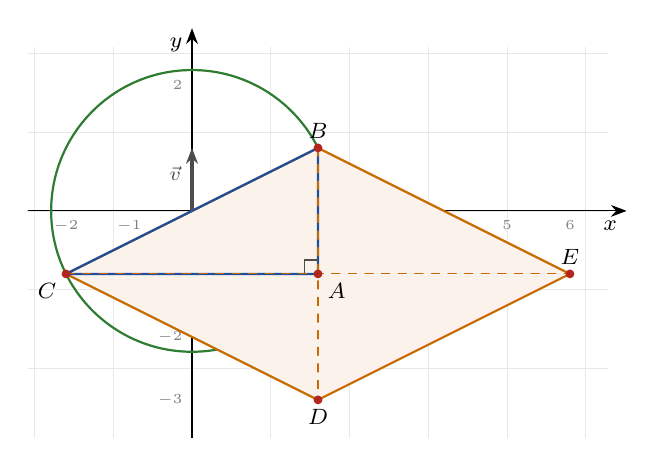
\begin{tikzpicture}[x=0.80cm,y=0.80cm,font=\footnotesize,line cap=round]
\draw[gray!18,very thin] (-2.6,-3.6) grid (6.6,2.6);
\draw[-{Stealth[length=2mm]}] (-2.6,0)--(6.9,0) node[below left]{$x$};
\draw[-{Stealth[length=2mm]}] (0,-3.6)--(0,2.9) node[below left]{$y$};
\node[below left,font=\scriptsize] at (0,0){$O$};
\draw[-{Stealth[length=2mm]},very thick,black!70] (0,0)--(1,0) node[pos=.6,below,font=\scriptsize]{$\vec u$};
\draw[-{Stealth[length=2mm]},very thick,black!70] (0,0)--(0,1) node[pos=.6,left,font=\scriptsize]{$\vec v$};
\node[below,font=\tiny,gray] at (-2,0){$-2$};
\node[below,font=\tiny,gray] at (-1,0){$-1$};
\node[below,font=\tiny,gray] at (2,0){$2$};
\node[below,font=\tiny,gray] at (3,0){$3$};
\node[below,font=\tiny,gray] at (4,0){$4$};
\node[below,font=\tiny,gray] at (5,0){$5$};
\node[below,font=\tiny,gray] at (6,0){$6$};
\node[left,font=\tiny,gray] at (0,-3){$-3$};
\node[left,font=\tiny,gray] at (0,-2){$-2$};
\node[left,font=\tiny,gray] at (0,-1){$-1$};
\node[left,font=\tiny,gray] at (0,2){$2$};
\begin{scope}\clip (-2.6,-3.6) rectangle (6.8,2.8);
\draw[cRem,thick] (0,0) circle (2.2361);\fill[cEx!8] (2.0000,1.0000)--(-2.0000,-1.0000)--(2.0000,-3.0000)--(6.0000,-1.0000)--cycle;\draw[cEx,thick] (2.0000,1.0000)--(-2.0000,-1.0000)--(2.0000,-3.0000)--(6.0000,-1.0000)--cycle;\draw[cDef,thick] (2.0000,-1.0000)--(2.0000,1.0000)--(-2.0000,-1.0000)--cycle;\draw[black!70] (2.0000,-0.7800)--(1.7800,-0.7800)--(1.7800,-1.0000);\draw[cEx,dashed] (2,1)--(2,-3) (-2,-1)--(6,-1);
\end{scope}
\fill[cThm] (2.0000,-1.0000) circle (1.6pt) node[below right,text=black]{$A$};
\fill[cThm] (2.0000,1.0000) circle (1.6pt) node[above,text=black]{$B$};
\fill[cThm] (-2.0000,-1.0000) circle (1.6pt) node[below left,text=black]{$C$};
\fill[cThm] (2.0000,-3.0000) circle (1.6pt) node[below,text=black]{$D$};
\fill[cThm] (6.0000,-1.0000) circle (1.6pt) node[above,text=black]{$E$};
\end{tikzpicture}\end{LTR}\end{center}
\QQ{3} $1-\cos2\theta=2\sin^2\theta$ و$\sin2\theta=2\sin\theta\cos\theta$، إذن:
\[z_\theta=2\sin^2\theta+2i\sin\theta\cos\theta=2\sin\theta\left(\sin\theta+i\cos\theta\right).\quad\textcolor{cRem}{\checkmark}\]
و$\sin\theta+i\cos\theta=\cos\left(\frac{\pi}{2}-\theta\right)+i\sin\left(\frac{\pi}{2}-\theta\right)=e^{i\left(\frac{\pi}{2}-\theta\right)}$.
\begin{itemize}
\item إذا كان $0<\theta<\frac{\pi}{2}$: $\sin\theta>0$، إذن \bx{|z_\theta|=2\sin\theta,\ \ \arg z_\theta=\frac{\pi}{2}-\theta+2k\pi}
\item إذا كان $-\frac{\pi}{2}<\theta<0$: $\sin\theta<0$، فنكتب $z_\theta=(-2\sin\theta)\,e^{i\pi}e^{i\left(\frac{\pi}{2}-\theta\right)}$، إذن
\bx{|z_\theta|=-2\sin\theta,\ \ \arg z_\theta=-\frac{\pi}{2}-\theta+2k\pi}
\end{itemize}
\end{hal}

% ===================== التمرين 5 =====================
\begin{tamrin}{بكالوريا 2024 -- الموضوع الأول -- شعبة رياضيات}
\textbf{I)} حل في مجموعة الأعداد المركبة $\mathbb{C}$ المعادلة ذات المجهول $z$ الآتية: $\left(z-8+6i\right)\left(z^2-2z+4\right)=0$.
\textbf{II)} المستوي المركب منسوب إلى المعلم المتعامد والمتجانس $\left(O;\vec i,\vec j\right)$.
نعتبر النقط $A$، $B$ و$C$ التي لاحقاتها على الترتيب $z_A$، $z_B$ و$z_C$ حيث: $z_A=1+i\sqrt3$، $z_B=iz_A$ و$z_C=-z_A$.

\QQ{1} تحقق أن: $z_A-z_B=i\left(z_C-z_B\right)$ ثم بين أن المثلث $ABC$ قائم ومتساوي الساقين.

\QQ{2}
\begin{sq}
\qa أكتب كلا من $z_A$، $z_B$ و$z_C$ على الشكل المثلثي.
\qb استنتج أن النقط $A$، $B$ و$C$ تنتمي إلى نفس الدائرة، يطلب تعيين مركزها ونصف قطرها.
\end{sq}
\QQ{3} النقطة $D$ هي نظيرة $B$ بالنسبة إلى مبدأ المعلم. بين أن الرباعي $ABCD$ مربع.
\begin{molahada}
حُذف السؤال I(ب) «جد الجذرين التربيعيين للعدد المركب $8-6i$» لأنه خارج المنهاج الحالي (التوزيع السنوي 2026-2027): الجذران التربيعيان لعدد مركب مقرران في شعبة علوم تجريبية فقط.
\end{molahada}
\end{tamrin}
\begin{hal}
\textbf{I)} $z-8+6i=0\iff z=8-6i$.

$z^2-2z+4=0$: $\Delta=4-16=-12=\left(2i\sqrt3\right)^2$، ومنه $z=\dfrac{2\pm2i\sqrt3}{2}=1\pm i\sqrt3$.
\[\bx{S=\left\{8-6i\,;\,1-i\sqrt3\,;\,1+i\sqrt3\right\}}\]
\textbf{II)} $z_B=i\left(1+i\sqrt3\right)=-\sqrt3+i$ و$z_C=-1-i\sqrt3$.

\QQ{1} $z_A-z_B=\left(1+\sqrt3\right)+i\left(\sqrt3-1\right)$ و$z_C-z_B=\left(\sqrt3-1\right)-i\left(1+\sqrt3\right)$،
ومنه $i\left(z_C-z_B\right)=\left(1+\sqrt3\right)+i\left(\sqrt3-1\right)=z_A-z_B$. \ok

إذن $\dfrac{z_A-z_B}{z_C-z_B}=i$: $BA=BC$ و$\left(\overrightarrow{BC};\overrightarrow{BA}\right)=\frac{\pi}{2}+2k\pi$،
أي \bxt{المثلث $ABC$ قائم في $B$ ومتساوي الساقين}.

\QQ{2}\pa $|z_A|=2$ و$z_A=2\left(\frac12+i\frac{\sqrt3}{2}\right)$: \bx{z_A=2\left(\cos\frac{\pi}{3}+i\sin\frac{\pi}{3}\right)}

$z_B=e^{i\frac{\pi}{2}}z_A$: \bx{z_B=2\left(\cos\frac{5\pi}{6}+i\sin\frac{5\pi}{6}\right)}

$z_C=e^{i\pi}z_A$: \bx{z_C=2\left(\cos\left(-\frac{2\pi}{3}\right)+i\sin\left(-\frac{2\pi}{3}\right)\right)}

\pb $OA=OB=OC=2$: \bxt{$A$، $B$ و$C$ تنتمي إلى الدائرة التي مركزها $O$ ونصف قطرها $2$}.

\QQ{3} $z_D=-z_B=\sqrt3-i$. لدينا $\frac{z_A+z_C}{2}=0$ و$\frac{z_B+z_D}{2}=0$: القطران $[AC]$ و$[BD]$ لهما نفس المنتصف $O$، إذن $ABCD$ متوازي أضلاع.
وزيادة على ذلك $AC=BD=4$ (قطرا الدائرة) و$\dfrac{z_B}{z_A}=i$ أي $(OA)\perp(OB)$ فالقطران متعامدان.
متوازي أضلاع قطراه متقايسان ومتعامدان، إذن \bxt{الرباعي $ABCD$ مربع}.
\begin{center}\begin{LTR}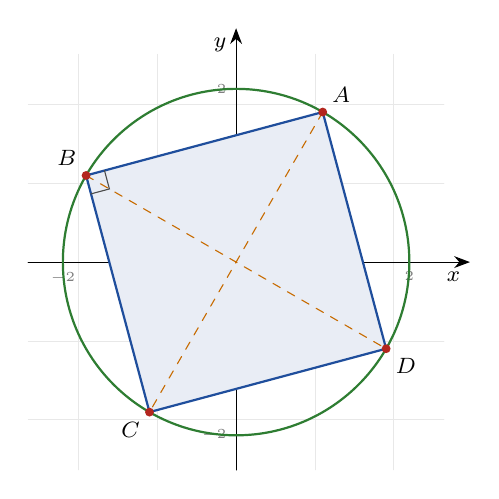
\begin{tikzpicture}[x=1.10cm,y=1.10cm,font=\footnotesize,line cap=round]
\draw[gray!18,very thin] (-2.4,-2.4) grid (2.4,2.4);
\draw[-{Stealth[length=2mm]}] (-2.4,0)--(2.7,0) node[below left]{$x$};
\draw[-{Stealth[length=2mm]}] (0,-2.4)--(0,2.7) node[below left]{$y$};
\node[below left,font=\scriptsize] at (0,0){$O$};
\draw[-{Stealth[length=2mm]},very thick,black!70] (0,0)--(1,0) node[pos=.6,below,font=\scriptsize]{$\vec u$};
\draw[-{Stealth[length=2mm]},very thick,black!70] (0,0)--(0,1) node[pos=.6,left,font=\scriptsize]{$\vec v$};
\node[below,font=\tiny,gray] at (-2,0){$-2$};
\node[below,font=\tiny,gray] at (-1,0){$-1$};
\node[below,font=\tiny,gray] at (2,0){$2$};
\node[left,font=\tiny,gray] at (0,-2){$-2$};
\node[left,font=\tiny,gray] at (0,-1){$-1$};
\node[left,font=\tiny,gray] at (0,2){$2$};
\begin{scope}\clip (-2.4,-2.4) rectangle (2.6,2.6);
\draw[cRem,thick] (0,0) circle (2);\fill[cDef!10] (1.0000,1.7321)--(-1.7321,1.0000)--(-1.0000,-1.7321)--(1.7321,-1.0000)--cycle;\draw[cDef,thick] (1.0000,1.7321)--(-1.7321,1.0000)--(-1.0000,-1.7321)--(1.7321,-1.0000)--cycle;\draw[black!70] (-1.5195,1.0569)--(-1.4626,0.8444)--(-1.6751,0.7875);\draw[cEx,dashed] (1,1.7321)--(-1,-1.7321) (-1.7321,1)--(1.7321,-1);
\end{scope}
\fill[cThm] (1.0000,1.7321) circle (1.6pt) node[above right,text=black]{$A$};
\fill[cThm] (-1.7321,1.0000) circle (1.6pt) node[above left,text=black]{$B$};
\fill[cThm] (-1.0000,-1.7321) circle (1.6pt) node[below left,text=black]{$C$};
\fill[cThm] (1.7321,-1.0000) circle (1.6pt) node[below right,text=black]{$D$};
\end{tikzpicture}\end{LTR}\end{center}
\end{hal}

% ===================== التمرين 6 =====================
\begin{tamrin}{بكالوريا 2024 -- الموضوع الثاني -- شعبة رياضيات}
\textbf{I)} حل في مجموعة الأعداد المركبة $\mathbb{C}$ المعادلة ذات المجهول $z$ الآتية: $\left(z^2+2i\right)\left(z^2-2\sqrt3z+6\right)=0$.

\textbf{II)} المستوي المركب منسوب إلى المعلم المتعامد والمتجانس $\left(O;\vec i,\vec j\right)$.
نعتبر النقط $A$، $B$ و$C$ التي لاحقاتها على الترتيب $z_A$، $z_B$ و$z_C$ حيث: $z_A=1-i$، $z_B=-z_A$ و$z_C=\sqrt3(1+i)$.

\QQ{1} أكتب كلا من $z_A$، $z_B$ و$z_C$ على الشكل المثلثي.

\QQ{2} أكتب العدد المركب $\dfrac{z_C-z_A}{z_B-z_A}$ على الشكل الجبري ثم المثلثي وبين أن المثلث $ABC$ متقايس الأضلاع.

\QQ{3}
\begin{sq}
\qa عين لاحقة النقطة $G$ مركز الدائرة المحيطة بالمثلث $ABC$ ثم أحسب نصف قطرها.
\qb النقطة $D$ هي نظيرة $C$ بالنسبة إلى مبدأ المعلم. بين أن الرباعي $ACBD$ معين.
\end{sq}
\end{tamrin}
\begin{molahada}
في نص الموضوع: «بين أن الرباعي $ABCD$ معين». لكن $O$ منتصف $[AB]$ ومنتصف $[CD]$، فقطرا المعين هما $[AB]$ و$[CD]$، والترتيب $A$، $B$، $C$، $D$ يعطي رباعيا متقاطع الأضلاع؛ لذلك صححنا التسمية إلى $ACBD$.
\end{molahada}
\begin{hal}
\textbf{I)} $z^2+2i=0\iff z^2=-2i=(1-i)^2$ (لأن $(1-i)^2=1-2i-1=-2i$)، ومنه $z=1-i$ أو $z=-1+i$.

$z^2-2\sqrt3z+6=0$: $\Delta=12-24=-12=\left(2i\sqrt3\right)^2$، ومنه $z=\dfrac{2\sqrt3\pm2i\sqrt3}{2}=\sqrt3\pm i\sqrt3$.
\[\bx{S=\left\{1-i\,;\,-1+i\,;\,\sqrt3+i\sqrt3\,;\,\sqrt3-i\sqrt3\right\}}\]
\textbf{II)}\QQ{1}
\bx{z_A=\sqrt2\left(\cos\left(-\frac{\pi}{4}\right)+i\sin\left(-\frac{\pi}{4}\right)\right)}،\quad
\bx{z_B=\sqrt2\left(\cos\frac{3\pi}{4}+i\sin\frac{3\pi}{4}\right)}

\bx{z_C=\sqrt6\left(\cos\frac{\pi}{4}+i\sin\frac{\pi}{4}\right)}\quad (لأن $\sqrt3(1+i)=\sqrt3\cdot\sqrt2\left(\frac{\sqrt2}{2}+i\frac{\sqrt2}{2}\right)$، و$z_B=e^{i\pi}z_A$).

\QQ{2} $z_C-z_A=\left(\sqrt3-1\right)+i\left(\sqrt3+1\right)$ و$z_B-z_A=-2+2i$:
\[\frac{z_C-z_A}{z_B-z_A}=\frac{\left[\left(\sqrt3-1\right)+i\left(\sqrt3+1\right)\right](-2-2i)}{(-2+2i)(-2-2i)}=\frac{4-4i\sqrt3}{8}=\bx{\frac12-i\frac{\sqrt3}{2}}\]
\[\frac{z_C-z_A}{z_B-z_A}=\bx{\cos\left(-\frac{\pi}{3}\right)+i\sin\left(-\frac{\pi}{3}\right)}\]
إذن $\frac{AC}{AB}=1$ و$\left(\overrightarrow{AB};\overrightarrow{AC}\right)=-\frac{\pi}{3}+2k\pi$: مثلث متساوي الساقين رأسه $A$ وزاويته الرئيسية $\frac{\pi}{3}$، إذن \bxt{المثلث $ABC$ متقايس الأضلاع}.

\QQ{3}\pa في المثلث المتقايس الأضلاع يتطابق مركز الدائرة المحيطة مع مركز الثقل:
\[z_G=\frac{z_A+z_B+z_C}{3}=\bx{\frac{\sqrt3}{3}(1+i)}\]
نصف القطر: $R=GA=\left|z_A-z_G\right|=\left|\left(1-\frac{\sqrt3}{3}\right)-i\left(1+\frac{\sqrt3}{3}\right)\right|=\sqrt{\left(1-\frac{\sqrt3}{3}\right)^2+\left(1+\frac{\sqrt3}{3}\right)^2}=\sqrt{2+\frac23}$، إذن \bx{R=\sqrt{\frac83}=\frac{2\sqrt6}{3}}

\pb $z_D=-z_C=-\sqrt3(1+i)$. منتصف $[AB]$ هو $O$ لأن $z_A+z_B=0$، ومنتصف $[CD]$ هو $O$ لأن $z_C+z_D=0$؛ إذن $ACBD$ متوازي أضلاع قطراه $[AB]$ و$[CD]$.
و$\dfrac{z_C}{z_A}=\dfrac{\sqrt3(1+i)}{1-i}=\sqrt3\,i$ تخيلي صرف، أي $(OA)\perp(OC)$: القطران متعامدان. إذن \bxt{الرباعي $ACBD$ معين}.
\begin{center}\begin{LTR}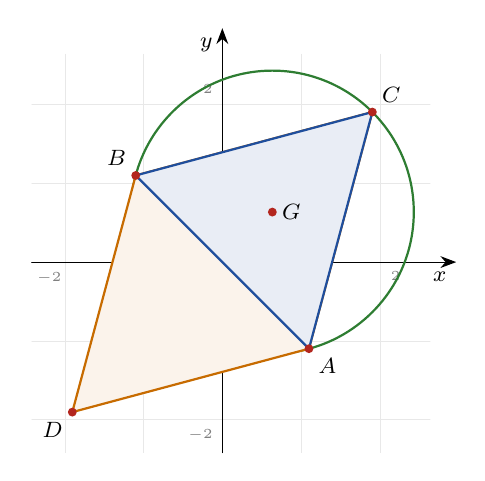
\begin{tikzpicture}[x=1.10cm,y=1.10cm,font=\footnotesize,line cap=round]
\draw[gray!18,very thin] (-2.2,-2.2) grid (2.4,2.4);
\draw[-{Stealth[length=2mm]}] (-2.2,0)--(2.7,0) node[below left]{$x$};
\draw[-{Stealth[length=2mm]}] (0,-2.2)--(0,2.7) node[below left]{$y$};
\node[below left,font=\scriptsize] at (0,0){$O$};
\draw[-{Stealth[length=2mm]},very thick,black!70] (0,0)--(1,0) node[pos=.6,below,font=\scriptsize]{$\vec u$};
\draw[-{Stealth[length=2mm]},very thick,black!70] (0,0)--(0,1) node[pos=.6,left,font=\scriptsize]{$\vec v$};
\node[below,font=\tiny,gray] at (-2,0){$-2$};
\node[below,font=\tiny,gray] at (-1,0){$-1$};
\node[below,font=\tiny,gray] at (2,0){$2$};
\node[left,font=\tiny,gray] at (0,-2){$-2$};
\node[left,font=\tiny,gray] at (0,-1){$-1$};
\node[left,font=\tiny,gray] at (0,2){$2$};
\begin{scope}\clip (-2.2,-2.2) rectangle (2.6,2.6);
\draw[cRem,thick] (0.5774,0.5774) circle (1.6330);\fill[cEx!8] (1.0000,-1.0000)--(1.7321,1.7321)--(-1.0000,1.0000)--(-1.7321,-1.7321)--cycle;\draw[cEx,thick] (1.0000,-1.0000)--(1.7321,1.7321)--(-1.0000,1.0000)--(-1.7321,-1.7321)--cycle;\fill[cDef!10] (1.0000,-1.0000)--(-1.0000,1.0000)--(1.7321,1.7321)--cycle;\draw[cDef,thick] (1.0000,-1.0000)--(-1.0000,1.0000)--(1.7321,1.7321)--cycle;
\end{scope}
\fill[cThm] (1.0000,-1.0000) circle (1.6pt) node[below right,text=black]{$A$};
\fill[cThm] (-1.0000,1.0000) circle (1.6pt) node[above left,text=black]{$B$};
\fill[cThm] (1.7321,1.7321) circle (1.6pt) node[above right,text=black]{$C$};
\fill[cThm] (-1.7321,-1.7321) circle (1.6pt) node[below left,text=black]{$D$};
\fill[cThm] (0.5774,0.5774) circle (1.6pt) node[right,text=black]{$G$};
\end{tikzpicture}\end{LTR}\end{center}
\end{hal}

% ===================== التمرين 7 =====================
\begin{tamrin}{بكالوريا 2023 -- الموضوع الثاني -- شعبة رياضيات}
\QQ{1} حل في مجموعة الأعداد المركبة $\mathbb{C}$ المعادلة ذات المجهول $z$: $\left(\overline{z}-1+i\sqrt3\right)\left(z^2-2\sqrt2z+4\right)=0$.

\QQ{2} المستوي المركب منسوب إلى المعلم المتعامد والمتجانس $\left(O;\vec u,\vec v\right)$.
نعتبر النقط $A$، $B$ و$C$ التي لاحقاتها على الترتيب $z_A$، $z_B$ و$z_C$ حيث: $z_A=\sqrt2(1+i)$، $z_B=\overline{z_A}$ و$z_C=1+i\sqrt3$.
\begin{sq}
\qa أكتب $z_A$، $z_B$ و$z_C$ على الشكل المثلثي.
\qb استنتج أن النقط $A$، $B$ و$C$ تنتمي إلى نفس الدائرة التي يطلب تعيين مركزها ونصف قطرها.
\end{sq}
\QQ{3} نضع: $K=\dfrac{z_C}{2z_A}$.
\begin{sq}
\qa أحسب طويلة العدد المركب $K$ وعمدة له ثم أكتبه على الشكل الجبري.
\qb استنتج القيمة المضبوطة لكل من $\cos\dfrac{\pi}{12}$ و$\sin\dfrac{\pi}{12}$.
\end{sq}
\QQ{4} $n$ عدد طبيعي، نضع: $L_n=z_A^{\,n}+z_B^{\,n}$. بين أنه من أجل كل عدد طبيعي $n$، العدد المركب $L_n$ حقيقي.
\end{tamrin}
\begin{hal}
\QQ{1} $\overline{z}-1+i\sqrt3=0\iff\overline{z}=1-i\sqrt3\iff z=1+i\sqrt3$.

$z^2-2\sqrt2z+4=0$: $\Delta=8-16=-8=\left(2i\sqrt2\right)^2$، ومنه $z=\dfrac{2\sqrt2\pm2i\sqrt2}{2}=\sqrt2\pm i\sqrt2$.
\[\bx{S=\left\{1+i\sqrt3\,;\,\sqrt2+i\sqrt2\,;\,\sqrt2-i\sqrt2\right\}}\]
\QQ{2}\pa $|z_A|=\sqrt{2+2}=2$: \bx{z_A=2\left(\cos\frac{\pi}{4}+i\sin\frac{\pi}{4}\right)}،\quad
\bx{z_B=2\left(\cos\left(-\frac{\pi}{4}\right)+i\sin\left(-\frac{\pi}{4}\right)\right)}

$|z_C|=2$ و$z_C=2\left(\frac12+i\frac{\sqrt3}{2}\right)$: \bx{z_C=2\left(\cos\frac{\pi}{3}+i\sin\frac{\pi}{3}\right)}

\pb $OA=OB=OC=2$، إذن:\par
\bxt{النقط $A$، $B$ و$C$ تنتمي إلى الدائرة التي مركزها $O$ ونصف قطرها $2$}.
\begin{center}\begin{LTR}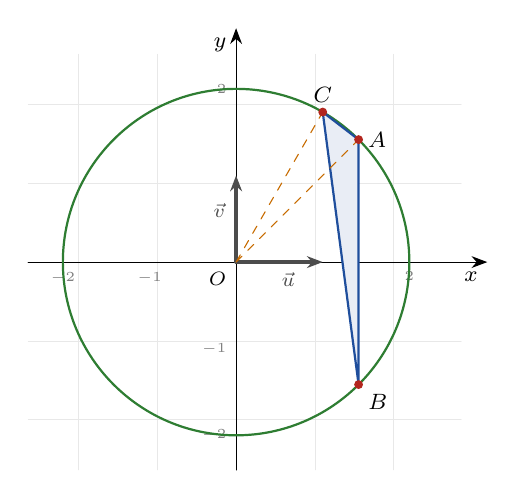
\begin{tikzpicture}[x=1.10cm,y=1.10cm,font=\footnotesize,line cap=round]
\draw[gray!18,very thin] (-2.4,-2.4) grid (2.6,2.4);
\draw[-{Stealth[length=2mm]}] (-2.4,0)--(2.9,0) node[below left]{$x$};
\draw[-{Stealth[length=2mm]}] (0,-2.4)--(0,2.7) node[below left]{$y$};
\node[below left,font=\scriptsize] at (0,0){$O$};
\draw[-{Stealth[length=2mm]},very thick,black!70] (0,0)--(1,0) node[pos=.6,below,font=\scriptsize]{$\vec u$};
\draw[-{Stealth[length=2mm]},very thick,black!70] (0,0)--(0,1) node[pos=.6,left,font=\scriptsize]{$\vec v$};
\node[below,font=\tiny,gray] at (-2,0){$-2$};
\node[below,font=\tiny,gray] at (-1,0){$-1$};
\node[below,font=\tiny,gray] at (2,0){$2$};
\node[left,font=\tiny,gray] at (0,-2){$-2$};
\node[left,font=\tiny,gray] at (0,-1){$-1$};
\node[left,font=\tiny,gray] at (0,2){$2$};
\begin{scope}\clip (-2.4,-2.4) rectangle (2.8,2.6);
\draw[cRem,thick] (0,0) circle (2);\fill[cDef!10] (1.4142,1.4142)--(1.4142,-1.4142)--(1.0000,1.7321)--cycle;\draw[cDef,thick] (1.4142,1.4142)--(1.4142,-1.4142)--(1.0000,1.7321)--cycle;\draw[cEx,dashed] (0,0)--(1.4142,1.4142) (0,0)--(1,1.7321);
\end{scope}
\fill[cThm] (1.4142,1.4142) circle (1.6pt) node[right,text=black]{$A$};
\fill[cThm] (1.4142,-1.4142) circle (1.6pt) node[below right,text=black]{$B$};
\fill[cThm] (1.0000,1.7321) circle (1.6pt) node[above,text=black]{$C$};
\end{tikzpicture}\end{LTR}\end{center}
\QQ{3}\pa $|K|=\dfrac{|z_C|}{2|z_A|}=\dfrac{2}{4}=\bx{\dfrac12}$ و$\arg K=\arg z_C-\arg z_A=\dfrac{\pi}{3}-\dfrac{\pi}{4}=\bx{\dfrac{\pi}{12}}$ (بترديد $2\pi$).

الشكل الجبري:
\[K=\frac{1+i\sqrt3}{2\sqrt2(1+i)}=\frac{(1+i\sqrt3)(1-i)}{2\sqrt2\times2}=\frac{\left(1+\sqrt3\right)+i\left(\sqrt3-1\right)}{4\sqrt2}=\bx{\frac{\sqrt6+\sqrt2}{8}+i\,\frac{\sqrt6-\sqrt2}{8}}\]
\pb $K=\frac12\left(\cos\frac{\pi}{12}+i\sin\frac{\pi}{12}\right)$، وبالمطابقة:
\[\bx{\cos\frac{\pi}{12}=\frac{\sqrt6+\sqrt2}{4}}\qquad\bx{\sin\frac{\pi}{12}=\frac{\sqrt6-\sqrt2}{4}}\]
\QQ{4} $z_B=\overline{z_A}$، ومنه $z_B^{\,n}=\left(\overline{z_A}\right)^n=\overline{z_A^{\,n}}$، إذن:
\[L_n=z_A^{\,n}+\overline{z_A^{\,n}}=2\operatorname{Re}\left(z_A^{\,n}\right)=2\times2^n\cos\frac{n\pi}{4}=\bx{2^{n+1}\cos\frac{n\pi}{4}\in\mathbb{R}}\]
(لأن $z+\overline{z}=2\operatorname{Re}(z)$ عدد حقيقي، وحسب دستور موافر $z_A^{\,n}=2^n\left(\cos\frac{n\pi}{4}+i\sin\frac{n\pi}{4}\right)$.)
\end{hal}

% ===================== التمرين 8 =====================
\begin{tamrin}{بكالوريا 2019 -- الموضوع الأول -- شعبة رياضيات}
في المستوي المركب المنسوب إلى المعلم المتعامد والمتجانس $\left(O;\vec u,\vec v\right)$، نعتبر النقط $A$، $B$، $C$، $D$ و$E$ حيث:
\[z_A=1+i\sqrt2,\quad z_B=i,\quad z_C=\overline{z_A},\quad z_D=\overline{z_B},\quad z_E=1.\]
\QQ{1} حل في المجموعة $\mathbb{C}$ المعادلة ذات المجهول $z$: $\left(z^2+1\right)\left(z^2-2z+3\right)=0$.

\QQ{2}
\begin{sq}
\qa أحسب كلا من $\left|z_A-1\right|$، $\left|z_B-1\right|$ و$\left|z_C-z_E\right|$ ثم تحقق أن النقط الأربعة $A$، $B$، $C$ و$D$ تنتمي إلى نفس الدائرة التي يطلب تعيين مركزها وطول نصف قطرها.
\qb بين أن: $z_B-z_E=\dfrac{\sqrt2}{2}(1+i)\left(z_A-z_E\right)$، ثم استنتج أن $B$ هي صورة $A$ بتحويل نقطي يطلب تعيين عناصره المميزة. ما طبيعة المثلث $ABE$؟
\end{sq}
\QQ{3} عين لاحقتي الشعاعين $\overrightarrow{BD}$ و$\overrightarrow{AE}$ محددا طبيعة الرباعي $ABDE$.

\QQ{4} $\vec w_1$ و$\vec w_2$ شعاعان من المستوي لاحقتاهما على الترتيب $z_1$ و$z_2$.
\begin{sq}
\qa برهن أن: ($\vec w_1$ و$\vec w_2$ متعامدان) يكافئ ($z_1\overline{z_2}+\overline{z_1}z_2=0$).
\qb عين مجموعة النقط $M$ من المستوي ذات اللاحقة $z$ حيث: $\left(z-z_A\right)\left(\overline{z}-z_D\right)+\left(z-z_B\right)\left(\overline{z}-z_C\right)=0$.
\end{sq}
\end{tamrin}
\begin{hal}
\QQ{1} $z^2+1=0\iff z=i$ أو $z=-i$.\quad $z^2-2z+3=0$: $\Delta=4-12=-8=\left(2i\sqrt2\right)^2$، ومنه $z=1\pm i\sqrt2$.
\[\bx{S=\left\{-i\,;\,i\,;\,1-i\sqrt2\,;\,1+i\sqrt2\right\}}\]
\QQ{2}\pa $z_C=1-i\sqrt2$ و$z_D=-i$.
\[\left|z_A-1\right|=\left|i\sqrt2\right|=\sqrt2,\quad \left|z_B-1\right|=\left|-1+i\right|=\sqrt2,\quad \left|z_C-z_E\right|=\left|-i\sqrt2\right|=\sqrt2\]
وكذلك $\left|z_D-z_E\right|=\left|-1-i\right|=\sqrt2$. إذن $EA=EB=EC=ED=\sqrt2$:\par
\bxt{النقط $A$، $B$، $C$ و$D$ تنتمي إلى الدائرة التي مركزها $E$ ونصف قطرها $\sqrt2$}.

\pb $\dfrac{\sqrt2}{2}(1+i)\left(z_A-z_E\right)=\dfrac{\sqrt2}{2}(1+i)\left(i\sqrt2\right)=i(1+i)=-1+i=z_B-z_E$. \ok

و$\frac{\sqrt2}{2}(1+i)=\cos\frac{\pi}{4}+i\sin\frac{\pi}{4}=e^{i\frac{\pi}{4}}$، فالعلاقة من الشكل $z_B-z_E=e^{i\frac{\pi}{4}}\left(z_A-z_E\right)$، إذن:\par
\bxt{$B$ صورة $A$ بالدوران الذي مركزه $E$ وزاويته $\frac{\pi}{4}$}.

ومنه $EA=EB$ و$\left(\overrightarrow{EA};\overrightarrow{EB}\right)=\frac{\pi}{4}+2k\pi$: \bxt{المثلث $ABE$ متساوي الساقين رأسه $E$}.

\QQ{3} $z_{\overrightarrow{BD}}=z_D-z_B=-i-i=\bx{-2i}$ و$z_{\overrightarrow{AE}}=z_E-z_A=\bx{-i\sqrt2}$.

$z_{\overrightarrow{BD}}=\sqrt2\,z_{\overrightarrow{AE}}$، إذن $\overrightarrow{BD}=\sqrt2\,\overrightarrow{AE}$: المستقيمان $(BD)$ و$(AE)$ متوازيان و$BD\neq AE$.
والضلعان الآخران $(AB)$ و$(DE)$ غير متوازيين (لأن $z_B-z_A=-1+i\left(1-\sqrt2\right)$ و$z_E-z_D=1+i$ غير مرتبطين خطيا). إذن \bxt{الرباعي $ABDE$ شبه منحرف قاعدتاه $[BD]$ و$[AE]$}.
\begin{center}\begin{LTR}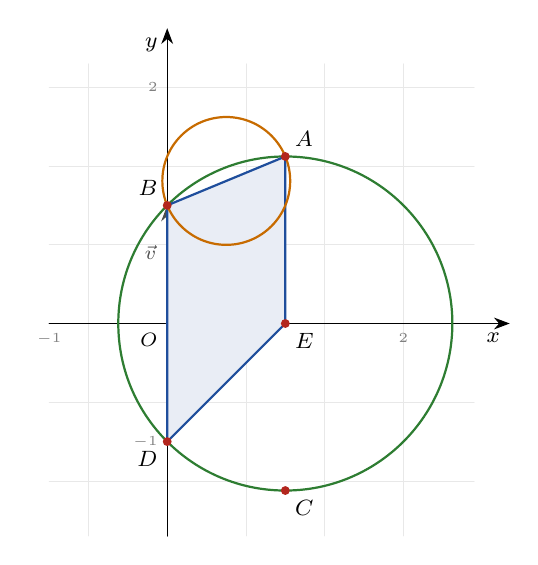
\begin{tikzpicture}[x=1.50cm,y=1.50cm,font=\footnotesize,line cap=round]
\draw[gray!18,very thin] (-1,-1.8) grid (2.6,2.2);
\draw[-{Stealth[length=2mm]}] (-1,0)--(2.9,0) node[below left]{$x$};
\draw[-{Stealth[length=2mm]}] (0,-1.8)--(0,2.5) node[below left]{$y$};
\node[below left,font=\scriptsize] at (0,0){$O$};
\draw[-{Stealth[length=2mm]},very thick,black!70] (0,0)--(1,0) node[pos=.6,below,font=\scriptsize]{$\vec u$};
\draw[-{Stealth[length=2mm]},very thick,black!70] (0,0)--(0,1) node[pos=.6,left,font=\scriptsize]{$\vec v$};
\node[below,font=\tiny,gray] at (-1,0){$-1$};
\node[below,font=\tiny,gray] at (2,0){$2$};
\node[left,font=\tiny,gray] at (0,-1){$-1$};
\node[left,font=\tiny,gray] at (0,2){$2$};
\begin{scope}\clip (-1,-1.8) rectangle (2.8,2.4);
\draw[cRem,thick] (1,0) circle (1.4142);\fill[cDef!10] (1.0000,1.4142)--(0.0000,1.0000)--(0.0000,-1.0000)--(1.0000,0.0000)--cycle;\draw[cDef,thick] (1.0000,1.4142)--(0.0000,1.0000)--(0.0000,-1.0000)--(1.0000,0.0000)--cycle;\draw[cEx,thick] (.5,1.2071) circle (0.5412);
\end{scope}
\fill[cThm] (1.0000,1.4142) circle (1.6pt) node[above right,text=black]{$A$};
\fill[cThm] (0.0000,1.0000) circle (1.6pt) node[above left,text=black]{$B$};
\fill[cThm] (1.0000,-1.4142) circle (1.6pt) node[below right,text=black]{$C$};
\fill[cThm] (0.0000,-1.0000) circle (1.6pt) node[below left,text=black]{$D$};
\fill[cThm] (1.0000,0.0000) circle (1.6pt) node[below right,text=black]{$E$};
\end{tikzpicture}\end{LTR}\end{center}
\QQ{4}\pa نضع $z_1=x_1+iy_1$ و$z_2=x_2+iy_2$. لدينا $z_1\overline{z_2}+\overline{z_1}z_2=z_1\overline{z_2}+\overline{z_1\overline{z_2}}=2\operatorname{Re}\left(z_1\overline{z_2}\right)$، و
\[z_1\overline{z_2}=(x_1+iy_1)(x_2-iy_2)=\left(x_1x_2+y_1y_2\right)+i\left(y_1x_2-x_1y_2\right).\]
إذن $z_1\overline{z_2}+\overline{z_1}z_2=2\left(x_1x_2+y_1y_2\right)=2\,\vec w_1\cdot\vec w_2$، ومنه:
\[\vec w_1\perp\vec w_2\iff \vec w_1\cdot\vec w_2=0\iff z_1\overline{z_2}+\overline{z_1}z_2=0.\]
\pb لدينا $z_D=\overline{z_B}$ و$z_C=\overline{z_A}$، إذن $\overline{z}-z_D=\overline{z-z_B}$ و$\overline{z}-z_C=\overline{z-z_A}$، فتصبح المعادلة:
\[\left(z-z_A\right)\overline{\left(z-z_B\right)}+\overline{\left(z-z_A\right)}\left(z-z_B\right)=0.\]
نضع $z_1=z-z_A$ (لاحقة $\overrightarrow{AM}$) و$z_2=z-z_B$ (لاحقة $\overrightarrow{BM}$)، فحسب السؤال (أ): $\overrightarrow{AM}\cdot\overrightarrow{BM}=0$.

إذن المجموعة هي \bxt{الدائرة ذات القطر $[AB]$}، مركزها منتصف $[AB]$ ذو اللاحقة $\bx{\frac12+i\,\frac{1+\sqrt2}{2}}$ ونصف قطرها
$\frac{AB}{2}=\frac{\left|-1+i\left(1-\sqrt2\right)\right|}{2}=\bx{\frac{\sqrt{4-2\sqrt2}}{2}}$ (الدائرة البرتقالية في الشكل).
\end{hal}

% ===================== التمرين 9 =====================
\begin{tamrin}{بكالوريا 2019 -- الموضوع الثاني -- شعبة رياضيات}
\QQ{1} نضع من أجل كل عدد مركب $z$: $P(z)=z^4-6z^3+29z^2-24z+100$.
\begin{sq}
\qa بين أنه من أجل كل عدد مركب $z$: $\overline{P(z)}=P\left(\overline{z}\right)$، ثم استنتج أنه إذا كان $z$ حلا للمعادلة $P(z)=0$ فإن $\overline{z}$ حل لها.
\qb حل في مجموعة الأعداد المركبة $\mathbb{C}$ المعادلة $P(z)=0$ علما أنها تقبل حلا تخيليا صرفا.
\end{sq}
\QQ{2} نعتبر في المستوي المركب المنسوب إلى المعلم المتعامد والمتجانس $\left(O;\vec u,\vec v\right)$ النقط $A$، $B$، $M$ و$M'$ التي لاحقاتها على الترتيب: $2i$، $3-4i$، $z$ و$z'$ حيث: $z'=\dfrac{-iz+4+3i}{z-2i}$ مع $z\neq2i$.
ولتكن $I$ مرجح الجملة $\left\{(A;2),(B;1)\right\}$ و$J$ مرجح الجملة $\left\{(A;-2),(B;1)\right\}$.
\begin{sq}
\qa عين اللاحقتين $z_I$ و$z_J$ للنقطتين $I$ و$J$ على الترتيب.
\qb لتكن $(E)$ مجموعة النقط $M(z)$ التي يكون من أجلها $|z'|=2$.

بين أن ($M$ من $(E)$) يكافئ ($\overrightarrow{IM}\cdot\overrightarrow{JM}=0$)، ثم عين $(E)$ وأنشئها.
\qc لتكن $(\Gamma)$ مجموعة النقط $M(z)$ التي يكون من أجلها $\arg\left(z'\right)=2k\pi$ حيث $k$ عدد صحيح.

تحقق أن النقطة $D$ ذات اللاحقة $\dfrac92-\dfrac52i$ تنتمي إلى $(\Gamma)$، ثم عين وأنشئ $(\Gamma)$.
\end{sq}
\QQ{3} عين الشكل الجبري للاحقة النقطة $G$ تقاطع المجموعتين $(E)$ و$(\Gamma)$.
\end{tamrin}
\begin{hal}
\QQ{1}\pa معاملات $P$ حقيقية، ومرافق مجموع (جداء) هو مجموع (جداء) المرافقات، و$\overline{a}=a$ لكل حقيقي $a$:
\[\overline{P(z)}=\overline{z}^{\,4}-6\overline{z}^{\,3}+29\overline{z}^{\,2}-24\overline{z}+100=P\left(\overline{z}\right).\]
إذا كان $P(z)=0$ فإن $P\left(\overline{z}\right)=\overline{P(z)}=\overline{0}=0$، أي $\overline{z}$ حل أيضا.

\pb نبحث عن حل $z=iy$ ($y\in\mathbb{R}^*$): $P(iy)=y^4-6i^3y^3-29y^2-24iy+100=\left(y^4-29y^2+100\right)+i\left(6y^3-24y\right)$.
\[P(iy)=0\iff\begin{cases}y^4-29y^2+100=0\\ 6y\left(y^2-4\right)=0\end{cases}\]
المعادلة الثانية تعطي $y=2$ أو $y=-2$ ($y\neq0$)، وتحقق الأولى: $16-116+100=0$. إذن $2i$ حل، و$-2i=\overline{2i}$ حل حسب (أ)،
ومنه $P(z)$ يقبل القسمة على $(z-2i)(z+2i)=z^2+4$. بالقسمة الإقليدية (أو المطابقة):
\[P(z)=\left(z^2+4\right)\left(z^2-6z+25\right).\]
$z^2-6z+25=0$: $\Delta=36-100=-64=(8i)^2$، ومنه $z=3\pm4i$.
\[\bx{S=\left\{-2i\,;\,2i\,;\,3-4i\,;\,3+4i\right\}}\]
\QQ{2}\pa $z_I=\dfrac{2z_A+z_B}{3}=\dfrac{4i+3-4i}{3}=\bx{1}$،\quad $z_J=\dfrac{-2z_A+z_B}{-2+1}=\dfrac{-4i+3-4i}{-1}=\bx{-3+8i}$.

\pb نلاحظ أن $-iz+4+3i=-i\left(z-3+4i\right)=-i\left(z-z_B\right)$، إذن $z'=-i\,\dfrac{z-z_B}{z-z_A}$، ومنه $|z'|=\dfrac{MB}{MA}$.
\begin{align*}M\in(E)&\iff MB=2MA\iff MB^2-4MA^2=0\\&\iff\left(\overrightarrow{MB}-2\overrightarrow{MA}\right)\cdot\left(\overrightarrow{MB}+2\overrightarrow{MA}\right)=0.\end{align*}
حسب خاصية المرجح: $2\overrightarrow{MA}+\overrightarrow{MB}=3\overrightarrow{MI}$ و$-2\overrightarrow{MA}+\overrightarrow{MB}=-\overrightarrow{MJ}$، إذن:
\[M\in(E)\iff-3\,\overrightarrow{MI}\cdot\overrightarrow{MJ}=0\iff\overrightarrow{IM}\cdot\overrightarrow{JM}=0.\]
($A\notin(E)$ لأن $AB\neq0$.) إذن \bxt{$(E)$ هي الدائرة ذات القطر $[IJ]$}: مركزها $\Omega$ منتصف $[IJ]$: $z_\Omega=\bx{-1+4i}$، ونصف قطرها $\dfrac{IJ}{2}=\dfrac{|-4+8i|}{2}=\bx{2\sqrt5}$.

\pc من أجل $D$: $z_D-z_B=\frac32+\frac32i$ و$z_D-z_A=\frac92-\frac92i$، ومنه
$z'_D=-i\cdot\dfrac{\frac32(1+i)}{\frac92(1-i)}=-i\cdot\dfrac13\cdot i=\dfrac13>0$، إذن $\arg z'_D=0$ أي $D\in(\Gamma)$. \ok

بصفة عامة ($M\neq A$ و$M\neq B$): $\arg z'=\arg(-i)+\arg\dfrac{z-z_B}{z-z_A}=-\dfrac{\pi}{2}+\left(\overrightarrow{MA};\overrightarrow{MB}\right)$، إذن:
\[M\in(\Gamma)\iff\left(\overrightarrow{MA};\overrightarrow{MB}\right)=\frac{\pi}{2}+2k\pi.\]
فالنقطة $M$ ترى $[AB]$ بزاوية قائمة موجهة في الاتجاه المباشر، إذن \bxt{$(\Gamma)$ نصف الدائرة ذات القطر $[AB]$ الواقع في جهة $D$، باستثناء $A$ و$B$}،
مركزها منتصف $[AB]$ ذو اللاحقة $\frac32-i$ ونصف قطرها $\frac{|3-6i|}{2}=\frac{3\sqrt5}{2}$.

\QQ{3} نضع $z=x+iy$. معادلة $(E)$: $(x+1)^2+(y-4)^2=20$، أي $x^2+y^2+2x-8y-3=0$.
معادلة الدائرة ذات القطر $[AB]$: $\left(x-\frac32\right)^2+(y+1)^2=\frac{45}{4}$، أي $x^2+y^2-3x+2y-8=0$.
بالطرح: $5x-10y+5=0$ أي $x=2y-1$. بالتعويض في الثانية: $(2y-1)^2+y^2-3(2y-1)+2y-8=0$، أي $5y^2-8y-4=0$،
ومنه $y=2$ ($x=3$) أو $y=-\frac25$ ($x=-\frac95$).

$z=3+2i$: $z'=\dfrac{-i(3+2i)+4+3i}{3+2i-2i}=\dfrac{6}{3}=2>0$ \ok.

$z=-\frac95-\frac25i$: $z'=\dfrac{-i\left(-\frac95-\frac25i\right)+4+3i}{-\frac95-\frac{12}{5}i}=\dfrac{\frac{18}{5}+\frac{24}{5}i}{-\frac95-\frac{12}{5}i}=-2<0$، فهذه النقطة لا تنتمي إلى $(\Gamma)$.

إذن: \bx{z_G=3+2i}
\begin{center}\begin{LTR}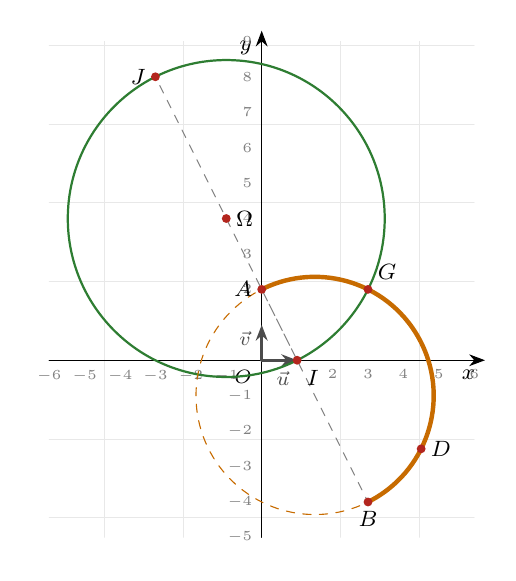
\begin{tikzpicture}[x=0.45cm,y=0.45cm,font=\footnotesize,line cap=round]
\draw[gray!18,very thin] (-6,-5) grid (6,9);
\draw[-{Stealth[length=2mm]}] (-6,0)--(6.3,0) node[below left]{$x$};
\draw[-{Stealth[length=2mm]}] (0,-5)--(0,9.3) node[below left]{$y$};
\node[below left,font=\scriptsize] at (0,0){$O$};
\draw[-{Stealth[length=2mm]},very thick,black!70] (0,0)--(1,0) node[pos=.6,below,font=\scriptsize]{$\vec u$};
\draw[-{Stealth[length=2mm]},very thick,black!70] (0,0)--(0,1) node[pos=.6,left,font=\scriptsize]{$\vec v$};
\node[below,font=\tiny,gray] at (-6,0){$-6$};
\node[below,font=\tiny,gray] at (-5,0){$-5$};
\node[below,font=\tiny,gray] at (-4,0){$-4$};
\node[below,font=\tiny,gray] at (-3,0){$-3$};
\node[below,font=\tiny,gray] at (-2,0){$-2$};
\node[below,font=\tiny,gray] at (-1,0){$-1$};
\node[below,font=\tiny,gray] at (2,0){$2$};
\node[below,font=\tiny,gray] at (3,0){$3$};
\node[below,font=\tiny,gray] at (4,0){$4$};
\node[below,font=\tiny,gray] at (5,0){$5$};
\node[below,font=\tiny,gray] at (6,0){$6$};
\node[left,font=\tiny,gray] at (0,-5){$-5$};
\node[left,font=\tiny,gray] at (0,-4){$-4$};
\node[left,font=\tiny,gray] at (0,-3){$-3$};
\node[left,font=\tiny,gray] at (0,-2){$-2$};
\node[left,font=\tiny,gray] at (0,-1){$-1$};
\node[left,font=\tiny,gray] at (0,2){$2$};
\node[left,font=\tiny,gray] at (0,3){$3$};
\node[left,font=\tiny,gray] at (0,4){$4$};
\node[left,font=\tiny,gray] at (0,5){$5$};
\node[left,font=\tiny,gray] at (0,6){$6$};
\node[left,font=\tiny,gray] at (0,7){$7$};
\node[left,font=\tiny,gray] at (0,8){$8$};
\node[left,font=\tiny,gray] at (0,9){$9$};
\begin{scope}\clip (-6,-5) rectangle (6.2,9.2);
\draw[cRem,thick] (-1,4) circle (4.4721);\draw[cEx,dashed] (1.5,-1) circle (3.3541);\draw[cEx,line width=1.6pt] ([shift={(-63.435:3.3541)}]1.5,-1) arc (-63.435:116.565:3.3541);\draw[gray,dashed] (1,0)--(-3,8) (0,2)--(3,-4);
\end{scope}
\fill[cThm] (0.0000,2.0000) circle (1.6pt) node[left,text=black]{$A$};
\fill[cThm] (3.0000,-4.0000) circle (1.6pt) node[below,text=black]{$B$};
\fill[cThm] (1.0000,0.0000) circle (1.6pt) node[below right,text=black]{$I$};
\fill[cThm] (-3.0000,8.0000) circle (1.6pt) node[left,text=black]{$J$};
\fill[cThm] (4.5000,-2.5000) circle (1.6pt) node[right,text=black]{$D$};
\fill[cThm] (3.0000,2.0000) circle (1.6pt) node[above right,text=black]{$G$};
\fill[cThm] (-1.0000,4.0000) circle (1.6pt) node[right,text=black]{$\Omega$};
\end{tikzpicture}\end{LTR}\end{center}
\end{hal}

% ===================== التمرين 10 =====================
\begin{tamrin}{بكالوريا 2018 -- الموضوع الأول -- شعبة رياضيات}
المستوي منسوب إلى المعلم المتعامد والمتجانس $\left(O;\vec u,\vec v\right)$، $\theta$ عدد حقيقي من المجال $\left]-\pi;\pi\right]$.

\textbf{I)} حل في $\mathbb{C}$ المعادلة ذات المجهول $z$: $\left(z^2-2z+2\right)\left(z^2-2(\sin\theta)z+1\right)=0$.

\textbf{II)} $A$، $B$، $C$ و$D$ نقط من المستوي لاحقاتها على الترتيب:
$z_A=-\sqrt2\,e^{i\frac{5\pi}{4}}$، $z_B=1-i$، $z_C=\sin\theta+i\cos\theta$ و$z_D=\overline{z_C}$ ($\overline{z_C}$ يرمز إلى مرافق $z_C$).

\QQ{1} أكتب الأعداد $z_A$، $z_B$، $z_C$ و$z_D=\overline{z_C}$ على الشكل الأسي.

\QQ{2} $E$ نقطة من المستوي لاحقتها $z_E$ حيث: $z_E=\dfrac{z_A}{z_B}$. بين أن النقط $C$، $D$ و$E$ تنتمي إلى دائرة واحدة يطلب تعيين مركزها ونصف قطرها.

\QQ{3} ليكن $S$ التشابه المباشر الذي مركزه النقطة $A$ وزاويته $\dfrac{\pi}{4}$ ونسبته $\left(2\sqrt2-2\right)$.
عين قيمة $\theta$ حتى تكون النقطة $B$ صورة النقطة $C$ بالتشابه المباشر $S$.

\QQ{4} نضع: $\theta=-\dfrac{3\pi}{4}$. عين قيم العدد الطبيعي $n$ والتي من أجلها يكون العدد $\left(z_D\right)^n$ تخيليا صرفا.
\end{tamrin}
\begin{hal}
\textbf{I)} $z^2-2z+2=0$: $\Delta=-4=(2i)^2$، ومنه $z=1+i$ أو $z=1-i$.

$z^2-2(\sin\theta)z+1=0$: $\Delta'=\sin^2\theta-1=-\cos^2\theta=(i\cos\theta)^2$، ومنه $z=\sin\theta+i\cos\theta$ أو $z=\sin\theta-i\cos\theta$ (حل مضاعف $\sin\theta$ إذا كان $\cos\theta=0$).
\[\bx{S=\left\{1+i\,;\,1-i\,;\,\sin\theta+i\cos\theta\,;\,\sin\theta-i\cos\theta\right\}}\]
\textbf{II)}\QQ{1} $-1=e^{i\pi}$، إذن $z_A=\sqrt2\,e^{i\pi}e^{i\frac{5\pi}{4}}=\sqrt2\,e^{i\frac{9\pi}{4}}$: \bx{z_A=\sqrt2\,e^{i\frac{\pi}{4}}} (أي $z_A=1+i$).\quad
\bx{z_B=\sqrt2\,e^{-i\frac{\pi}{4}}}

$z_C=\cos\left(\frac{\pi}{2}-\theta\right)+i\sin\left(\frac{\pi}{2}-\theta\right)$: \bx{z_C=e^{i\left(\frac{\pi}{2}-\theta\right)}}،\quad \bx{z_D=\overline{z_C}=e^{i\left(\theta-\frac{\pi}{2}\right)}}

\QQ{2} $z_E=\dfrac{\sqrt2\,e^{i\frac{\pi}{4}}}{\sqrt2\,e^{-i\frac{\pi}{4}}}=e^{i\frac{\pi}{2}}=i$. إذن $|z_C|=|z_D|=|z_E|=1$، أي $OC=OD=OE=1$:\par
\bxt{$C$، $D$ و$E$ تنتمي إلى الدائرة التي مركزها $O$ ونصف قطرها $1$}.

\QQ{3} العبارة المركبة لـ $S$: $z'-z_A=\left(2\sqrt2-2\right)e^{i\frac{\pi}{4}}\left(z-z_A\right)$. لدينا $\left(2\sqrt2-2\right)e^{i\frac{\pi}{4}}=\left(2\sqrt2-2\right)\frac{\sqrt2}{2}(1+i)=\left(2-\sqrt2\right)(1+i)$.
\begin{align*}S(C)=B&\iff z_C-z_A=\frac{z_B-z_A}{\left(2-\sqrt2\right)(1+i)}=\frac{-2i}{\left(2-\sqrt2\right)(1+i)}\\&\iff z_C-z_A=\frac{-2i(1-i)}{2\left(2-\sqrt2\right)}=\frac{-1-i}{2-\sqrt2}=-\frac{2+\sqrt2}{2}(1+i).\end{align*}
ومنه $z_C=(1+i)\left(1-\frac{2+\sqrt2}{2}\right)=-\frac{\sqrt2}{2}-\frac{\sqrt2}{2}i=e^{-i\frac{3\pi}{4}}$.
إذن $\frac{\pi}{2}-\theta=-\frac{3\pi}{4}+2k\pi$، أي $\theta=\frac{5\pi}{4}-2k\pi$، ومع $\theta\in\left]-\pi;\pi\right]$: \bx{\theta=-\frac{3\pi}{4}}

\QQ{4} $\theta=-\frac{3\pi}{4}$: $z_D=e^{i\left(-\frac{3\pi}{4}-\frac{\pi}{2}\right)}=e^{-i\frac{5\pi}{4}}=e^{i\frac{3\pi}{4}}$، ومنه $\left(z_D\right)^n=e^{i\frac{3n\pi}{4}}$.
يكون $\left(z_D\right)^n$ تخيليا صرفا إذا وفقط إذا كان $\cos\frac{3n\pi}{4}=0$:
\[\cos\frac{3n\pi}{4}=0\iff\frac{3n\pi}{4}=\frac{\pi}{2}+k\pi\iff3n=2+4k\ \ (k\in\mathbb{Z}).\]
أي $3n\equiv2\,[4]$؛ وبما أن $3\times3\equiv1\,[4]$ نضرب في $3$: $n\equiv6\equiv2\,[4]$. إذن \bx{n=4k+2,\ \ k\in\mathbb{N}}
\begin{center}\begin{LTR}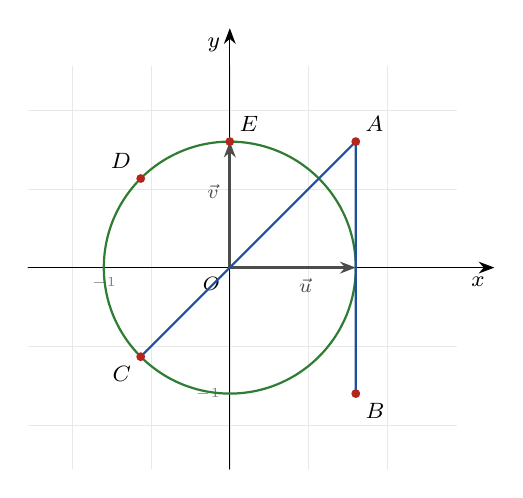
\begin{tikzpicture}[x=1.60cm,y=1.60cm,font=\footnotesize,line cap=round]
\draw[gray!18,very thin] (-1.6,-1.6) grid (1.8,1.6);
\draw[-{Stealth[length=2mm]}] (-1.6,0)--(2.1,0) node[below left]{$x$};
\draw[-{Stealth[length=2mm]}] (0,-1.6)--(0,1.9) node[below left]{$y$};
\node[below left,font=\scriptsize] at (0,0){$O$};
\draw[-{Stealth[length=2mm]},very thick,black!70] (0,0)--(1,0) node[pos=.6,below,font=\scriptsize]{$\vec u$};
\draw[-{Stealth[length=2mm]},very thick,black!70] (0,0)--(0,1) node[pos=.6,left,font=\scriptsize]{$\vec v$};
\node[below,font=\tiny,gray] at (-1,0){$-1$};
\node[left,font=\tiny,gray] at (0,-1){$-1$};
\begin{scope}\clip (-1.6,-1.6) rectangle (2,1.8);
\draw[cRem,thick] (0,0) circle (1);\draw[cDef,thick] (1,1)--(-.7071,-.7071) (1,1)--(1,-1);
\end{scope}
\fill[cThm] (1.0000,1.0000) circle (1.6pt) node[above right,text=black]{$A$};
\fill[cThm] (1.0000,-1.0000) circle (1.6pt) node[below right,text=black]{$B$};
\fill[cThm] (-0.7071,-0.7071) circle (1.6pt) node[below left,text=black]{$C$};
\fill[cThm] (-0.7071,0.7071) circle (1.6pt) node[above left,text=black]{$D$};
\fill[cThm] (0.0000,1.0000) circle (1.6pt) node[above right,text=black]{$E$};
\end{tikzpicture}\end{LTR}\end{center}
\end{hal}

% ===================== التمرين 11 =====================
\begin{tamrin}{بكالوريا 2018 -- الموضوع الثاني -- شعبة رياضيات}
\QQ{1} $m$ عدد حقيقي. نعتبر في $\mathbb{C}$ المعادلة $(E)$ التالية: $z^2+(m+1)z+(2m-1)=0$.
عين قيم العدد الحقيقي $m$ التي من أجلها تقبل المعادلة $(E)$ حلين مركبين غير حقيقيين.

\QQ{2} نضع: $m=3$. حل المعادلة $(E)$.

\QQ{3} نعتبر في المستوي المركب المنسوب إلى المعلم المتعامد والمتجانس $\left(O;\vec u,\vec v\right)$ النقط $A$، $B$، $C$ و$E$ التي لاحقاتها:
$z_A=-2+i$، $z_B=-2-i$، $z_C=\alpha$ و$z_E=\sqrt3$ حيث $\alpha$ عدد حقيقي و$\alpha>-2$.
بين أن قيمة $\alpha$ التي من أجلها يكون المثلث $ABC$ متقايس الأضلاع هي $\left(-2+\sqrt3\right)$.
نضع في كل ما يأتي: $z_C=-2+\sqrt3$.

\QQ{4} أكتب العدد المركب $\dfrac{z_C-z_E}{z_A-z_B}$ على الشكل الأسي ثم استنتج أن:
\begin{sq}
\qa المستقيمين $(AB)$ و$(EC)$ متعامدان.
\qb النقط $A$، $B$ و$E$ تنتمي إلى نفس الدائرة $(\gamma)$ وعين مركزها ونصف قطرها.
\end{sq}
\QQ{5} ليكن $r$ الدوران الذي يحول النقطة $B$ إلى $C$ ويحول $C$ إلى $A$، عبارته المركبة هي:
$z'=az+\left(\dfrac{\sqrt3-6}{2}\right)+i\left(\dfrac{2\sqrt3-1}{2}\right)$.
\begin{sq}
\qa أحسب العدد المركب $a$، ثم استنتج زاوية الدوران $r$.
\qb تحقق أن النقطة $G$ مركز ثقل المثلث $ABC$ هي مركز الدوران $r$.
\end{sq}
\end{tamrin}
\begin{hal}
\QQ{1} $\Delta=(m+1)^2-4(2m-1)=m^2-6m+5=(m-1)(m-5)$.
تقبل $(E)$ حلين مركبين غير حقيقيين $\iff\Delta<0\iff(m-1)(m-5)<0\iff$ \bx{1<m<5}

\QQ{2} $m=3$: $z^2+4z+5=0$، $\Delta=16-20=-4=(2i)^2$، ومنه \bx{S=\left\{-2-i\,;\,-2+i\right\}}

\QQ{3} $AB=|z_B-z_A|=|-2i|=2$، $CA=|-2+i-\alpha|=\sqrt{(\alpha+2)^2+1}$ و$CB=\sqrt{(\alpha+2)^2+1}$ (فدائما $CA=CB$).
المثلث $ABC$ متقايس الأضلاع إذا وفقط إذا كان $CA=AB$:
\[(\alpha+2)^2+1=4\iff(\alpha+2)^2=3\iff\alpha+2=\sqrt3\]
(لأن $\alpha+2>0$).
إذن \bx{\alpha=-2+\sqrt3}

\QQ{4} $z_C-z_E=-2+\sqrt3-\sqrt3=-2$ و$z_A-z_B=2i$، ومنه $\dfrac{z_C-z_E}{z_A-z_B}=\dfrac{-2}{2i}=i=\bx{e^{i\frac{\pi}{2}}}$

\pa $\left(\overrightarrow{BA};\overrightarrow{EC}\right)=\arg i=\frac{\pi}{2}+2k\pi$، إذن \bxt{$(AB)\perp(EC)$}.

\pb $\left|\frac{z_C-z_E}{z_A-z_B}\right|=1$ أي $EC=AB=2$، و$CA=CB=AB=2$ (المثلث متقايس الأضلاع). إذن $CA=CB=CE=2$:\par
\bxt{$A$، $B$ و$E$ تنتمي إلى الدائرة $(\gamma)$ التي مركزها $C$ ونصف قطرها $2$}.

\QQ{5}\pa $r(B)=C$ و$r(C)=A$: $z_C=az_B+b$ و$z_A=az_C+b$؛ بالطرح: $z_A-z_C=a\left(z_C-z_B\right)$:
\[a=\frac{z_A-z_C}{z_C-z_B}=\frac{-\sqrt3+i}{\sqrt3+i}=\frac{\left(-\sqrt3+i\right)\left(\sqrt3-i\right)}{4}=\frac{-2+2i\sqrt3}{4}=\bx{-\frac12+i\frac{\sqrt3}{2}=e^{i\frac{2\pi}{3}}}\]
إذن زاوية الدوران $r$ هي \bx{\frac{2\pi}{3}}

\pb $z_G=\dfrac{z_A+z_B+z_C}{3}=\dfrac{-6+\sqrt3}{3}=-2+\dfrac{\sqrt3}{3}$. نتحقق أن $r(G)=G$:
\begin{align*}az_G+b&=\left(-\tfrac12+i\tfrac{\sqrt3}{2}\right)\left(-2+\tfrac{\sqrt3}{3}\right)+\tfrac{\sqrt3-6}{2}+i\,\tfrac{2\sqrt3-1}{2}\\
&=\left(1-\tfrac{\sqrt3}{6}+\tfrac{\sqrt3}{2}-3\right)+i\left(-\sqrt3+\tfrac12+\sqrt3-\tfrac12\right)=-2+\tfrac{\sqrt3}{3}=z_G.\end{align*}
إذن $G$ صامدة بالدوران $r$ (الذي ليس التحويل المطابق)، فهي \bxt{مركز الدوران $r$}.
\begin{center}\begin{LTR}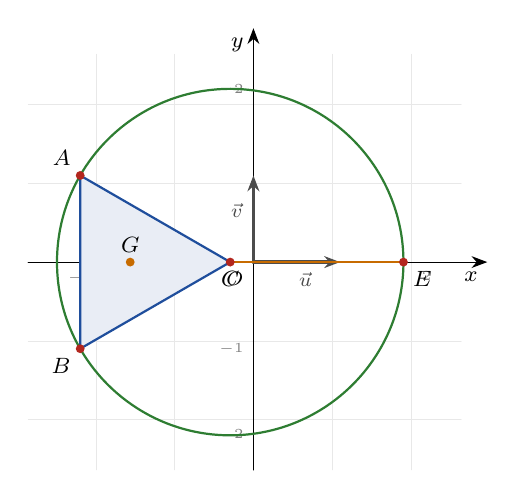
\begin{tikzpicture}[x=1.10cm,y=1.10cm,font=\footnotesize,line cap=round]
\draw[gray!18,very thin] (-2.6,-2.4) grid (2.4,2.4);
\draw[-{Stealth[length=2mm]}] (-2.6,0)--(2.7,0) node[below left]{$x$};
\draw[-{Stealth[length=2mm]}] (0,-2.4)--(0,2.7) node[below left]{$y$};
\node[below left,font=\scriptsize] at (0,0){$O$};
\draw[-{Stealth[length=2mm]},very thick,black!70] (0,0)--(1,0) node[pos=.6,below,font=\scriptsize]{$\vec u$};
\draw[-{Stealth[length=2mm]},very thick,black!70] (0,0)--(0,1) node[pos=.6,left,font=\scriptsize]{$\vec v$};
\node[below,font=\tiny,gray] at (-2,0){$-2$};
\node[below,font=\tiny,gray] at (-1,0){$-1$};
\node[below,font=\tiny,gray] at (2,0){$2$};
\node[left,font=\tiny,gray] at (0,-2){$-2$};
\node[left,font=\tiny,gray] at (0,-1){$-1$};
\node[left,font=\tiny,gray] at (0,2){$2$};
\begin{scope}\clip (-2.6,-2.4) rectangle (2.6,2.6);
\draw[cRem,thick] (-0.2679,0) circle (2);\fill[cDef!10] (-2.0000,1.0000)--(-2.0000,-1.0000)--(-0.2679,0.0000)--cycle;\draw[cDef,thick] (-2.0000,1.0000)--(-2.0000,-1.0000)--(-0.2679,0.0000)--cycle;\draw[cEx,thick] (-0.2679,0)--(1.7321,0);\fill[cEx] (-1.4226,0) circle (1.6pt) node[above,text=black]{$G$};
\end{scope}
\fill[cThm] (-2.0000,1.0000) circle (1.6pt) node[above left,text=black]{$A$};
\fill[cThm] (-2.0000,-1.0000) circle (1.6pt) node[below left,text=black]{$B$};
\fill[cThm] (-0.2679,0.0000) circle (1.6pt) node[below,text=black]{$C$};
\fill[cThm] (1.7321,0.0000) circle (1.6pt) node[below right,text=black]{$E$};
\end{tikzpicture}\end{LTR}\end{center}
\end{hal}

% ===================== التمرين 12 =====================
\begin{tamrin}{بكالوريا 2017 (الدورة الاستدراكية) -- الموضوع الأول -- شعبة رياضيات}
\textbf{I)} حل في مجموعة الأعداد المركبة $\mathbb{C}$ المعادلة ذات المجهول $z$: $2z^2-10z+\dfrac{29}{2}=0$.

\textbf{II)} المستوي المركب منسوب إلى المعلم المتعامد والمتجانس $\left(O;\vec u,\vec v\right)$.
نعتبر النقط $A$، $B$، $C$ و$D$ التي لاحقاتها: $z_A=\dfrac32+\sqrt2\,e^{i\frac{\pi}{4}}$، $z_B=\dfrac32\,e^{-i\frac{\pi}{2}}$، $z_C=-\overline{z_A}$ و$z_D=i$.

\QQ{1}
\begin{sq}
\qa أكتب كلا من $z_A$، $z_B$ و$z_C$ على الشكل الجبري، ثم علم $A$، $B$، $C$ و$D$ في المعلم السابق.
\qb أكتب العدد المركب $\dfrac{z_A-z_B}{z_C-z_B}$ على الشكل الأسي ثم استنتج طبيعة المثلث $ABC$.
\end{sq}
\QQ{2} جد لاحقة النقطة $E$ نظيرة $B$ بالنسبة للنقطة $D$، ثم استنتج طبيعة الرباعي $ABCE$.

\QQ{3} أكتب العبارة المركبة للتشابه $S$ الذي مركزه $B$ ويحول $A$ إلى $D$ ثم حدد نسبته وزاويته.

\begin{molahada}
حُذف السؤال 4 (متتالية النقط $A_{n+1}=S(A_n)$ والبرهان بالتراجع على لاحقة $A_n$ وانتماء $A_n$ إلى $(AB)$) لأنه خارج المنهاج الحالي (التوزيع السنوي 2026-2027): متتاليات النقط غير مدرجة في المنهاج.
\end{molahada}
\end{tamrin}
\begin{hal}
\textbf{I)} بضرب الطرفين في $2$: $4z^2-20z+29=0$، $\Delta=400-464=-64=(8i)^2$، ومنه $z=\dfrac{20\pm8i}{8}$:
\[\bx{S=\left\{\frac52-i\,;\,\frac52+i\right\}}\]
\textbf{II)}\QQ{1}\pa $\sqrt2\,e^{i\frac{\pi}{4}}=1+i$، إذن \bx{z_A=\frac52+i}،\quad $e^{-i\frac{\pi}{2}}=-i$: \bx{z_B=-\frac32i}،\quad \bx{z_C=-\left(\frac52-i\right)=-\frac52+i}
\pb $z_A-z_B=\frac52+\frac52i=\frac52(1+i)$ و$z_C-z_B=-\frac52+\frac52i=\frac52(-1+i)$:
\[\frac{z_A-z_B}{z_C-z_B}=\frac{1+i}{-1+i}=\frac{(1+i)(-1-i)}{2}=\frac{-2i}{2}=-i=\bx{e^{-i\frac{\pi}{2}}}\]
إذن $BA=BC$ و$\left(\overrightarrow{BC};\overrightarrow{BA}\right)=-\frac{\pi}{2}+2k\pi$: \bxt{المثلث $ABC$ قائم في $B$ ومتساوي الساقين}.

\QQ{2} $D$ منتصف $[BE]$: $z_E=2z_D-z_B=2i+\frac32i=\bx{\frac72i}$.

منتصف $[AC]$: $\frac{z_A+z_C}{2}=\frac{2i}{2}=i=z_D$؛ إذن القطران $[AC]$ و$[BE]$ متناصفان في $D$، فالرباعي $ABCE$ متوازي أضلاع، وفيه $BA=BC$ و$(BA)\perp(BC)$، إذن \bxt{الرباعي $ABCE$ مربع}.
\begin{center}\begin{LTR}\begin{tikzpicture}[x=0.90cm,y=0.90cm,font=\footnotesize,line cap=round]
\draw[gray!18,very thin] (-3,-2) grid (3.2,3.8);
\draw[-{Stealth[length=2mm]}] (-3,0)--(3.5,0) node[below left]{$x$};
\draw[-{Stealth[length=2mm]}] (0,-2)--(0,4.1) node[below left]{$y$};
\node[below left,font=\scriptsize] at (0,0){$O$};
\draw[-{Stealth[length=2mm]},very thick,black!70] (0,0)--(1,0) node[pos=.6,below,font=\scriptsize]{$\vec u$};
\draw[-{Stealth[length=2mm]},very thick,black!70] (0,0)--(0,1) node[pos=.6,left,font=\scriptsize]{$\vec v$};
\node[below,font=\tiny,gray] at (-3,0){$-3$};
\node[below,font=\tiny,gray] at (-2,0){$-2$};
\node[below,font=\tiny,gray] at (-1,0){$-1$};
\node[below,font=\tiny,gray] at (2,0){$2$};
\node[below,font=\tiny,gray] at (3,0){$3$};
\node[left,font=\tiny,gray] at (0,-2){$-2$};
\node[left,font=\tiny,gray] at (0,-1){$-1$};
\node[left,font=\tiny,gray] at (0,2){$2$};
\node[left,font=\tiny,gray] at (0,3){$3$};
\begin{scope}\clip (-3,-2) rectangle (3.4,4);
\fill[cDef!10] (2.5000,1.0000)--(0.0000,-1.5000)--(-2.5000,1.0000)--(0.0000,3.5000)--cycle;\draw[cDef,thick] (2.5000,1.0000)--(0.0000,-1.5000)--(-2.5000,1.0000)--(0.0000,3.5000)--cycle;\draw[black!70] (0.1556,-1.3444)--(0.0000,-1.1889)--(-0.1556,-1.3444);\draw[cEx,dashed] (2.5,1)--(-2.5,1) (0,-1.5)--(0,3.5);
\end{scope}
\fill[cThm] (2.5000,1.0000) circle (1.6pt) node[right,text=black]{$A$};
\fill[cThm] (0.0000,-1.5000) circle (1.6pt) node[below right,text=black]{$B$};
\fill[cThm] (-2.5000,1.0000) circle (1.6pt) node[left,text=black]{$C$};
\fill[cThm] (0.0000,1.0000) circle (1.6pt) node[above right,text=black]{$D$};
\fill[cThm] (0.0000,3.5000) circle (1.6pt) node[right,text=black]{$E$};
\end{tikzpicture}\end{LTR}\end{center}
\QQ{3} العبارة المركبة لتشابه مباشر مركزه $B$: $z'-z_B=k\left(z-z_B\right)$ حيث:
\[k=\frac{z_D-z_B}{z_A-z_B}=\frac{\frac52i}{\frac52(1+i)}=\frac{i(1-i)}{2}=\frac12+\frac12i.\]
\[z'=\left(\tfrac12+\tfrac12i\right)\left(z+\tfrac32i\right)-\tfrac32i=\bx{z'=\frac{1+i}{2}\,z-\frac34-\frac34i}\]
$\frac{1+i}{2}=\frac{\sqrt2}{2}e^{i\frac{\pi}{4}}$: نسبته \bx{\frac{\sqrt2}{2}} وزاويته \bx{\frac{\pi}{4}}

\end{hal}

% ===================== التمرين 13 =====================
\begin{tamrin}{بكالوريا 2017 (الدورة الاستدراكية) -- الموضوع الثاني -- شعبة رياضيات}
\textbf{I)} نعتبر في مجموعة الأعداد المركبة $\mathbb{C}$ المعادلة $(E)$: $z^2-2(1-\sin\alpha)z+2(1-\sin\alpha)=0$، حيث $\alpha$ عدد حقيقي.
(نرمز بـ $z_1$ و$z_2$ إلى حلي المعادلة $(E)$.)

\QQ{1} عين الحلين $z_1$ و$z_2$ بدلالة $\alpha$.

\QQ{2} نضع: $\alpha=\dfrac{\pi}{6}$. بين أن: $z_1^{\,2017}+z_2^{\,2017}=1$.

\textbf{II)} المستوي المركب منسوب إلى المعلم المتعامد والمتجانس $\left(O;\vec u,\vec v\right)$.
نعتبر النقط $A$، $B$ و$C$ التي لاحقاتها: $z_A=\dfrac12+\dfrac{\sqrt3}{2}i$، $z_B=\overline{z_A}$ و$z_C=2z_A$.

\QQ{1} عين قيم العدد الطبيعي $n$ التي يكون من أجلها $\left(\dfrac{z_A}{z_B}\right)^n$ عددا حقيقيا موجبا.

\QQ{2} ليكن $S$ التحويل النقطي الذي يرفق بكل نقطة $M$ ذات اللاحقة $z$ النقطة $M'$ ذات اللاحقة $z'$ والمعرف بـ: $z'=\left(1+z_A\right)z+2z_B$.
عين طبيعة التحويل $S$، ثم حدد عناصره المميزة.

\QQ{3} $(\Gamma)$ مجموعة النقط $M$ ذات اللاحقة $z$ حيث: $\arg\left(\overline{z}-z_B\right)=-\dfrac{\pi}{3}+2k\pi$ و$k\in\mathbb{Z}$.
تحقق أن النقطة $C$ تنتمي إلى $(\Gamma)$، ثم حدد طبيعة المجموعة $(\Gamma)$ وأنشئها.
\end{tamrin}
\begin{hal}
\textbf{I)}\QQ{1} $\Delta'=(1-\sin\alpha)^2-2(1-\sin\alpha)=(1-\sin\alpha)(-1-\sin\alpha)=-\left(1-\sin^2\alpha\right)=-\cos^2\alpha=(i\cos\alpha)^2$.
\[\bx{z_1=1-\sin\alpha+i\cos\alpha}\qquad\bx{z_2=1-\sin\alpha-i\cos\alpha}\]
(إذا كان $\cos\alpha=0$ يكون الحل مضاعفا $z_1=z_2=1-\sin\alpha$.)

\QQ{2} $\alpha=\frac{\pi}{6}$: $z_1=\frac12+i\frac{\sqrt3}{2}=e^{i\frac{\pi}{3}}$ و$z_2=e^{-i\frac{\pi}{3}}=\overline{z_1}$. حسب دستور موافر:
\[z_1^{\,2017}+z_2^{\,2017}=2\cos\frac{2017\pi}{3}=2\cos\left(672\pi+\frac{\pi}{3}\right)=2\cos\frac{\pi}{3}=1.\quad\textcolor{cRem}{\checkmark}\]
\textbf{II)}\QQ{1} $z_A=e^{i\frac{\pi}{3}}$ و$z_B=e^{-i\frac{\pi}{3}}$، ومنه $\dfrac{z_A}{z_B}=e^{i\frac{2\pi}{3}}$ و$\left(\dfrac{z_A}{z_B}\right)^n=e^{i\frac{2n\pi}{3}}$.

يكون حقيقيا موجبا إذا وفقط إذا كان $\frac{2n\pi}{3}=2k\pi$ أي $n=3k$: \bx{n=3k,\ \ k\in\mathbb{N}}

\QQ{2} $z'=az+b$ مع $a=1+z_A=\frac32+i\frac{\sqrt3}{2}=\sqrt3\left(\frac{\sqrt3}{2}+\frac12i\right)=\sqrt3\,e^{i\frac{\pi}{6}}$ و$b=2z_B$.
بما أن $a\notin\mathbb{R}$ و$|a|\neq1$ فإن $S$ \bxt{تشابه مباشر}:
\begin{itemize}
\item نسبته $|a|=\bx{\sqrt3}$ وزاويته $\arg a=\bx{\frac{\pi}{6}}$.
\item مركزه $\omega$ حيث $\omega=a\omega+b$: $z_\omega=\dfrac{b}{1-a}=\dfrac{2z_B}{-z_A}=-2e^{-i\frac{2\pi}{3}}=-2\left(-\frac12-i\frac{\sqrt3}{2}\right)=1+i\sqrt3=z_C$.
إذن مركزه \bxt{النقطة $C$}.
\end{itemize}
\QQ{3} $\overline{z}-z_B=\overline{z}-\overline{z_A}=\overline{z-z_A}$، و$\arg\overline{w}=-\arg w$، إذن:
\[M\in(\Gamma)\iff\arg\left(z-z_A\right)=\frac{\pi}{3}+2k\pi\iff\left(\vec u;\overrightarrow{AM}\right)=\frac{\pi}{3}+2k\pi\ \ (M\neq A).\]
من أجل $C$: $z_C-z_A=z_A=e^{i\frac{\pi}{3}}$، أي $\arg\left(z_C-z_A\right)=\frac{\pi}{3}$، إذن $C\in(\Gamma)$. \ok

إذن \bxt{$(\Gamma)$ نصف المستقيم $[AC)$ مبدؤه $A$ ويشمل $C$، باستثناء النقطة $A$}
(وهو محمول على المستقيم $(OA)$ لأن $z_C=2z_A$).
\begin{center}\begin{LTR}\begin{tikzpicture}[x=1.40cm,y=1.40cm,font=\footnotesize,line cap=round]
\draw[gray!18,very thin] (-1,-1.4) grid (2.2,2.6);
\draw[-{Stealth[length=2mm]}] (-1,0)--(2.5,0) node[below left]{$x$};
\draw[-{Stealth[length=2mm]}] (0,-1.4)--(0,2.9) node[below left]{$y$};
\node[below left,font=\scriptsize] at (0,0){$O$};
\draw[-{Stealth[length=2mm]},very thick,black!70] (0,0)--(1,0) node[pos=.6,below,font=\scriptsize]{$\vec u$};
\draw[-{Stealth[length=2mm]},very thick,black!70] (0,0)--(0,1) node[pos=.6,left,font=\scriptsize]{$\vec v$};
\node[below,font=\tiny,gray] at (-1,0){$-1$};
\node[below,font=\tiny,gray] at (2,0){$2$};
\node[left,font=\tiny,gray] at (0,-1){$-1$};
\node[left,font=\tiny,gray] at (0,2){$2$};
\begin{scope}\clip (-1,-1.4) rectangle (2.4,2.8);
\draw[cRem,line width=1.4pt,-{Stealth[length=2.5mm]}] (.5,.866)--(1.25,2.165);\draw[gray,dashed] (0,0)--(.5,.866);\draw[cRem,fill=white] (.5,.866) circle (2pt);
\end{scope}
\draw[cThm,fill=white] (0.5000,0.8660) circle (1.6pt) node[left,text=black]{$A$};
\fill[cThm] (0.5000,-0.8660) circle (1.6pt) node[right,text=black]{$B$};
\fill[cThm] (1.0000,1.7321) circle (1.6pt) node[right,text=black]{$C$};
\end{tikzpicture}\end{LTR}\end{center}
\end{hal}

% ===================== التمرين 14 =====================
\begin{tamrin}{بكالوريا 2017 -- الموضوع الأول -- شعبة رياضيات}
\QQ{1} حل في مجموعة الأعداد المركبة $\mathbb{C}$ المعادلة ذات المجهول $z$: $\left(z-2+2i\right)\left(z^2-2\sqrt2z+8\right)=0$.

\QQ{2} المستوي المركب منسوب إلى المعلم المتعامد والمتجانس $\left(O;\vec u,\vec v\right)$.
نعتبر النقط $A$، $B$ و$C$ التي لاحقاتها: $z_A=\sqrt2+i\sqrt6$، $z_B=\overline{z_A}$ و$z_C=2(1-i)$.
\begin{sq}
\qa أكتب كلا من $z_A$، $z_B$ و$z_C$ على الشكل الأسي، ثم استنتج أن النقط $A$، $B$ و$C$ تنتمي إلى دائرة $(\Omega)$ يطلب تعيين مركزها ونصف قطرها.
\qb عين قيم العدد الطبيعي $n$ التي من أجلها يكون العدد المركب $\left(\dfrac{z_A}{z_C}\right)^n$ تخيليا صرفا.
\qc نسمي $(\Gamma)$ مجموعة النقط $M$ من المستوي ذات اللاحقة $z$ حيث $z=z_C-k\left(\dfrac{z_A}{z_B}\right)$ مع $k$ يمسح $\mathbb{R}_+$.
تحقق أن النقطة $C$ تنتمي إلى $(\Gamma)$، ثم عين وأنشئ $(\Gamma)$.
\end{sq}
\QQ{3} $r$ الدوران الذي مركزه $O$ وزاويته $\dfrac{2\pi}{3}$ و$h$ التحاكي الذي مركزه $O$ ونسبته $-2$.
عين طبيعة التحويل $h\circ r$ وعناصره المميزة، ثم استنتج صورة الدائرة $(\Omega)$ بالتحويل $h\circ r$.
\end{tamrin}
\begin{hal}
\QQ{1} $z-2+2i=0\iff z=2-2i$.\quad $z^2-2\sqrt2z+8=0$: $\Delta=8-32=-24=\left(2i\sqrt6\right)^2$، ومنه $z=\sqrt2\pm i\sqrt6$.
\[\bx{S=\left\{2-2i\,;\,\sqrt2+i\sqrt6\,;\,\sqrt2-i\sqrt6\right\}}\]
\QQ{2}\pa $|z_A|=\sqrt{2+6}=2\sqrt2$ و$z_A=2\sqrt2\left(\frac12+i\frac{\sqrt3}{2}\right)$: \bx{z_A=2\sqrt2\,e^{i\frac{\pi}{3}}}،\quad \bx{z_B=2\sqrt2\,e^{-i\frac{\pi}{3}}}

$z_C=2\sqrt2\left(\frac{\sqrt2}{2}-i\frac{\sqrt2}{2}\right)$: \bx{z_C=2\sqrt2\,e^{-i\frac{\pi}{4}}}

$OA=OB=OC=2\sqrt2$، إذن \bxt{$(\Omega)$ الدائرة التي مركزها $O$ ونصف قطرها $2\sqrt2$}.

\pb $\dfrac{z_A}{z_C}=e^{i\left(\frac{\pi}{3}+\frac{\pi}{4}\right)}=e^{i\frac{7\pi}{12}}$، ومنه $\left(\dfrac{z_A}{z_C}\right)^n=e^{i\frac{7n\pi}{12}}$، وهو تخيلي صرف إذا وفقط إذا كان $\cos\frac{7n\pi}{12}=0$:
\[\frac{7n\pi}{12}=\frac{\pi}{2}+k\pi\iff7n=6+12k\iff7n\equiv6\,[12].\]
بما أن $7\times7=49\equiv1\,[12]$، نضرب الطرفين في $7$: $n\equiv42\equiv6\,[12]$. إذن \bx{n=12k+6,\ \ k\in\mathbb{N}}

\pc $\dfrac{z_A}{z_B}=e^{i\frac{2\pi}{3}}$ و$-e^{i\frac{2\pi}{3}}=e^{i\left(\frac{2\pi}{3}-\pi\right)}=e^{-i\frac{\pi}{3}}$، إذن:
\[M\in(\Gamma)\iff z-z_C=k\,e^{-i\frac{\pi}{3}},\ \ k\in\mathbb{R}_+\iff\overrightarrow{CM}=k\,\vec w\]
حيث $\vec w$ الشعاع ذو اللاحقة $e^{-i\frac{\pi}{3}}=\frac12-i\frac{\sqrt3}{2}$. من أجل $k=0$ نجد $z=z_C$ إذن $C\in(\Gamma)$. \ok

إذن \bxt{$(\Gamma)$ نصف المستقيم الذي مبدؤه $C$ وشعاع توجيهه $\vec w$} (أي يصنع الزاوية $-\frac{\pi}{3}$ مع $\vec u$).
\begin{center}\begin{LTR}\begin{tikzpicture}[x=0.80cm,y=0.80cm,font=\footnotesize,line cap=round]
\draw[gray!18,very thin] (-3.2,-3.4) grid (4.2,3.2);
\draw[-{Stealth[length=2mm]}] (-3.2,0)--(4.5,0) node[below left]{$x$};
\draw[-{Stealth[length=2mm]}] (0,-3.4)--(0,3.5) node[below left]{$y$};
\node[below left,font=\scriptsize] at (0,0){$O$};
\draw[-{Stealth[length=2mm]},very thick,black!70] (0,0)--(1,0) node[pos=.6,below,font=\scriptsize]{$\vec u$};
\draw[-{Stealth[length=2mm]},very thick,black!70] (0,0)--(0,1) node[pos=.6,left,font=\scriptsize]{$\vec v$};
\node[below,font=\tiny,gray] at (-3,0){$-3$};
\node[below,font=\tiny,gray] at (-2,0){$-2$};
\node[below,font=\tiny,gray] at (-1,0){$-1$};
\node[below,font=\tiny,gray] at (2,0){$2$};
\node[below,font=\tiny,gray] at (3,0){$3$};
\node[below,font=\tiny,gray] at (4,0){$4$};
\node[left,font=\tiny,gray] at (0,-3){$-3$};
\node[left,font=\tiny,gray] at (0,-2){$-2$};
\node[left,font=\tiny,gray] at (0,-1){$-1$};
\node[left,font=\tiny,gray] at (0,2){$2$};
\node[left,font=\tiny,gray] at (0,3){$3$};
\begin{scope}\clip (-3.2,-3.4) rectangle (4.4,3.4);
\draw[cRem,thick] (0,0) circle (2.8284);\draw[cEx,line width=1.4pt,-{Stealth[length=2.5mm]}] (2,-2)--(3.2,-4.078);
\end{scope}
\fill[cThm] (1.4142,2.4495) circle (1.6pt) node[above right,text=black]{$A$};
\fill[cThm] (1.4142,-2.4495) circle (1.6pt) node[below right,text=black]{$B$};
\fill[cThm] (2.0000,-2.0000) circle (1.6pt) node[right,text=black]{$C$};
\end{tikzpicture}\end{LTR}\end{center}
\QQ{3} $r$: $z'=e^{i\frac{2\pi}{3}}z$ و$h$: $z''=-2z'$. إذن $h\circ r$: $z''=-2e^{i\frac{2\pi}{3}}z=2e^{i\left(\frac{2\pi}{3}+\pi\right)}z=2e^{-i\frac{\pi}{3}}z$.
\begin{center}\bxt{$h\circ r$ تشابه مباشر مركزه $O$، نسبته $2$ وزاويته $-\frac{\pi}{3}$}\end{center}
التشابه يحول دائرة مركزها $O$ ونصف قطرها $2\sqrt2$ إلى دائرة مركزها صورة $O$ (أي $O$) ونصف قطرها $2\times2\sqrt2$:
\bxt{صورة $(\Omega)$ هي الدائرة التي مركزها $O$ ونصف قطرها $4\sqrt2$}.
\end{hal}

% ===================== التمرين 15 =====================
\begin{tamrin}{بكالوريا 2017 -- الموضوع الثاني -- شعبة رياضيات}
\textbf{I)} أكتب العدد $\left(\dfrac52+i\right)^2$ على الشكل الجبري.

\textbf{II)} المستوي المركب منسوب إلى المعلم المتعامد والمتجانس $\left(O;\vec u,\vec v\right)$.
نعتبر النقط $A$، $B$، $C$ و$I$ ذات اللواحق: $z_A=\dfrac32+\sqrt2\,e^{i\frac{\pi}{4}}$، $z_B=-\dfrac32i$، $z_C=-\overline{z_A}$ و$z_I=i$.

\QQ{1} أكتب كلا من $z_A$ و$z_C$ على الشكل الجبري.

\QQ{2} أكتب العدد المركب $\dfrac{z_C-z_B}{z_A-z_B}$ على الشكل الأسي مستنتجا طبيعة المثلث $ABC$.

\QQ{3} ليكن $S$ التشابه المباشر الذي مركزه $B$ ويحول $A$ إلى $I$.
\begin{sq}
\qa أكتب العبارة المركبة للتشابه $S$، ثم عين نسبته وزاويته.
\qb نعرف من أجل كل عدد طبيعي $n$ حيث $n\geq2$، التحويل النقطي $T_n$ كما يلي: $T_n=\underbrace{S\circ S\circ\cdots\circ S}_{n\ \text{fois}}$.
عين قيم العدد الطبيعي $n$ حتى يكون $T_n$ تحاكيا، عين عندئذ عناصره المميزة.
\end{sq}
\begin{molahada}
حُذف من السؤال I الطلب «ثم استنتج الجذرين التربيعيين للعدد المركب $\dfrac{21}{4}+5i$» لأنه خارج المنهاج الحالي (التوزيع السنوي 2026-2027): الجذران التربيعيان لعدد مركب مقرران في شعبة علوم تجريبية فقط.
\end{molahada}
\end{tamrin}
\begin{hal}
\textbf{I)} $\left(\frac52+i\right)^2=\frac{25}{4}+5i+i^2=\bx{\frac{21}{4}+5i}$.

\textbf{II)}\QQ{1} $\sqrt2\,e^{i\frac{\pi}{4}}=\sqrt2\left(\frac{\sqrt2}{2}+i\frac{\sqrt2}{2}\right)=1+i$، إذن \bx{z_A=\frac52+i} و\bx{z_C=-\left(\frac52-i\right)=-\frac52+i}

\QQ{2} $z_C-z_B=-\frac52+\frac52i=\frac52(-1+i)$ و$z_A-z_B=\frac52+\frac52i=\frac52(1+i)$:
\[\frac{z_C-z_B}{z_A-z_B}=\frac{-1+i}{1+i}=\frac{(-1+i)(1-i)}{2}=\frac{2i}{2}=i=\bx{e^{i\frac{\pi}{2}}}\]
إذن $BC=BA$ و$\left(\overrightarrow{BA};\overrightarrow{BC}\right)=\frac{\pi}{2}+2k\pi$: \bxt{المثلث $ABC$ قائم في $B$ ومتساوي الساقين}.

\QQ{3}\pa $z'-z_B=k\left(z-z_B\right)$ مع $k=\dfrac{z_I-z_B}{z_A-z_B}=\dfrac{\frac52i}{\frac52(1+i)}=\dfrac{i(1-i)}{2}=\dfrac{1+i}{2}$:
\[z'=\frac{1+i}{2}\left(z+\frac32i\right)-\frac32i=\bx{z'=\frac{1+i}{2}z-\frac34-\frac34i}\]
$\frac{1+i}{2}=\frac{\sqrt2}{2}e^{i\frac{\pi}{4}}$: نسبته \bx{\frac{\sqrt2}{2}} وزاويته \bx{\frac{\pi}{4}}

\pb تركيب تشابهين مباشرين لهما نفس المركز $B$ هو تشابه مباشر مركزه $B$ تضرب فيه النسب وتجمع الزوايا؛ إذن (بالتراجع على $n$):
\[T_n:\quad z'-z_B=\left(\frac{\sqrt2}{2}\right)^n e^{i\frac{n\pi}{4}}\left(z-z_B\right).\]
يكون $T_n$ تحاكيا إذا وفقط إذا كان $\left(\frac{\sqrt2}{2}\right)^n e^{i\frac{n\pi}{4}}$ حقيقيا (غير معدوم ويختلف عن $1$)، أي $\sin\frac{n\pi}{4}=0$، أي $n=4k$.
مع $n\geq2$: \bx{n=4k,\ \ k\in\mathbb{N}^*}

عندئذ $\left(\frac{\sqrt2}{2}\right)^{4k}e^{ik\pi}=\left(\frac14\right)^k(-1)^k=\left(-\frac14\right)^k$، إذن:
\bxt{$T_{4k}$ تحاك مركزه $B$ ونسبته $\left(-\frac14\right)^k$}.
\begin{center}\begin{LTR}\begin{tikzpicture}[x=0.90cm,y=0.90cm,font=\footnotesize,line cap=round]
\draw[gray!18,very thin] (-3,-2) grid (3.2,2);
\draw[-{Stealth[length=2mm]}] (-3,0)--(3.5,0) node[below left]{$x$};
\draw[-{Stealth[length=2mm]}] (0,-2)--(0,2.3) node[below left]{$y$};
\node[below left,font=\scriptsize] at (0,0){$O$};
\draw[-{Stealth[length=2mm]},very thick,black!70] (0,0)--(1,0) node[pos=.6,below,font=\scriptsize]{$\vec u$};
\draw[-{Stealth[length=2mm]},very thick,black!70] (0,0)--(0,1) node[pos=.6,left,font=\scriptsize]{$\vec v$};
\node[below,font=\tiny,gray] at (-3,0){$-3$};
\node[below,font=\tiny,gray] at (-2,0){$-2$};
\node[below,font=\tiny,gray] at (-1,0){$-1$};
\node[below,font=\tiny,gray] at (2,0){$2$};
\node[below,font=\tiny,gray] at (3,0){$3$};
\node[left,font=\tiny,gray] at (0,-2){$-2$};
\node[left,font=\tiny,gray] at (0,-1){$-1$};
\node[left,font=\tiny,gray] at (0,2){$2$};
\begin{scope}\clip (-3,-2) rectangle (3.4,2.2);
\fill[cDef!10] (2.5000,1.0000)--(0.0000,-1.5000)--(-2.5000,1.0000)--cycle;\draw[cDef,thick] (2.5000,1.0000)--(0.0000,-1.5000)--(-2.5000,1.0000)--cycle;\draw[black!70] (0.1556,-1.3444)--(0.0000,-1.1889)--(-0.1556,-1.3444);\draw[cEx,thick,-{Stealth[length=2mm]}] (0,-1.5)--(0,1);
\end{scope}
\fill[cThm] (2.5000,1.0000) circle (1.6pt) node[right,text=black]{$A$};
\fill[cThm] (0.0000,-1.5000) circle (1.6pt) node[below right,text=black]{$B$};
\fill[cThm] (-2.5000,1.0000) circle (1.6pt) node[left,text=black]{$C$};
\fill[cThm] (0.0000,1.0000) circle (1.6pt) node[above right,text=black]{$I$};
\end{tikzpicture}\end{LTR}\end{center}
\end{hal}

% ===================== التمرين 16 =====================
\begin{tamrin}{بكالوريا 2016 -- الموضوع الأول -- شعبة رياضيات}
\QQ{1}
\begin{sq}
\qa حل في $\mathbb{C}$ المعادلة: $z^2-4z+5=0$.
\qb استنتج حلول المعادلة ذات المجهول $z$ الآتية: $\left(z+1+i\left(1-\sqrt3\right)\right)^2-4z+1-4i\left(1-\sqrt3\right)=0$.
\end{sq}
\QQ{2} $\theta$ عدد حقيقي حيث $0\leq\theta\leq\dfrac{\pi}{2}$، و$z_0$ عدد مركب طويلته $1$ و$\theta$ عمدة له.
\begin{sq}
\qa أكتب العدد المركب $1+i\sqrt3$ على الشكل الأسي.
\qb عين $\theta$ علما أن: $\dfrac{z_0\left(1+i\sqrt3\right)}{\overline{z_0}}=2e^{i\frac{\pi}{2}}$ ($\overline{z_0}$ مرافق العدد المركب $z_0$).
\qc $n$ عدد طبيعي. من أجل قيمة $\theta$ المتحصل عليها أكتب العدد المركب $\left[\dfrac{z_0\left(1+i\sqrt3\right)}{2}\right]^n$ على الشكل المثلثي.
\qd عين قيم العدد الطبيعي $n$ التي من أجلها يكون $\left[\dfrac{z_0\left(1+i\sqrt3\right)}{2}\right]^n$ عددا حقيقيا موجبا تماما.
\end{sq}
\QQ{3} المستوي المركب منسوب إلى المعلم المتعامد والمتجانس $\left(O;\vec u,\vec v\right)$.
نعتبر النقط $A$، $B$ و$C$ التي لاحقاتها على الترتيب: $z_A=2-i$، $z_B=2+i$ و$z_C=1+i\sqrt3$.
\begin{sq}
\qa عين $z_D$ لاحقة النقطة $D$ مرجح الجملة $\left\{(A,1);(B,-1);(C,1)\right\}$.
\qb استنتج أن الرباعي $ABCD$ متوازي أضلاع.
\qc $E$ النقطة من المستوي المركب ذات اللاحقة $z_E$ حيث:
$\begin{cases}\arg\left(z_E-z_A\right)-\arg\left(z_E-z_B\right)=\dfrac{\pi}{2}\\[4pt] \left|\dfrac{z_E-z_A}{z_E-z_B}\right|=2\end{cases}$

-- بين أن: $z_E=\dfrac{14}{5}+\dfrac35i$.\par
-- بين أن النقطة $A$ هي صورة النقطة $B$ بتشابه مباشر يطلب تعيين عناصره المميزة.
\end{sq}
\QQ{4} $M$ نقطة من المستوي المركب لاحقتها $z$، $I$ منتصف القطعة المستقيمة $[AB]$.
\begin{sq}
\qa عين $z_I$ لاحقة النقطة $I$.
\qb $\alpha$ عدد حقيقي. نسمي $(\Gamma)$ مجموعة النقط $M$ من المستوي التي تحقق: $z-z_I=e^{i\alpha}$.

-- تحقق أن النقطة $E$ تنتمي للمجموعة $(\Gamma)$.\par
-- عين طبيعة المجموعة $(\Gamma)$ وعناصرها المميزة عندما يتغير $\alpha$ في $\mathbb{R}$.
\end{sq}
\end{tamrin}
\begin{hal}
\QQ{1}\pa $\Delta=16-20=-4=(2i)^2$: \bx{S=\left\{2-i\,;\,2+i\right\}}

\pb نضع $Z=z+1+i\left(1-\sqrt3\right)$، أي $z=Z-1-i\left(1-\sqrt3\right)$، ومنه $-4z=-4Z+4+4i\left(1-\sqrt3\right)$، فتصبح المعادلة:
\[Z^2-4Z+4+4i\left(1-\sqrt3\right)+1-4i\left(1-\sqrt3\right)=0\iff Z^2-4Z+5=0\]
ومنه حسب (أ): $Z=2+i$ أو $Z=2-i$.
$Z=2+i$: $z=2+i-1-i+i\sqrt3=1+i\sqrt3$،\quad $Z=2-i$: $z=2-i-1-i+i\sqrt3=1+i\left(\sqrt3-2\right)$.
\[\bx{S'=\left\{1+i\sqrt3\,;\,1+i\left(\sqrt3-2\right)\right\}}\]
\QQ{2}\pa $\left|1+i\sqrt3\right|=2$: \bx{1+i\sqrt3=2e^{i\frac{\pi}{3}}}

\pb $z_0=e^{i\theta}$ و$\overline{z_0}=e^{-i\theta}$، ومنه $\dfrac{z_0\left(1+i\sqrt3\right)}{\overline{z_0}}=2e^{i\left(2\theta+\frac{\pi}{3}\right)}$. المساواة مع $2e^{i\frac{\pi}{2}}$ تعني:
$2\theta+\frac{\pi}{3}=\frac{\pi}{2}+2k\pi$، أي $\theta=\frac{\pi}{12}+k\pi$؛ ومع $0\leq\theta\leq\frac{\pi}{2}$: \bx{\theta=\frac{\pi}{12}}

\pc $\dfrac{z_0\left(1+i\sqrt3\right)}{2}=e^{i\frac{\pi}{12}}e^{i\frac{\pi}{3}}=e^{i\frac{5\pi}{12}}$، وحسب دستور موافر:
\[\bx{\left[\frac{z_0\left(1+i\sqrt3\right)}{2}\right]^n=\cos\frac{5n\pi}{12}+i\sin\frac{5n\pi}{12}}\]
\pd يكون حقيقيا موجبا تماما (طويلته $1$) إذا وفقط إذا كان $\frac{5n\pi}{12}=2k\pi$، أي $5n=24k$.
بما أن $5\wedge24=1$ و$24\mid5n$ فحسب مبرهنة غوص $24\mid n$: \bx{n=24k,\ \ k\in\mathbb{N}}

\QQ{3}\pa $1-1+1=1\neq0$: $z_D=z_A-z_B+z_C=-2i+1+i\sqrt3=\bx{1+i\left(\sqrt3-2\right)}$.

\pb $z_D-z_A=z_C-z_B$ (لأن $z_D=z_A-z_B+z_C$)، أي $\overrightarrow{AD}=\overrightarrow{BC}$، إذن \bxt{$ABCD$ متوازي أضلاع}.

\pc الجملة تعني أن $\left|\dfrac{z_E-z_A}{z_E-z_B}\right|=2$ و$\arg\dfrac{z_E-z_A}{z_E-z_B}=\dfrac{\pi}{2}$، أي $\dfrac{z_E-z_A}{z_E-z_B}=2e^{i\frac{\pi}{2}}=2i$:
\[z_E-z_A=2i\left(z_E-z_B\right)\iff z_E(1-2i)=z_A-2iz_B=2-i-4i+2=4-5i\]
\[z_E=\frac{4-5i}{1-2i}=\frac{(4-5i)(1+2i)}{5}=\frac{14+3i}{5}=\bx{\frac{14}{5}+\frac35i}\]
والعلاقة $z_A-z_E=2i\left(z_B-z_E\right)=2e^{i\frac{\pi}{2}}\left(z_B-z_E\right)$ تعني أن:\par
\bxt{$A$ صورة $B$ بالتشابه المباشر الذي مركزه $E$ ونسبته $2$ وزاويته $\frac{\pi}{2}$}.

\QQ{4}\pa $z_I=\dfrac{z_A+z_B}{2}=\bx{2}$

\pb $z_E-z_I=\frac45+\frac35i$ و$\left|\frac45+\frac35i\right|=\sqrt{\frac{16}{25}+\frac{9}{25}}=1$، فيوجد $\alpha$ حقيقي حيث $\frac45+\frac35i=e^{i\alpha}$ ($\cos\alpha=\frac45$، $\sin\alpha=\frac35$)، إذن $E\in(\Gamma)$. \ok

عندما يتغير $\alpha$ في $\mathbb{R}$: $|z-z_I|=\left|e^{i\alpha}\right|=1$، أي $IM=1$، وكل نقطة $M$ تحقق $IM=1$ تكتب $z-z_I=e^{i\alpha}$ (بأخذ $\alpha$ عمدة لـ $z-z_I$).
إذن \bxt{$(\Gamma)$ الدائرة التي مركزها $I$ ونصف قطرها $1$}.
\begin{center}\begin{LTR}\begin{tikzpicture}[x=1.40cm,y=1.40cm,font=\footnotesize,line cap=round]
\draw[gray!18,very thin] (-1,-1.4) grid (3.4,2.2);
\draw[-{Stealth[length=2mm]}] (-1,0)--(3.7,0) node[below left]{$x$};
\draw[-{Stealth[length=2mm]}] (0,-1.4)--(0,2.5) node[below left]{$y$};
\node[below left,font=\scriptsize] at (0,0){$O$};
\draw[-{Stealth[length=2mm]},very thick,black!70] (0,0)--(1,0) node[pos=.6,below,font=\scriptsize]{$\vec u$};
\draw[-{Stealth[length=2mm]},very thick,black!70] (0,0)--(0,1) node[pos=.6,left,font=\scriptsize]{$\vec v$};
\node[below,font=\tiny,gray] at (-1,0){$-1$};
\node[below,font=\tiny,gray] at (2,0){$2$};
\node[below,font=\tiny,gray] at (3,0){$3$};
\node[left,font=\tiny,gray] at (0,-1){$-1$};
\node[left,font=\tiny,gray] at (0,2){$2$};
\begin{scope}\clip (-1,-1.4) rectangle (3.6,2.4);
\fill[cDef!10] (2.0000,-1.0000)--(2.0000,1.0000)--(1.0000,1.7321)--(1.0000,-0.2679)--cycle;\draw[cDef,thick] (2.0000,-1.0000)--(2.0000,1.0000)--(1.0000,1.7321)--(1.0000,-0.2679)--cycle;\draw[cRem,thick] (2,0) circle (1);\draw[cEx,thick] (2.8,.6)--(2,-1) (2.8,.6)--(2,1);\draw[black!70] (2.7329,0.4658)--(2.5988,0.5329)--(2.6658,0.6671);
\end{scope}
\fill[cThm] (2.0000,-1.0000) circle (1.6pt) node[below right,text=black]{$A$};
\fill[cThm] (2.0000,1.0000) circle (1.6pt) node[right,text=black]{$B$};
\fill[cThm] (1.0000,1.7321) circle (1.6pt) node[above,text=black]{$C$};
\fill[cThm] (1.0000,-0.2679) circle (1.6pt) node[left,text=black]{$D$};
\fill[cThm] (2.8000,0.6000) circle (1.6pt) node[right,text=black]{$E$};
\fill[cThm] (2.0000,0.0000) circle (1.6pt) node[below left,text=black]{$I$};
\end{tikzpicture}\end{LTR}\end{center}
\end{hal}

% ===================== التمرين 17 =====================
\begin{tamrin}{بكالوريا 2016 -- الموضوع الثاني -- شعبة رياضيات}
\textbf{I)}\QQ{1} حل في مجموعة الأعداد المركبة $\mathbb{C}$ المعادلة: $z^2-2z+2=0$.

\QQ{2} جد العددين المركبين $z_1$ و$z_2$ حيث: $\begin{cases}2z_1-3z_2=5i\sqrt2\\ z_1+3z_2=-2i\sqrt2\end{cases}$

\textbf{II)} المستوي المركب منسوب إلى المعلم المتعامد والمتجانس $\left(O;\vec u,\vec v\right)$.
النقط $A$، $B$، $C$، $D$ و$H$ لاحقاتها على الترتيب: $z_A=i\sqrt2$، $z_B=-i\sqrt2$، $z_C=1+i$، $z_D=1-i$ و$z_H=\dfrac{z_C-z_B}{z_E-z_B}$،
حيث $E$ النقطة التي تحقق: $\overrightarrow{DE}=2\overrightarrow{DO}$.

\QQ{1} أكتب $z_H$ على الشكل الأسي واستنتج نوع المثلث $BEC$.

\QQ{2} $S$ تحويل نقطي في المستوي يرفق بكل نقطة $M$ لاحقتها $z$ النقطة $M'$ لاحقتها $z'$ حيث: $z'=z_A\cdot z+z_B$.
\begin{sq}
\qa ما هي طبيعة التحويل $S$؟ وما هي عناصره المميزة؟
\qb أحسب مساحة الدائرة $(\gamma)$ التي مركزها $C$ ونصف قطرها $CD$.
\qc عين $(\gamma')$ صورة $(\gamma)$ بالتحويل $S$ واستنتج مساحتها.
\end{sq}
\QQ{3} عين $(\delta)$ مجموعة النقط $M$ من المستوي ($M$ تختلف عن $B$ و$C$) ذات اللاحقة $z$ التي يكون من أجلها العدد $\dfrac{z_B-z}{z_C-z}$ حقيقيا سالبا.
\end{tamrin}
\begin{hal}
\textbf{I)}\QQ{1} $\Delta=4-8=-4=(2i)^2$: \bx{S=\left\{1-i\,;\,1+i\right\}}

\QQ{2} بجمع المعادلتين: $3z_1=3i\sqrt2$، أي \bx{z_1=i\sqrt2}، ثم من الثانية: $3z_2=-2i\sqrt2-i\sqrt2=-3i\sqrt2$، أي \bx{z_2=-i\sqrt2}

\textbf{II)} $\overrightarrow{DE}=2\overrightarrow{DO}$: $z_E-z_D=-2z_D$، أي $z_E=-z_D=-1+i$ ($E$ نظيرة $D$ بالنسبة إلى $O$).

\QQ{1} $z_C-z_B=1+i\left(1+\sqrt2\right)$ و$z_E-z_B=-1+i\left(1+\sqrt2\right)$. نضع $a=1+\sqrt2$ ($a^2=3+2\sqrt2$):
\[z_H=\frac{1+ia}{-1+ia}=\frac{(1+ia)(-1-ia)}{1+a^2}=\frac{a^2-1-2ia}{1+a^2}=\frac{2+2\sqrt2-2i\left(1+\sqrt2\right)}{4+2\sqrt2}.\]
و$\dfrac{2+2\sqrt2}{4+2\sqrt2}=\dfrac{1+\sqrt2}{\sqrt2\left(\sqrt2+1\right)}=\dfrac{\sqrt2}{2}$، إذن $z_H=\dfrac{\sqrt2}{2}-i\dfrac{\sqrt2}{2}=\bx{e^{-i\frac{\pi}{4}}}$

إذن $\frac{BC}{BE}=1$ و$\left(\overrightarrow{BE};\overrightarrow{BC}\right)=-\frac{\pi}{4}+2k\pi$: \bxt{المثلث $BEC$ متساوي الساقين رأسه $B$ وزاويته الرئيسية $\frac{\pi}{4}$}.

\QQ{2}\pa $z'=i\sqrt2\,z-i\sqrt2$، من الشكل $z'=az+b$ مع $a=i\sqrt2=\sqrt2\,e^{i\frac{\pi}{2}}$ ($a\notin\mathbb{R}$، $|a|\neq1$): $S$ \bxt{تشابه مباشر}،
نسبته \bx{\sqrt2}، زاويته \bx{\frac{\pi}{2}}، ومركزه $\omega$:
\[z_\omega=\frac{b}{1-a}=\frac{-i\sqrt2}{1-i\sqrt2}=\frac{-i\sqrt2\left(1+i\sqrt2\right)}{3}=\bx{\frac23-\frac{\sqrt2}{3}i}\]
\pb $CD=\left|z_D-z_C\right|=|-2i|=2$، إذن مساحة $(\gamma)$ (القرص): $\pi\times CD^2=\bx{4\pi}$ (وحدة مساحة).

\pc $S$ تحول الدائرة $(\gamma)$ إلى الدائرة $(\gamma')$ التي مركزها $C'=S(C)$ ونصف قطرها $\sqrt2\times2=2\sqrt2$:
$z_{C'}=i\sqrt2(1+i)-i\sqrt2=-\sqrt2$. إذن \bxt{$(\gamma')$ الدائرة التي مركزها $C'(-\sqrt2;0)$ ونصف قطرها $2\sqrt2$}،
ومساحتها $\pi\left(2\sqrt2\right)^2=\bx{8\pi}$ (أي $\left(\sqrt2\right)^2\times4\pi$).

\QQ{3} $\dfrac{z_B-z}{z_C-z}$ حقيقي سالب (وغير معدوم لأن $M\neq B$) $\iff\arg\dfrac{z_B-z}{z_C-z}=\pi+2k\pi\iff\left(\overrightarrow{MC};\overrightarrow{MB}\right)=\pi+2k\pi$،
أي $\overrightarrow{MB}$ و$\overrightarrow{MC}$ متعاكسان في الاتجاه، أي $M$ بين $B$ و$C$. إذن \bxt{$(\delta)$ القطعة المستقيمة $[BC]$ باستثناء طرفيها $B$ و$C$}.
\begin{center}\begin{LTR}\begin{tikzpicture}[x=0.80cm,y=0.80cm,font=\footnotesize,line cap=round]
\draw[gray!18,very thin] (-4.4,-3) grid (3.2,3.4);
\draw[-{Stealth[length=2mm]}] (-4.4,0)--(3.5,0) node[below left]{$x$};
\draw[-{Stealth[length=2mm]}] (0,-3)--(0,3.7) node[below left]{$y$};
\node[below left,font=\scriptsize] at (0,0){$O$};
\draw[-{Stealth[length=2mm]},very thick,black!70] (0,0)--(1,0) node[pos=.6,below,font=\scriptsize]{$\vec u$};
\draw[-{Stealth[length=2mm]},very thick,black!70] (0,0)--(0,1) node[pos=.6,left,font=\scriptsize]{$\vec v$};
\node[below,font=\tiny,gray] at (-4,0){$-4$};
\node[below,font=\tiny,gray] at (-3,0){$-3$};
\node[below,font=\tiny,gray] at (-2,0){$-2$};
\node[below,font=\tiny,gray] at (-1,0){$-1$};
\node[below,font=\tiny,gray] at (2,0){$2$};
\node[below,font=\tiny,gray] at (3,0){$3$};
\node[left,font=\tiny,gray] at (0,-3){$-3$};
\node[left,font=\tiny,gray] at (0,-2){$-2$};
\node[left,font=\tiny,gray] at (0,-1){$-1$};
\node[left,font=\tiny,gray] at (0,2){$2$};
\node[left,font=\tiny,gray] at (0,3){$3$};
\begin{scope}\clip (-4.4,-3) rectangle (3.4,3.6);
\draw[cRem,thick] (1,1) circle (2);\draw[cEx,thick] (-1.4142,0) circle (2.8284);\fill[cDef!10] (0.0000,-1.4142)--(-1.0000,1.0000)--(1.0000,1.0000)--cycle;\draw[cDef,thick] (0.0000,-1.4142)--(-1.0000,1.0000)--(1.0000,1.0000)--cycle;\draw[cThm,line width=1.6pt] (0,-1.4142)--(1,1);
\end{scope}
\fill[cThm] (0.0000,1.4142) circle (1.6pt) node[above left,text=black]{$A$};
\fill[cThm] (0.0000,-1.4142) circle (1.6pt) node[below left,text=black]{$B$};
\fill[cThm] (1.0000,1.0000) circle (1.6pt) node[above right,text=black]{$C$};
\fill[cThm] (1.0000,-1.0000) circle (1.6pt) node[below right,text=black]{$D$};
\fill[cThm] (-1.0000,1.0000) circle (1.6pt) node[above left,text=black]{$E$};
\fill[cThm] (0.6667,-0.4714) circle (1.6pt) node[below right,text=black]{$\omega$};
\fill[cThm] (-1.4142,0.0000) circle (1.6pt) node[below left,text=black]{$C'$};
\end{tikzpicture}\end{LTR}\end{center}
\end{hal}

% ===================== التمرين 18 =====================
\begin{tamrin}{بكالوريا 2015 -- الموضوع الأول -- شعبة رياضيات}
ينسب المستوي إلى المعلم المتعامد والمتجانس $\left(O;\vec u,\vec v\right)$. نعتبر النقط $A$، $B$، $C$، $H$ و$I$ لاحقاتها على الترتيب:
$z_A=i$، $z_B=-2+i$، $z_C=-3$، $z_H=-3+4i$ و$z_I=-1-i$.

\QQ{1}
\begin{sq}
\qa أعلم النقط $A$، $B$، $C$، $H$ و$I$.
\qb عين النسبة والزاوية للتشابه المباشر الذي مركزه $B$ ويحول النقطة $A$ إلى النقطة $C$.
\end{sq}
\QQ{2} عين $z_G$ لاحقة النقطة $G$ مركز ثقل المثلث $ABC$.

\QQ{3}
\begin{sq}
\qa أكتب على الشكل الجبري العدد المركب $\dfrac{z_B-z_C}{z_H-z_A}$.
\qb استنتج أن المستقيمين $(AH)$ و$(BC)$ متعامدان.
\qc بين أن $H$ هي نقطة تلاقي ارتفاعات المثلث $ABC$.
\end{sq}
\QQ{4} بين أن النقط $H$، $G$ و$I$ في استقامية.

\QQ{5} $(\Gamma)$ مجموعة النقط $M$ من المستوي ذات اللاحقة $z$ حيث: $z+1+i=\sqrt5\,e^{i\theta}$ مع $\theta\in\mathbb{R}$.
\begin{sq}
\qa بين أن النقطة $A$ تنتمي إلى المجموعة $(\Gamma)$.
\qb عين طبيعة المجموعة $(\Gamma)$ مع تحديد عناصرها المميزة.
\qc أنشئ المجموعة $(\Gamma)$.
\qd تحقق أن النقطتين $B$ و$C$ تنتميان إلى المجموعة $(\Gamma)$.
\end{sq}
\end{tamrin}
\begin{hal}
\QQ{1}\pa التعليم في الشكل أسفله.

\pb $z'-z_B=k\left(z-z_B\right)$ مع $k=\dfrac{z_C-z_B}{z_A-z_B}=\dfrac{-1-i}{2}=\dfrac{\sqrt2}{2}\left(-\frac{\sqrt2}{2}-i\frac{\sqrt2}{2}\right)=\dfrac{\sqrt2}{2}e^{-i\frac{3\pi}{4}}$.
نسبته \bx{\frac{\sqrt2}{2}} وزاويته \bx{-\frac{3\pi}{4}}

\QQ{2} $z_G=\dfrac{z_A+z_B+z_C}{3}=\dfrac{i-2+i-3}{3}=\bx{-\frac53+\frac23i}$

\QQ{3}\pa $z_B-z_C=1+i$ و$z_H-z_A=-3+3i=3(-1+i)$:
\[\frac{z_B-z_C}{z_H-z_A}=\frac{1+i}{3(-1+i)}=\frac{(1+i)(-1-i)}{3\times2}=\frac{-2i}{6}=\bx{-\frac13i}\]
\pb العدد تخيلي صرف غير معدوم، إذن $\left(\overrightarrow{AH};\overrightarrow{CB}\right)=-\frac{\pi}{2}+k\pi$، أي \bxt{$(AH)\perp(BC)$}.

\pc $(AH)$ هو الارتفاع النازل من $A$. ندرس الارتفاع النازل من $B$:
$\dfrac{z_H-z_B}{z_C-z_A}=\dfrac{-1+3i}{-3-i}=\dfrac{(-1+3i)(-3+i)}{10}=\dfrac{-10i}{10}=-i$ تخيلي صرف، إذن $(BH)\perp(AC)$.
$H$ تنتمي إلى ارتفاعين للمثلث $ABC$، إذن \bxt{$H$ نقطة تلاقي ارتفاعات المثلث $ABC$}.

\QQ{4} $z_H-z_I=-2+5i$ و$z_G-z_I=-\frac53+1+\left(\frac23+1\right)i=-\frac23+\frac53i=\frac13(-2+5i)$.
إذن $z_H-z_I=3\left(z_G-z_I\right)$ أي $\overrightarrow{IH}=3\,\overrightarrow{IG}$: \bxt{$H$، $G$ و$I$ في استقامية}.

\QQ{5}\pa $z_A+1+i=1+2i$ و$|1+2i|=\sqrt5$، فنكتب $1+2i=\sqrt5\,e^{i\theta_0}$ حيث $\theta_0$ عمدة لـ $1+2i$، إذن $A\in(\Gamma)$. \ok

\pb $z+1+i=z-z_I$، إذن $M\in(\Gamma)\iff z-z_I=\sqrt5\,e^{i\theta}\iff IM=\sqrt5$ (كل عدد طويلته $\sqrt5$ يكتب $\sqrt5\,e^{i\theta}$).
إذن \bxt{$(\Gamma)$ الدائرة التي مركزها $I(-1;-1)$ ونصف قطرها $\sqrt5$}.

\pc الإنشاء في الشكل.

\pd $\left|z_B-z_I\right|=|-1+2i|=\sqrt5$ و$\left|z_C-z_I\right|=|-2+i|=\sqrt5$، إذن $B\in(\Gamma)$ و$C\in(\Gamma)$.
($(\Gamma)$ هي الدائرة المحيطة بالمثلث $ABC$، و$I$ مركزها؛ والمستقيم $(HGI)$ هو مستقيم أولر.)
\begin{center}\begin{LTR}\begin{tikzpicture}[x=0.80cm,y=0.80cm,font=\footnotesize,line cap=round]
\draw[gray!18,very thin] (-4.4,-3.6) grid (1.6,4.4);
\draw[-{Stealth[length=2mm]}] (-4.4,0)--(1.9,0) node[below left]{$x$};
\draw[-{Stealth[length=2mm]}] (0,-3.6)--(0,4.7) node[below left]{$y$};
\node[below left,font=\scriptsize] at (0,0){$O$};
\draw[-{Stealth[length=2mm]},very thick,black!70] (0,0)--(1,0) node[pos=.6,below,font=\scriptsize]{$\vec u$};
\draw[-{Stealth[length=2mm]},very thick,black!70] (0,0)--(0,1) node[pos=.6,left,font=\scriptsize]{$\vec v$};
\node[below,font=\tiny,gray] at (-4,0){$-4$};
\node[below,font=\tiny,gray] at (-3,0){$-3$};
\node[below,font=\tiny,gray] at (-2,0){$-2$};
\node[below,font=\tiny,gray] at (-1,0){$-1$};
\node[left,font=\tiny,gray] at (0,-3){$-3$};
\node[left,font=\tiny,gray] at (0,-2){$-2$};
\node[left,font=\tiny,gray] at (0,-1){$-1$};
\node[left,font=\tiny,gray] at (0,2){$2$};
\node[left,font=\tiny,gray] at (0,3){$3$};
\node[left,font=\tiny,gray] at (0,4){$4$};
\begin{scope}\clip (-4.4,-3.6) rectangle (1.8,4.6);
\draw[cRem,thick] (-1,-1) circle (2.2361);\fill[cDef!10] (0.0000,1.0000)--(-2.0000,1.0000)--(-3.0000,0.0000)--cycle;\draw[cDef,thick] (0.0000,1.0000)--(-2.0000,1.0000)--(-3.0000,0.0000)--cycle;\draw[cEx,dashed] (-3,4)--(0,1) (-3,4)--(-2,1) (-3,4)--(-3,0);\draw[cThm,thick] (-3.4,5)--(-.6,-2);
\end{scope}
\fill[cThm] (0.0000,1.0000) circle (1.6pt) node[above right,text=black]{$A$};
\fill[cThm] (-2.0000,1.0000) circle (1.6pt) node[above,text=black]{$B$};
\fill[cThm] (-3.0000,0.0000) circle (1.6pt) node[below left,text=black]{$C$};
\fill[cThm] (-3.0000,4.0000) circle (1.6pt) node[left,text=black]{$H$};
\fill[cThm] (-1.0000,-1.0000) circle (1.6pt) node[below right,text=black]{$I$};
\fill[cThm] (-1.6667,0.6667) circle (1.6pt) node[left,text=black]{$G$};
\end{tikzpicture}\end{LTR}\end{center}
\end{hal}

% ===================== التمرين 19 =====================
\begin{tamrin}{بكالوريا 2015 -- الموضوع الثاني -- شعبة رياضيات}
\QQ{1} حل في مجموعة الأعداد المركبة $\mathbb{C}$ المعادلة ذات المجهول $z$ التالية: $z^2-2\left(1-\sqrt3\right)z+8=0$.
(لاحظ أن: $\left(1+\sqrt3\right)^2=4+2\sqrt3$.)

\QQ{2} المستوي المركب منسوب إلى المعلم المتعامد والمتجانس $\left(O;\vec u,\vec v\right)$.
$A$ و$B$ نقطتان من المستوي، لاحقتاهما على الترتيب: $z_A=\left(1-\sqrt3\right)+i\left(1+\sqrt3\right)$ و$z_B=\overline{z_A}$.
\begin{sq}
\qa بين أن: $\dfrac{z_B}{z_A}=e^{-i\frac{7\pi}{6}}$.
\qb استنتج عمدة للعدد المركب $z_A$.
\qc استنتج القيمة المضبوطة لكل من العددين $\cos\dfrac{7\pi}{12}$ و$\sin\dfrac{7\pi}{12}$.
\end{sq}
\QQ{3}
\begin{sq}
\qa حل، في مجموعة الأعداد الصحيحة، المعادلة ذات المجهول $(x;y)$ التالية: $7x-2y=1$.
\qb بين أنه إذا كانت الثنائية $(x;y)$ من الأعداد الصحيحة حلا للمعادلة $7x-24y=12$ فإن $x$ يكون مضاعفا للعدد $12$.
\qc استنتج كل الثنائيات $(x;y)$ من الأعداد الصحيحة حلول للمعادلة $7x-24y=12$.
\qd عين مجموعة قيم العدد الطبيعي $n$ التي يكون من أجلها العدد $\left(z_A\right)^n$ عددا حقيقيا سالبا تماما.
\end{sq}
\end{tamrin}
\begin{hal}
\QQ{1} $\Delta'=\left(1-\sqrt3\right)^2-8=4-2\sqrt3-8=-\left(4+2\sqrt3\right)=-\left(1+\sqrt3\right)^2=\left[i\left(1+\sqrt3\right)\right]^2$.
\[\bx{S=\left\{\left(1-\sqrt3\right)+i\left(1+\sqrt3\right)\,;\,\left(1-\sqrt3\right)-i\left(1+\sqrt3\right)\right\}}\]
\QQ{2}\pa $\dfrac{z_B}{z_A}=\dfrac{\overline{z_A}}{z_A}=\dfrac{\left(\overline{z_A}\right)^2}{z_A\overline{z_A}}=\dfrac{\left(\overline{z_A}\right)^2}{|z_A|^2}$، مع $|z_A|^2=\left(1-\sqrt3\right)^2+\left(1+\sqrt3\right)^2=8$ و
\begin{align*}\left(\overline{z_A}\right)^2&=\left[\left(1-\sqrt3\right)-i\left(1+\sqrt3\right)\right]^2\\&=\left(1-\sqrt3\right)^2-\left(1+\sqrt3\right)^2-2i\left(1-\sqrt3\right)\left(1+\sqrt3\right)=-4\sqrt3+4i.\end{align*}
إذن $\dfrac{z_B}{z_A}=\dfrac{-4\sqrt3+4i}{8}=-\dfrac{\sqrt3}{2}+\dfrac12i=e^{i\frac{5\pi}{6}}=e^{i\left(\frac{5\pi}{6}-2\pi\right)}=e^{-i\frac{7\pi}{6}}$. \ok

\pb نضع $\varphi=\arg z_A$؛ $\arg\dfrac{z_B}{z_A}=\arg\overline{z_A}-\arg z_A=-2\varphi$، إذن $-2\varphi=-\frac{7\pi}{6}+2k\pi$، أي $\varphi=\frac{7\pi}{12}+k\pi$.
بما أن $\operatorname{Re}(z_A)=1-\sqrt3<0$ و$\operatorname{Im}(z_A)=1+\sqrt3>0$ فإن $\varphi\in\left]\frac{\pi}{2};\pi\right[$، إذن \bx{\arg z_A=\frac{7\pi}{12}}

\pc $|z_A|=2\sqrt2$، إذن $z_A=2\sqrt2\left(\cos\frac{7\pi}{12}+i\sin\frac{7\pi}{12}\right)$، وبالمطابقة:
\[\bx{\cos\frac{7\pi}{12}=\frac{1-\sqrt3}{2\sqrt2}=\frac{\sqrt2-\sqrt6}{4}}\qquad\bx{\sin\frac{7\pi}{12}=\frac{1+\sqrt3}{2\sqrt2}=\frac{\sqrt2+\sqrt6}{4}}\]
\begin{center}\begin{LTR}\begin{tikzpicture}[x=0.90cm,y=0.90cm,font=\footnotesize,line cap=round]
\draw[gray!18,very thin] (-3.2,-3.2) grid (3.2,3.2);
\draw[-{Stealth[length=2mm]}] (-3.2,0)--(3.5,0) node[below left]{$x$};
\draw[-{Stealth[length=2mm]}] (0,-3.2)--(0,3.5) node[below left]{$y$};
\node[below left,font=\scriptsize] at (0,0){$O$};
\draw[-{Stealth[length=2mm]},very thick,black!70] (0,0)--(1,0) node[pos=.6,below,font=\scriptsize]{$\vec u$};
\draw[-{Stealth[length=2mm]},very thick,black!70] (0,0)--(0,1) node[pos=.6,left,font=\scriptsize]{$\vec v$};
\node[below,font=\tiny,gray] at (-3,0){$-3$};
\node[below,font=\tiny,gray] at (-2,0){$-2$};
\node[below,font=\tiny,gray] at (-1,0){$-1$};
\node[below,font=\tiny,gray] at (2,0){$2$};
\node[below,font=\tiny,gray] at (3,0){$3$};
\node[left,font=\tiny,gray] at (0,-3){$-3$};
\node[left,font=\tiny,gray] at (0,-2){$-2$};
\node[left,font=\tiny,gray] at (0,-1){$-1$};
\node[left,font=\tiny,gray] at (0,2){$2$};
\node[left,font=\tiny,gray] at (0,3){$3$};
\begin{scope}\clip (-3.2,-3.2) rectangle (3.4,3.4);
\draw[cRem,thick] (0,0) circle (2.8284);\draw[cDef,thick] (0,0)--(-0.7321,2.7321) (0,0)--(-0.7321,-2.7321);\draw[cEx,->] (.6,0) arc (0:105:.6) node[above,font=\scriptsize]{$\frac{7\pi}{12}$};
\end{scope}
\fill[cThm] (-0.7321,2.7321) circle (1.6pt) node[above left,text=black]{$A$};
\fill[cThm] (-0.7321,-2.7321) circle (1.6pt) node[below left,text=black]{$B$};
\end{tikzpicture}\end{LTR}\end{center}
\QQ{3}\pa الثنائية $(1;3)$ حل خاص ($7-6=1$). بالطرح: $7(x-1)=2(y-3)$.
$2\mid7(x-1)$ و$2\wedge7=1$، فحسب مبرهنة غوص $2\mid x-1$، أي $x=2k+1$، وبالتعويض $y=7k+3$ ($k\in\mathbb{Z}$). والعكس صحيح (تحقق: $7(2k+1)-2(7k+3)=1$).
\[\bx{S=\left\{(2k+1\,;\,7k+3),\ k\in\mathbb{Z}\right\}}\]
\pb إذا كان $7x-24y=12$ فإن $7x=12(1+2y)$، أي $12\mid7x$، و$12\wedge7=1$، إذن حسب مبرهنة غوص \bxt{$12$ يقسم $x$}.

\pc نضع $x=12x'$ ($x'\in\mathbb{Z}$): $84x'-24y=12\iff7x'-2y=1$، فحسب (أ): $x'=2k+1$ و$y=7k+3$. إذن:
\[\bx{(x;y)=(24k+12\,;\,7k+3),\ \ k\in\mathbb{Z}}\]
\pd $\left(z_A\right)^n=\left(2\sqrt2\right)^n e^{i\frac{7n\pi}{12}}$، يكون حقيقيا سالبا تماما إذا وفقط إذا كان $\frac{7n\pi}{12}=\pi+2k\pi$ ($k\in\mathbb{Z}$)، أي $7n=12+24k$، أي $7n-24k=12$.
الثنائية $(n;k)$ حل للمعادلة $7x-24y=12$، فحسب (جـ): $n=24t+12$ و$k=7t+3$ ($t\in\mathbb{Z}$)، ومع $n\in\mathbb{N}$: $t\geq0$.
\[\bx{n=24t+12,\ \ t\in\mathbb{N}}\]
\end{hal}
% ---------- helpers for figures (part m2) ----------
\providecommand{\MtwoAx}[4]{%
 \draw[gray!20,very thin] (#1,#3) grid (#2,#4);
 \draw[-{Stealth[length=2mm]}] (#1,0)--(#2,0) node[below left]{$x$};
 \draw[-{Stealth[length=2mm]}] (0,#3)--(0,#4) node[below left]{$y$};
 \node[below left,font=\scriptsize] at (0,0){$O$};
 \draw[-{Stealth[length=1.6mm]},thick] (0,0)--(1,0) node[below,font=\scriptsize]{$\vec u$};
 \draw[-{Stealth[length=1.6mm]},thick] (0,0)--(0,1) node[left,font=\scriptsize]{$\vec v$};}
\providecommand{\MtwoPt}[3]{\fill (#1) circle (1.6pt) node[#2,font=\small]{$#3$};}

% ======================= التمرين 20 =======================
\begin{tamrin}{بكالوريا 2014 -- الموضوع الأول -- شعبة رياضيات}
\QQ{1} حل في مجموعة الأعداد المركبة $\mathbb{C}$ المعادلة التالية:
\[(z-1-2i)\left(z^2-2\left(1+\sqrt3\right)z+5+2\sqrt3\right)=0.\]
\QQ{2} $A$، $B$، $C$ و$D$ نقط من المستوي المركب المنسوب إلى المعلم المتعامد والمتجانس $(O;\vec u,\vec v)$ لاحقاتها على الترتيب:
\[z_A=1+2i,\qquad z_B=1+\sqrt3+i,\qquad z_C=1+\sqrt3-i,\qquad z_D=1-2i.\]
\begin{sq}
\qa بيّن أن: $AB=CD$ و$(AD)$ يوازي $(BC)$.
\qb تحقق أن: $\dfrac{z_B+z_D}{2}\neq\dfrac{z_A+z_C}{2}$ واستنتج طبيعة الرباعي $ABCD$.
\end{sq}
\QQ{3}
\begin{sq}
\qa بيّن أن: $\dfrac{z_D-z_B}{z_A-z_B}=\sqrt3\,e^{i\frac{\pi}{2}}$، استنتج أن $D$ صورة $A$ بتشابه مباشر مركزه $B$ يطلب تعيين نسبته وزاويته.
\qb بيّن أن المثلث $ADB$ قائم وأن النقط $A$، $B$، $C$ و$D$ تنتمي لدائرة يطلب تحديد مركزها ونصف قطرها.
\qc استنتج إنشاء للرباعي $ABCD$.
\end{sq}
\end{tamrin}
\begin{hal}
\QQ{1} جداء معدوم: $z-1-2i=0$ أو $z^2-2(1+\sqrt3)z+5+2\sqrt3=0$.
\begin{itemize}
\item $z-1-2i=0$ معناه $z_1=1+2i$.
\item المعادلة من الدرجة الثانية بمعاملات حقيقية، مميزها المختصر:
\[\Delta'=\left(1+\sqrt3\right)^2-\left(5+2\sqrt3\right)=1+2\sqrt3+3-5-2\sqrt3=-1=i^2.\]
$\Delta'<0$ إذن لها حلان مركبان مترافقان: $z_2=1+\sqrt3+i$ و$z_3=1+\sqrt3-i$.
\end{itemize}
\[\bx{S=\left\{1+2i\;;\;1+\sqrt3+i\;;\;1+\sqrt3-i\right\}}\]

\QQ{2}\pa $AB=|z_B-z_A|=\left|\sqrt3-i\right|=\sqrt{3+1}=2$ و$CD=|z_D-z_C|=\left|-\sqrt3-i\right|=\sqrt{3+1}=2$، إذن \bx{AB=CD=2}.

$z_{\overrightarrow{AD}}=z_D-z_A=-4i$ و$z_{\overrightarrow{BC}}=z_C-z_B=-2i$، ومنه $z_{\overrightarrow{AD}}=2\,z_{\overrightarrow{BC}}$ أي $\overrightarrow{AD}=2\overrightarrow{BC}$: الشعاعان مرتبطان خطيًا، إذن \bxt{$(AD)$ يوازي $(BC)$}.

\pb $\dfrac{z_B+z_D}{2}=\dfrac{2+\sqrt3-i}{2}$ و$\dfrac{z_A+z_C}{2}=\dfrac{2+\sqrt3+i}{2}$؛ الجزءان التخيليان مختلفان ($-\frac12\neq\frac12$) إذن $\dfrac{z_B+z_D}{2}\neq\dfrac{z_A+z_C}{2}$.

معناه أن للقطرين $[AC]$ و$[BD]$ منتصفين مختلفين، إذن $ABCD$ ليس متوازي أضلاع. لكن $(AD)\parallel(BC)$ مع $AD=4\neq BC=2$ و$AB=CD$ (الضلعان غير المتوازيين متقايسان)، إذن: \bxt{$ABCD$ شبه منحرف متساوي الساقين قاعدتاه $[AD]$ و$[BC]$}.

\QQ{3}\pa نحسب بضرب البسط والمقام في مرافق المقام:
\[\frac{z_D-z_B}{z_A-z_B}=\frac{-\sqrt3-3i}{-\sqrt3+i}=\frac{\left(-\sqrt3-3i\right)\left(-\sqrt3-i\right)}{3+1}=\frac{3+\sqrt3\,i+3\sqrt3\,i-3}{4}=\sqrt3\,i=\sqrt3\,e^{i\frac{\pi}{2}}.\]
ومنه $z_D-z_B=\sqrt3\,e^{i\frac{\pi}{2}}(z_A-z_B)$، وهي من الشكل $z'-z_B=k e^{i\theta}(z-z_B)$، إذن $D$ صورة $A$ بالتشابه المباشر الذي مركزه $B$، \bxt{نسبته $\sqrt3$ وزاويته $\frac{\pi}{2}$}.

\pb من (أ): $\left(\overrightarrow{BA};\overrightarrow{BD}\right)=\arg\left(\dfrac{z_D-z_B}{z_A-z_B}\right)=\dfrac{\pi}{2}$، إذن \bxt{المثلث $ADB$ قائم في $B$}.

وبالمثل $\dfrac{z_D-z_C}{z_A-z_C}=\dfrac{-\sqrt3-i}{-\sqrt3+3i}=\dfrac{(-\sqrt3-i)(-\sqrt3-3i)}{12}=\dfrac{4\sqrt3\,i}{12}=\dfrac{\sqrt3}{3}i$ تخيلي صرف، إذن المثلث $ACD$ قائم في $C$.

المثلثان $ABD$ و$ACD$ قائمان في $B$ و$C$ ووترهما المشترك $[AD]$، إذن $A$، $B$، $C$، $D$ تنتمي إلى الدائرة التي قطرها $[AD]$:
مركزها $\Omega$ منتصف $[AD]$: $z_\Omega=\dfrac{z_A+z_D}{2}=1$، ونصف قطرها $r=\dfrac{AD}{2}=\dfrac{4}{2}=2$.
تحقق: $|z_B-1|=|\sqrt3+i|=2$ و$|z_C-1|=|\sqrt3-i|=2$ و$|z_A-1|=|z_D-1|=2$.
\begin{center}\bxt{الدائرة التي مركزها $\Omega(1;0)$ ونصف قطرها $2$}\end{center}

\pc الإنشاء: نرسم الدائرة $(\mathcal C)$ التي مركزها $\Omega(1;0)$ ونصف قطرها $2$، ثم المستقيم $x=1$ فيقطعها في $A(1;2)$ و$D(1;-2)$، ثم المستقيم $x=1+\sqrt3$ (حيث $\sqrt3$ يُنشأ مثلًا كارتفاع مثلث متقايس الأضلاع طول ضلعه $2$) فيقطعها في $B$ و$C$.
\begin{center}\begin{LTR}\begin{tikzpicture}[scale=1.1,font=\footnotesize]
\MtwoAx{-1.6}{4}{-2.7}{2.8}
\draw[cDef,thick] (1,0) circle (2);
\draw[cEx,thick,fill=cEx!10] (1,2)--(2.732,1)--(2.732,-1)--(1,-2)--cycle;
\draw[cThm,dashed] (1,2)--(2.732,1)--(1,-2);
\draw[cThm] (2.472,1.15)--(2.322,0.89)--(2.582,0.74);
\MtwoPt{1,2}{above left}{A}\MtwoPt{2.732,1}{right}{B}\MtwoPt{2.732,-1}{right}{C}\MtwoPt{1,-2}{below left}{D}\MtwoPt{1,0}{below left}{\Omega}
\node[cDef] at (-0.9,1.6){$(\mathcal C)$};
\end{tikzpicture}\end{LTR}\end{center}
\end{hal}

% ======================= التمرين 21 =======================
\begin{tamrin}{بكالوريا 2014 -- الموضوع الثاني -- شعبة رياضيات}
المستوي منسوب إلى المعلم المتعامد والمتجانس $(O;\vec u,\vec v)$. $A$ و$B$ النقطتان اللتان لاحقتاهما على الترتيب: $a=-2+6i$ و$b=-1+2i$.
\QQ{1} أكتب العدد المركب $1+i$ على الشكل الأسي.
\QQ{2} $S$ التحويل النقطي الذي يرفق بكل نقطة $M$ لاحقتها $z$ النقطة $M'$ لاحقتها $z'$ حيث: $z'=\sqrt2\,e^{i\frac{\pi}{4}}z+2$.
\begin{sq}
\qa $D$ النقطة ذات اللاحقة $d$ حيث $d=2i$. جد لاحقة النقطة $D'$ صورة $D$ بالتحويل $S$، ماذا تستنتج؟
\qb بيّن أن: $z'-d=\sqrt2\,e^{i\frac{\pi}{4}}(z-d)$ واستنتج طبيعة وعناصر التحويل $S$.
\end{sq}
\QQ{3} $(\Delta)$ المستقيم ذو المعادلة: $3x+5y=11$.
\begin{sq}
\qa تحقق أن النقطة $M_0(-3;4)$ تنتمي إلى $(\Delta)$، ثم عيّن نقط $(\Delta)$ التي إحداثياتها أعداد صحيحة.
\qb $M_0'$ صورة $M_0$ بالتحويل $S$، بيّن أن المستقيمين $(BM_0')$ و$(BA)$ متعامدان.
\end{sq}
\QQ{4} $x$ و$y$ عددان صحيحان من المجال $[-5;5]$. عيّن مجموعة النقط $M(x;y)$ من المستوي بحيث يكون المستقيمان $(BA)$ و$(BM')$ متعامدين، حيث $M'$ هي صورة $M$ بالتحويل $S$.
\end{tamrin}
\begin{hal}
\QQ{1} $|1+i|=\sqrt2$، و$1+i=\sqrt2\left(\frac{\sqrt2}{2}+i\frac{\sqrt2}{2}\right)=\sqrt2\left(\cos\frac{\pi}{4}+i\sin\frac{\pi}{4}\right)$، إذن \bx{1+i=\sqrt2\,e^{i\frac{\pi}{4}}}.

ومنه عبارة $S$ تكتب: $z'=(1+i)z+2$.

\QQ{2}\pa $d'=(1+i)(2i)+2=2i+2i^2+2=2i-2+2=2i$، أي \bx{d'=d=2i}.
نستنتج أن \bxt{$D$ نقطة صامدة بالتحويل $S$}.

\pb $z'-d=(1+i)z+2-2i$، و$\sqrt2\,e^{i\frac{\pi}{4}}(z-d)=(1+i)(z-2i)=(1+i)z-2i-2i^2=(1+i)z+2-2i$.
إذن $z'-d=\sqrt2\,e^{i\frac{\pi}{4}}(z-d)$، وهي الكتابة المركبة لتشابه مباشر:
\begin{center}\bxt{$S$ تشابه مباشر مركزه $D(2i)$، نسبته $\sqrt2$ وزاويته $\frac{\pi}{4}$}\end{center}

\QQ{3}\pa $3(-3)+5(4)=-9+20=11$، إذن \bxt{$M_0\in(\Delta)$}.

$M(x;y)\in(\Delta)$ مع $x,y\in\Z$: $3x+5y=11=3(-3)+5(4)$، بالطرح: $3(x+3)=-5(y-4)=5(4-y)$.
$5$ يقسم $3(x+3)$ و$\pgcd(5;3)=1$، إذن حسب مبرهنة غوص $5$ يقسم $x+3$: $x+3=5k$ مع $k\in\Z$، وبالتعويض $3\times5k=5(4-y)$ أي $4-y=3k$.
\[\bx{(x;y)=(5k-3\;;\;4-3k),\quad k\in\Z}\]
(وعكسيًا: $3(5k-3)+5(4-3k)=15k-9+20-15k=11$ \ok).

\pb $z_{M_0}=-3+4i$، $z_{M_0'}=(1+i)(-3+4i)+2=-3+4i-3i-4+2=-5+i$.
$z_{\overrightarrow{BA}}=a-b=-1+4i$ و$z_{\overrightarrow{BM_0'}}=z_{M_0'}-b=-4-i$.
\[\frac{z_{M_0'}-b}{a-b}=\frac{-4-i}{-1+4i}=\frac{(-4-i)(-1-4i)}{1+16}=\frac{4+16i+i-4}{17}=i\]
عدد تخيلي صرف، إذن \bxt{$(BM_0')\perp(BA)$}.

\QQ{4} نضع $z=x+iy$، فيكون:
\[z'-b=(1+i)(x+iy)+2-(-1+2i)=(x-y+3)+i(x+y-2).\]
إذن (مع $M'\neq B$):
\[\overrightarrow{BA}\begin{pmatrix}-1\\4\end{pmatrix},\qquad\overrightarrow{BM'}\begin{pmatrix}x-y+3\\x+y-2\end{pmatrix}.\]
$(BA)\perp(BM')$ معناه $\overrightarrow{BA}\cdot\overrightarrow{BM'}=0$:
\[-(x-y+3)+4(x+y-2)=0\iff 3x+5y-11=0\iff M\in(\Delta).\]
الحالة $M'=B$ تعطي $z=\frac{b-2}{1+i}=\frac{-1+5i}{2}$، وإحداثياتها غير صحيحة، فهي مستبعدة.

إذن $M$ نقطة من $(\Delta)$ إحداثياتها صحيحة، أي $x=5k-3$ و$y=4-3k$ مع $k\in\Z$، والشرطان:
\begin{itemize}
\item $-5\le5k-3\le5\iff-\frac25\le k\le\frac85$، أي $k\in\{0;1\}$.
\item $-5\le4-3k\le5\iff-\frac13\le k\le3$، وهو محقق من أجل $k=0$ و$k=1$.
\end{itemize}
$k=0$ يعطي $(-3;4)$، و$k=1$ يعطي $(2;1)$.
\begin{center}\bxt{المجموعة هي $\{M_0(-3;4)\,;\,M_1(2;1)\}$}\end{center}
\begin{center}\begin{LTR}\begin{tikzpicture}[scale=0.62,font=\footnotesize]
\MtwoAx{-6}{4.5}{-1}{7}
\draw[cDef,thick] (-6,5.8)--(4.5,-0.5) node[above,pos=0.93]{$(\Delta)$};
\draw[cThm,thick] (-1,2)--(-2,6);\draw[cThm,thick] (-1,2)--(-5,1);
\draw[cThm] (-1.109,2.437)--(-1.546,2.328)--(-1.437,1.891);
\MtwoPt{-2,6}{left}{A}\MtwoPt{-1,2}{below right}{B}\MtwoPt{0,2}{above right}{D}
\MtwoPt{-3,4}{above}{M_0}\MtwoPt{-5,1}{below}{M_0'}\MtwoPt{2,1}{above}{M_1}
\end{tikzpicture}\end{LTR}\end{center}
\end{hal}

% ======================= التمرين 22 =======================
\begin{tamrin}{بكالوريا 2013 -- الموضوع الأول -- شعبة رياضيات}
\textbf{I)} $a$ و$b$ عددان موجبان تمامًا. نعتبر في المستوي المنسوب إلى المعلم المتعامد والمتجانس $(O;\vec u,\vec v)$ النقط $A$، $B$، $C$ و$E$ التي لاحقاتها على الترتيب:
\[z_A=a\,e^{i\frac{3\pi}{4}},\qquad z_B=-a\sqrt2,\qquad z_C=\overline{z_A},\qquad z_E=b\,e^{i\frac{3\pi}{2}}.\]
\QQ{1}
\begin{sq}
\qa أكتب على الشكل الأسي العدد المركب $\dfrac{z_A-z_B}{z_A}$، ثم استنتج طبيعة المثلث $OAB$.
\qb حدد طبيعة الرباعي $OABC$، ثم استنتج مساحته.
\end{sq}
\QQ{2} التشابه المباشر $S$ ذو المركز $O$ والنسبة $\dfrac{b}{a}$ والزاوية $\dfrac{3\pi}{4}$، يحول كل نقطة $M(z)$ إلى النقطة $M'(z')$.
\begin{sq}
\qa أكتب العبارة المركبة للتشابه المباشر $S$، ثم تحقق أن: $S(A)=E$.
\qb بيّن أن مساحة الرباعي $OEFG$ هي $b^2$ (مقدرة بوحدة المساحة) حيث: $S(B)=F$ و$S(C)=G$.
\end{sq}
\QQ{3}
\begin{sq}
\qa أحسب بدلالة $a$ و$b$ العبارة: $|z_C|^2+|z_E|^2-2\,|z_C\times z_E|\cos\left[\arg\left(\dfrac{z_C}{z_E}\right)\right]$.
\qb استنتج $CE^2$ بدلالة $a$ و$b$.
\end{sq}
\begin{molahada}
حُذف الجزء II كله (متتالية النقط $M_{n+1}=S(M_n)$ والمتتاليتان $u_n=|z_n|$ و$v_n=\arg z_n$ والمجموع $T_n$ واستقامية $O$ و$A$ و$M_n$) لأنه خارج المنهاج الحالي (التوزيع السنوي 2026-2027): متتاليات النقط غير مدرجة في المنهاج.
\end{molahada}
\end{tamrin}
\begin{hal}
\textbf{الجزء I}
\QQ{1}\pa $\dfrac{z_A-z_B}{z_A}=1-\dfrac{z_B}{z_A}=1+\dfrac{a\sqrt2}{a\,e^{i\frac{3\pi}{4}}}=1+\sqrt2\,e^{-i\frac{3\pi}{4}}=1+\sqrt2\left(-\dfrac{\sqrt2}{2}-i\dfrac{\sqrt2}{2}\right)=1-1-i=-i$.
\[\bx{\frac{z_A-z_B}{z_A}=e^{-i\frac{\pi}{2}}}\]
ومنه $\dfrac{z_B-z_A}{z_O-z_A}=e^{-i\frac{\pi}{2}}$: إذن $\dfrac{AB}{AO}=1$ أي $AB=AO$، و$\left(\overrightarrow{AO};\overrightarrow{AB}\right)=-\dfrac{\pi}{2}$.
\begin{center}\bxt{المثلث $OAB$ قائم في $A$ ومتساوي الساقين}\end{center}

\pb $z_A=a\left(-\frac{\sqrt2}{2}+i\frac{\sqrt2}{2}\right)$ و$z_C=\overline{z_A}=a\left(-\frac{\sqrt2}{2}-i\frac{\sqrt2}{2}\right)$.
منتصف $[OB]$: $\dfrac{0+z_B}{2}=-\dfrac{a\sqrt2}{2}$، ومنتصف $[AC]$: $\dfrac{z_A+z_C}{2}=\mathrm{Re}(z_A)=-\dfrac{a\sqrt2}{2}$. للقطرين المنتصف نفسه، إذن $OABC$ متوازي أضلاع، وفيه $OA=AB$ و$(AO)\perp(AB)$ (من أ)، إذن \bxt{$OABC$ مربع}.
مساحته (بوحدة المساحة):
\[\mathcal A=OA^2=|z_A|^2=\bx{a^2}\]

\QQ{2}\pa التشابه المباشر الذي مركزه $O$ ونسبته $k$ وزاويته $\theta$ عبارته $z'=ke^{i\theta}z$، إذن:
\[\bx{z'=\frac{b}{a}e^{i\frac{3\pi}{4}}z}\]
لاحقة $S(A)$:
\[\frac{b}{a}e^{i\frac{3\pi}{4}}\times a\,e^{i\frac{3\pi}{4}}=b\,e^{i\frac{6\pi}{4}}=b\,e^{i\frac{3\pi}{2}}=z_E\quad\Rightarrow\quad\bx{S(A)=E}\]

\pb $S(O)=O$، $S(A)=E$، $S(B)=F$، $S(C)=G$، فالرباعي $OEFG$ صورة المربع $OABC$ بالتشابه $S$. التشابه يحافظ على الأشكال ويضرب الأطوال في النسبة $\frac{b}{a}$ والمساحات في $\left(\frac{b}{a}\right)^2$، إذن $OEFG$ مربع ومساحته:
\[\mathcal A'=\left(\frac{b}{a}\right)^2\times a^2=\bx{b^2}\]
(بالحساب: $z_F=\frac{b}{a}e^{i\frac{3\pi}{4}}(-a\sqrt2)=b\sqrt2\,e^{-i\frac{\pi}{4}}=b-ib$ و$z_G=\frac{b}{a}e^{i\frac{3\pi}{4}}a\,e^{-i\frac{3\pi}{4}}=b$.)

\QQ{3}\pa $|z_C|=|z_A|=a$، $|z_E|=b$، $|z_C\times z_E|=ab$.
$\arg\left(\dfrac{z_C}{z_E}\right)=\arg z_C-\arg z_E=-\dfrac{3\pi}{4}-\dfrac{3\pi}{2}=-\dfrac{9\pi}{4}\equiv-\dfrac{\pi}{4}\ [2\pi]$، و$\cos\left(-\frac{\pi}{4}\right)=\frac{\sqrt2}{2}$.
\[|z_C|^2+|z_E|^2-2|z_Cz_E|\cos\left[\arg\frac{z_C}{z_E}\right]=a^2+b^2-2ab\frac{\sqrt2}{2}=\bx{a^2+b^2-\sqrt2\,ab}\]

\pb في المثلث $OCE$: $OC=|z_C|$، $OE=|z_E|$ و$\left(\overrightarrow{OE};\overrightarrow{OC}\right)=\arg\left(\dfrac{z_C}{z_E}\right)$، فحسب علاقة الكاشي:
$CE^2=OC^2+OE^2-2\,OC\cdot OE\cos\widehat{COE}$، وهي العبارة السابقة، إذن \bx{CE^2=a^2+b^2-\sqrt2\,ab}.
\begin{center}\begin{LTR}\begin{tikzpicture}[scale=1.1,font=\footnotesize]
\MtwoAx{-2.8}{2.8}{-2.7}{1.8}
\draw[cDef,thick,fill=cDef!10] (0,0)--(-1.061,1.061)--(-2.121,0)--(-1.061,-1.061)--cycle;
\draw[cEx,thick,fill=cEx!10] (0,0)--(0,-2)--(2,-2)--(2,0)--cycle;
\draw[cThm,dashed] (-1.061,-1.061)--(0,-2);
\MtwoPt{-1.061,1.061}{above}{A}\MtwoPt{-2.121,0}{above left}{B}\MtwoPt{-1.061,-1.061}{below left}{C}
\MtwoPt{0,-2}{below}{E}\MtwoPt{2,-2}{below right}{F}\MtwoPt{2,0}{above right}{G}
\end{tikzpicture}\end{LTR}\\[-2pt]
\small شكل توضيحي من أجل $a=1{,}5$ و$b=2$\end{center}

\end{hal}

% ======================= التمرين 23 =======================
\begin{tamrin}{بكالوريا 2013 -- الموضوع الثاني -- شعبة رياضيات}
\QQ{1} حل في مجموعة الأعداد المركبة $\mathbb C$ المعادلة التالية: $z^2+z+1=0$.
\QQ{2} نعتبر في المستوي المركب المنسوب إلى المعلم المتعامد والمتجانس $(O;\vec u,\vec v)$، النقط $A$، $B$ و$M$ ذات اللاحقات $z_A=-\dfrac{1+i\sqrt3}{2}$، $z_B=\overline{z_A}$ و$z$ على الترتيب.
\begin{sq}
\qa أكتب $z_A$ على الشكل الأسي.
\qb عيّن مجموعة النقط $M$ من المستوي، حيث: $\arg\left[(z-z_A)^2\right]=\arg(z_A)-\arg(z_B)$.
\end{sq}
\QQ{3}
\begin{sq}
\qa التحويل النقطي $r$، يرفق بكل نقطة $M(z)$ النقطة $M'(z')$، حيث: $z'=z_A\,z+z_B\sqrt3$. ما طبيعة التحويل $r$؟ عيّن عناصره المميزة.
\qb عيّن نسبة ومركز التحاكي $h$، يرفق بكل نقطة $M(z)$ إلى النقطة $M'(z')$، حيث: $z'=-2z+3i$.
\qc نضع: $S=h\circ r$. عيّن طبيعة التحويل $S$ مبرزًا عناصره المميزة، ثم تحقق أن عبارته المركبة هي: $z'=2e^{i\frac{\pi}{3}}(z-i)+i$.
\end{sq}
\QQ{4} نعتبر النقطة $\Omega$ ذات اللاحقة $i$ والنقط $C$، $D$ و$E$ حيث: $S(O)=C$، $S(C)=D$ و$S(D)=E$.
بيّن أن النقط $O$، $\Omega$ و$E$ في استقامية.
\QQ{5}
\begin{sq}
\qa عيّن $(\Gamma)$ مجموعة النقط $M(z)$ حيث $z=2e^{i\theta}+e^{i\frac{\pi}{2}}$ مع $\theta\in\R$.
\qb عيّن $(\Gamma')$ صورة $(\Gamma)$ بالتحويل $S$.
\end{sq}
\end{tamrin}
\begin{hal}
\QQ{1} $\Delta=1^2-4\times1\times1=-3=\left(i\sqrt3\right)^2<0$، إذن للمعادلة حلان مترافقان:
\[\bx{z_1=\frac{-1-i\sqrt3}{2},\qquad z_2=\frac{-1+i\sqrt3}{2}}\]

\QQ{2}\pa $z_A=-\dfrac12-i\dfrac{\sqrt3}{2}$ و$|z_A|=\sqrt{\frac14+\frac34}=1$.
عمدته $\theta$ تحقق $\cos\theta=-\frac12$ و$\sin\theta=-\frac{\sqrt3}{2}$، أي $\theta=-\frac{2\pi}{3}$:
\[\bx{z_A=e^{-i\frac{2\pi}{3}}},\qquad z_B=\overline{z_A}=e^{i\frac{2\pi}{3}}.\]

\pb $\arg(z_A)-\arg(z_B)=-\dfrac{2\pi}{3}-\dfrac{2\pi}{3}=-\dfrac{4\pi}{3}\equiv\dfrac{2\pi}{3}\ [2\pi]$. من أجل $z\neq z_A$:
\[2\arg(z-z_A)=\frac{2\pi}{3}+2k\pi\iff\arg(z-z_A)=\frac{\pi}{3}+k\pi\iff\left(\vec u;\overrightarrow{AM}\right)\equiv\frac{\pi}{3}\ [\pi].\]
إذن $M$ تنتمي إلى المستقيم المار بـ $A$ ومعامل توجيهه $\tan\frac{\pi}{3}=\sqrt3$، باستثناء $A$. معادلته:
\[y+\frac{\sqrt3}{2}=\sqrt3\left(x+\frac12\right)\iff y=\sqrt3\,x,\]
وهو يشمل $O$.
\begin{center}\bxt{المجموعة هي المستقيم $(OA)$ ذو المعادلة $y=\sqrt3\,x$ باستثناء النقطة $A$}\end{center}

\QQ{3}\pa $z'=az+b$ مع $a=z_A=e^{-i\frac{2\pi}{3}}$، $|a|=1$ و$a\neq1$: إذن $r$ دوران زاويته $-\frac{2\pi}{3}$.
مركزه $\omega$ (النقطة الصامدة) يحقق $\omega=z_A\omega+z_B\sqrt3$، أي:
\[\omega=\frac{z_B\sqrt3}{1-z_A}=\frac{-\frac{\sqrt3}{2}+\frac32i}{\frac32+\frac{\sqrt3}{2}i}=\frac{(-\sqrt3+3i)(3-\sqrt3\,i)}{9+3}=\frac{12i}{12}=i.\]
\begin{center}\bxt{$r$ دوران مركزه $\Omega(i)$ وزاويته $-\frac{2\pi}{3}$}\end{center}

\pb $z'=-2z+3i$ من الشكل $z'=kz+b$ مع $k=-2$ حقيقي غير معدوم ويختلف عن $1$، فهو تحاكٍ نسبته $-2$.
مركزه: $\omega=-2\omega+3i\iff3\omega=3i\iff\omega=i$.
\begin{center}\bxt{$h$ تحاكٍ نسبته $-2$ ومركزه $\Omega(i)$}\end{center}

\pc $S(M)=h\left(r(M)\right)$، إذن:
\[z'=-2\left(z_Az+z_B\sqrt3\right)+3i=-2z_A\,z-2\sqrt3\,z_B+3i.\]
لدينا:
\[-2z_A=2e^{i\pi}e^{-i\frac{2\pi}{3}}=2e^{i\frac{\pi}{3}}=1+i\sqrt3,\qquad-2\sqrt3z_B+3i=-2\sqrt3\left(-\frac12+\frac{\sqrt3}{2}i\right)+3i=\sqrt3.\]
إذن $z'=2e^{i\frac{\pi}{3}}z+\sqrt3$، وهو تشابه مباشر نسبته $2$ وزاويته $\frac{\pi}{3}$، ومركزه $\Omega$ لأن $r(\Omega)=\Omega$ و$h(\Omega)=\Omega$.
\begin{center}\bxt{$S$ تشابه مباشر مركزه $\Omega(i)$، نسبته $2$ وزاويته $\frac{\pi}{3}$}\end{center}
عبارته: $z'-i=2e^{i\frac{\pi}{3}}(z-i)$ أي \bx{z'=2e^{i\frac{\pi}{3}}(z-i)+i}.
تحقق: $2e^{i\frac{\pi}{3}}(z-i)+i=2e^{i\frac{\pi}{3}}z-i(1+i\sqrt3)+i=2e^{i\frac{\pi}{3}}z+\sqrt3$ \ok.

\QQ{4} من عبارة $S$:
\[z_C-i=2e^{i\frac{\pi}{3}}(0-i),\qquad z_D-i=2e^{i\frac{\pi}{3}}(z_C-i),\qquad z_E-i=2e^{i\frac{\pi}{3}}(z_D-i),\]
ومنه:
\[z_E-i=\left(2e^{i\frac{\pi}{3}}\right)^3(0-i)=8e^{i\pi}(-i)=8i\quad\Rightarrow\quad\bx{z_E=9i}\]
(وبالحساب: $z_C=\sqrt3$، $z_D=2\sqrt3+3i$.)
$z_O=0$، $z_\Omega=i$ و$z_E=9i$ كلها تخيلية صرفة، فالنقط الثلاث تنتمي إلى محور التراتيب (أو: $\frac{z_E-z_O}{z_\Omega-z_O}=9\in\R$)، إذن:
\begin{center}\bxt{$O$، $\Omega$ و$E$ في استقامية}\end{center}

\QQ{5}\pa $e^{i\frac{\pi}{2}}=i$، فـ $z=2e^{i\theta}+i$ معناه $z-i=2e^{i\theta}$، أي $|z-i|=2$ أي $\Omega M=2$، و$\theta$ يمسح $\R$ فكل نقاط الدائرة مُحصّلة.
\begin{center}\bxt{$(\Gamma)$ هي الدائرة التي مركزها $\Omega(i)$ ونصف قطرها $2$}\end{center}

\pb صورة دائرة بتشابه نسبته $2$ هي دائرة مركزها $S(\Omega)=\Omega$ ونصف قطرها $2\times2=4$.
\begin{center}\bxt{$(\Gamma')$ الدائرة التي مركزها $\Omega(i)$ ونصف قطرها $4$}\end{center}
\begin{center}\begin{LTR}\begin{tikzpicture}[scale=0.5,font=\footnotesize]
\MtwoAx{-5}{5}{-3.6}{9.8}
\draw[cRem,thick] (-1.7,-2.944)--(4.6,7.967) node[right]{$(OA)$};
\draw[cDef,thick] (0,1) circle (2); \node[cDef] at (-1.9,2.7){$(\Gamma)$};
\draw[cEx,thick] (0,1) circle (4); \node[cEx] at (-3.6,4.2){$(\Gamma')$};
\fill[white] (-0.5,-0.866) circle (3pt); \draw (-0.5,-0.866) circle (3pt); \node[left] at (-0.5,-0.866){$A$};
\MtwoPt{-0.5,0.866}{above left}{B}\MtwoPt{0,1}{right}{\Omega}\MtwoPt{1.732,0}{below right}{C}\MtwoPt{3.464,3}{right}{D}\MtwoPt{0,9}{right}{E}
\end{tikzpicture}\end{LTR}\end{center}
\end{hal}

% ======================= التمرين 24 =======================
\begin{tamrin}{بكالوريا 2012 -- الموضوع الأول -- شعبة رياضيات}
\QQ{1} حل في مجموعة الأعداد المركبة $\mathbb C$ المعادلة ذات المجهول $z$ التالية: $z^2-\sqrt2\,z+1=0$.
\QQ{2} المستوي المركب منسوب إلى المعلم المتعامد والمتجانس $(O;\vec u,\vec v)$. $A$، $B$، $C$ نقط من المستوي لاحقاتها على الترتيب: $z_A=\dfrac{1+i}{\sqrt2}$، $z_B=\overline{z_A}$ و$z_C=z_A+z_B$.
\begin{sq}
\qa أكتب على الشكل الأسي الأعداد المركبة: $z_A$، $z_B$ و$\dfrac{z_A}{z_B}$.
\qb عيّن لاحقة $A'$، $B'$ و$C'$ صور النقط $A$، $B$ و$C$ على التوالي بالدوران الذي مركزه $O$ وزاويته $\dfrac{\pi}{4}$.
\qc بيّن أن الرباعي $OA'C'B'$ مربع.
\end{sq}
\QQ{3} نسمي $(\Delta)$ مجموعة النقط $M$ من المستوي ذات اللاحقة $z$ حيث: $|z-z_A|=|z-z_B|$.
\begin{sq}
\qa بيّن أن $(\Delta)$ هو محور الفواصل.
\qb بيّن أن حلي المعادلة: $\left(\dfrac{z-z_A}{z-z_B}\right)^2=i$ عددان حقيقيان. (لا يُطلب حساب الحلين)
\end{sq}
\end{tamrin}
\begin{hal}
\QQ{1} $\Delta=\left(\sqrt2\right)^2-4=-2=\left(i\sqrt2\right)^2<0$، إذن:
\[\bx{z_1=\frac{\sqrt2}{2}-i\frac{\sqrt2}{2},\qquad z_2=\frac{\sqrt2}{2}+i\frac{\sqrt2}{2}}\]

\QQ{2}\pa $z_A=\dfrac{1+i}{\sqrt2}=\dfrac{\sqrt2}{2}+i\dfrac{\sqrt2}{2}=\cos\dfrac{\pi}{4}+i\sin\dfrac{\pi}{4}$:
\[\bx{z_A=e^{i\frac{\pi}{4}}},\qquad\bx{z_B=e^{-i\frac{\pi}{4}}},\qquad\bx{\frac{z_A}{z_B}=e^{i\left(\frac{\pi}{4}+\frac{\pi}{4}\right)}=e^{i\frac{\pi}{2}}}\]
و$z_C=z_A+z_B=2\,\mathrm{Re}(z_A)=\sqrt2$.

\pb عبارة الدوران: $z'=e^{i\frac{\pi}{4}}z$.
\[z_{A'}=e^{i\frac{\pi}{4}}e^{i\frac{\pi}{4}}=e^{i\frac{\pi}{2}}=\bx{i},\quad z_{B'}=e^{i\frac{\pi}{4}}e^{-i\frac{\pi}{4}}=\bx{1},\quad z_{C'}=\sqrt2\,e^{i\frac{\pi}{4}}=\bx{1+i}\]

\pc $z_{A'}+z_{B'}=i+1=z_{C'}$ أي $\overrightarrow{OA'}+\overrightarrow{OB'}=\overrightarrow{OC'}$: $OA'C'B'$ متوازي أضلاع.
$\dfrac{z_{A'}-z_O}{z_{B'}-z_O}=\dfrac{i}{1}=i=e^{i\frac{\pi}{2}}$: إذن $OA'=OB'$ و$\left(\overrightarrow{OB'};\overrightarrow{OA'}\right)=\frac{\pi}{2}$.
متوازي أضلاع فيه ضلعان متتاليان متقايسان ومتعامدان، إذن \bxt{$OA'C'B'$ مربع (طول ضلعه $1$)}.

\QQ{3}\pa $|z-z_A|=|z-z_B|$ معناه $AM=BM$، فـ $(\Delta)$ محور القطعة $[AB]$.
بوضع $z=x+iy$ وتربيع الطرفين:
\[\left(x-\tfrac{\sqrt2}{2}\right)^2+\left(y-\tfrac{\sqrt2}{2}\right)^2=\left(x-\tfrac{\sqrt2}{2}\right)^2+\left(y+\tfrac{\sqrt2}{2}\right)^2\iff-\sqrt2\,y=\sqrt2\,y\iff y=0.\]
إذن \bxt{$(\Delta)$ هو محور الفواصل ($y=0$)}. (وهذا منطقي لأن $A$ و$B$ متناظرتان بالنسبة لمحور الفواصل.)

\pb ليكن $z$ حلًا ($z\neq z_B$). بأخذ الطويلة: $\left|\dfrac{z-z_A}{z-z_B}\right|^2=|i|=1$، أي $|z-z_A|=|z-z_B|$، فالنقطة $M(z)$ تنتمي إلى $(\Delta)$ أي إلى محور الفواصل، ومنه $z\in\R$.
\begin{center}\bxt{حلا المعادلة عددان حقيقيان}\end{center}
\begin{center}\begin{LTR}\begin{tikzpicture}[scale=2,font=\footnotesize]
\draw[gray!20,very thin,step=0.5] (-0.6,-1) grid (1.8,1.4);
\draw[-{Stealth[length=2mm]}] (-0.6,0)--(1.8,0) node[below left]{$x$};
\draw[-{Stealth[length=2mm]}] (0,-1)--(0,1.4) node[below left]{$y$};
\draw[cRem,very thick] (-0.6,0)--(1.75,0) node[above,pos=0.04]{$(\Delta)$};
\draw[cEx,thick,fill=cEx!12] (0,0)--(0,1)--(1,1)--(1,0)--cycle;
\draw[cDef,dashed] (0,0)--(0.707,0.707)--(1.414,0)--(0.707,-0.707)--cycle;
\draw[cThm] (0.12,0)--(0.12,0.12)--(0,0.12);
\MtwoPt{0,0}{below left}{O}\MtwoPt{0.707,0.707}{above left}{A}\MtwoPt{0.707,-0.707}{below}{B}\MtwoPt{1.414,0}{below right}{C}
\MtwoPt{0,1}{left}{A'}\MtwoPt{1,0}{below}{B'}\MtwoPt{1,1}{above right}{C'}
\end{tikzpicture}\end{LTR}\end{center}
\end{hal}

% ======================= التمرين 25 =======================
\begin{tamrin}{بكالوريا 2012 -- الموضوع الثاني -- شعبة رياضيات}
\QQ{1} حل في مجموعة الأعداد المركبة $\mathbb C$ المعادلة ذات المجهول $z$ التالية: $(z^2+4)(z^2-2\sqrt3\,z+4)=0$.
\QQ{2} نعتبر في المستوي المركب المنسوب إلى المعلم المتعامد والمتجانس $(O;\vec u,\vec v)$ النقط $A$، $B$، $C$ و$D$ التي لواحقها على الترتيب:
$z_A=\sqrt3+i$، $z_B=\overline{z_A}$، $z_C=-2i$ و$z_D=\overline{z_C}$.
بيّن أن النقط $A$، $B$، $C$ و$D$ تنتمي إلى دائرة $(\gamma)$ يطلب تعيين مركزها ونصف قطرها، ثم أنشئ النقط $A$، $B$، $C$ و$D$.
\QQ{3} نرمز بـ $z_E$ إلى لاحقة النقطة $E$ نظيرة النقطة $B$ بالنسبة إلى المبدأ $O$.
\begin{sq}
\qa بيّن أن: $\dfrac{z_A-z_C}{z_E-z_C}=e^{-i\frac{\pi}{3}}$.
\qb بيّن أن النقطة $A$ هي صورة النقطة $E$ بدوران $R$ مركزه $C$ يطلب تعيين زاويته.
\qc استنتج طبيعة المثلث $AEC$.
\qd $H$ هو التحاكي الذي مركزه $O$ ونسبته $2$. عيّن طبيعة التحويل $R\circ H$ وعناصره المميزة، ثم استنتج صورة الدائرة $(\gamma)$ بالتحويل $R\circ H$.
\end{sq}
\end{tamrin}
\begin{hal}
\QQ{1} جداء معدوم:
\begin{itemize}
\item $z^2+4=0\iff z^2=(2i)^2\iff z=2i$ أو $z=-2i$.
\item $z^2-2\sqrt3\,z+4=0$: $\Delta=12-16=-4=(2i)^2$، إذن $z=\dfrac{2\sqrt3\pm2i}{2}=\sqrt3\pm i$.
\end{itemize}
\[\bx{S=\left\{-2i\;;\;2i\;;\;\sqrt3-i\;;\;\sqrt3+i\right\}}\]

\QQ{2} $z_B=\sqrt3-i$، $z_D=2i$.
$|z_A|=|z_B|=\sqrt{3+1}=2$ و$|z_C|=|z_D|=2$، إذن $OA=OB=OC=OD=2$:
\begin{center}\bxt{النقط تنتمي إلى الدائرة $(\gamma)$ التي مركزها $O$ ونصف قطرها $2$}\end{center}
الإنشاء: $C$ و$D$ هما تقاطع $(\gamma)$ مع محور التراتيب، و$A$، $B$ هما تقاطع $(\gamma)$ مع المستقيمين $y=1$ و$y=-1$ في نصف المستوي $x>0$ (لأن $\sqrt3>0$).

\QQ{3} $z_E=-z_B=-\sqrt3+i$.

\pa نضرب البسط والمقام في مرافق المقام:
\[\frac{z_A-z_C}{z_E-z_C}=\frac{\sqrt3+3i}{-\sqrt3+3i}=\frac{(\sqrt3+3i)(-\sqrt3-3i)}{3+9}=\frac{-3-6\sqrt3\,i+9}{12}=\frac12-i\frac{\sqrt3}{2}=\bx{e^{-i\frac{\pi}{3}}}\]

\pb ومنه $z_A-z_C=e^{-i\frac{\pi}{3}}(z_E-z_C)$: إذن \bxt{$A=R(E)$ حيث $R$ الدوران الذي مركزه $C$ وزاويته $-\frac{\pi}{3}$}.

\pc $CA=CE$ و$\left(\overrightarrow{CE};\overrightarrow{CA}\right)=-\frac{\pi}{3}$: مثلث متساوي الساقين زاوية رأسه $\frac{\pi}{3}$، فزاويتا القاعدة $\frac{\pi}{3}$ أيضًا، إذن \bxt{المثلث $AEC$ متقايس الأضلاع}.

\pd $H$: $z_1=2z$، $R$: $z'=e^{-i\frac{\pi}{3}}(z_1-z_C)+z_C$. إذن $R\circ H$:
\[z'=e^{-i\frac{\pi}{3}}(2z+2i)-2i=2e^{-i\frac{\pi}{3}}z+2i\left(e^{-i\frac{\pi}{3}}-1\right)=\left(1-i\sqrt3\right)z+\sqrt3-i.\]
لأن:
\[2i\left(e^{-i\frac{\pi}{3}}-1\right)=2i\left(\frac12-\frac{\sqrt3}{2}i-1\right)=2i\left(-\frac12-\frac{\sqrt3}{2}i\right)=\sqrt3-i.\]
وهي من الشكل $z'=az+b$ مع $a=2e^{-i\frac{\pi}{3}}$ و$|a|=2\neq1$، إذن:
\begin{center}\bxt{$R\circ H$ تشابه مباشر نسبته $2$ وزاويته $-\frac{\pi}{3}$}\end{center}
مركزه $\omega$:
\[\omega=\frac{b}{1-a}=\frac{\sqrt3-i}{1-(1-i\sqrt3)}=\frac{\sqrt3-i}{i\sqrt3}=\frac{(\sqrt3-i)(-i)}{\sqrt3}=\frac{-1-\sqrt3\,i}{\sqrt3}\quad\Rightarrow\quad\bx{\omega=-\frac{\sqrt3}{3}-i}\]

صورة $(\gamma)$ (مركزها $O$ ونصف قطرها $2$) هي دائرة مركزها صورة $O$ ونصف قطرها $2\times2=4$، ولاحقة صورة $O$:
\[(1-i\sqrt3)\times0+\sqrt3-i=\sqrt3-i=z_B.\]
\begin{center}\bxt{صورة $(\gamma)$ هي الدائرة التي مركزها $B$ ونصف قطرها $4$}\end{center}
\begin{center}\begin{LTR}\begin{tikzpicture}[scale=0.62,font=\footnotesize]
\MtwoAx{-3}{6.2}{-5.3}{3.4}
\draw[cDef,thick] (0,0) circle (2); \node[cDef] at (-1.9,-1.6){$(\gamma)$};
\draw[cEx,thick,dashed] (1.732,-1) circle (4); \node[cEx] at (5.4,1.6){$R\circ H(\gamma)$};
\draw[cThm,thick,fill=cThm!10] (1.732,1)--(-1.732,1)--(0,-2)--cycle;
\MtwoPt{1.732,1}{above right}{A}\MtwoPt{1.732,-1}{right}{B}\MtwoPt{0,-2}{below right}{C}\MtwoPt{0,2}{above right}{D}\MtwoPt{-1.732,1}{above left}{E}\MtwoPt{-0.577,-1}{left}{\omega}
\end{tikzpicture}\end{LTR}\end{center}
\end{hal}

% ======================= التمرين 26 =======================
\begin{tamrin}{بكالوريا 2011 -- الموضوع الأول -- شعبة رياضيات}
المستوي منسوب إلى المعلم المتعامد والمتجانس $(O;\vec u,\vec v)$. $A$، $B$، $C$ ثلاث نقط من المستوي لاحقاتها على الترتيب: $z_A=1-i$، $z_B=-1+i$، $z_C=\sqrt3(1+i)$.
\QQ{1} أكتب على الشكل الأسي الأعداد المركبة: $z_A$، $z_B$ و$z_C$.
\QQ{2}
\begin{sq}
\qa أحسب الطويلة وعمدة للعدد المركب $\dfrac{z_B-z_A}{z_C-z_A}$، ثم فسر النتائج المحصل عليها.
\qb حدد طبيعة المثلث $ABC$.
\end{sq}
\QQ{3} عيّن لاحقة النقطة $D$ بحيث يكون الرباعي $ACBD$ معينًا.
\QQ{4} $T$ التحويل النقطي الذي يرفق بكل نقطة $M$ من المستوي لاحقتها $z$ النقطة $M'$ ذات اللاحقة $z'$ حيث: $z'=(-1+i)z+1-3i$.
\begin{sq}
\qa عيّن طبيعة التحويل $T$ وعناصره المميزة.
\qb استنتج طبيعة التحويل $T\circ T$ وعناصره المميزة.
\end{sq}
\end{tamrin}
\begin{hal}
\QQ{1} $|z_A|=|z_B|=\sqrt2$ و$|z_C|=\sqrt3\sqrt2=\sqrt6$.
\[z_A=\sqrt2\left(\tfrac{\sqrt2}{2}-i\tfrac{\sqrt2}{2}\right),\quad z_B=\sqrt2\left(-\tfrac{\sqrt2}{2}+i\tfrac{\sqrt2}{2}\right),\quad z_C=\sqrt6\left(\tfrac{\sqrt2}{2}+i\tfrac{\sqrt2}{2}\right).\]
\[\bx{z_A=\sqrt2\,e^{-i\frac{\pi}{4}}},\qquad\bx{z_B=\sqrt2\,e^{i\frac{3\pi}{4}}},\qquad\bx{z_C=\sqrt6\,e^{i\frac{\pi}{4}}}\]

\QQ{2}\pa لدينا:
\[z_B-z_A=-2+2i=2\sqrt2\,e^{i\frac{3\pi}{4}},\qquad z_C-z_A=\left(\sqrt3-1\right)+i\left(\sqrt3+1\right).\]
$|z_C-z_A|^2=(\sqrt3-1)^2+(\sqrt3+1)^2=4-2\sqrt3+4+2\sqrt3=8$، أي $|z_C-z_A|=2\sqrt2$.
\begin{align*}\frac{z_B-z_A}{z_C-z_A}&=\frac{(-2+2i)\left[(\sqrt3-1)-i(\sqrt3+1)\right]}{8}\\&=\frac{(-2\sqrt3+2+2\sqrt3+2)+i(2\sqrt3+2+2\sqrt3-2)}{8}=\frac12+i\frac{\sqrt3}{2}.\end{align*}
\[\bx{\left|\frac{z_B-z_A}{z_C-z_A}\right|=1},\qquad\bx{\arg\left(\frac{z_B-z_A}{z_C-z_A}\right)=\frac{\pi}{3}+2k\pi}\]
التفسير: $\dfrac{AB}{AC}=1$ أي \bxt{$AB=AC$}، و\bxt{$\left(\overrightarrow{AC};\overrightarrow{AB}\right)=\frac{\pi}{3}$}، أي $B$ صورة $C$ بالدوران الذي مركزه $A$ وزاويته $\frac{\pi}{3}$.

\pb مثلث متساوي الساقين ($AB=AC$) زاوية رأسه $\frac{\pi}{3}$، إذن \bxt{$ABC$ متقايس الأضلاع}.

\QQ{3} بما أن $ABC$ متقايس الأضلاع فإن $CA=CB$، فيكفي أن يكون $ACBD$ متوازي أضلاع ليكون معينًا (ضلعان متتاليان متقايسان).
$ACBD$ متوازي أضلاع معناه $\overrightarrow{AC}=\overrightarrow{DB}$، أي:
\[z_C-z_A=z_B-z_D\iff z_D=z_A+z_B-z_C=0-\sqrt3(1+i).\]
\[\bx{z_D=-\sqrt3-\sqrt3\,i}\]

\QQ{4}\pa $z'=az+b$ مع $a=-1+i=\sqrt2\,e^{i\frac{3\pi}{4}}$ و$|a|=\sqrt2\neq1$: تشابه مباشر نسبته $\sqrt2$ وزاويته $\frac{3\pi}{4}$.
مركزه:
\[\omega=\frac{b}{1-a}=\frac{1-3i}{2-i}=\frac{(1-3i)(2+i)}{5}=\frac{5-5i}{5}=1-i=z_A.\]
\begin{center}\bxt{$T$ تشابه مباشر مركزه $A$، نسبته $\sqrt2$ وزاويته $\frac{3\pi}{4}$}\end{center}

\pb مركب تشابهين مباشرين لهما المركز نفسه $A$ هو تشابه مباشر مركزه $A$، نسبته جداء النسبتين وزاويته مجموع الزاويتين: نسبته $\sqrt2\times\sqrt2=2$ وزاويته $\frac{3\pi}{4}+\frac{3\pi}{4}=\frac{3\pi}{2}\equiv-\frac{\pi}{2}\ [2\pi]$.
\begin{center}\bxt{$T\circ T$ تشابه مباشر مركزه $A$، نسبته $2$ وزاويته $-\frac{\pi}{2}$}\end{center}
تحقق:
\[T\circ T:\ z'=(-1+i)^2z+(-1+i)(1-3i)+1-3i=-2i\,z+3+i,\]
و$(-2i)(1-i)+3+i=-2i-2+3+i=1-i$ \ok.
\begin{center}\begin{LTR}\begin{tikzpicture}[scale=0.95,font=\footnotesize]
\MtwoAx{-2.6}{2.6}{-2.5}{2.6}
\draw[cDef,thick,fill=cDef!10] (1,-1)--(1.732,1.732)--(-1,1)--(-1.732,-1.732)--cycle;
\draw[cThm,thick] (1,-1)--(-1,1);
\MtwoPt{1,-1}{right}{A}\MtwoPt{-1,1}{left}{B}\MtwoPt{1.732,1.732}{right}{C}\MtwoPt{-1.732,-1.732}{left}{D}
\end{tikzpicture}\end{LTR}\end{center}
\end{hal}

% ======================= التمرين 27 =======================
\begin{tamrin}{بكالوريا 2011 -- الموضوع الثاني -- شعبة رياضيات}
أجب بصحيح أو خطأ مع التبرير في كل حالة من الحالات الآتية:
\QQ{1}
\begin{sq}
\qa الشكل المثلثي للعدد المركب $a=-\dfrac{\sqrt2}{2}+i\dfrac{\sqrt2}{2}$ هو $-\cos\dfrac{\pi}{4}+i\sin\dfrac{\pi}{4}$.
\qb $a^{2011}+\overline a=0$، حيث $\overline a$ مرافق $a$.
\end{sq}
\QQ{2} في المستوي المركب المنسوب إلى المعلم المتعامد والمتجانس $(O;\vec u,\vec v)$.
\begin{sq}
\qa التحويل الذي كتابته المركبة: $z'=\left(-\dfrac{\sqrt2}{2}+i\dfrac{\sqrt2}{2}\right)z$ دوران زاويته $-\dfrac{\pi}{4}$ ومركزه مبدأ المعلم.
\qb مجموعة النقط $M$ ذات اللاحقة $z$ حيث: $\arg(z-i)=-\dfrac{\pi}{4}$ هي المستقيم $(\Delta)$ الذي يشمل النقطة $A$ ذات اللاحقة $i$ وشعاع توجيهه $\vec w$ لاحقته $1+i$.
\end{sq}
\end{tamrin}
\begin{molahada}
في نص الموضوع رُمز لشعاع التوجيه بـ $\vec u$، وهو نفس رمز شعاع المعلم؛ سميناه $\vec w$ لرفع الالتباس.
\end{molahada}
\begin{hal}
\QQ{1}\pa \bxt{خطأ}: الشكل المثلثي هو $r(\cos\theta+i\sin\theta)$ مع $r>0$، والكتابة $-\cos\frac{\pi}{4}+i\sin\frac{\pi}{4}$ ليست من هذا الشكل بسبب إشارة ناقص أمام $\cos$.
لدينا $|a|=1$، و$\cos\theta=-\frac{\sqrt2}{2}$، $\sin\theta=\frac{\sqrt2}{2}$، فالشكل المثلثي الصحيح:
\[a=\cos\frac{3\pi}{4}+i\sin\frac{3\pi}{4}.\]

\pb \bxt{صحيح}: $a=e^{i\frac{3\pi}{4}}$، إذن $a^{2011}=e^{i\frac{6033\pi}{4}}$. لدينا $6033=8\times754+1$، أي:
\[\frac{6033\pi}{4}=754\times2\pi+\frac{\pi}{4}\quad\Rightarrow\quad a^{2011}=e^{i\frac{\pi}{4}}=\frac{\sqrt2}{2}+i\frac{\sqrt2}{2}.\]
و$\overline a=-\frac{\sqrt2}{2}-i\frac{\sqrt2}{2}$، إذن $a^{2011}+\overline a=0$.

\QQ{2}\pa \bxt{خطأ}: $z'=e^{i\frac{3\pi}{4}}z$ لأن $-\frac{\sqrt2}{2}+i\frac{\sqrt2}{2}=e^{i\frac{3\pi}{4}}$، فهو دوران مركزه $O$ وزاويته $\frac{3\pi}{4}$ (وليس $-\frac{\pi}{4}$).

\pb \bxt{خطأ}: من أجل $z\neq i$: $\arg(z-i)=-\frac{\pi}{4}$ معناه $\left(\vec u;\overrightarrow{AM}\right)=-\frac{\pi}{4}$، فالمجموعة هي نصف المستقيم المفتوح الذي مبدؤه $A$ (باستثناء $A$) وشعاع توجيهه لاحقته $e^{-i\frac{\pi}{4}}\sqrt2=1-i$؛ وهي ليست مستقيمًا، وشعاع توجيهها ليس $1+i$.
\begin{center}\begin{LTR}\begin{tikzpicture}[scale=1,font=\footnotesize]
\MtwoAx{-1.2}{3.4}{-1.6}{1.8}
\draw[cDef,very thick] (0,1)--(2.6,-1.6);
\fill[white] (0,1) circle (2.5pt); \draw (0,1) circle (2.5pt); \node[above left] at (0,1){$A$};
\draw[cThm,dashed] (0,1)--(1.2,1);
\draw[cThm,->] (0.7,1) arc (0:-45:0.7); \node[cThm] at (1.05,0.7){$-\frac{\pi}{4}$};
\end{tikzpicture}\end{LTR}\end{center}
\end{hal}

% ======================= التمرين 28 =======================
\begin{tamrin}{بكالوريا 2010 -- الموضوع الأول -- شعبة رياضيات}
نعتبر في مجموعة الأعداد المركبة $\mathbb C$ المعادلة: $(E)\ldots\ z^3-3z^2+3z-9=0$.
\QQ{1}
\begin{sq}
\qa تحقق أن $3$ حل للمعادلة $(E)$، ثم عيّن الأعداد الحقيقية $a$، $b$ و$c$ بحيث يكون من أجل كل عدد مركب $z$ فإن: $z^3-3z^2+3z-9=(z-3)(az^2+bz+c)$.
\qb حل في $\mathbb C$ المعادلة $(E)$.
\end{sq}
\QQ{2} المستوي منسوب إلى المعلم المتعامد والمتجانس $(O;\vec u,\vec v)$. النقط $A$، $B$ و$C$ صور الأعداد $z_A=3$، $z_B=\sqrt3\,i$، $z_C=-\sqrt3\,i$. بيّن أن المثلث $ABC$ متقايس الأضلاع.
\QQ{3} $D$ النقطة التي لاحقتها $z_D=2e^{i\frac{5\pi}{6}}$ و$E$ صورتها بالدوران الذي مركزه $O$ وزاويته $\dfrac{\pi}{3}$. عيّن $z_E$ لاحقة النقطة $E$.
\QQ{4} $F$ النقطة التي لاحقتها $z_F=1-\sqrt3\,i$.
\QQ{5}
\begin{sq}
\qa أحسب $\dfrac{z_F}{z_E}$ واستنتج أن المستقيمين $(OE)$ و$(OF)$ متعامدان.
\qb عيّن $z_G$ لاحقة النقطة $G$ بحيث يكون $OEGF$ مربعًا.
\end{sq}
\end{tamrin}
\begin{hal}
\QQ{1}\pa $3^3-3\times3^2+3\times3-9=27-27+9-9=0$، إذن \bxt{$3$ حل للمعادلة $(E)$}.
بالنشر:
\[(z-3)(az^2+bz+c)=az^3+(b-3a)z^2+(c-3b)z-3c.\]
وبالمطابقة مع $z^3-3z^2+3z-9$:
\[a=1,\quad b-3a=-3,\quad c-3b=3,\quad -3c=-9\quad\Rightarrow\quad\bx{a=1,\ b=0,\ c=3}\]
أي $z^3-3z^2+3z-9=(z-3)(z^2+3)$.

\pb $(z-3)(z^2+3)=0\iff z=3$ أو $z^2=-3=\left(i\sqrt3\right)^2$:
\[\bx{S=\left\{3\;;\;i\sqrt3\;;\;-i\sqrt3\right\}}\]

\QQ{2} نحسب أطوال الأضلاع:
\[AB=|z_B-z_A|=|-3+i\sqrt3|=\sqrt{9+3}=2\sqrt3,\]
\[AC=|z_C-z_A|=|-3-i\sqrt3|=2\sqrt3,\qquad BC=|z_C-z_B|=|-2\sqrt3\,i|=2\sqrt3.\]
$AB=AC=BC=2\sqrt3$، إذن \bxt{المثلث $ABC$ متقايس الأضلاع}.

\QQ{3} عبارة الدوران: $z'=e^{i\frac{\pi}{3}}z$، إذن $z_E=e^{i\frac{\pi}{3}}\times2e^{i\frac{5\pi}{6}}=2e^{i\frac{7\pi}{6}}=2\left(-\frac{\sqrt3}{2}-\frac12i\right)$:
\[\bx{z_E=2e^{i\frac{7\pi}{6}}=-\sqrt3-i}\]

\QQ{4} $z_F=1-\sqrt3\,i=2\left(\frac12-\frac{\sqrt3}{2}i\right)=2e^{-i\frac{\pi}{3}}$.

\QQ{5}\pa
\[\frac{z_F}{z_E}=\frac{2e^{-i\frac{\pi}{3}}}{2e^{i\frac{7\pi}{6}}}=e^{-i\frac{3\pi}{2}}=e^{i\frac{\pi}{2}}\quad\Rightarrow\quad\bx{\frac{z_F}{z_E}=i}\]
عدد تخيلي صرف، أي $\left(\overrightarrow{OE};\overrightarrow{OF}\right)=\frac{\pi}{2}$، إذن \bxt{$(OE)\perp(OF)$}، ومن الطويلة: $OE=OF=2$.

\pb بما أن $OE=OF$ و$(OE)\perp(OF)$، يكفي أن يكون $OEGF$ متوازي أضلاع ليكون مربعًا، أي $\overrightarrow{OG}=\overrightarrow{OE}+\overrightarrow{OF}$:
\[z_G=z_E+z_F=-\sqrt3-i+1-\sqrt3\,i,\qquad\bx{z_G=\left(1-\sqrt3\right)-\left(1+\sqrt3\right)i}\]
\begin{center}\begin{LTR}\begin{tikzpicture}[scale=0.95,font=\footnotesize]
\MtwoAx{-2.6}{3.7}{-3.2}{2.4}
\draw[cDef,thick,fill=cDef!10] (3,0)--(0,1.732)--(0,-1.732)--cycle;
\draw[cEx,thick,fill=cEx!12] (0,0)--(-1.732,-1)--(-0.732,-2.732)--(1,-1.732)--cycle;
\draw[cThm] (-0.173,-0.1)--(-0.073,-0.273)--(0.1,-0.173);
\draw[cRem,dashed,->] (-1.732,1) arc (150:210:2);
\MtwoPt{3,0}{above right}{A}\MtwoPt{0,1.732}{above right}{B}\MtwoPt{0,-1.732}{right}{C}\MtwoPt{-1.732,1}{left}{D}
\MtwoPt{-1.732,-1}{left}{E}\MtwoPt{1,-1.732}{below right}{F}\MtwoPt{-0.732,-2.732}{below}{G}
\end{tikzpicture}\end{LTR}\end{center}
\end{hal}

% ======================= التمرين 29 =======================
\begin{tamrin}{بكالوريا 2010 -- الموضوع الثاني -- شعبة رياضيات}
المستوي منسوب إلى المعلم المتعامد والمتجانس $(O;\vec u,\vec v)$.
\QQ{1} نسمي $A$، $B$، $I$ النقط التي لاحقاتها على الترتيب: $z_A=1-4i$، $z_B=-1-2i$، $z_I=1-2i$.
\begin{sq}
\qa علّم النقط $A$، $B$، $I$.
\qb أكتب على الشكل الجبري العدد المركب $z=\dfrac{z_I-z_A}{z_I-z_B}$.
\qc ما نوع المثلث $IAB$؟
\qd $C$ صورة $I$ بالتحاكي الذي مركزه $A$ ونسبته $2$. أحسب اللاحقة $z_C$ للنقطة $C$.
\qe $D$ مرجح $\{(A,1);(B,-1);(C,1)\}$. أحسب اللاحقة $z_D$ للنقطة $D$.
\item[(و)] بيّن أن $ABCD$ مربع.
\end{sq}
\QQ{2} عيّن وأنشئ $(\Gamma_1)$ مجموعة النقط $M$ من المستوي حيث: $\left\|\overrightarrow{MA}-\overrightarrow{MB}+\overrightarrow{MC}\right\|=\dfrac12\left\|\overrightarrow{MA}+\overrightarrow{MC}\right\|$.
\QQ{3} عيّن وأنشئ $(\Gamma_2)$ مجموعة النقط $M$ من المستوي حيث: $\left\|\overrightarrow{MA}-\overrightarrow{MB}+\overrightarrow{MC}\right\|=1$.
\end{tamrin}
\begin{hal}
\QQ{1}\pa $A(1;-4)$، $B(-1;-2)$، $I(1;-2)$ (انظر الشكل).

\pb $z=\dfrac{(1-2i)-(1-4i)}{(1-2i)-(-1-2i)}=\dfrac{2i}{2}$، أي \bx{z=i}.

\pc $|z|=1$ أي $IA=IB$، و$\arg z=\frac{\pi}{2}$ أي $\left(\overrightarrow{BI};\overrightarrow{AI}\right)=\frac{\pi}{2}$، إذن \bxt{$IAB$ قائم في $I$ ومتساوي الساقين}.

\pd $z_C-z_A=2(z_I-z_A)=2(2i)=4i$، إذن $z_C=1-4i+4i$، أي \bx{z_C=1}.

\pe مجموع المعاملات $1-1+1=1\neq0$ فالمرجح موجود، و:
\[z_D=\frac{z_A-z_B+z_C}{1}=(1-4i)-(-1-2i)+1\quad\Rightarrow\quad\bx{z_D=3-2i}\]

\textbf{(و)} لدينا:
\[\frac{z_A+z_C}{2}=\frac{2-4i}{2}=1-2i=z_I,\qquad\frac{z_B+z_D}{2}=\frac{2-4i}{2}=z_I.\]
للقطرين $[AC]$ و$[BD]$ المنتصف نفسه $I$، فـ $ABCD$ متوازي أضلاع.
و$IA=IB=IC=ID=2$، فالقطران متقايسان ($AC=BD=4$)، وهما متعامدان لأن $(IA)\perp(IB)$ (من جـ).
متوازي أضلاع قطراه متقايسان ومتعامدان، إذن \bxt{$ABCD$ مربع}.

\QQ{2} $D$ مرجح $\{(A,1);(B,-1);(C,1)\}$، فحسب خاصية المرجح:
\[\overrightarrow{MA}-\overrightarrow{MB}+\overrightarrow{MC}=(1-1+1)\overrightarrow{MD}=\overrightarrow{MD}.\]
و$I$ منتصف $[AC]$، إذن $\overrightarrow{MA}+\overrightarrow{MC}=2\overrightarrow{MI}$.
المساواة تصبح $MD=\frac12\times2MI$، أي $MD=MI$، فـ $(\Gamma_1)$ محور القطعة $[DI]$.
$D(3;-2)$ و$I(1;-2)$، منتصفها $(2;-2)$ و$[DI]$ موازية لمحور الفواصل:
\begin{center}\bxt{$(\Gamma_1)$ محور القطعة $[DI]$، أي المستقيم ذو المعادلة $x=2$}\end{center}

\QQ{3} $\left\|\overrightarrow{MD}\right\|=1$ أي $MD=1$:
\begin{center}\bxt{$(\Gamma_2)$ الدائرة التي مركزها $D(3;-2)$ ونصف قطرها $1$}\end{center}
\begin{center}\begin{LTR}\begin{tikzpicture}[scale=0.85,font=\footnotesize]
\MtwoAx{-2}{4.6}{-5}{1.6}
\draw[cDef,thick,fill=cDef!10] (1,-4)--(-1,-2)--(1,0)--(3,-2)--cycle;
\draw[cDef,dashed] (1,-4)--(1,0) (-1,-2)--(3,-2);
\draw[cThm,thick] (2,-5)--(2,1.6) node[below right]{$(\Gamma_1)$};
\draw[cRem,thick] (3,-2) circle (1); \node[cRem] at (4.2,-3){$(\Gamma_2)$};
\MtwoPt{1,-4}{below}{A}\MtwoPt{-1,-2}{left}{B}\MtwoPt{1,-2}{below left}{I}\MtwoPt{1,0}{above right}{C}\MtwoPt{3,-2}{above right}{D}
\end{tikzpicture}\end{LTR}\end{center}
\end{hal}

% ======================= التمرين 30 =======================
\begin{tamrin}{بكالوريا 2009 -- الموضوع الثاني -- شعبة رياضيات}
نرفق بكل عدد مركب $z$ يختلف عن $1$ العدد المركب $f(z)$ حيث: $f(z)=\dfrac{z-i}{z-1}$.
\QQ{1} حل في مجموعة الأعداد المركبة $\mathbb C$ المعادلة: $(45+45i)f(z)=23+45i-2z$.
\QQ{2} لتكن $M$ صورة العدد المركب $z$ في المستوي المنسوب إلى المعلم المتعامد والمتجانس $(O;\vec u,\vec v)$.
\begin{sq}
\qa عيّن مجموعة النقط $M$ من المستوي بحيث يكون $f(z)$ حقيقيًا سالبًا تمامًا.
\qb أحسب العدد المركب $z_0$ بحيث: $|f(z_0)|=1$ و$\arg\left(f(z_0)\right)=\dfrac{3\pi}{2}$.
\end{sq}
\QQ{3} في المستوي المركب نعتبر النقط $A$، $B$ و$C$ صور الأعداد المركبة $1$، $i$ و$z_0$ على الترتيب.
\begin{sq}
\qa ما نوع المثلث $ABC$؟
\qb عيّن النقطة $D$ نظيرة $C$ بالنسبة إلى المستقيم $(AB)$ واستنتج طبيعة الرباعي $ACBD$.
\end{sq}
\end{tamrin}
\begin{hal}
\QQ{1} من أجل $z\neq1$، نضرب الطرفين في $z-1$:
\[(45+45i)(z-i)=(23+45i-2z)(z-1)\]
\[45(1+i)z+45-45i=-2z^2+(25+45i)z-23-45i\]
\[2z^2+20z+68=0\iff z^2+10z+34=0.\]
$\Delta'=25-34=-9=(3i)^2$، إذن $z=-5\pm3i$، وكلاهما يختلف عن $1$:
\[\bx{S=\left\{-5-3i\;;\;-5+3i\right\}}\]

\QQ{2}\pa نضع $z=x+iy$ مع $z\neq1$: $f(z)=\dfrac{(z-i)\left(\overline z-1\right)}{|z-1|^2}$، و
\[(z-i)(\overline z-1)=\left(x+i(y-1)\right)\left((x-1)-iy\right)=\left(x^2+y^2-x-y\right)+i\left(1-x-y\right).\]
إذن $f(z)$ حقيقي سالب تمامًا معناه:
\[\begin{cases}1-x-y=0\\x^2+y^2-x-y<0\end{cases}\iff\begin{cases}x+y=1\\\left(x-\frac12\right)^2+\left(y-\frac12\right)^2<\frac12\end{cases}\]
أي $M$ تنتمي إلى المستقيم $(AB)$ (حيث $A(1)$ و$B(i)$) وداخل الدائرة التي قطرها $[AB]$.
(هندسيًا: $\arg f(z)=\left(\overrightarrow{MA};\overrightarrow{MB}\right)=\pi$ أي $M$ بين $A$ و$B$ تمامًا.)
\begin{center}\bxt{المجموعة هي القطعة $[AB]$ باستثناء طرفيها $A(1)$ و$B(i)$}\end{center}

\pb $|f(z_0)|=1$ و$\arg f(z_0)=\frac{3\pi}{2}$ معناه $f(z_0)=e^{i\frac{3\pi}{2}}=-i$:
\[z_0-i=-i(z_0-1)\iff z_0(1+i)=2i\iff z_0=\frac{2i}{1+i}=\frac{2i(1-i)}{2},\qquad\bx{z_0=1+i}\]

\QQ{3}\pa $\dfrac{z_A-z_C}{z_B-z_C}=\dfrac{1-(1+i)}{i-(1+i)}=\dfrac{-i}{-1}=i$: إذن $CA=CB$ و$\left(\overrightarrow{CB};\overrightarrow{CA}\right)=\frac{\pi}{2}$:
\begin{center}\bxt{المثلث $ABC$ قائم في $C$ ومتساوي الساقين}\end{center}

\pb معادلة $(AB)$: $x+y=1$. النقطة $D$ نظيرة $C(1;1)$ بالنسبة إلى $(AB)$: $(CD)\perp(AB)$ ومنتصف $[CD]$ على $(AB)$.
$(CD)$ عمودي على $(AB)$ ويشمل $C$، فمعادلته $y=x$؛ نضع $D(t;t)$، فمنتصف $[CD]$ هو $\left(\frac{1+t}{2};\frac{1+t}{2}\right)$، ويحقق $\frac{1+t}{2}+\frac{1+t}{2}=1$ أي $t=0$:
\[\bx{z_D=0}\quad(D=O)\]
$z_A+z_B=1+i=z_C+z_D$: للقطرين $[AB]$ و$[CD]$ المنتصف نفسه، فـ $ACBD$ متوازي أضلاع، وفيه $CA=CB$ و$(CA)\perp(CB)$، إذن:
\begin{center}\bxt{$ACBD$ مربع}\end{center}
\begin{center}\begin{LTR}\begin{tikzpicture}[scale=2,font=\footnotesize]
\draw[gray!20,very thin,step=0.5] (-0.5,-0.5) grid (1.6,1.6);
\draw[-{Stealth[length=2mm]}] (-0.5,0)--(1.6,0) node[below left]{$x$};
\draw[-{Stealth[length=2mm]}] (0,-0.5)--(0,1.6) node[below left]{$y$};
\draw[cEx,dashed] (0.5,0.5) circle (0.707);
\draw[cDef,thick,fill=cDef!8] (1,0)--(1,1)--(0,1)--(0,0)--cycle;
\draw[cThm,line width=2pt] (1,0)--(0,1);
\fill[white] (1,0) circle (1.6pt); \draw (1,0) circle (1.6pt); \fill[white] (0,1) circle (1.6pt); \draw (0,1) circle (1.6pt);
\node[below right] at (1,0){$A$}; \node[above left] at (0,1){$B$};
\MtwoPt{1,1}{above right}{C}\node[below left] at (0,0){$D=O$};
\end{tikzpicture}\end{LTR}\end{center}
\end{hal}

% ======================= التمرين 31 =======================
\begin{tamrin}{بكالوريا 2008 -- الموضوع الأول -- شعبة رياضيات}
المستوي منسوب إلى المعلم المتعامد والمتجانس $(O;\vec u,\vec v)$. نعتبر النقطتين $A$ و$B$ اللتين لاحقتاهما $\sqrt3-i$ و$\sqrt3+3i$ على الترتيب.
\QQ{1} أكتب العبارة المركبة للتشابه المباشر $S$ الذي مركزه $O$ ويحول $A$ إلى $B$، ثم عيّن زاويته ونسبته.
\begin{molahada}
حُذف السؤالان 2 و3 (متتالية النقط $A_{n+1}=S(A_n)$، عبارة $z_n$، انتماء $A_n$ إلى $(OA_1)$، والمتتالية $u_n=A_nA_{n+1}$ ومجموعها) لأنه خارج المنهاج الحالي (التوزيع السنوي 2026-2027): متتاليات النقط غير مدرجة في المنهاج.
\end{molahada}
\end{tamrin}
\begin{hal}
\QQ{1} $S$ مركزه $O$، فعبارته $z'=kz$ مع:
\[k=\frac{z_B}{z_A}=\frac{\sqrt3+3i}{\sqrt3-i}=\frac{(\sqrt3+3i)(\sqrt3+i)}{4}=\frac{3+\sqrt3\,i+3\sqrt3\,i-3}{4}=\sqrt3\,i.\]
\[\bx{z'=\sqrt3\,i\,z},\qquad\sqrt3\,i=\sqrt3\,e^{i\frac{\pi}{2}}\]
إذن \bxt{نسبته $\sqrt3$ وزاويته $\frac{\pi}{2}$}.

\begin{center}\begin{LTR}\begin{tikzpicture}[scale=0.7,font=\footnotesize]
\MtwoAx{-1.5}{3}{-2}{4}
\draw[cDef,thick] (0,0)--(1.732,-1) (0,0)--(1.732,3);
\draw[cThm,-{Stealth[length=2mm]}] (0.52,-0.3) arc (-30:60:0.6) node[pos=0.3,right]{$\frac{\pi}{2}$};
\MtwoPt{1.732,-1}{right}{A}\MtwoPt{1.732,3}{right}{B}
\end{tikzpicture}\end{LTR}\end{center}
\end{hal}

% ======================= التمرين 32 =======================
\begin{tamrin}{بكالوريا 2008 -- الموضوع الثاني -- شعبة رياضيات}
نعتبر في مجموعة الأعداد المركبة $\mathbb C$ كثير الحدود $P(z)$ المعرف كما يلي: $P(z)=2z^4-2iz^3-z^2-2iz+2$.
\QQ{1} بيّن أنه إذا كان $\alpha$ جذرًا لـ $P(z)$ فإن $\dfrac1\alpha$ جذر له أيضًا.
\QQ{2} تحقق أن: $1+i$ جذر لكثير الحدود $P(z)$.
\QQ{3} في المستوي المركب منسوب إلى المعلم المتعامد والمتجانس $(O;\vec u,\vec v)$ نعتبر النقط $A$، $B$، $C$ و$D$ والتي لواحقها على الترتيب:
$1+i$، $-1+i$، $-\dfrac m2-\dfrac m2i$ و$\dfrac m2-\dfrac m2i$ حيث $m$ عدد حقيقي.
عيّن $m$ حتى يكون الرباعي $ABCD$ مربعًا.
\begin{molahada}
حُذف السؤال 3 «حل في $\mathbb C$ المعادلة $P(z)=0$، ثم أكتب الحلول على الشكل الأسي» لأنه خارج المنهاج الحالي (التوزيع السنوي 2026-2027): يؤول إلى معادلة من الدرجة الثانية بمعاملات غير حقيقية مميزها $-8-6i$، وحلها يتطلب الجذرين التربيعيين لعدد مركب (مقرر في علوم تجريبية فقط).
\end{molahada}
\end{tamrin}
\begin{hal}
\QQ{1} $P(0)=2\neq0$ إذن كل جذر $\alpha$ غير معدوم و$\frac1\alpha$ معرّف. من أجل $\alpha\neq0$:
\[\alpha^4P\left(\frac1\alpha\right)=\alpha^4\left(\frac{2}{\alpha^4}-\frac{2i}{\alpha^3}-\frac{1}{\alpha^2}-\frac{2i}{\alpha}+2\right)=2-2i\alpha-\alpha^2-2i\alpha^3+2\alpha^4=P(\alpha).\]
إذا كان $P(\alpha)=0$ فإن $\alpha^4P\left(\frac1\alpha\right)=0$ و$\alpha^4\neq0$، إذن \bxt{$P\left(\frac1\alpha\right)=0$: $\frac1\alpha$ جذر لـ $P$}.

\QQ{2} $(1+i)^2=2i$، $(1+i)^3=2i(1+i)=-2+2i$، $(1+i)^4=(2i)^2=-4$.
\[P(1+i)=2(-4)-2i(-2+2i)-2i-2i(1+i)+2=-8+4i+4-2i-2i+2+2=0.\]
إذن \bxt{$1+i$ جذر لـ $P(z)$}.

\QQ{3} شرط لازم: $ABCD$ متوازي أضلاع أي $\overrightarrow{AB}=\overrightarrow{DC}$:
\[z_B-z_A=z_C-z_D\iff-2=\left(-\frac m2-\frac m2i\right)-\left(\frac m2-\frac m2i\right)=-m\iff m=2.\]
من أجل $m=2$: $C(-1-i)$ و$D(1-i)$، و:
\[\frac{z_D-z_A}{z_B-z_A}=\frac{-2i}{-2}=i,\]
أي $AB=AD=2$ و$\left(\overrightarrow{AB};\overrightarrow{AD}\right)=\frac{\pi}{2}$: متوازي أضلاع فيه ضلعان متتاليان متقايسان ومتعامدان، فهو مربع.
\[\bx{m=2}\]
\begin{center}\begin{LTR}\begin{tikzpicture}[scale=1.15,font=\footnotesize]
\MtwoAx{-1.9}{1.9}{-1.8}{1.9}
\draw[cDef,thick,fill=cDef!10,fill opacity=0.5] (1,1)--(-1,1)--(-1,-1)--(1,-1)--cycle;
\draw[cThm] (0.85,1)--(0.85,0.85)--(1,0.85);
\MtwoPt{1,1}{above right}{A}\MtwoPt{-1,1}{above left}{B}\MtwoPt{-1,-1}{below left}{C}\MtwoPt{1,-1}{below right}{D}

\end{tikzpicture}\end{LTR}\end{center}
\end{hal}
\end{document}
